% Copyright (C) 2007 Technical University of Liberec.  All rights reserved.
%
% Please make a following reference to Flow123d on your project site if you use the program for any purpose,
% especially for academic research:
% Flow123d, Research Centre: Advanced Remedial Technologies, Technical University of Liberec, Czech Republic
%
% This program is free software; you can redistribute it and/or modify it under the terms
% of the GNU General Public License version 3 as published by the Free Software Foundation.
%
% This program is distributed in the hope that it will be useful, but WITHOUT ANY WARRANTY;
% without even the implied warranty of MERCHANTABILITY or FITNESS FOR A PARTICULAR PURPOSE.
% See the GNU General Public License for more details.
%
% You should have received a copy of the GNU General Public License along with this program; if not,
% write to the Free Software Foundation, Inc., 59 Temple Place - Suite 330, Boston, MA 021110-1307, USA.
%
%%%%%%%%%%%%%%%%%%%%%%%%%%%%%%%%%%%%%%%%%%%%%%%%%%%%%%%%%%%%%%%%%%
%
% use PDFLatex to compile this
%

\documentclass[12pt,a4paper]{report}

% our own flow_doc.sty
\usepackage{flow_doc}

\usepackage{rotating}
\usepackage{pdflscape}
\usepackage{amssymb}
\usepackage{amsmath}
\usepackage{array}
\usepackage{longtable}
\usepackage[usenames,dvipsnames]{color}   %colors
\usepackage{colortbl}   %colorful tables
\usepackage{tabularx}
\usepackage{graphicx} %[dvips]
% it is note used \usepackage{cooltooltips}

%these two can be found in caption package
\usepackage{caption}
\usepackage{subcaption}

\usepackage[numbers]{natbib}

\usepackage{fancyvrb}   % extended verbatim environments (for examples of IO files)

\usepackage{multicol}

\newcommand{\vari}[1]{{\it #1}}
\newcommand{\ditem}[2]{\item[\vari{#1} {\tt #2}]}
\newenvironment{fileformat}{\tt\begin{flushleft}}{\end{flushleft}}
%
%% ini table environment
\newcommand{\key}[1]{{\tt #1 }}
\newcommand{\type}[1]{{\bf #1}}
%
\newenvironment{initable}[1]{%
        \vspace{4ex}
        \noindent
        Section: \textbf{[#1]}\\
        \begingroup
        %%
        %% internal commands of initable environment
        %%
       \newcommand{\br}{\hfill\break}
        %%
        \renewcommand{\arraystretch}{1.4}
        \renewcommand{\tabcolsep}{2mm}
        \small
        \baselineskip 3ex
        %\begin{longtable}{@{}lp{5cm}p{5cm}p{9cm}}%
        \tabularx{\textwidth}{l>{\centering}p{2cm}>{\raggedright}p{2cm}>{\raggedright\arraybackslash}X}%
        %\renewcommand{\\}{\\[3ex]}%
        \hline\hline
        KEY & TYPE & DEFAULT & DESCRIPTION \\%\endhead
        \hline\hline
}{%
        %\end{longtable}
        \endtabularx
        \endgroup
}

%%%%%%%%%%%%%%%%%%%% specific math macros
\def\prtl{\partial}
\def\vc#1{\mathbf{\boldsymbol{#1}}}     % vector
\def\tn#1{{\mathbb{#1}}}    % tensor
\def\abs#1{\lvert#1\rvert}
\def\Abs#1{\bigl\lvert#1\bigr\rvert}
\def\div{{\rm div}}
\def\Lapl{\Delta}
\def\grad{\nabla}
\def\Real{{\mathbf R}}
\def\d {\,{\rm d}}
%% ini_table members


%paths to images
\def\fig{figures}
\def\test_fig{test_graphics}

%%%%%%%%%%%%%%%%%%%%%%%%%%%%%%%%%%%%%%%%%%%%%%%%%%%%%%%%%%%%%%%%%%%%%%%%%%%%%%%%%%%%%%%%%%%%% BEGIN DOCUMENT
%% set specific page layout
\addtolength{\textwidth}{2cm}
\addtolength{\hoffset}{-1.5cm}
\addtolength{\textheight}{4cm}
\addtolength{\voffset}{-2.5cm}
\begin{document}

%%% remove comment delimiter ('%') and select language if required
%\selectlanguage{spanish} 
\thispagestyle{empty}
\begin{center}
\noindent 
\textbf{\LARGE{
  Technical university of Liberec
}}

\vspace{2ex}
\textbf{\LARGE{
  Faculty of mechatronics, informatics\\
  and interdisciplinary studies
}}

\vspace{160pt}

\textbf{\Huge{
Flow123d
}}

\vspace{1cm}
\textbf{\Large{
version 1.8.1

}}

\vspace{1cm}

\textbf{\Large{
Documentation of file formats \\
and brief user manual.
}}

\vspace{9cm}




\noindent \textbf{\Large{Liberec, 2015}}

\vspace{1cm}
\pagebreak
\end{center}

\noindent
{\bf Authors:}

\vspace{3ex}    
\noindent
Jan B\v rezina, Jan Stebel, Ji\v r\' i Hn\' idek, David Flanderka, Pavel Exner, Luk\' a\v s Zedek

\vspace{3cm}
\noindent
{\bf Acknowledgement}

\vspace{3ex}
\noindent This work was supported by the Technology Agency of the Czech Republic under
the project no. TA01021331.

\pagebreak
\noindent

\tableofcontents
\pagebreak
%\setcounter{page}{2}

\parindent=0pt
\parskip=1ex

\chapter{Getting Started} \label{chapter:getting_started}

\section{Introduction}
Flow123D is a software for simulation of water flow, reactionary solute transport and heat transfer in a heterogeneous 
porous and fractured medium. In particular it is suited for simulation of underground processes in a granite rock massive.
The program is able to describe explicitly processes in 3D medium, 2D fractures, and 1D channels and exchange between 
domains of different dimensions. The computational mesh is therefore a collection of tetrahedra, triangles and line segments.

The water flow model assumes a saturated medium described by the Darcy law. For discretization, we use lumped mixed-hybrid finite element method.
We support both steady and unsteady water flow. The water flow model can be sequentially coupled with two different models for a solute transport or with a heat transfer model.

The first solute transport model can deal only with pure advection of several substances without any diffusion-dispersion term. It uses 
explicit Euler method for time discretization and finite volume method for space discretization and operator splitting method to 
couple with various processes described by the reaction term. The reaction term can treat any meaningful combination of the dual porosity, sorptions, decays and linear reactions.
Alternatively, one can use interface to the experimental SEMCHEM package for more complex geochemistry.

The second solute transport model describes general advection with hydrodynamic dispersion for several substances. It uses implicit Euler method for time discretization and discontinuous Galerkin method of
the first, second or third order for the discretization in space. Currently there is no support for reaction term, the operator splitting approach (although it is not suited for implicit time schemes) 
is planned for the next version.

The heat transfer model assumes equilibrium between temperature of the rock and the fluid phase. It uses the same numerical scheme as the second transport model.

The program support output of all input and many output fields into two file formats. You can use file format of GMSH mesh generator and post-processor 
or you can use output into widely supported VTK format. In particular we recommend Paraview software for visualization and post-processing of the VTK data.

The program is implemented in C/C++ using essentially PETSC library for linear algebra. All models can run in parallel using MPI environment, however, 
the scalability of the whole program is limited due to serial mesh and serial outputs.


The program is distributed under GNU GPL v. 3 license and is available on the project web page:
\url{http://flow123d.github.io}

with sources on the GitHub:
\url{https://github.com/flow123d/flow123d}.


\section{Reading Documentation}
The Flow123d documentation has two main parts. The first three chapters form a user manual which
starts with getting and running the program and tutorial problem in chapter \ref{chapter:getting_started}. 
The second chapter \ref{chapter:mathematical_models} provides detailed description of mathematical models
of physical reality. The third chapter \ref{chapter:file-formats} documents all file types used by Flow123d, 
including mesh files, input and output files.

The second main part, consisting only of the chapter \ref{chapter:input-tree-reference}, is automatically
generated. It mirrors directly the code and contains the whole input tree of the main input file. Description
of input records, their structure and default values are supplied there and bidirectional links to the user 
manual are provided.


\section{Running Flow123d}
On the Linux system the program can be started either directly or through a script \verb'flow123d.sh', both placed in the \verb'bin' directory of the installation 
package or of the source tree. When started directly, e.g. by the command
\begin{verbatim}
  > flow123d -s example.con
\end{verbatim}
the program requires one argument after switch \verb'-s' which is the name of the principal input file. Full list of possible command line arguments is as follows.

%  --help                  produce help message
%  -s [ --solve ] arg      Main input file to solve.
%  -i [ --input_dir ] arg  Directory for the ${INPUT} placeholder in the main 
%                          input file.
%  -o [ --output_dir ] arg Directory for all produced output files.
%  -l [ --log ] arg        Set base name for log files.
%  --no_log                Turn off logging.
%  --no_profiler           Turn off profiler output.
%  --full_doc              Prints full structure of the main input file.
%  --JSON_template         Prints description of the main input file as a valid 
%                          CON file.
%  --latex_doc             Prints description of the main input file in Latex 
%                          format using particular macros.


\begin{description}
 \item[{\tt --help}] \hfill\\
        Parameters interpreted by Flow123d. Remaining parameters are passed to PETSC.
 \item[ {\tt -s, --solve} ] \verb'<file>' \hfill\\
 	 Set principal CON input file. All relative paths in the CON file are relative against current directory.
 \item[{\tt -i, --input\_dir}] \verb'<directory>' \hfill\\
 	The placeholder \verb"${INPUT}" %$
  	used in the path of an input file will be replaced by the \verb'<directory>'. Default value is \verb'input'.
 \item[{\tt -o, --output\_dir}] \verb'<directory>' \hfill\\
 	All paths for output files will be relative to this \verb'<directory>'. Default value is \verb'output'.
 \item[{\tt -l, --log}] \verb'<file_name>' \hfill\\
 	Set base name of log files. Default value is \verb'flow123d'. The log files are individual for every MPI process, placed in the output directory. 
 	The MPI rank of the process and the \verb'log' suffix are appended to the base name.
 \item[{\tt --no\_log}] \hfill\\
        Turn off logging.
 \item[{\tt --no\_profiler}] \hfill\\
        Turn off profiler output.
 \item[{\tt --full\_doc}] \hfill\\
        Prints full structure of the main input file.
 \item[{\tt --JSON\_template}] \hfill\\
        Prints a description of the main input file as a valid CON file template.
 \item[{\tt --latex\_doc}] \hfill\\ 
        Prints a description of the main input file in LaTeX format using particular macros.
\end{description}
All other parameters will be passed to the PETSC library. An advanced user can influence lot of parameters of linear solvers. In order to get list of supported options 
use parameter \verb'-help' together with some valid input. Options for various PETSC modules are displayed when the module is used for the first time.


Alternatively, you can use script \verb'flow123d.sh' to start parallel jobs or limit resources used by the program. 
The syntax is as follows:

\begin{verbatim}
  flow123d.sh [OPTIONS] -- [FLOW_PARAMS]
\end{verbatim}
where everything after double dash is passed as parameters to the flow123d binary. The script accepts following options:

\begin{description}
  \item[{\tt -h, --help}] \hfill\\
  	Usage overview.
  \item[{\tt --host}] \verb'<hostname>' \hfill\\
        Default value is the host name obtained by system \verb'hostname' command, this argument can be used to override it. 
        Resulting value is used to select a backend script \verb'config/<hostname>.sh', which describes particular method how to start 
        parallel jobs, usually through some sort of PBS job queue system. If the script is not found, we try to start parallel processes 
        directly on the actual host."
  \item[{\tt -t, --walltime}] \verb'<timeout>' \hfill\\
  	Upper estimate for real running time of the calculation. Kill calculation after {\it timeout} seconds. 
  	Can also be used by PBS to choose appropriate job queue. 
  \item[{\tt -np}] \verb'<number of processes>' \hfill\\
  	Specify number of MPI parallel processes for calculation.
  \item[{\tt -m, --mem}] \verb'<memory limit>' \hfill\\
  	Limits total available memory to \verb'<memory limit>' bytes per process.
  \item[{\tt -n, --nice}] \verb'<niceness>' \hfill\\
  	Change priority of the calculation, higher values means lower priority. See the {\tt nice} command.
  \item[{\tt -ppn}] \verb'<processes per node>' \hfill\\
       Set number of processes started on one node for multicore systems. 
       Number of processes set by \verb'-np' parameter should be divisible by \verb'<processes per node>'.
  \item[{\tt -q, --queue}] \verb'<queue>' \hfill\\
       Select particular job queue on PBS systems. If running without PBS, 
       it redirects stdout and stderr to the file \verb'<queue>.<date>', which appended date and time of the start of the job.
\end{description}

On the windows operating systems, we use Cygwin libraries in order to emulate Linux API.
Therefore you have to keep the Cygwin libraries within the same directory as the program executable.
The Windows package that can be downloaded from project web page contains both the Cygwin libraries
and the mpiexec command for starting parallel jobs on the windows based workstations.

Then you can start the sequential run by the command:
\begin{verbatim}
  > flow123d.exe -s example.con
\end{verbatim}
or the parallel run by the command:
\begin{verbatim}
  > mpiexec.exe -np 2 flow123d.exe -s example.con
\end{verbatim}
The program accepts the same parameters as the Linux version, but there is no script similar to \verb'flow123d.sh' for the windows operating systems.






\section{Tutorial Problem}
\tbd{Update according new scheme or rather generate from commented YAML input file.}
In the following section, we shall provide an example cook book for preparing and running a model. It is 
one of the test problem with the main input file:
\begin{verbatim}
tests/03_transport_small_12d/flow_vtk.con
\end{verbatim}
We shall start with preparation of the geometry using an external software and then we shall go thoroughly through the 
commented main input file. The problem includes steady Darcy flow, transport of two substances with explicit
time discretization and a reaction term consisting of dual porosity and sorption model.

\subsection{Geometry}
We consider a~simple 2D problem with a branching 1D fracture (see Figure \ref{fig:tutorial} for the geometry). 
To prepare a~mesh file we use the \href{http://geuz.org/gmsh/}{GMSH software}.
First, we construct a~geometry file. In our case the geometry consists of: 
\begin{itemize}
 \item one physical 2D domain corresponding to the whole square
 \item three 1D physical domains of the fracture
 \item four 1D boundary physical domains of the 2D domain
 \item three 0D boundary physical domains of the 1D domain
\end{itemize}
In this simple example, we can in fact combine physical domains in every group, however we use this more complex setting for
demonstration purposes. Using GMSH graphical interface we can prepare the GEO file where physical domains are referenced by numbers, then we use 
any text editor and replace numbers with string labels in such a way that the labels of boundary physical domains start with the dot character. 
These are the domains where we will not do any calculations but we will use them for setting boundary conditions.
Finally, we get the GEO file like this:

\begin{multicols}{2}
{\small
\begin{Verbatim}[numbers=left]
cl1 = 0.16;
Point(1) = {0, 1, 0, cl1};
Point(2) = {1, 1, 0, cl1};
Point(3) = {1, 0, 0, cl1};
Point(4) = {0, 0, 0, cl1};
Point(6) = {0.25, -0, 0, cl1};
Point(7) = {0, 0.25, 0, cl1};
Point(8) = {0.5, 0.5, -0, cl1};
Point(9) = {0.75, 1, 0, cl1};
Line(19) = {9, 8};
Line(20) = {7, 8};
Line(21) = {8, 6};
Line(22) = {2, 3};
Line(23) = {2, 9};
Line(24) = {9, 1};
Line(25) = {1, 7};
Line(26) = {7, 4};
Line(27) = {4, 6};
Line(28) = {6, 3};
\end{Verbatim}
\columnbreak
\begin{Verbatim}[numbers=left, firstnumber=last]
Line Loop(30) = {20, -19, 24, 25};
Plane Surface(30) = {30};
Line Loop(32) = {23, 19, 21, 28, -22};
Plane Surface(32) = {32};
Line Loop(34) = {26, 27, -21, -20};
Plane Surface(34) = {34};
Physical Point(".1d_top") = {9};
Physical Point(".1d_left") = {7};
Physical Point(".1d_bottom") = {6};
Physical Line("1d_upper") = {19};
Physical Line("1d_lower") = {21};
Physical Line("1d_left_branch") = {20};
Physical Line(".2d_top") = {23, 24};
Physical Line(".2d_right") = {22};
Physical Line(".2d_bottom") = {27, 28};
Physical Line(".2d_left") = {25, 26};
Physical Surface("2d") = {30, 32, 34};
\end{Verbatim}
}
\end{multicols}

Notice the labeled physical domains on lines 26 -- 36. Then we just set the discretization step \verb'cl1' and use GMSH to create the mesh file.
The mesh file contains both the 'bulk' elements where we perform calculations and the 'boundary' elements (on the boundary physical domains) where we only set the boundary conditions.

\subsection{CON File Format}
The main input file uses a slightly extended JSON file format which together with some particular constructs forms a CON (C++ object notation) file format. 
Main extensions of the JSON are unquoted key names (as long as they do not contain whitespaces), possibility to use \verb'=' instead of \verb':' 
and C++ comments, i.e. \verb'//' for a one line and \verb'/* */' for a multi-line comment. In CON file format, we prefer to call JSON objects ``records'' and we introduce also ``abstract records''
that mimic C++ abstract classes, arrays of a CON file have only elements of the same type (possibly using abstract record types for polymorphism). 
The usual keys are in lower case and without spaces (using underscores instead),
there are few special upper case keys that are interpreted by the reader: \verb'REF' key for references, \verb'TYPE' key for specifing actual type of an abstract record.
For detailed description see Section \ref{sec:CONformat}.


Having the computational mesh from the previous step, we can create the main input file with the description of our problem. 
\begin{Verbatim}[numbers=left]
{
  problem = {
    TYPE = "SequentialCoupling", 
    description = "Tutorial problem: 
    Transport 1D-2D (convection, dual porosity, sorption, sources).", 
    mesh = {
      mesh_file = "./input/mesh_with_boundary.msh",
      sets = [
          { name="1d_domain", 
            region_labels = [ "1d_upper", "1d_lower", "1d_left_branch" ]
          }
        ]
    }, // mesh
\end{Verbatim}
The file starts with a selection of problem type (\verb'SequentialCoupling'), and a textual problem description.
Next, we specify the computational mesh, here it consists of the name of the mesh file and the declaration of one {\it region set} 
composed of all 1D regions i.e. representing the whole fracture. Other keys of the \Alink{IT::Mesh}{\tt mesh} record allow labeling regions given only by numbers, 
defining new regions in terms of element numbers (e.g to have leakage on single element), 
defining boundary regions, and set operations with region sets, see Section \ref{sec:Mesh} for details.

\subsection{Flow Setting}
Next, we setup the flow problem. We shall consider a flow driven only by the pressure gradient (no gravity),
setting the Dirichlet boundary condition on the whole boundary with the pressure head equal to $x+y$. 
The \Alink{Flow-Darcy-MH-Data::conductivity}{\tt conductivity} will be $k_2=10^{-7}$ \unitss{}{1}{-1} on the 2D domain and $k_1=10^{-6}$ \unitss{}{1}{-1} on the 1D domain.
Both 2D domain and 1D domain \Alink{Flow-Darcy-MH-Data::cross-section}{\tt cross\_section} will be set by default,
meaning that the thickness of 2D domain is $\delta_2=1$ \unitss{}{1}{} and the fracture cross section is $\delta_1=1$ \unitss{}{2}{}.
The transition coefficient $\sigma_2$ between dimensions can be scaled by setting the dimensionless parameter 
$\sigma_{21}$ (\Alink{Flow-Darcy-MH-Data::sigma}{\tt sigma}). This can be used for simulating additional
effects which prevent the liquid transition from/to a fracture, like a thin resistance layer. Read Section 
\ref{sec:darcy_flow} for more details.

\begin{Verbatim}[numbers=left, firstnumber=last]
    primary_equation = {
      TYPE = "Steady_MH", 

      input_fields = [
        { r_set = "1d_domain", conductivity = 1e-6, 
                               cross_section = 0.04, 
                               sigma = 0.9 },
        { region = "2d",       conductivity = 1e-7  },
        { r_set = "BOUNDARY",
          bc_type = "dirichlet",
          bc_pressure = { TYPE="FieldFormula", value = "x+y" }
        }
      ],

     output = {
        output_stream = { 
          file = "flow.pvd", 
          format = { TYPE = "vtk", variant = "ascii" }
        }, 
        output_fields = [ "pressure_p0", "pressure_p1", "velocity_p0" ]
      }, 
      
      solver = {
        TYPE = "Petsc",
        a_tol = 1e-12,
        r_tol = 1e-12
      }
    }, // primary equation
\end{Verbatim}
On line 15, we specify particular implementation (numerical method) of the flow solver, in this case the Mixed-Hybrid
solver for steady problems. On lines 17 -- 24, we set both mathematical fields that live on the computational domain 
and those defining the boundary conditions. We set only the conductivity field since other \hyperA{IT::Flow-Darcy-MH-Data}{\tt input\_fields} have appropriate default values.
We use implicitly defined set ``BOUNDARY'' that contains all boundary regions and set there dirichlet boundary condition in terms of the 
pressure head. In this case, the field is not of the implicit type {\tt FieldConstant}, so we must specify the type of the field {\tt TYPE="FieldFormula"}.
See Section \ref{sec:Fields} for other field types. 
On lines 26 -- 32, we specify which output fields should be written to the output stream (that means particular output file, with given format).
Currently, we support only one output stream per equation, so this allows at least switching individual output fields on or off. 
See Section \ref{section_output} for the list of available \Alink{IT::Flow-Darcy-MH-output-fields}{\tt output\_fields}.
Finally, we specify type of the linear solver and its tolerances.



\subsection{Transport Setting}
The flow model is followed by a transport model in the \Alink{Coupling-Sequential::solute-equation}{\tt solute\_equation}
beginning on line 40. For the transport problem, we use an implementation called \hyperA{IT::Solute-Advection-FV}{Solute\_Advection\_FV}
which stands for an explicit finite volume solver of the convection equation (without diffusion).
The operator splitting method is used for equilibrium sorption as well as for dual porosity model and 
first order reactions simulation.

\begin{Verbatim}[numbers=left, firstnumber=last]
    secondary_equation = {
      TYPE = "Solute-Advection-FV", 

      substances = [ 
        {name = "age", molar_mass = 0.018},     // water age
        {name = "U235", molar_mass = 0.235}     // uranium 235
      ],
      
      input_fields= [
        { r_set = "ALL",
          init_conc = 0,
          porosity= 0.25,
          sources_density = [1.0, 0]
        },
        { r_set = "BOUNDARY",
          bc_conc = [0.0, 1.0]
        }
      ],
      
      time = { end_time = 1e6 },
      mass_balance = { cumulative = true },
\end{Verbatim}

On lines 43 -- 46, we set the transported \Alink{Coupling-OperatorSplitting::substances}{\tt substances}, 
which are identified by their names. Here, the first one is the \verb'age' of the water, with the molar mass of water, 
and the second one \verb'U235' is the uranium isotope 235. 
On lines 48 -- 57, we set the input fields, in particular zero initial concentration for all substances,
\Alink{Solute-Advection-FV-Data::porosity}{\tt porosity} $\theta = 0.25$ and 
sources of concentration by \Alink{Solute-Advection-FV-Data::sources-density}{\tt sources\_density}. 
Notice line 50 where we can see only single value since an automatic conversion is applied to turn the scalar 
zero into the zero vector (of size 2 according to the number of substances). 

The boundary fields are set on lines 54 -- 56. We need not to specify the type of the condition since there is 
only one type in the current transport model. The boundary condition is equal to $1$ for the uranium 235 and $0$ 
for the age of the water and is automatically applied only on the inflow part of the boundary. 

We also have to prescribe the \hyperA{IT::TimeGovernor}{\tt time} setting, here only the end time of the simulation
(in seconds: $10^6\,\rm{s}\approx 11.57$ days) is required since the step size is determined from the CFL condition. 
However, a smaller time step can be enforced if necessary.

Reaction term of the transport model is described in the next subsection, including dual porosity and sorption.

\subsection{Reaction Term}\label{subsubsec:reactions}
The input information for dual porosity, equilibrial sorption and possibly first order reations are enclosed in the record 
\Alink{Coupling-OperatorSplitting::reaction-term}{\tt reaction\_term}, lines 61 -- 100. Go to section \ref{sec:reaction_term}
to see how the models can be chained.

The type of the first process is determined by {\tt TYPE="DualPorosity"}, on line 62. 
The \Alink{DualPorosity::input-fields}{\tt input\_fields}
of dual porosity model are set on lines 64 -- 71 and the output is disabled by setting an empty array on line 73.

\begin{Verbatim}[numbers=left, firstnumber=last]
      reaction_term = {
        TYPE = "DualPorosity",
        
        input_fields= [
          {
            r_set="ALL",
            diffusion_rate_immobile = [0.01,0.01],
            porosity_immobile = 0.25,
            init_conc_immobile = [0.0, 0.0]
          }
        ],
        
        output_fields = [],
        
        reaction_mobile = {
          TYPE = "SorptionMobile",
          solvent_density = 1000.0,     // water
          substances = ["age", "U235"],
          solubility = [1.0, 1.0],
          
          input_fields= [
            {
              r_set="ALL",
              rock_density = 2800.0,    // granit
              sorption_type =  ["none", "freundlich"],
              isotherm_mult = [0, 0.68], 
              isotherm_other = [0, 1.0]
            }
          ],
          output_fields = []
        },
        reaction_immobile = {
          TYPE = "SorptionImmobile",
          solvent_density = 1000.0,     // water
          substances = ["age", "U235"],
          solubility = [1.0, 1.0],
          input_fields = { REF="../../reaction_mobile/input_fields" },
          output_fields = []
        }
      },
      
      output_stream = { 
        file = "transport.pvd", 
        format = { TYPE = "vtk", variant = "ascii" },
        time_step = 1e5      
      } 

    } // secondary_equation
  } // problem
}
\end{Verbatim}

Next, we define the equilibrial sorption model such that \hyperA{IT::SorptionMobile}{\tt SorptionMobile} type takes place in the mobile 
zone of the dual porosity model while \hyperA{IT::SorptionImmobile}{\tt SorptionImmobile} type takes place in its immobile zone, see lines 76 and 93.
Isothermally described sorption simulation can be used in the case of low concentrated solutions without competition between multiple dissolved species.

On lines 77 -- 89, we set the sorption related input information. The solvent is water so the \Alink{Sorption::solvent-density}{\tt solvent\_density} 
is supposed to be constant all over the simulated area. The vector \Alink{Sorption::substances}{\tt substances} 
contains the list of names of soluted substances which are considered to be affected by the sorption.
Solubility is a material characteristic of a sorbing substance related to the solvent. Elements of the vector 
\Alink{Sorption::solubility}{\tt solubility} define the upper bound of aqueous concentration which can appear.
This constrain is necessary because some substances might have limited solubility and if the solubility exceeds 
its limit they start to precipitate. {\tt solubility} is a crucial parameter for solving a set of nonlinear 
equations, described further. 

The record \hyperA{IT::Sorption-Data}{\tt input\_fields} covers the region specific parameters.
All implemented types of sorption can take the rock density in the region into account. The value of 
\Alink{Sorption-Data::rock-density}{\tt rock\_density} is a constant in our case. 
The \Alink{Sorption-Data::sorption-type}{\tt sorption\_type} represents the empirically determined isotherm 
type and can have one of four possible values: \{{\tt"none"}, {\tt"linear"}, {\tt"freundlich"}, {\tt"langmuir"}\}. 
Linear isotherm needs just one parameter given whereas Freundlichs' and Langmuirs' isotherms require two parameters. 
We will use Freundlich's isotherm for demonstration but we will set the other parameter (exponent) $\alpha=1$ 
which means it will be the same as the linear type. 

Let suppose we have a sorption coefficient for uranium $K_d=1.6\cdot10^{-4}$ \unitss{-1}{3}{} (www.skb.se, report R-10-48 by James Crawford, 2010) 
and we want to use. We need to convert it to dimensionless value of \Alink{Sorption-Data::isotherm-mult}{\tt isotherm\_mult}
in the following way: $k_l = K_dM_s^{-1}\rho_l = K_d\frac{1000}{0.235}\approx0.68$. For further details, see 
mathematical description in Section \ref{sec:sorp_math}. 

On line 97, notice the reference pointing to the definition of input fields on lines 81 -- 89. Only entire records 
can be referenced which is why we have to repeat parts of the input such as solvent density and solubility 
(records for reaction mobile and reaction immobile have different types).

On lines 90 and 98, we define which sorption specific outputs are to be written to the output file. 
An implicit set of outputs exists. In this case we define an empty set of outputs thus overriding the implicit one. 
This means that no sorption specific outputs will be written to the output file.
On lines 102 -- 106 we specify which output fields should be written to the output stream. Currently, we support output into VTK and GMSH data format.
In the output record for time-dependent process we have to specify the {\tt time\_step} (line 105) which determines the frequency of saving.



\subsection{Results}
In Figure \ref{fig:tutorial} one can see the results: the pressure and the velocity field on the left and the 
concentration of U235 at time $t=9\cdot10^{5}$ s on the right. Even if the pressure gradient is the same in the 
2D domain and in the fracture, due to higher conductivity the velocity field is ten times faster in the fracture. 
Since porosity is the same, the substance is transported faster by the fracture and then appears in the bottom 
left 2D domain before the main wave propagating solely through the 2D domain.

% The output files can be either \verb'*.msh' files accepted by the GMSH or one can use VTK format that can be post-processed by Paraview.


\begin{figure}[ht]
    \centering
    \begin{subfigure}[b]{0.48\textwidth}
        \centering
        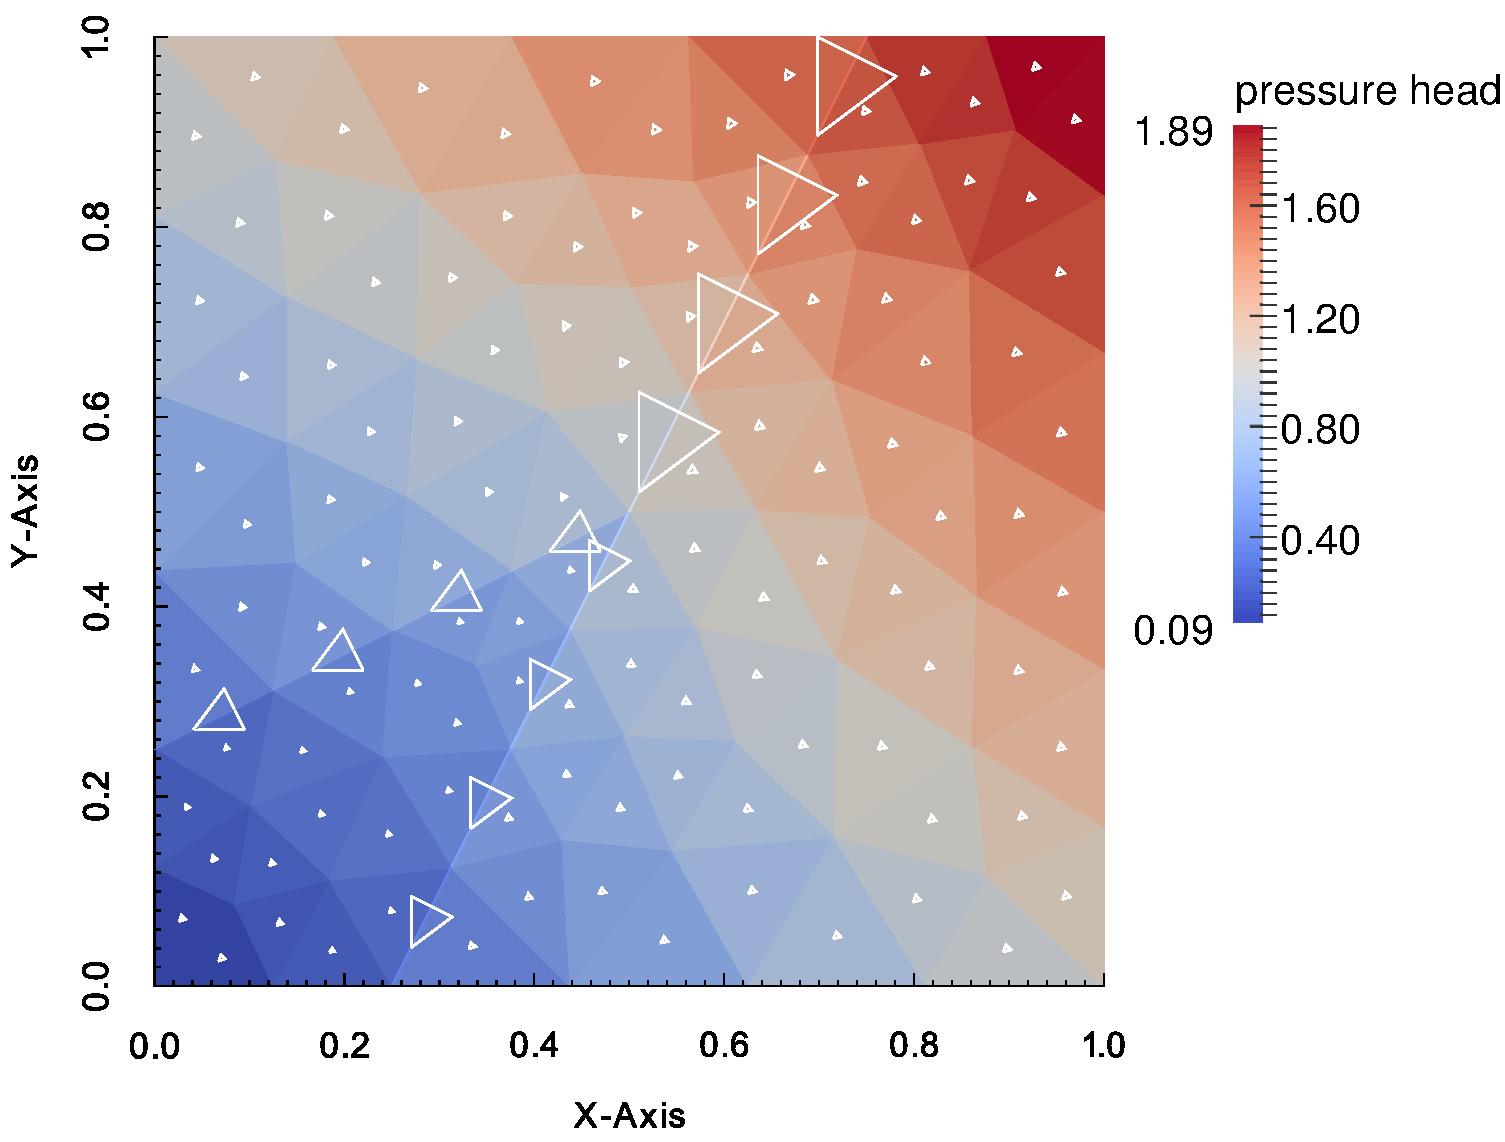
\includegraphics[width=\textwidth]{\fig/03_flow.pdf}
        % 03_flow.pdf: no raster
        \caption{Elementwise pressure head and\\velocity field denoted by triangles.\\ (Steady flow.)}
        \label{fig:tut-flow}
    \end{subfigure}
    ~
    \begin{subfigure}[b]{0.48\textwidth}
        \centering
        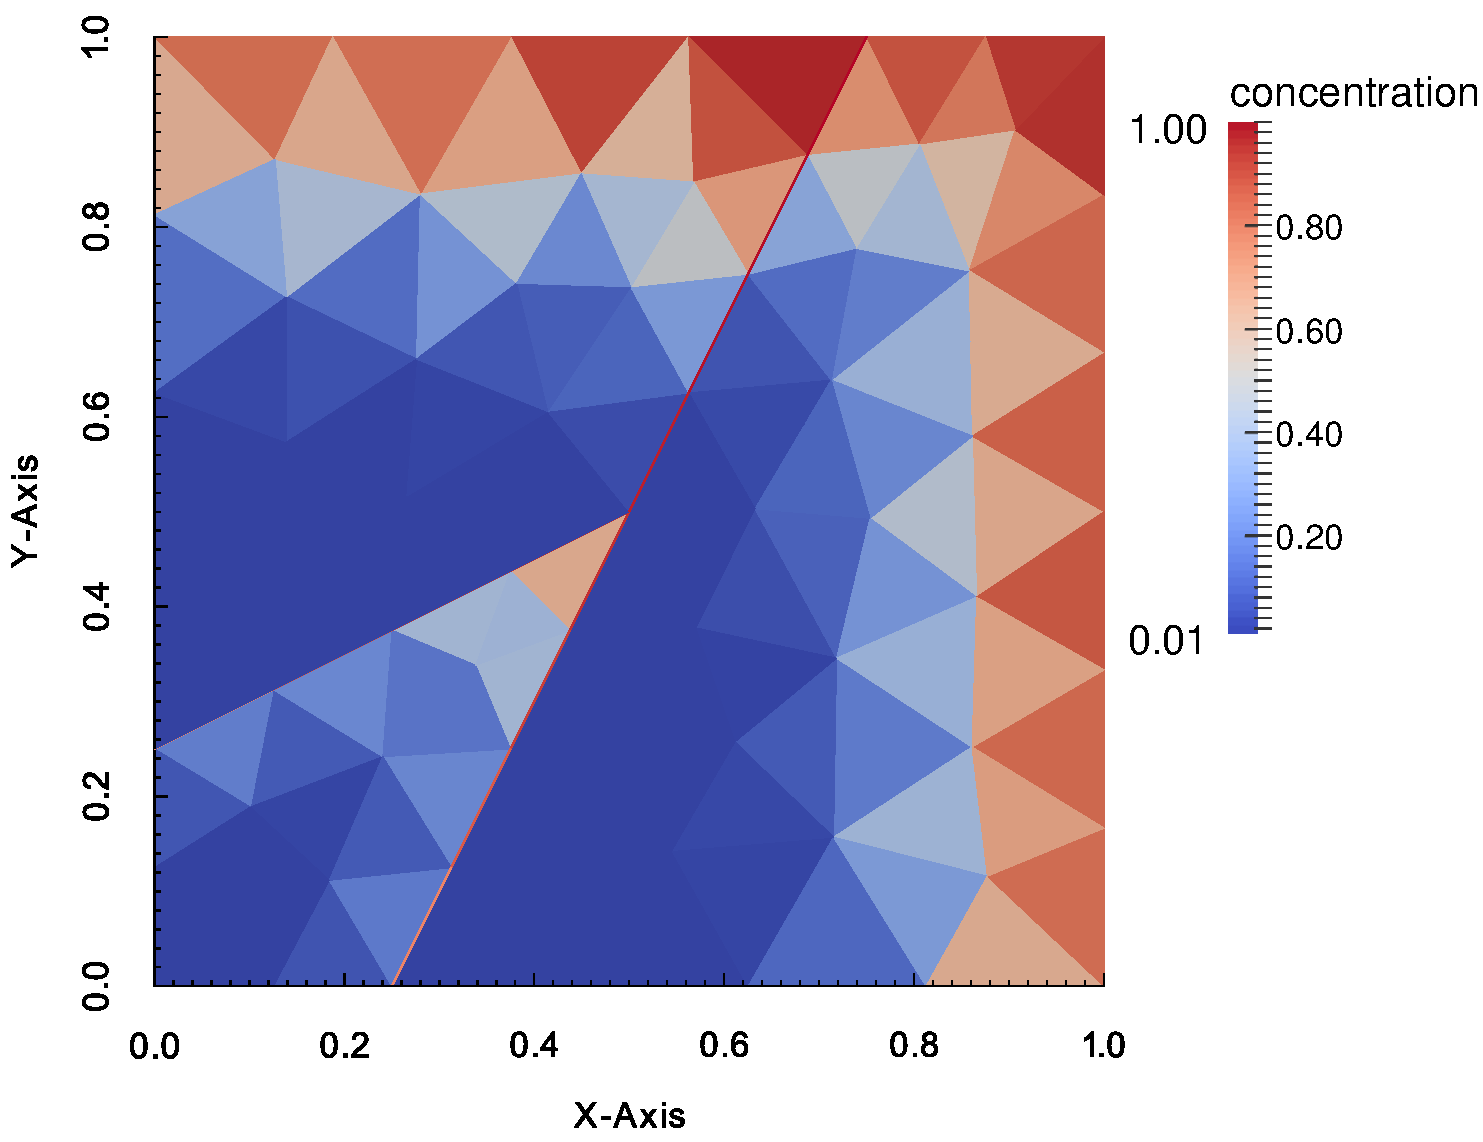
\includegraphics[width=\textwidth]{\fig/03_trans.pdf}
        % 03_trans.pdf: no raster
        \caption{Propagation of U235 from the inflow part of the boundary. \\ (At the time $9\cdot10^{5}$ s.)}
        \label{fig:tut-trans}
    \end{subfigure}
    \caption{Results of the tutorial problem.}
    \label{fig:tutorial}
\end{figure}


In the following chapter we describe mathematical models used in Flow123d.
Then in chapter \ref{chapter:file-formats} we briefly describe structure of individual input files, in particular the main CON file.
The complete description of the CON format is given in chapter \ref{chapter:input-tree-reference}.


\chapter[Mathematical Models of Physical Reality]{Mathematical Models \\of Physical Reality}
\label{chapter:mathematical_models}

Flow123d provides models for Darcy flow in porous media as well as for the transport and reactions of solutes. In this section, we describe 
mathematical formulations of these models together with physical meaning and units of all involved quantities. In the first section we present 
basic notation and assumptions about computational domains and meshes that combine different dimensions. In the next section we
derive approximation of thin fractures by lower dimensional interfaces for a general transport process. Latter sections describe details for models of particular
physical processes.

\section{Meshes of Mixed Dimension}
Common and unique feature of all models in Flow123d is the support of
domains with mixed dimension. 
Let $\Omega_{3} \subset \Real^3$ be an open set representing continuous approximation of porous and fractured medium.
Similarly, we consider a 2D manifold $\Omega_2\subset\overline\Omega_3$, representing 2D fractures and a 1D manifold $\Omega_1\subset \overline\Omega_2$ of 1D channels or preferential paths (see Fig \ref{fig:multi-dim}).
We assume that $\Omega_2$ and $\Omega_1$ are polytopic (i.e. polygonal and piecewise linear, respectively).
For every dimension $d=1,2,3$, we introduce a triangulation $\mathcal{T}_{d}$ of the open set $\Omega_d$
that consists of finite elements $T_{d}^{i},$\ $i = 1,\dots,N_{E}^{d}$.
The elements are simplices, i.e. lines, triangles and tetrahedra, respectively.

\begin{figure}[h]
\centering
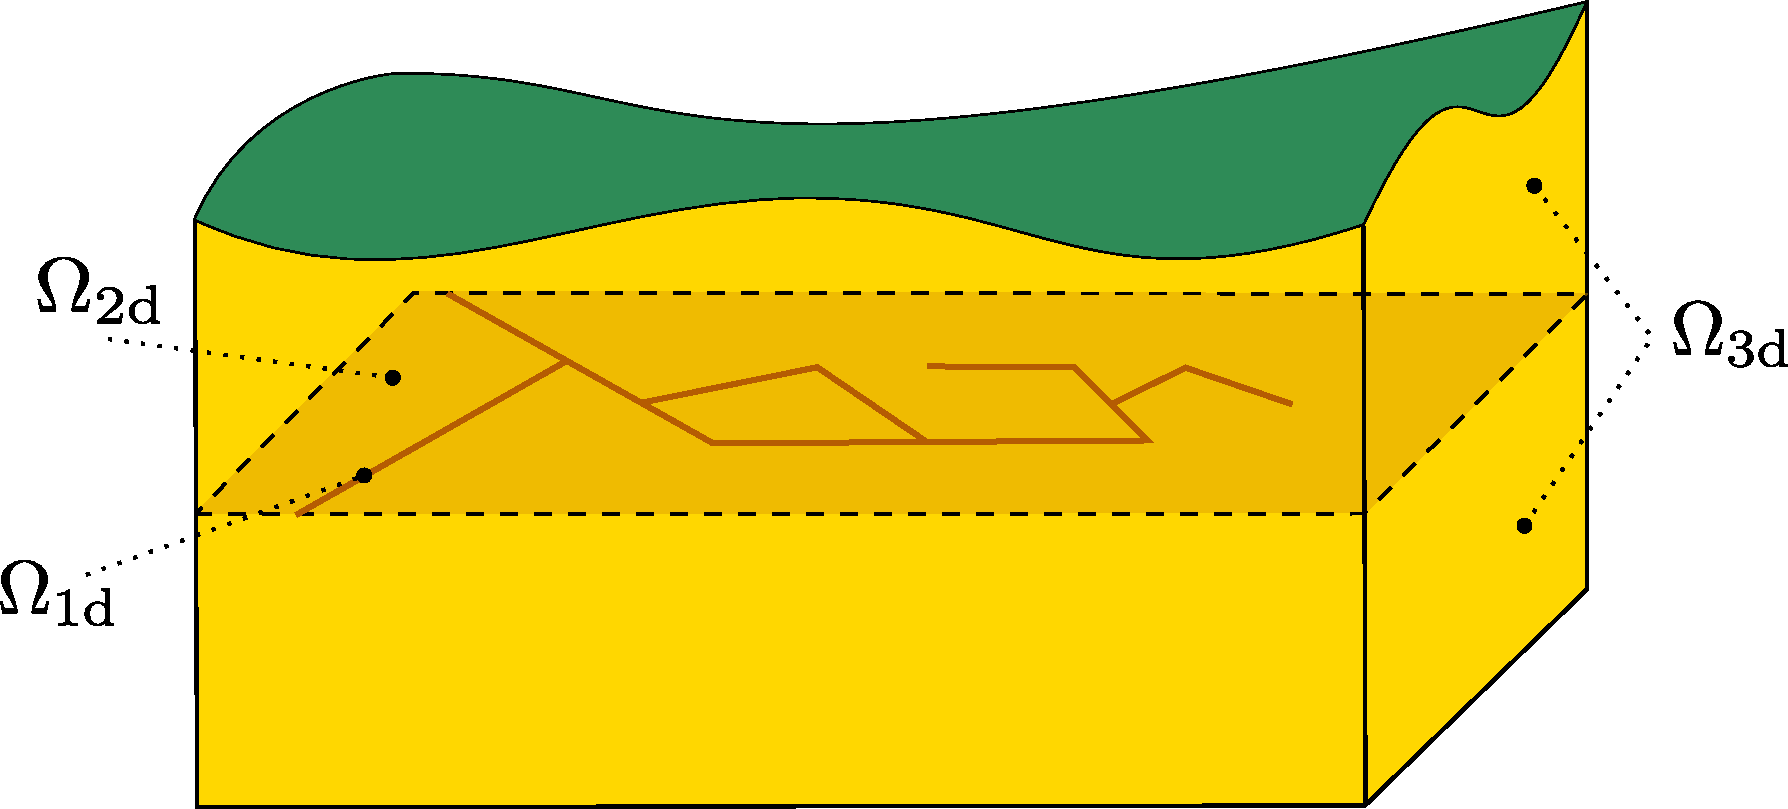
\includegraphics[width=10cm]{\fig/ground_fractures}
\caption{
    \label{fig:multi-dim}
    Scheme of a problem with domains of multiple dimensions.
}
\end{figure}

Present numerical methods require meshes satisfying the compatibility conditions
\begin{equation}
        T_{d-1}^i \cap T_d \subset \mathcal{F}_d,   \qquad \text{where } \mathcal{F}_d = \bigcup_{k} \partial T_{d}^{k}
\end{equation}
and
\begin{equation}
        T_{d-1}^i \cap \mathcal{F}_d    \text{ is either $T_{d-1}^i$ or $\emptyset$}    
\end{equation}
for every $i\in\{1,\dots, N_{E}^{d-1}\}$, $j\in\{1,\dots,N_{E}^{d}\}$,  and $d=2,3$. That is, the $(d-1)$-dimensional elements are either between $d$-dimensional elements and
match their sides or they poke out of $\Omega_d$. 

\section{Advection-Diffusion Processes on Fractures}
\label{sc:ad_on_fractures}
In this section, we shall derive a model for a general advection-diffusion process in a domain of mixed dimensions using
simple approximations inspired by the paper \citet{martin_modeling_2005}. Let us consider a fracture as a strip domain 
\[
 \Omega_f \subset [0,\delta] \times \Real^{d-1}
\]
for $d=2$ or $d=3$ and surrounding continuum domains
\[
 \Omega_1 \subset (-\infty,0)\times \Real^{d-1},
 \Omega_2 \subset (\delta,\infty)\times \Real^{d-1}.
\]
Further, we denote by $\gamma_i$, $i=1,2$ the fracture faces common with domains $\Omega_1$ and $\Omega_2$ respectively.
By $x$, $\vc y$ we denote normal and tangential coordinate of a point in $\Omega_f$. 
We consider the normal vector  $\vc n=\vc n_1=-\vc n_2=(1,0,0)^\top$.
An advection-diffusion process is given by equations:
\begin{align}
  \label{eq:fr:continuity}
  \prtl_t w_i + \div \vc j_i &= f_i&&  \text{on } \Omega_i,\ i=1,2,f,\\
  \label{eq:fr:flux}
  \vc j_i &= - \tn A_i\grad u_i + \vc b_i w_i&& \text{on } \Omega_i,\ i=1,2,f,\\
  \label{eq:fr:Dirichlet}
  u_i &= u_f&& \text{on } \gamma_i,\ i=1,2,\\
  \label{eq:fr:Neumann}
  \vc j_i \cdot \vc n &= \vc j_f \cdot \vc n&& \text{on } \gamma_i,\ i=1,2,
\end{align}
where $w_i=w_i(u_i)$ is the conservative quantity and $u_i$ is the principal unknown, $\vc j_i$ is the flux of $w_i$, $f_i$ is the source term,
$\tn A_i$ is the diffusivity tensor and $\vc b_i$ is the velocity field. We assume that the tensor $\tn A_f$ is symmetric positive definite 
with one eigenvector in the direction $\vc n$. Consequently the tensor has the form:
\[
 A_f = \begin{pmatrix} 
            a_n & 0  \\
            0 & \tn A_t
       \end{pmatrix}
\]
Furthermore, we assume that $\tn A_f(x, \vc y)=\tn A_f(\vc y)$ is constant in the normal direction.

Our next aim is to integrate equations on the fracture $\Omega_f$ in the normal direction 
and obtain their approximations on the surface $\gamma=\Omega_f \cap \{x=\delta/2\}$ running through the middle of the fracture. 
For the sake of clarity, we will not write subscript $f$ for quantities on the fracture. 
To make the following procedure mathematicaly correct we have to assume that functions
$\prtl_x w$, $\prtl_x \grad_{\vc y} u$, $\prtl_x \vc b_{\vc y}$ are continuous and bounded on $\Omega_f$. Here and later on 
$\vc b_x=(\vc b \cdot \vc n)\, \vc n$ is the normal part of the velocity field and $\vc b_{\vc y} = \vc b - \vc b_x$ is the tangential part.
The same notation will be used for normal and tangential part of the field $\vc q$.

We integrate \eqref{eq:fr:continuity} over the fracture opening $[0,\delta]$ and use approximations to get
\begin{equation}
    \label{eq:fracture_continuity}
   \prtl_t (\delta W) - \vc j_2 \cdot \vc n_2 - \vc j_1 \cdot \vc n_1 + \div \vc J = \delta F,
\end{equation}
where for the first term, we have used mean value theorem, first order Taylor expansion, 
and boundedness of $\prtl_x w$ to obtain approximation:
\[
    \int_0^\delta w(x,\vc y) \d x=\delta w(\xi_{\vc y}, \vc y) = \delta W(\vc y) + O(\delta^2\abs{\prtl_x w}),
\]
where
\[
    W(\vc y)=w(\delta / 2,\vc y)=w(u(\delta/2,\vc y))=w(U(\vc y)).
\]
Next two terms in \eqref{eq:fracture_continuity} come from the exact integration 
of the divergence of the normal flux $\vc j_x$.
Integration of the divergence of the tangential flux $\vc j_{\vc y}$ gives the fourth term, where we introduced
\[
\vc J(\vc y) = \int_0^\delta \vc j_{\vc y}(x, \vc y) \d x.
\]
In fact, this flux on $\gamma$ is scalar for the case $d=2$. Finally, we integrate the right-hand side to get 
\[
    \int_0^\delta f(x,\vc y) \d x = \delta F(\vc y) + O(\delta^2\abs{\prtl_x f}),\quad F(\vc y)=f(\delta/2,\vc y). 
\]


Due to the particular form of the tensor $\tn A_f$, we can separately integrate tangential and normal
part of the flux given by \eqref{eq:fr:flux}. Integrating the tangential part and using approximations
\[
    \int_0^\delta  \grad_{\vc y} u(x, \vc y) \d x = \delta \grad_{\vc y} u (\xi_{\vc y}, \vc y) 
    = \delta \grad_{\vc y} U( \vc y) + O\big( \delta^2 \abs{\prtl_x\grad_{\vc y} u} \big) 
\]
and
\[
 \int_0^\delta \big(\vc b_{\vc y} w\big)(x, \vc y) \d x 
  = \delta \vc B(\vc y) W(\vc y) + O\big(\delta^2 \abs{\prtl_x(\vc b_{\vc y} w)} \big)
\]
where
\[
  \vc B(\vc y) = \vc b_{\vc y}(\delta/2, \vc y),
\]
we obtain
\begin{equation}
    \label{eq:fracture_darcy}
   \vc J = -\tn A_t \delta \grad_{\vc y} U + \delta \vc B W + O\big(\delta^2(\abs{\prtl_x\grad_{\vc y} u}+\abs{\prtl_x(\vc b_{\vc y} w)})\big).
\end{equation}


So far, we have derived equations for the state quantities $U$ and $\vc J$ on the fracture manifold $\gamma$. In order to
get a well possed problem, we have to prescribe two conditions for boundaries $\gamma_i$, $i=1,2$. To this end, we
perform integration of the normal flux $\vc j_x$, given by \eqref{eq:fr:flux}, separately for the left and right half of the fracture.
Similarly as before we use approximations
\[
 \int_0^{\delta/2} \vc j_x \d x = (\vc j_1 \cdot \vc n_1)\frac{\delta}{2} + O(\delta^2 \abs{\prtl_x \vc j_x})
\]
and 
\[
 \int_0^{\delta/2} \vc b_x w \d x = (\vc b_1 \cdot \vc n_1)\tilde{w}_1\frac{\delta}{2} + O(\delta^2 \abs{\prtl_x \vc b_x}\abs{w} + \delta^2\abs{\vc b_x}\abs{\prtl_x w})
\]
and their counter parts on the interval $(\delta/2, \delta)$ to get
\begin{align}
    \label{eq:fracture_normal_1}
     \vc j_1 \cdot \vc n_1 &= -\frac{2a_n}{\delta} (U - u_1) + \vc b_1\cdot \vc n_1 \tilde{w}_1\\
    \label{eq:fracture_normal_2}
    \vc j_2 \cdot \vc n_2 &= -\frac{2a_n}{\delta} (U - u_2) + \vc b_2\cdot \vc n_2 \tilde{w}_2
\end{align}
where $\tilde w_i$ can be any convex combination of $w_i$ and $W$. Equations \eqref{eq:fracture_normal_1}  
and \eqref{eq:fracture_normal_2} have meaning of a semi-discretized flux from domains $\Omega_i$ into fracture.
In order to get a stable numerical scheme, we introduce a kind of upwind already on this level using a different convex 
combination for each flow direction:
\begin{align}
   \notag 
   \vc j_i \cdot \vc n_i
       = &-\sigma_i (U - u_i)      \\ 
   \notag
      &+ \big[\vc b_i\cdot \vc n_i\big]^{+} \big(\xi w_i + (1-\xi) W\big)       \\
      \label{eq:fracture_normal}
      &+ \big[\vc b_i\cdot \vc n_i\big]^{-} \big((1-\xi) w_i + \xi W\big), \qquad i=1,2
\end{align}
where $\sigma_i = \frac{2a_n}{\delta}$ is the transition coefficient and the parameter $\xi\in [\frac12, 1]$ can be used to interpolate
between upwind ($\xi = 1$) and central difference ($\xi=\frac12$) scheme. Equations \eqref{eq:fracture_continuity}, \eqref{eq:fracture_darcy}, and
\eqref{eq:fracture_normal} describe the general form of the advection-diffusion process on the fracture and its communication with 
the surrounding continuum which we shall later apply to individual processes.




\section{Darcy Flow Model} \label{sec:darcy_flow}
We consider the simplest model for the velocity of the steady or unsteady flow in porous and fractured medium given by 
the Darcy flow:
\begin{equation}
    \label{eq:darcy}
    \vc w = -\tn K \grad H \quad\text{in }\Omega_d,\ \text{for $d=1,2,3$}.
\end{equation}
Here and later on, we drop the dimension index $d$ of the quantities if it can be deduced from the context.
In \eqref{eq:darcy}, $\vc w$ \units{}{1}{-1} is \href{http://en.wikipedia.org/wiki/Superficial_velocity}{the superficial velocity},
$\tn K_d$ is the conductivity tensor, and $H$ \units{}{1}{} is the piezometric head. The velocity $\vc w_d$ is related to the flux $\vc q_d$ 
\units{}{4-d}{-1} through
\[
    \vc q_d = \delta_d \vc w_d,
\]
where $\delta_d$ \units{}{3-d}{} is the \hyperA{Flow-Darcy-MH-Data::cross-section}{cross section} coefficient,
in particular $\delta_3=1$, $\delta_2$ \units{}{1}{} is the thickness of a~fracture, and $\delta_1$ \units{}{2}{} is the cross-section of a~channel.
The flux $\vc q_d\cdot\vc n$ is the volume of the liquid (water) that passes through a~unit square ($d=3$),
unit line ($d=2$), or through a~point ($d=1$) per one second. 
The conductivity tensor is given by the product \penalty-500
$\tn K_d = k_d \tn A_d$, where $k_d>0$ \units{}{1}{-1}
 is the \hyperA{Flow-Darcy-MH-Data::conductivity}{hydraulic conductivity}  and 
$\tn A_d$  is the 
$3\times 3$ dimensionless \hyperA{Flow-Darcy-MH-Data::anisotropy}{anisotropy tensor} which has to be symmetric and positive definite.
The piezometric-head $H_d$ is related to the pressure head
$h_d$ through
\begin{equation}
    \label{eq:piezo_head}
    H_d = h_d + z
\end{equation}
assuming that the gravity force acts in the negative direction of the $z$-axis. 
Combining these relations, we get the Darcy law in the form:
\begin{equation}
    \label{eq:darcy_flux}
    \vc q = -\delta k\tn A \grad (h+z)  \qquad\text{in }\Omega_d,\ \text{for $d=1,2,3$}.
\end{equation}

Next, we employ the continuity equation for saturated porous medium and the dimensional reduction from the preceding section
(with $w=u:=H$, $\vc j:=\vc w$, $\tn A:=\tn K$ and $\vc b:=\vc 0$), which yields:
\begin{equation}
    \label{eq:continuity}
    \prtl_t (\delta S\, h) + \div \vc q = F + F_M\qquad \text{in }\Omega_d,\ \text{for $d=1,2,3$},
\end{equation}
where  $S_d$ \units{}{-1}{} is the \hyperA{Flow-Darcy-MH-Data::storativity}{storativity} and $F_d$ \units{}{3-d}{-1} is 
the source term. The extra source term $F_M$ \units{}{3-d}{-1} due to mechanics is described in \eqref{eq:fluid_source_div_u}. In our setting the principal unknowns of the system 
(\ref{eq:darcy_flux}, \ref{eq:continuity}) are the pressure head $h_d$ and the flux $\vc q_d$.


The storativity (or the volumetric specific storage) $S_d>0$ can be expressed as
\begin{equation}
  S_d = \gamma_w(\beta_r + \vartheta \beta_w),
\end{equation}
where $\gamma_w$ \units{1}{-2}{-2} is the specific weight of water, $\vartheta$ \units{}{}{} is the porosity,
$\beta_r$ is compressibility of the bulk material of the pores (rock)
and $\beta_w$ is compressibility of the water, both with units \units{-1}{1}{-2}. For steady problems, we set $S_d=0$ for all dimensions $d=1,2,3$.
The source term $F_d$ on the right hand side of \eqref{eq:continuity} consists of the volume density of the 
\hyperA{Flow-Darcy-MH-Data::water-source-density}{water source} 
 $f_d$\units{}{}{-1} and flux from the from the higher dimension. 
Precise form of $F_d$ slightly differs for every dimension and will be discussed presently.

In $\Omega_3$ we simply have $F_3  = f_3$ \units{}{}{-1}.

\subsection{Coupling on mixed meshes}
In the set $\Omega_2 \cap \Omega_3$ the fracture is surrounded by at most one 3D surface from every side.
On $\prtl\Omega_3 \cap \Omega_2$ we prescribe a~boundary condition of the Robin type:
\begin{align*}
        \vc{q}_3\cdot \vc n^{+} &= q_{32}^{+} =\sigma_{3} (h_3^{+}-h_2),\\
        \vc{q}_3\cdot \vc n^{-} &= q_{32}^{-} =\sigma_{3} (h_3^{-}-h_2),
\end{align*}
where $\vc{q}_3\cdot\vc n^{+/-}$ \units{}{1}{-1} is the outflow from $\Omega_3$, $h_3^{+/-}$ is
a trace of the pressure head in $\Omega_3$, $h_2$ is the pressure head in $\Omega_2$, and 
$\sigma_{3}$ \units{}{}{-1} is the transition coefficient given by (see section \ref{sc:ad_on_fractures} and \cite{martin_modeling_2005})
\[
\label{e:sigma3_law}
  \sigma_3 = \sigma_{32} \frac{2\tn K_2 :\vc n_2\otimes\vc n_2 }{\delta_2}.
\]
Here $\vc n_2$ is the unit normal to the fracture (sign does not matter).
On the other hand, the sum of the interchange fluxes $q_{32}^{+/-}$ forms
a volume source in $\Omega_2$.  Therefore $F_2$ \units{}{1}{-1} on the right hand side of \eqref{eq:continuity} is
given by
\begin{equation}
   \label{source_2D}
   F_2 = \delta_2 f_2 + (q_{32}^{+} + q_{32}^{-}).
\end{equation}

The communication between $\Omega_2$  and  $\Omega_1$ is similar.  However, in the 3D ambient space,
a 1D channel can join multiple 2D fractures $1,\dots, n$. Therefore, we have $n$
independent outflows from $\Omega_2$:
\begin{equation*}
        \vc{q}_2\cdot \vc n^{i} = q_{21}^{i} =\sigma_{2} (h_2^{i}-h_1),
\end{equation*}
where $\sigma_2$ \units{}{1}{-1} is the transition coefficient integrated over the width of the fracture $i$:
\[
\label{e:sigma2_law}
  \sigma_2 = \sigma_{21} \frac{2\delta_2^2\tn K_1:{\vc n_1^i}\otimes{\vc n_1^i}}{\delta_1}.
\]
Here $\vc n_1^i$ is the unit normal to the channel that is tangential to the fracture $i$.
Sum of the fluxes forms a~part of $F_1$ \units{}{2}{-1}:
\begin{equation}
   \label{source_1D}
   F_1 = \delta_1 f_1 + \sum_{i=1}^n q_{21}^{i}. 
\end{equation}
We remark that the direct communication between 3D and 1D (e.g. model of a~well) is not supported yet.
The \hyperA{Flow-Darcy-MH-Data::sigma}{transition coefficients} 
{$\sigma_{32}$} \units{}{}{} and
{$\sigma_{21}$} \units{}{}{} are independent scaling parameters which represent 
the ratio of the crosswind and the tangential conductivity in the fracture. For example, in the case of impermeable film
on the fracture walls one may choice $\sigma_{32} < 1$.

\subsection{Boundary conditions}
In order to obtain unique solution we have to prescribe boundary conditions.
Currently we consider a~disjoint decomposition of the boundary
\[
    \prtl\Omega_d = \Gamma_d^D \cup \Gamma_d^{TF} \cup \Gamma_d^{Sp} \cup \Gamma_d^{Ri}
\]
where we support the following
\hyperA{Flow-Darcy-MH-Data::bc-type}{types of boundary conditions}:

{\bf Dirichlet} boundary condition
\[
    h_d = h_d^D        \text{ on }\Gamma_d^D,
\]
where $h_d^D$ \units{}{1}{} is the \hyperA{Flow-Darcy-MH-Data::bc-pressure}{boundary pressure head} .
Alternatively one can prescribe the \hyperA{Flow-Darcy-MH-Data::bc-piezo-head}{boundary piezometric head}
$H_d^D$ \units{}{1}{} related to the pressure head through \eqref{eq:piezo_head}.

{\bf Total flux} boundary condition (combination of Neumann and Robin type)
\[
    -\vc q_d \cdot \vc n = \delta_d\left(q_d^N + \sigma_d^R ( h_d^R - h_d)\right)        \text{ on }\Gamma_d^{TF},
\]
where $q_d^N$ \units{}{1}{-1} is the \hyperA{Flow-Darcy-MH-Data::bc-flux}{surface density of the water inflow},
$h_d^R$ \units{}{1}{} is the \Alink{Flow-Darcy-MH-Data::bc-pressure}{boundary pressure head} and
$\sigma_d^R$ \units{}{}{-1}  
is the \hyperA{Flow-Darcy-MH-Data::bc-robin-sigma}{transition coefficient}.
As before one can also prescribe the \Alink{Flow-Darcy-MH-Data::bc-piezo-head}{boundary piezo head}
$H_d^R$ to specify $h_d^R$.

{\bf Seepage face} condition is used to model a~surface with possible springs:
\begin{equation}\label{eq:seepage}
    h_d \le h_d^S\quad \text{and} \quad -\vc q_d \cdot \vc n \le \delta_d q_d^N
\end{equation}
while the equality holds in at least one inequality. The \hyperA{Flow-Darcy-MH-Data::bc-switch-pressure}{switch pressure head} 
$h_d^S$ \units{}{1}{} can alternatively be given by \hyperA{Flow-Darcy-MH-Data::bc-switch-piezo-head}{switch piezometric head}.

The first inequality in \eqref{eq:seepage}
with the default value $h_d^S=0$ disallows non-zero water height on the surface, the later
inequality with default value $q_d^N=0$ allows only outflow from the domain (i.e. spring).
In practice one may want to allow given water height $h_d^S$ or given infiltration (e.g. precipitation-evaporation) $q_d^N$.

{\bf River} boundary condition models free water surface with bedrock of given conductivity. 
We prescribe:
\begin{align}
  -\vc q_d \cdot \vc n &= \delta_d\left(\sigma_d^R ( H_d - H_d^D) + q_d^N\right), \quad \text{for } H_d \ge H_d^S,\\
  -\vc q_d \cdot \vc n &= \delta_d\left(\sigma_d^R ( H_d^S - H_d^D)+q_d^N\right), \quad \text{for } H_d < H_d^S,
\end{align}
where $H_d$ is piezometric head.
The parameters of the condition are given by similar fields of other boundary conditions: 
the \hyperA{Flow-Darcy-MH-Data::bc-robin-sigma}{transition coefficient} of the bedrock $\sigma_d^R$ \units{}{}{-1}, 
the piezometric head of the water surface given as \Alink{Flow-Darcy-MH-Data::bc-piezo-head}{boundary piezometric head}  $H_d^D$ \units{}{1}{},
the head of the bottom of the river given as the \Alink{Flow-Darcy-MH-Data::bc-switch-piezo-head}{switch piezometric head} 
$H_d^S$ \units{}{1}{}. The boundary flux $q_d^N$ is zero by default, but can be used to express approximation of the seepage face condition 
(see discussion below).  The piezometric heads  $H_d^S$ and $H_d^R$ may be alternatively 
given by pressure heads $h_d^S$ and $h_d^R$, respectively.

The physical interpretation of the condition is as follows. For the water level $H_d$ above the bottom of the river $H_d^S$ the infiltration is given 
as Robin boundary condition with respect to the surface of the river $H_d^D$. 
For the water level below the bottom the infiltration is given by the water column of the river and transition coefficient of the bedrock.

The river could be used to approximate the seepage face condition in the similar way as the Robin boundary condition with large $\sigma$ 
can approximate Dirichlet boundary condition. We rewrite the condition as follows
\begin{align}
  -\vc q_d \cdot \vc n &= \delta_d\left(\sigma_d^R ( h_d - h_d^D) + q_d^N\right), \quad \text{for } -\vc q_d \cdot \vc n \ge \delta_d\left(\sigma_d^R ( h_d^S - h_d^D) + q_d^N\right),\\
  -\vc q_d \cdot \vc n &= \delta_d\left(\sigma_d^R ( h_d^S - h_d^D)+q_d^N\right), \quad \text{for } h_d < h_d^S.
\end{align}
Now if we take $h_d^S=h_d^D$, we obtain
\begin{align}
  -\vc q_d \cdot \vc n &= \delta_d\left(\sigma_d^R ( h_d - h_d^S) + q_d^N\right), \quad \text{for } -\vc q_d \cdot \vc n \ge \delta_d q_d^N,\\
  -\vc q_d \cdot \vc n &= \delta_d q_d^N, \quad \text{for } h_d < h_d^S,
\end{align}
where the first equation approximates $h_d = h_d^S$ if $\sigma_d^R$ is sufficiently large.

% \tbd{TODO: Once we implement mixing of BC on  a~single element. This may be usefull. Mixing seepage and river condition on single element using weighting.
% \begin{align}
%   \vc q_d \cdot \vc n &= \alpha \sigma_d^R ( H_d - H_d^D) + (1-\alpha) \sigma_{big}(H_d - H_d^S), \quad \text{for} H_d \ge H_d^S,\\
%   \vc q_d \cdot \vc n &= \alpha \sigma_d^R ( H_d^S - H_d^D)+(1-\alpha) q_d^N, \quad \text{for} H_d < H_d^S,
% \end{align}
% Since $\alpha$ is small and $\sigma_{big} \gg \sigma_d^R$ the first equation can be simplified to 
% \[
%     \vc q_d \cdot \vc n = \sigma_{big}(H_d - H_d^S) + \alpha \sigma_d^R ( H_d^S - H_d^D)+(1-\alpha) q_d^N, \quad \text{for} H_d \ge H_d^S,
% \]
% where the additional terms are to preserve continuity of the condition in the switch point.
% }

%This boundary condition models small scale free water surface, namely a~watercourse.
%To begin with consider a~small scale case where elements have scale of the width of the watercourse and the boundary match the free water surface of the water course.
%In such a~case we can prescribe the boundary condition:
%\[
%  h_d \le h_r\quad \text{and}\quad \vc q_d \cdot \vc n \ge \sigma (h - h_r)
%\]
%where $\sigma$ is a~transmissivity of the river bedrock and $h_r=0$ is the height of the water column above the discrete boundary.
%This condition use the information about water depth $h_0$ clearly can not be smaller then the pressure head at the same place. However, if the pressure head is 
%smaller, we do not allow arbitrary infiltration as in the seepage face boundary condition, but limit the infiltration by the transmissivity of the bedrock. 
%Next, if discrete boundary do not match the free surface of height $H_r$, we should rather use the piezometric head in boundary condition, getting:
%\begin{equation}
%  \label{BC:river_raw}
%  H_d \le H_r\quad \text{and}\quad \vc q_d \cdot \vc n \ge \sigma (H - H_r).
%\end{equation}
%Finally, let us assume elements significantly larger then width of the watercourse. Let, $A_e$ be the surface of a~boundary element face
%containing a~water source with the surface $A_R=\alpha_r A_e$. We want to combine the seepage face condition out of the watercourse with 
%the river condition \eqref{BC:river_raw} in to single condition. The inequality for the flux is weighted by the area:
%\[
%   \vc q\cdot \vc n \ge \alpha_r \sigma(H-H_r) + (1-\alpha_r)q_i
%\]
%where $q_i$ is the infiltration (negative) or evaporation (positive) on the surface out of the watercourse. Similarly, we consider
%\[
%  H_d \le H_c = (\alpha_r) H_r + (1-\alpha_r) H_s
%\]
%where the critical piezometric head $H_c$ is a~weighted average of the river head and the average height $H_s$ of the real surface.
%
%
%Parameters: $\alpha_r$ \units{}{}{} the \hyperA{Flow-Darcy-MH-Data::bc-river-fraction}{river surface fraction}, $H_r$ \units{1}{}{} 
%the \hyperA{Flow-Darcy-MH-Data::bc-river-head}{river head}, 
%alternatively $H_c=H_d^D$ \units{1}{}{} the critical piezometric head or $h_c=h_d^D$ \units{1}{}{} the critical pressure head, $q_i=q_d^N$ \units{}{4-d}{-1}
%the infiltration or evapotranspiration rate, $\sigma=\sigma_d^R$ \units{}{3-d}{-1}  
%the \hyperA{Flow-Darcy-MH-Data::bc-robin-sigma}{transition coefficient} of the bedrock.
%
%Implementation: prescribing $\alpha_r$ as a~field makes only sense for the case of element-wise field since the value depends on the cross-section 
%of the river and the boundary element. Ultimate goal should be to prescribe river as an 1D line and set width of the river on its elements. Then we can 
%modify non-compatible intersection algorithms to compute value of $\alpha_r$ for individual elements.
%


\subsection{Steady and unsteady Darcian flow}

By default, the \hyperA{Flow-Darcy-MH-Data::storativity}{storativity} is zero which means that the flow is calculated steady.
If, in addition, some input fields are time-dependent, a~sequence of steady problems is calculated for times in which the data change.
When storativity is nonzero, the problem becomes unsteady and one has to specify the initial condition and the computational time interval.

\subsection{Initial condition}
For unsteady problems one has to specify an initial condition in terms of the 
\hyperA{Flow-Darcy-MH-Data::init-pressure}{initial pressure head}
$h_d^0$ \units{}{1}{}
or the \hyperA{Flow-Darcy-MH-Data::init-piezo-head}{initial piezometric head}
$H_d^0$ \units{}{1}{}.

\subsection{Water balance}
The equation \eqref{eq:continuity} satisfies the volume balance of the liquid in the following form:
\[ V(0) + \int_0^t s(\tau) \,d\tau + \int_0^t f(\tau) \,d\tau = V(t) \]
for any instant $t$ in the computational time interval.
Here
$$ V(t) := \sum_{d=1}^3\int_{\Omega^d}(\delta S h)(t,\vc x)\,d\vc x, $$
$$ s(t) := \sum_{d=1}^3\int_{\Omega^d}F(t,\vc x)\,d\vc x, $$
$$ f(t) := -\sum_{d=1}^3\int_{\partial\Omega^d}\vc q(t,\vc x)\cdot\vc n(\vc x) \,d\vc x $$
is the volume \units{}{3}{}, the volume source \units{}{3}{-1} and the volume flux \units{}{3}{-1} of the liquid at time $t$, respectively.
The volume, flux and source on every geometrical region is calculated at each output time and the values together with the control sums are written to the \Alink{Balance::file}{file} \texttt{water\_balance.\{dat\textbar txt\}}.
If, in addition, \Alink{Balance::cumulative}{cumulative} is set to true then the time-integrated flux and source is written.
The format of balance output is described in Section \ref{sec:balance_output}.

\subsection{Richards Equation}
This section contains a~preliminary documentation to the unsaturated water flow model. We use the Richards equation in the form:

\begin{equation}
 \prtl_t \delta \theta_t + \div \vc q = F\quad \in\Omega_d, \text{ for } d=1,2,3
\end{equation}
where the total water content $\theta_t(h)$ \units{}{}{} is a~function of the principal unknown $h$ and the water flux $\vc q$ is given by \eqref{eq:darcy_flux} 
in which the conductivity $k_d$ is function of the pressure head $h$ as well.
Currently the total water content is given as:
\begin{equation}
    \theta_t(h) = \theta(h) + Sh
\end{equation}
where $S$ is the storativity and $\theta(h)$ is the water content. The functions $\theta(h)$ and $k(h)$ are given by the chosen soil model.
Two soil models are currently supported.

\subsubsection{van Genuchten}
Classical van Genuchten model use:
\[
    \theta(h) = (\theta_s-\theta_r)\theta_e + \theta_r,\quad \theta_e = (1+ (\alpha h)^n)^m
\]
for the negative pressure head $h<0$ and $\theta = \theta_s$ for $h\ge 0$.

The model parameters are:
    $\theta_s$ \units{}{}{} the saturated water content,
    $\theta_r$ \units{}{}{} the residual water content,
    $\alpha$ \units{}{-1}{} the pressure scaling parameter,
    $n$ \units{}{}{} the exponent parameter.
The exponent $m$ is taken as $1/n-1$ and $\theta_e$ \units{}{}{} is called the effective water content.

The conductivity function $k(h)$ is then derived from the capillary model due to Mualem with result:
\[
    k(h) = \theta_e^{0.5} \left[ \frac{1-F(\theta)}{1-F(\theta_s)} \right]^2,\quad F(\theta)= \left[ 1- \theta_e^{1/m} \right]^m
\]
In fact we use slight modification due to Vogel and Císlerová where the saturation happens at some pressure head slightly smaller then zero.
Then the water content curve is given by 
\[
    \theta(h) = (\theta_m-\theta_r)\theta_e + \theta_r,
\]
for $h< h_s$ and $\theta = \theta_s$ for $h\ge h_s$. Currently the fraction $\theta_m / \theta_s$ is fixed to $0.001$.

\subsubsection{Irmay}
The model used for bentonite is due to Irmay and use simple power relation for the conductivity:
\[
   k(h) = \theta_e^{3}.
\]


\subsection{Coupling of dimensions for non-conforming meshes}
Version 3.0.0 introduce an experimental support for the non-conforming meshes of mixed dimension. 
In particular 1D-2D coupling is supported in the 2D ambient space and 2D-3D and 2D-2D coupling is 
supported for the 3D ambient space. Non-conforming coupling is supported only by the Darcy flow model
and lower dimensional elements can not represent barriers, i.e. we consider that the pressure 
and the velocity fields are continuous across the lower dimensional fractures. Search for the non-conforming intersections 
and assembly of the associated terms in the weak formulation is turned on by the key \hyperA{Flow-Darcy-MH::mortar-method}{mortar\_method}.
One of two methods can be selected: $P0$ method is faster but can be a~bit unstable for coarse meshes, $P1$ method should be more robust.

    



% ***************************************** SYMBOLS
\def\abs#1{\lvert#1\rvert}
\def\argdot{{\hspace{0.18em}\cdot\hspace{0.18em}}}
\def\avg#1{\left\{#1\right\}_\omega}
\def\D{{\tn D}}
\def\div{\operatorname{div}}
\def\Eh{\mathcal E_h}       % edges of \Th
\def\Ehcom{\mathcal E_{h,C}}         % edges of \Th on interface with lower dimension
\def\Ehdir{\mathcal E_{h,D}}         % Dirichlet edges of \Th
\def\Ehint{\mathcal E_{h,I}}       % interior edges of \Th
\def\grad{\nabla}
\def\jmp#1{[#1]}
\def\n{\vc n}
\def\vc#1{\mathbf{\boldsymbol{#1}}}     % vector
\def\R{\mathbb R}
\def\sc#1#2{\left(#1,#2\right)}
\def\Th{\mathcal T_h}       % triangulation
\def\th{\vartheta}
\def\tn#1{{\mathbb{#1}}}    % tensor
\def\Tr{\operatorname{Tr}}
\def\where{\,|\,}
%***************************************************************************


\section{Transport of substances}
\label{sc:transport_model}

The motion of substances dissolved in water is governed by the \emph{advection}, and the \emph{hydrodynamic dispersion}.
In $\Omega_d$, $d\in\{1,2,3\}$, we consider the following system of mass balance equations\footnote{For $d\in\{1,2\}$ this form can be derived as in Section \ref{sc:ad_on_fractures} using $w:=\delta\th c^i$, $u:=c^i$, $\tn A:=\delta\th\tn D^i$, $\vc b:=\vc v=\frac{\vc q}{\th\delta}$.}:
\begin{equation}
    \label{e:ADE}
   \partial_t ( \delta \th c^i) + \div ( \vc q c^i ) - \div (\th \delta \D^i \grad c^i ) = F_S^i + F^c_C(c^i) + F_R(c^1,\dots, c^s).
\end{equation}
The principal unknown is the concentration $c^i$ \units{1}{-3}{} of a substance $i\in\{1,\dots, s\}$, which means weight of the substance in unit volume of the water.
Other quantities are:
\begin{itemize}

\item $\th$ \units{}{}{} is the \hyperA{SoluteTransport-DG-Data::porosity}{porosity}, i.e. fraction of space occupied by water and the total volume.
\item The hydrodynamic dispersivity tensor $\D^i$ \units{}{2}{-1} has the form
\begin{equation} 
  \label{eqn:transport_disp}
  \D^i =D_m^i \tau \tn I + \abs{\vc v}\left(\alpha_T^i \tn I + (\alpha_L^i - \alpha_T^i) \frac{\vc v \otimes \vc v}{\abs{\vc v}^2}\right),
\end{equation}
which represents (isotropic) molecular diffusion, and mechanical dispersion in longitudal and transversal direction to the flow.
Here $D_m^i$ \units{}{2}{-1} is the \hyperA{SoluteTransport-DG-Data::diff-m}{molecular diffusion coefficient} of the $i$-th substance (usual magnitude in clear water is $10^{-9}$), $\tau=\th^{1/3}$ is the tortuosity (by \cite{millington_quirk}), $\alpha_L^i$ \units{}{1}{} and $\alpha_T^i$ \units{}{1}{} is the \hyperA{SoluteTransport-DG-Data::disp-l}{longitudal dispersivity} and the \hyperA{SoluteTransport-DG-Data::disp-t}{transverse dispersivity}, respectively.
Note that although we allow dispersivities to have different values for different substances, it is often assumed that they are intrinsic parameters of the porous medium.
Finally, $\vc v$ \units{}{1}{-1} is the \emph{microscopic} water velocity, related to the Darcy flux $\vc q$ by the relation $\vc q = \th\delta\vc v$.
The value of $D_m^i$ for specific substances can be found in literature (see e.g. \cite{cislerova_vogel}).
For instructions on how to determine $\alpha_L^i$, $\alpha_T^i$ we refer to \cite{marsily,domenico_schwartz}.

\item $F_S^i$ \units{1}{-d}{-1} represents the density of concentration sources.
Its form is:
\begin{equation}
 F_S^i = \delta f^i_S + \delta(c_S^i-c^i)\sigma_S. \label{eqn:transport_sources}
\end{equation}
Here $f_S^i$ \units{1}{-3}{-1} is the \hyperA{SoluteTransport-DG-Data::sources-density}{density of concentration sources}, $c_S^i$ \units{1}{-3}{} is an \hyperA{SoluteTransport-DG-Data::sources-conc}{equilibrium concentration} and $\sigma_S^i$ \units{}{}{-1} is the \hyperA{SoluteTransport-DG-Data::sources-sigma}{concentration flux}.

\item $F^c_C(c^i)$ \units{1}{-d}{-1} is the density of concentration sources due to exchange between regions with different dimensions, see \eqref{e:FC} below.

\item The reaction term $F_R(\dots)$ \units{1}{-d}{-1} is thoroughly described in the next section \ref{sec:reaction_term}.
\end{itemize}



\paragraph{Initial and boundary conditions.}
At time $t=0$ the concentration is determined by the \hyperA{SoluteTransport-DG-Data::init-conc}{initial condition}
$$ c^i(0,\vc x) = c^i_0(\vc x). $$
The physical boundary $\partial\Omega_d$ is decomposed into the parts $\Gamma_I\cup\Gamma_D\cup\Gamma_N\cup\Gamma_R$, which may change during simulation time.
The first part $\Gamma_I$ is further divided into two segments:
\begin{align*}
\Gamma_I^+(t) &= \{\vc x\in \partial\Omega_d\where \vc q(t,\vc x)\cdot\vc n(\vc x)<0\},\\
\Gamma_I^-(t) &= \{\vc x\in \partial\Omega_d\where \vc q(t,\vc x)\cdot\vc n(\vc x)\ge 0\},
\end{align*}
where $\vc n$ stands for the unit outward normal vector to $\partial\Omega_d$.
We prescribe the following boundary conditions:
On the inflow parts $\Gamma_I^+\cup\Gamma_D$, the user must provide \hyperA{SoluteTransport-DG-Data::bc-conc}{Dirichlet boundary condition} $c_D^i$ for concentrations:
$$ c^i = c^i_D \mbox{ on }\Gamma_I^+\cup\Gamma_D. $$
On $\Gamma_I^-$ we impose homogeneous Neumann boundary condition:
$$ -\th\delta\D^i\nabla c^i\cdot\vc n = 0 \mbox{ on }\Gamma_I^-, $$
on $\Gamma_N$ we impose Neumann boundary condition with user-defined \hyperA{SoluteTransport-DG-Data::bc-flux}{concentration flux} $f^i_N$:
$$ -\th\delta\D^i\nabla c^i\cdot\vc n = f^i_N \mbox{ on }\Gamma_N, $$
and finally on $\Gamma_R$ we impose Robin boundary condition through \hyperA{SoluteTransport-DG-Data::bc-robin-sigma}{transition parameter} $\sigma^i_R$ and \hyperA{SoluteTransport-DG-Data::bc-conc}{reference concentration} $c^i_D$:
$$ -\th\delta\D^i\nabla c^i\cdot\vc n = \sigma^i_R(c^i-c^i_D) \mbox{ on }\Gamma_R. $$






\paragraph{Communication between dimensions.}
Transport of substances is considered also on interfaces of physical domains with adjacent dimensions (i.e. 3D-2D and 2D-1D, but not 3D-1D).
Denoting $c_{d+1}$, $c_d$ the concentration of a given substance in $\Omega_{d+1}$ and $\Omega_d$, respectively, the comunication on the interface between $\Omega_{d+1}$ and $\Omega_d$ is described by the quantity
\begin{equation}
  \label{e:inter_dim_flux}
  q^c_{d+1,d} = \sigma^c_{d+1,d} \frac{\delta_{d+1}^2}{\delta_d}2\th_d\D_d:\n\otimes\n ( c_{d+1} - c_d) + \begin{cases}q^l_{d+1,d} c_{d+1} & \mbox{ if }q^l_{d+1,d}\ge 0,\\q^l_{d+1,d} \frac{\th_d}{\th_{d+1}} c_d & \mbox{ if }q^l_{d+1,d}<0,\end{cases}
\end{equation}
where
\begin{itemize}
\item $q^c_{d+1,d}$ \units{1}{-d}{-1} is the density of concentration flux from $\Omega_{d+1}$ to $\Omega_d$,
\item $\sigma^c_{d+1,d}$ \units{}{}{} is a \hyperA{SoluteTransport-DG-Data::fracture-sigma}{transition parameter}.
Its value determines the mass exchange between dimensions whenever the concentrations differ.
In general, it is recommended to leave the default value $\sigma^c=1$ or to set $\sigma^c=0$ (when exchange is due to water flux only).
\item $q^l_{d+1,d}$ \units{}{3-d}{-1} is the water flux from $\Omega_{d+1}$ to $\Omega_d$, i.e. $q^l_{d+1,d} = \vc q_{d+1}\cdot\n_{d+1}$.
\end{itemize}
The communication between dimensions is incorporated as the total flux boundary condition for the problem on $\Omega_{d+1}$:
\begin{equation}
\label{e:FC}
-\th\delta\D\nabla c\cdot\vc n + q^w c = q^c
\end{equation}
and a source term in $\Omega_d$:
\begin{equation}
F^c_{C3} = 0,\quad
F^c_{C2} = q^c_{32},\quad
F^c_{C1} = q^c_{21}.
\end{equation}



\paragraph{Mass balance.}
The advection-dispersion equation satisfies the balance of mass in the following form:
$$ m^i(0) + \int_0^t s^i(\tau) \,d\tau - \int_0^t f^i(\tau) \,d\tau = m^i(t) $$
for any instant $t$ in the computational time interval and any substance $i$.
Here
$$ m^i(t) := \sum_{d=1}^3\int_{\Omega^d}(\delta\th c^i)(t,\vc x)\,d\vc x, $$
$$ s^i(t) := \sum_{d=1}^3\int_{\Omega^d}F_S^i(t,\vc x)\,d\vc x, $$
$$ f^i(t) := \sum_{d=1}^3\int_{\partial\Omega^d}\left(\vc q c^i - \th\delta\D^i\nabla c^i\right)(t,\vc x)\cdot\vc n \,d\vc x $$
is the mass \units{1}{}{}, the volume source \units{1}{}{-1} and the mass flux \units{1}{}{-1} of $i$-th substance at time $t$, respectively.
The mass, flux and source on every geometrical region is calculated at each computational time step and the values together with the control sums are written to the file \texttt{mass\_balance.txt}.


\paragraph{Two transport models.}
Within the above presented model, Flow123d presents two possible approaches to solute transport.
\begin{itemize}
\item For modelling pure advection ($\tn D=0$) one can choose {\tt TransportOperatorSplitting} method, which represents an explicit in time finite volume solver. The solution process for one time step is faster, but the maximal time step is restricted. The resulting concentration is piecewise constant on mesh elements. This solver supports reaction term (involving simple chemical reactions, dual porosity and adsorption).
\item The full model including dispersion is solved by {\tt SoluteTransport\_DG}, an implicit in time discontinuous Galerkin solver. It has no restriction of the computational time step and the space approximation is piecewise polynomial, currently up to order 3. Reaction term is currently not implemented.
\end{itemize}





% ***************************************** SYMBOLS
\def\abs#1{\lvert#1\rvert}
\def\argdot{{\hspace{0.18em}\cdot\hspace{0.18em}}}
\def\avg#1{\left\{#1\right\}_\omega}
\def\D{{\tn D}}
\def\div{\operatorname{div}}
\def\Eh{\mathcal E_h}       % edges of \Th
\def\Ehcom{\mathcal E_{h,C}}         % edges of \Th on interface with lower dimension
\def\Ehdir{\mathcal E_{h,D}}         % Dirichlet edges of \Th
\def\Ehint{\mathcal E_{h,I}}       % interior edges of \Th
\def\grad{\nabla}
\def\jmp#1{[#1]}
\def\n{\vc n}
\def\vc#1{\mathbf{\boldsymbol{#1}}}     % vector
\def\R{\mathbb R}
\def\sc#1#2{\left(#1,#2\right)}
\def\Th{\mathcal T_h}       % triangulation
\def\th{\vartheta}
\def\tn#1{{\mathbb{#1}}}    % tensor
\def\Tr{\operatorname{Tr}}
\def\where{\,|\,}
%***************************************************************************

\section{Reaction term in transport}
\label{sec:reaction_term}

The {\tt TransportOperatorSplitting} method supports the reaction term $F_R(c^1,\ldots,c^s)$ on the right hand side of the equation (\ref{e:ADE}).
It can represent several models of chemical or physical nature. 
Figure \ref{fig:reaction_term} shows all possible reactional models that we support in combination with the transport process. The Operator Splitting method enables 
us to deal with the convection part and reaction term side by side. The convected quantities do not influence each other in the convectional
process and are balanced over the elements. On the other hand the reaction term relates the convected quantities and can be computed 
separately on each element.

We move now to the description of the reaction models which can be seen again in Figure \ref{fig:reaction_term}. 
The convected quantity is considered to be the concentration of substances. 
Up to now we can have \emph{dual porosity}, \emph{adsorption} (these two are more of a physical nature) and (chemical) \emph{reaction} models in the reaction term. 

\begin{figure}
  \centering
  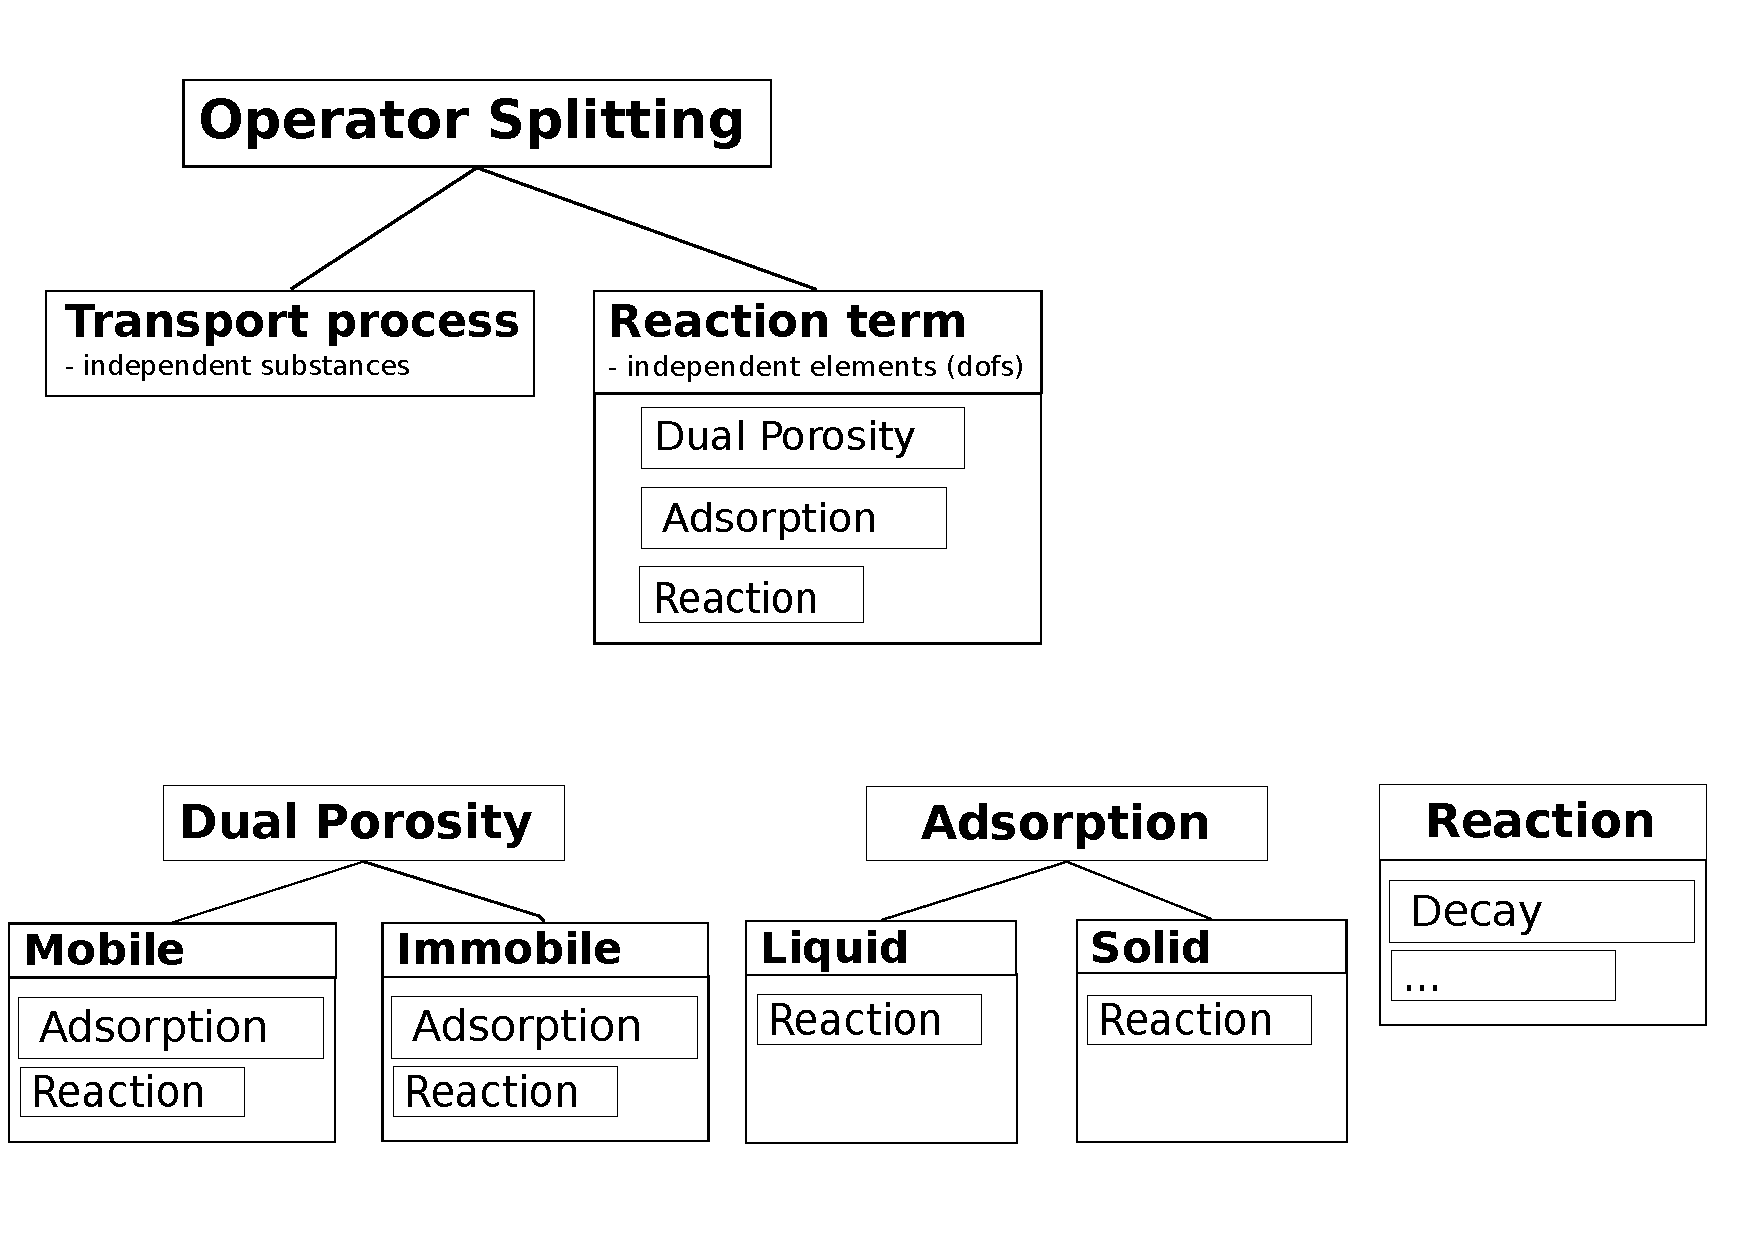
\includegraphics[width=\textwidth]{\fig/reaction_term.pdf}
  \caption{The scheme of the reaction term objects. The lines represents connections between different models. 
  The tables under model name include the possible models which can be connected to the model above.}
  \label{fig:reaction_term}
\end{figure}

The \emph{reaction} model acts only on the specified substances. It does not have its own output.

The \emph{adsorption} model describes the exchange of concentration of the substances between liquid and solid. It can be
followed by another \emph{reaction} that can run in both phases. The concentration in solid is an additional output 
of this model. See Subsection \ref{sec:sorp_math}.


The \emph{dual porosity} model, described in Subsection \ref{sec:dual_porosity}, introduces the so called immobile (or dead-end) pores in the matrix. The convection process operates only on the concentration of the substances in the mobile zone (open pores) 
and the exchange of concentrations from/to immobile zone is governed by molecular diffusion. This process can be followed by 
\emph{adsorption} model and/or chemical \emph{reaction}, both in mobile and immobile zone. The immobile concentration is an
additional output.


\subsection{Dual porosity}
\label{sec:dual_porosity}

Up to now we have described the transport equation for the single porosity model. The dual porosity model splits the mass into 
two zones -- the mobile zone and the immobile zone. Both occupy the same macroscopic volume, however on the microscopic scale, 
the immobile zone is formed by the dead-end pores, where the liquid is trapped and cannot pass through. The rest of the pore volume 
is occupied by the mobile zone. Since the liquid in the immobile pores is immobile, the exchange of the substance is only due 
to molecular diffusion. We consider simple nonequilibrium linear model:
\begin{align}
    \vartheta_m \partial_t c_m &= D_{dp} ( c_i - c_m), \label{eqn:dual_porosity_ode1}\\
    \vartheta_i \partial_t c_i &= D_{dp} ( c_m - c_i), \label{eqn:dual_porosity_ode2}
\end{align}
where $c_m$ is the concentration in the mobile zone, $c_i$ is the concentration in the immobile zone and
\hyperA{DualPorosity-Data::diffusion-rate-immobile}{$D_{dp}$} is a diffusion rate between the zones.
\hyperA{DualPorosity-Data::porosity-immobile}{$\vartheta_i$}~denotes porosity of the immobile zone  and 
$\hyperlink{TransportOperatorSplitting-Data::porosity::B}{\vartheta_m} = \vartheta$ the mobile porosity from transport equation \eqref{e:ADE}.

The analytic solution of the system of differential equations at time $t$ with initial conditions $c_m(0)$ and $c_i(0)$ is
\begin{align}
     c_m(t) &= (c_m(0) - c_a(0)) \exp\left(- D_{dp}\left(\frac{1}{\vartheta_m} + \frac{1}{\vartheta_i}\right) t \right) + c_a(0), 
     \label{eqn:dual_porosity_anal1}\\
     c_i(t) &= (c_i(0) - c_a(0)) \exp\left(- D_{dp}\left(\frac{1}{\vartheta_m} + \frac{1}{\vartheta_i}\right) t \right) + c_a(0),
     \label{eqn:dual_porosity_anal2}
\end{align}
where $c_a$ is the weighted average
\[
  c_a = \frac{\vartheta_m c_m + \vartheta_i c_i}{\vartheta_m + \vartheta_i}.
\]

If the time step is large we use the analytic solution to compute new values of concentrations. 
Otherwise we replace the time derivatives in \eqref{eqn:dual_porosity_ode1} and \eqref{eqn:dual_porosity_ode2} 
by first order forward differences and we get the classical Euler scheme
\begin{align}
  c_m(t^+) = \frac{D_{dp} \Delta t}{\vartheta_m}(c_i(t) - c_m(t)) + c_m(t), \\
  c_i(t^+) = \frac{D_{dp} \Delta t}{\vartheta_i}(c_m(t) - c_i(t)) + c_i(t), \\
\end{align}
where $\Delta t = t^+ - t$ is the time step. 

The condition on the size of the time step is derived from the Taylor exapansion of 
\eqref{eqn:dual_porosity_anal1} or \eqref{eqn:dual_porosity_anal2}, respectively. We neglect the higher order 
terms and we want the second order term smaller than given scheme tolerance 
\hyperA{DualPorosity::scheme-tolerance}{$tol$} relatively to $c_a$
\begin{equation}
  (c_m(0) - c_a(0))
  \frac{ D_{dp}^2 (\Delta t)^2 \left(\frac{\vartheta_m + \vartheta_i}{\vartheta_m \vartheta_i}\right)^2}{2}
  \frac{1}{c_a} \leq tol. \\
\end{equation}
Then we transform the above inequation into the following condition which is tested in the program
\begin{equation} \label{eqn:euler_scheme_condition}
  \max(|c_m(0) - c_a(0)|, |c_i(0) - c_a(0)|) \leq 
  2 c_a \left(\frac{\vartheta_m \vartheta_i}{D_{dp} \Delta t (\vartheta_m + \vartheta_i)}\right)^2 tol. \\
\end{equation}
If the inequation \eqref{eqn:euler_scheme_condition} is not satisfied then the analytic 
solution is used.
 

\subsection{Equilibrial adsorption}
\label{sec:sorp_math}

The simulation of monolayer, equilibrial adsorption is based on the solution of two algebraic equations, namely the mass balance (in unit volume)
\begin{equation}
\label{eq:mass_balance_sorption}
\th \varrho_l c_l + (1-\th) \varrho_s M_s c_s = c_T = const.
\end{equation}
and an empirical adsorption law
\begin{equation}
\label{eq:relation_cs_cl}
c_s = f(c_l),
\end{equation}
given in terms of the so-called isotherm $f$.
Its form is determined by the parameter \hyperA{Sorption-Data::sorption-type}{\tt sorption\_type}:
\begin{itemize}
 \item ``$none$'': $f(c_l)=0$ (the adsorption model returns zero concentration in solid);
 \item ``$linear$'': $f(c_l) = k_l c_l$;
 \item ``$freundlich$'': $f(c_l) = k_F c_l^{\alpha}$;
 \item ``$langmuir$'': $f(c_l) = k_L \frac{\alpha c_l}{1 + \alpha c_l}$.
       Langmuir isotherm has been derived from thermodynamic laws. $k_L$ denotes the maximal amount 
       of sorbing specie which can be kept in an unit volume of a bulk matrix. Coefficient $\alpha$ is 
       a fraction of adsorption and desorption rate constant $\alpha = \frac{k_a}{k_d}$.
\end{itemize}

Notation:
\begin{itemize}
 \item Concentration in solid $c_s = \frac{n}{m_s}$ [mol\,$\mathrm{kg}^{-1}$], where $m_s$, $n$ is the 
       mass of solid and the molar amount of the substance in unit volume, respectively;
 \item Concentration in liquid $c_l = \frac{m}{m_l}$ \units{}{}{}, where $m_l$ is 
       the mass of liquid in unit volume. The relation between $c_l$ and the concentration $c$ from 
       transport equation \eqref{e:ADE} is $c = c_l \varrho_l$;
 \item \hyperA{Sorption::solvent-density}{$\varrho_l$}, \hyperA{Sorption-Data::rock-density}{$\varrho_s$} is the liquid (solvent) density and the solid (rock) density, respectively;
 \item \hyperA{Sorption::molar-mass}{$M_s$} denotes the molar mass of a substance;
 \item Multiplication parameters $k_i, i\in\{ l,F,L\}$ [mol\,$\mathrm{kg}^{-1}$] are given by 
       \hyperA{Sorption-Data::isotherm-mult}{\tt isotherm\_mult};
 \item Additional parameter $[\alpha] = 1$ is given by \hyperA{Sorption-Data::isotherm-other}{\tt isotherm\_other}.
\end{itemize}

Denoting
\[ \mu_l = \varrho_l \th, \quad \mu_s = M_s \varrho_s\cdot(1-\th), \]
and using \eqref{eq:relation_cs_cl}, the mass balance \eqref{eq:mass_balance_sorption} reduces to the equation
\begin{equation}
 c_T = \mu_l c_l + \mu_s f(c_l),
 \label{eq:nonlin_sorption}
\end{equation}
which can be either solved iteratively or using interpolation.
To solve \eqref{eq:nonlin_sorption} iteratively, it is very important to define the interval where 
to look for the solution (unknown $c_l$), see Figure \ref{fig:sorpce}. The lower bound is $0$ (concentration can not reach negative values). 
The upper bound is derived using a simple mapping. Let us suppose limmited 
\hyperA{Sorption::solubility}{$solubility$} of the selected transported substance and let us denote the 
limmit $\bar{c}_l$. We keep the maximal "total mass" 
$\bar{c}_T= \mu_l\cdot \bar{c}_l + \mu_s\cdot f(\bar{c}_l)$, but we dissolve all the mass to get 
maximal $c_l^{max} > \bar{c}_l$. That means $c_s = 0$ at this moment. We can slightly enlarge the interval by setting the upper bound equal to 
$c_l^{max} + const_{small}$.

\begin{figure}[ht!]
 \centering
 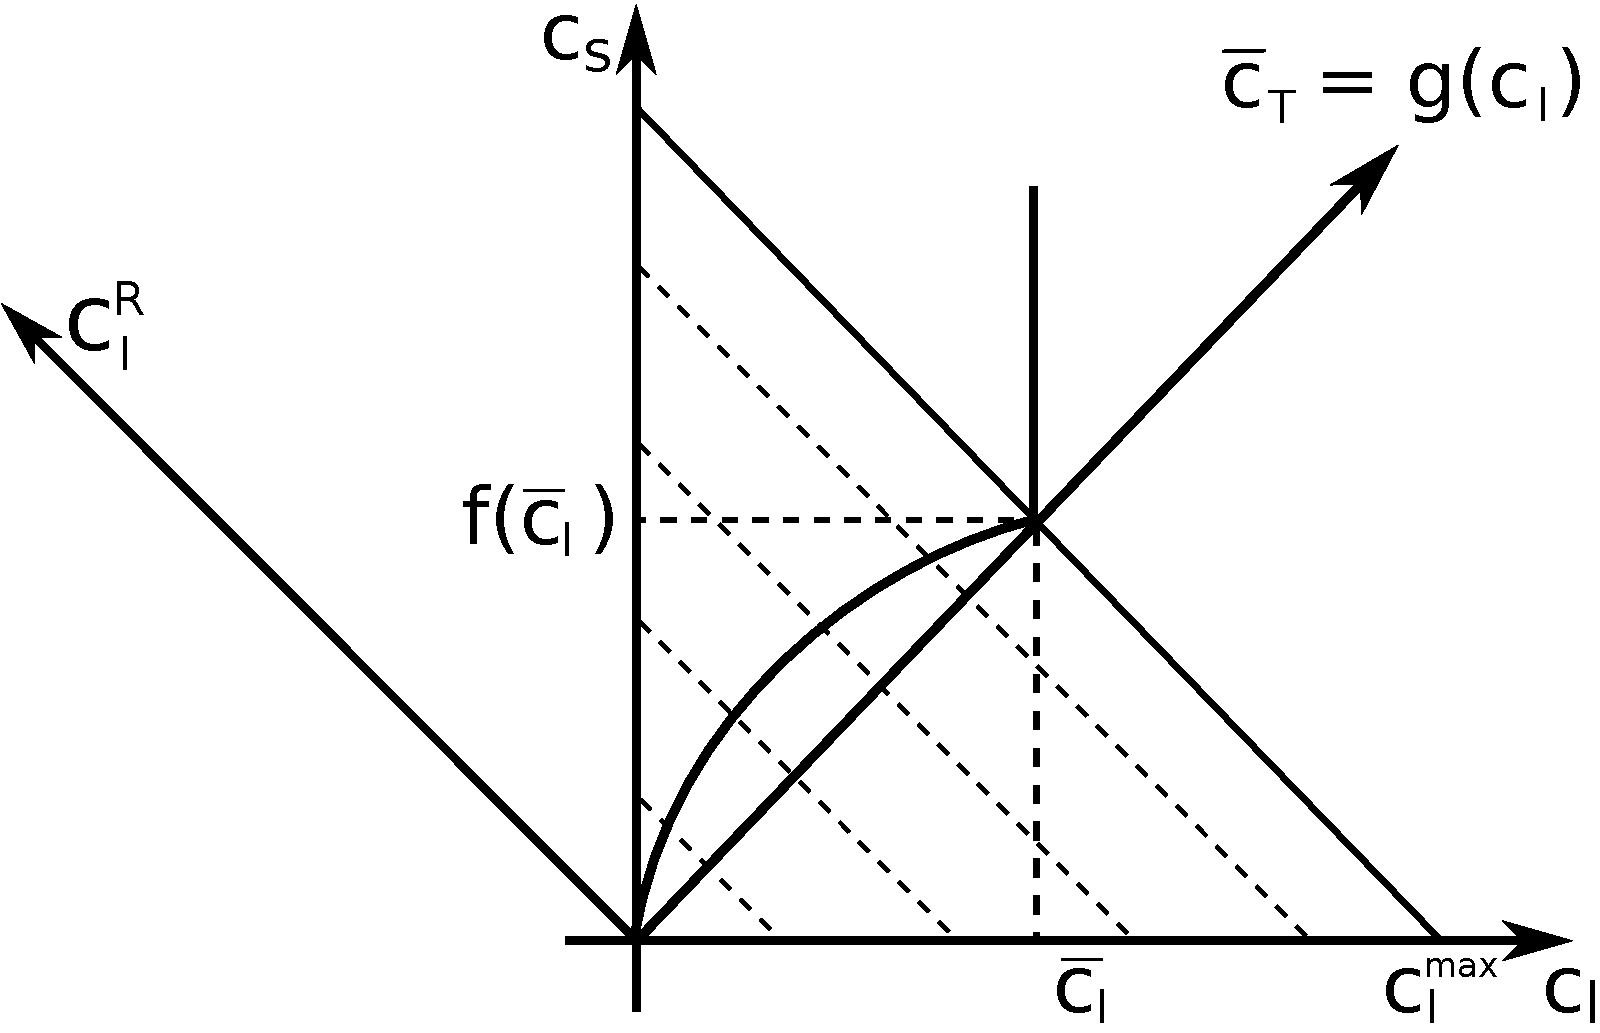
\includegraphics[width = 0.75\textwidth]{\fig/sorpce.pdf}
 \caption{Sorption in combination with limmited solubility.}
 \label{fig:sorpce}
\end{figure}


To approximate the equation \eqref{eq:nonlin_sorption} using interpolation we need to prepare the set of values 
which represent $[c_l, f(c_l)]$, with $c_l$ equidistantly distributed in transformed (rotated and rescaled) 
coordination system at first. The approach for construction of interpolation table follows.
\begin{enumerate}
 \item Maximal ``total mass'' $\bar{c}_T = \mu_l\cdot \bar{c}_l + \mu_s\cdot f(\bar{c}_l)$ is computed.
 \item Total mass step is derived $mass\_step = \bar{c}_T/n\_steps$. $n\_steps$ is given by
       \hyperA{Sorption::substeps}{$substeps$}.
 \item Appropriate $c_T^j = (mass\_step\cdot j)/\mu_l,~j\in \{0,\ldots, n\_steps\}$ are computed. 
 \item The equations $\mu_l \cdot c_T^j = \mu_l\cdot c_l^j + \mu_s\cdot f(c_l^j)~j\in \{0,\ldots, n\_steps\}$ are solved 
       for $c_l^j$ as unknowns. The solution is the set of ordered couples (points) 
       $[c_l^j,f(c_l^j)],~j\in\{0,\ldots,n\_steps\}$.
\end{enumerate}
After computation of $\{[c_l^j,f(c_l^j)]\}$ we transform these coordinates to the system where the total mass is 
an independent variable. This is done by multiplication of precomputed points using the transformation matrix ${\bf A}$:
\begin{equation}
 \begin{array}{l}
  \vec{c}\,^R = {\bf A}\cdot\vec{c}\\
  \left[\begin{array}{c} c_l^{R,j}\\ c_s^{R,j} \end{array}\right] = 
  \left[\begin{array}{cc}
    \vartheta\cdot \rho_w & M_s(1 - \vartheta)\rho_R\\
    -M_s(1 - \vartheta)\rho_R & \vartheta\cdot \rho_w
  \end{array}\right]\cdot
  \left[\begin{array}{c} c_l^j\\ c_s^j \end{array}\right]\\
  j\in\{0,\ldots,n\_steps\}
 \end{array}
 \label{eq:transf_mat}
\end{equation}

The values $c_l^{R,j}$ are equidistantly distributed and there is no reason to save them, but the values 
$c_s^{R,j}$ are stored in onedimensional interpolation table.

Once we have the interpolation table, we can use it for projection of ${[c_l,c_s]}$ transport results on the 
isotherm under consideration. The approach looks as folows.
\begin{enumerate}
 \item Achieved concentrations are transformed to the coordinate system through multiplication with the 
       matrix ${\bf A}$, see \eqref{eq:transf_mat}.
 \item Transformed values are interpolated.
 \item The result of interpolation is transformed back. The backward transformation consist of multiplication 
       with ${\bf A}^T$ which is followed by rescaling the result. Rescaling the result is necessary because  
       ${\bf A}$ is not orthonormal as it is shown bellow.
 \[
 \begin{array}{l}
 {\bf A}^T\cdot{\bf A} =
  \left((\vartheta - 1)^2\cdot M_s^2\cdot \rho_R^2 + \vartheta^2\cdot \rho_w^2\right)\cdot\left[\begin{array}{cc}
    1 & 0\\
    0 & 1
  \end{array}\right]
  \end{array}
 \]
\end{enumerate}


\subsection{Limited solubility}\label{subsec:lim_solub}
When $\mu_l\cdot c_l + \mu_s\cdot f(c_l) > \mu_l\cdot \bar{c}_l + \mu_s\cdot f(\bar{c}_l)$ neither iterative 
solver nor interpolation table is used. The aqueous concentration is set to be $\bar{c}_l$ and sorbed 
concentration is computed $c_s = (\mu_l\cdot c_l + \mu_s\cdot f(c_l) - \mu_l\cdot \bar{c}_l)/\mu_s$.

\subsection{Sorption in dual porosity model} 
\label{subsec:sorp_dual_por}
There are two parameters $\mu_l$ and $\mu_s$, scale of aqueous concentration and scale of sorbed concentration, respectively.  
There is a difference in computation of these in the dual porosity model because both work on different concentrations
and different zones.

Let $c_{ml}$ and $c_{ms}$ be concentration in liquid and in solid in the mobile zone, 
$c_{il}$ and $c_{is}$ be concentration in liquid and in solid in the immobile zone,
$\vartheta_m$ and $\vartheta_i$ be the mobile and the immobile porosity,
and $\varphi$ be the sorbing surface.

The sorbing surface in the mobile zone is given by
\begin{equation}
  \varphi = \frac{\vartheta_m}{\vartheta_m + \vartheta_i}, 
\end{equation}

while in the immobile zone it becomes
\[ 1 - \varphi = 1-\frac{\vartheta_m}{\vartheta_m + \vartheta_i} = \frac{\vartheta_i}{\vartheta_m + \vartheta_i}. \]

Remind the mass balance equation \eqref{eq:nonlin_sorption}.
In the dual porosity model, the scaling parameters $\mu_l$, $\mu_s$ are slightly different.
In particular, the mass balance in the mobile zone reads:
\begin{eqnarray}
 \begin{array}{l}
  c_T = \mu_l\cdot c_{ml} + \mu_s\cdot c_{ms},\\
  \mu_l = \varrho_l \cdot \vartheta_m, \\
  \mu_s = M_s \cdot\varrho_s\cdot(1-\vartheta_m - \vartheta_i)\varphi,
 \end{array}
 \label{eq:scale_params_m}
\end{eqnarray}
while in the immobile zone it has the form:
\begin{eqnarray}
 \begin{array}{l}
  c_T = \mu_l\cdot c_{il} + \mu_s\cdot c_{is},\\
  \mu_l = \varrho_l \cdot \vartheta_i, \\
  \mu_s = M_s \cdot\varrho_s\cdot(1-\vartheta_m - \vartheta_i)(1 - \varphi).
 \end{array}
 \label{eq:scale_params_i}
\end{eqnarray}


% TODO: Describe reactions, decays, numerical methods
%% Copyright (C) 2007 Technical University of Liberec.  All rights reserved.
%
% Please make a following refer to Flow123d on your project site if you use the program for any purpose,
% especially for academic research:
% Flow123d, Research Centre: Advanced Remedial Technologies, Technical University of Liberec, Czech Republic
%
% This program is free software; you can redistribute it and/or modify it under the terms
% of the GNU General Public License version 3 as published by the Free Software Foundation.
%
% This program is distributed in the hope that it will be useful, but WITHOUT ANY WARRANTY;
% without even the implied warranty of MERCHANTABILITY or FITNESS FOR A PARTICULAR PURPOSE.
% See the GNU General Public License for more details.
%
% You should have received a copy of the GNU General Public License along with this program; if not,
% write to the Free Software Foundation, Inc., 59 Temple Place - Suite 330, Boston, MA 021110-1307, USA.

\normalsize

\subsection{Linear Reactions}
\label{sec:linear_reactions}
The software suppports linear chemical reactions in the transport operator splitting method. 
The linear chemical reactions (we will recall them only as 'reactions' in this section) can desribe
\begin{itemize}
  \item first order kinetic chemical reactions
  \item radioactive decays, their chains and also complex chains with branches.
\end{itemize}
In the first case, the kinetics of a reaction is determined by a kinetic constant \hyperA{Substep::kinetic}{$k$}. 
In the second case, the radioactive decay is determined by the half life of the reactant 
\hyperA{Substep::half-life}{$t_{1/2}$}. Both notations
%
\[ A\xrightarrow{k} B, \qquad A\xrightarrow{t_{1/2}} B \]
%
express the same reaction and are governed by the same first order differential equation 
%
\[ \frac{\d c_A}{\d\tau} = -kc_A = - \frac{\ln 2}{t_{1/2}}\, c_A. \]
%
The relation between $k$ and $t_{1/2}$ is derived below
\begin{eqnarray*}
    \frac{\d c_A}{\d\tau} &=& -k c_A\\
    \frac{\d c_A}{c_A} &=& -k \d\tau\\
    \int\limits_{c_A^0}^{c_A^0/2}\frac{\d c_A}{c_A} &=& -k\int\limits_{0}^{t_{1/2}} 1\d\tau\\
    \big[ \ln c_A\big]^{c_A^0/2}_{c_A^0} &=& -\big[k\tau\big]^{t_{1/2}}_{0}\\
    \ln\frac{c_A^0}{2} - \ln c_A^0 &=& - k t_{1/2}\\
    \ln 2 &=& k t_{1/2}\\
    k &=& \frac{\ln 2}{t_{1/2}}.
\end{eqnarray*}



Lets consider to have a narrow decay chain without branches. This kind of decay chain can be described by following equation
\[
 A\xrightarrow{t_{1/2,A}}B\xrightarrow{t_{1/2,B}}C\xrightarrow{t_{1/2,C}}D\xrightarrow{t_{1/2,D}}E,
\]
where letters $\{A,\ldots, E\}$ denotes isotopes contained in considered decay chain and ${t_{1/2},i},~i\in\{A,\ldots, E\}$ is a symbol for a half-life of $i$-th isotope.
For a simulation of radioactive decay and first order reactions matrix multiplication based approach has been developed. It has been based on an arrangement of all the data to matrices. The matrix ${\bf C}^k$ contains the information about concentrations of all species ($s$) in all observed elements ($e$). The upper index $k$ denotes $k$-th time step. The matrix ${\bf C}^k$ has the dimension $e\times s~( rows \times columns)$.
The transport simulation is realized by matrix multiplication 
\[
  {\bf T}\cdot{\bf C}^k = {\bf C}^{k+1},
\]
where ${\bf T}$ is a square, block-diagonal matrix, representing a set of algebraic equations constructed from a set of partial differential equations.
When the simulation of the radioactive decay or the first order reaction is switched on, one step of
simulation changes to 
\[
  {\bf T}\cdot{\bf C}^k\cdot{\bf R} = {\bf C}^{k+1},
\]
where ${\bf R}$ is a square matrix with the dimension $(s \times s)$ . It is much easier to construct and to use ${\bf R}$ , than to include chemical influence to the transport
matrix ${\bf T}$ , because the matrix ${\bf R}$ has usually a simple structure and $s$ is much smaller than $e$. In the most simple case, when the order of identification numbers of isotopes in considered decay chain is the same as the order of identifiers of species transported by groundwater, then just two
diagonals are engaged and the matrix R looks as follows:

\begin{tiny}\[
   \begin{array}{l}
    {\bf R} = \left(
    \begin{array}{cccccc}
     \left(\frac{1}{2}\right)^\frac{\Delta t}{t_{1/2,1}} & 1 - \left(\frac{1}{2}\right)^\frac{\Delta t}{t_{1/2,i}} & 0 & \hdots & \hdots & 0\\
     0 & \left(\frac{1}{2}\right)^\frac{\Delta t}{t_{1/2,2}} & 1 - \left(\frac{1}{2}\right)^\frac{\Delta t}{t_{1/2,2}} & 0 & \ddots & 0 \\
     \vdots & \ddots & \ddots & \ddots & \ddots & \vdots\\
     0 & \ddots & 0 & \left(\frac{1}{2}\right)^\frac{\Delta t}{t_{1/2,n-2}} & 1 - \left(\frac{1}{2}\right)^\frac{\Delta t}{t_{1/2,n-2}} & 0 \\
     0 & \hdots & \hdots & 0 & \left(\frac{1}{2}\right)^\frac{\Delta t}{t_{1/2,n-1}} & 1 - \left(\frac{1}{2}\right)^\frac{\Delta t}{t_{1/2,n-1}}\\
     0 & \hdots & \hdots & 0 & 0 & 1
    \end{array}\right)
   \end{array}
\]\end{tiny}

Every single $j$-th column, except the first one, includes the contribution $1 - \left(\frac{1}{2}\right)^\frac{\Delta t}{t_{1/2,j}},~j\in\{A,\ldots, E\}$ from $(j-1)$-th
isotope with its half-life $t_{1/2,j-1}$. The term $\left(\frac{1}{2}\right)^\frac{\Delta t}{t_{1/2,j}}$ describes concentration decrease caused by the radioactive decay of $j$-th isotope itself. In general cases the matrix ${\bf R}$ can have much more complicated structure, especially when the considered decay chain has more branches.
The implementation of the radioactive decay in Flow123D does not firmly include standard natural decay chain. Instead of that it is possible for a user to define his/her decay chain.

It is also possible to simulate decay chains with branches as picture \ref{pic:dec_branches} shows.

\begin{figure}[htb]
 \centering
 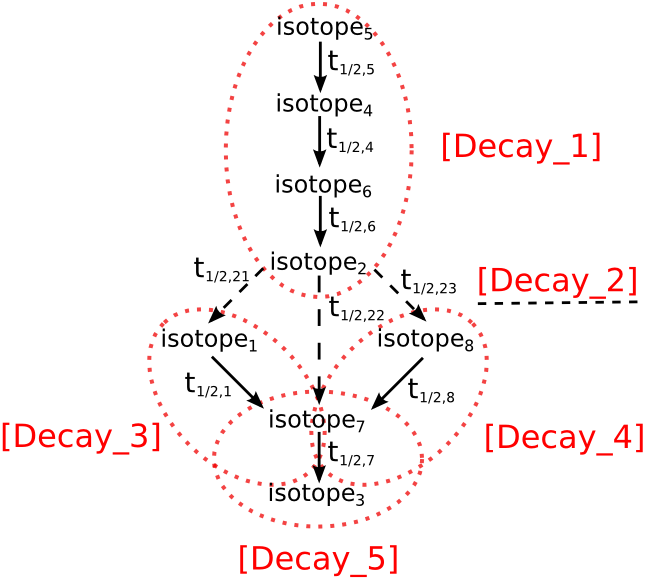
\includegraphics[width = 8cm]{\fig /decay_chain.png}
 \caption{Decay chain with branches.}
 \label{pic:dec_branches}
\end{figure}


When it comes to a simulation of first order reactions, the kinetic constant is given as an input. 
The description of a kinetic chemical reaction has obviously two folowing forms
\[
  \begin{array}{l}
    A\xrightarrow{k}B,\\
    \frac{dc^A}{dt} = -k \cdot c^A.
  \end{array}
\]
The first one description is a standard chemical one. The second equation describes temporal decrease in amount of concentrations of the specie $c^A$. The constant $k$ is so called kinetic constant and for the case of a first order reactions it is equal to so called reaction rate. The order of reaction with just one reactant is equal to the power of $c^A$ in partial diferential reaction.

For an inclusion of first order reaction into a reaction matrix a half-life needs to be computed from the corresponding kinetic constant $k$. The derivation follows
\[
  \begin{array}{l}
    A\xrightarrow{k} B\\
    \frac{dc^A}{d\tau} = -k\cdot c_A\\
    \frac{dc^A}{c^A} = -k\cdot d\tau\\
    \int\limits_{c^A_0/2}^{c^A_0}\frac{dc^A}{c^A} = -k\cdot\int\limits_{t_{1/2,A}}^{0} d\tau\\
    \left[ ln c^A\right]_{c^A_0/2}^{c^A_0} = -[k\tau]_{t_{1/2,A}}^{0}\\
    ln c^A_0 - \ln\frac{c^A_0}{2} = k\cdot t_{1/2,A}\\
%     c^A (t) = c^A_0\cdot e^{-k\cdot t_{1/2,A}}\\
%     {\bf substitution} \qquad c^A(t_{1/2,A}) = \frac{1}{2}\cdot c^A_0\\
%     \frac{1}{2} c^A_0 = c^A_0\cdot e^{-k_1\cdot t_{1/2,A}}\\
    \ln 2 = k \cdot t_{1/2,A}\\
    t_{1/2,A} = \frac{ln 2}{k}
  \end{array}                                                                                                                                                                                                                                                                                                            
\]
The matrix ${\bf R}$ is constructed in the same way as for the radioactive
decay.


\section{Heat Transfer}

Under the assumption of thermal equilibrium between the solid and liquid phase, the energy balance equation has the form\footnote{For lower dimensions this form can be derived as in Section \ref{sc:ad_on_fractures} using $w:=\delta\tilde s T$, $u:=T$, $\tn A:=\delta\lambda\tn I$, $\vc b:=\frac{\varrho_l c_l}{\tilde s}\vc w$.}
\[
    \partial_t\left(\delta \tilde s T \right) + \div(\varrho_l c_l T \vc q) - \div(\delta\Lambda\nabla T) = F^T + F^T_C.
\]
The principal unknown is the temperature $T$ [K].
Other quantities are:
\begin{itemize}
\item \hyperA{HeatTransfer-DG-Data::fluid-density}{$\varrho_l$}, \hyperA{HeatTransfer-DG-Data::solid-density}{$\varrho_s$} \units{1}{-3}{} is the density of the fluid and solid phase, respectively.
\item \hyperA{HeatTransfer-DG-Data::fluid-heat-capacity}{$c_l$}, \hyperA{HeatTransfer-DG-Data::solid-heat-capacity}{$c_s$} [J$\mathrm{kg}^{-1}\mathrm{K}^{-1}$] is the heat capacity of fluid and solid phase, respectively.
\item $\tilde s$ [J$\mathrm{m}^{-3}\mathrm{K}^{-1}$] is the volumetric heat capacity of the porous medium defined as
\[ \tilde s = \hyperA{HeatTransfer-DG-Data::porosity}{\th}\varrho_l c_l + (1-\th)\varrho_s c_s. \]
\item $\Lambda$ [W$\mathrm{m}^{-1}\mathrm{K}^{-1}$] is the thermal dispersion tensor:
\[ \Lambda = \Lambda^{cond} + \Lambda^{disp} \]
\[ \Lambda^{cond} = \left(\th \lambda_l^{cond} + (1-\th)\lambda_s^{cond}\right)\tn I, \]
\[ \Lambda^{disp} = \th \varrho_l c_l|\vc v|\left(\alpha_T\tn I + (\alpha_L-\alpha_T)\frac{\vc v\otimes\vc v}{|\vc v|^2}\right), \]
where \hyperA{HeatTransfer-DG-Data::fluid-heat-conductivity}{$\lambda_l^{cond}$}, \hyperA{HeatTransfer-DG-Data::solid-heat-conductivity}{$\lambda_s^{cond}$} [W$\mathrm{m}^{-1}\mathrm{K}^{-1}$] is the thermal conductivity of the fluid and solid phase, respectively, and \hyperA{HeatTransfer-DG-Data::disp-l}{$\alpha_L$}, \hyperA{HeatTransfer-DG-Data::disp-t}{$\alpha_T$} \units{}{1}{} is the longitudal and transverse dispersivity in the fluid.

\item $F^T$ [J$\mathrm{m}^{-d}\mathrm{s}^{-1}$] represents the thermal source:
\[ F^T = \delta \th F^T_l + \delta (1-\th) F^T_s, \]
\[ F^T_l = f_l^T + \varrho_l c_l \sigma^T_l(T-T_l), \]
\[ F^T_s = f_s^T + \varrho_s c_s \sigma^T_s(T-T_s), \]
where \hyperA{HeatTransfer-DG-Data::fluid-thermal-source}{$f_l^T$}, \hyperA{HeatTransfer-DG-Data::solid-thermal-source}{$f_s^T$} [W$\mathrm{m}^{-3}$] is the density of thermal sources in fluid and solid, respectively, \hyperA{HeatTransfer-DG-Data::fluid-ref-temperature}{$T_l$}, \hyperA{HeatTransfer-DG-Data::solid-ref-temperature}{$T_s$} [K] is a reference temperature and \hyperA{HeatTransfer-DG-Data::fluid-heat-exchange-rate}{$\sigma^T_l$}, \hyperA{HeatTransfer-DG-Data::solid-heat-exchange-rate}{$\sigma^T_s$} \units{}{}{-1} is the heat exchange rate.
\end{itemize}



\paragraph{Initial and boundary conditions.}
At time $t=0$ the temperature is determined by the initial condition
$$ T(0,\vc x) = \hyperA{HeatTransfer-DG-Data::init-temperature}{T_0}(\vc x). $$
Given the decomposition of $\partial\Omega_d$ into $\Gamma_I\cup\Gamma_D\cup\Gamma_N\cup\Gamma_R$ (see Section \ref{sc:transport_model}), we prescribe the following boundary conditions:
\begin{itemize}
\item Dirichlet:
\[ T = \hyperA{HeatTransfer-DG-Data::bc-temperature}{T_D} \mbox{ on }\Gamma_I^+\cup\Gamma_D, \]
\item Homogeneous Neumann:
\[ \left(\varrho_l c_l T \vc q - \delta\Lambda\nabla T\right)\cdot\vc n = 0 \mbox{ on }\Gamma_I^-, \]
\item Neumann:
\[ \left(\varrho_l c_l T \vc q - \delta\Lambda\nabla T\right)\cdot\vc n = \hyperA{HeatTransfer-DG-Data::bc-flux}{f_N} \mbox{ on }\Gamma_N, \]
\item Robin (Newton):
\[ \left(\varrho_l c_l T \vc q - \delta\Lambda\nabla T\right)\cdot\vc n = \hyperA{HeatTransfer-DG-Data::bc-robin-sigma}{\sigma_R}(T-\hyperA{HeatTransfer-DG-Data::bc-temperature}{T_D}) \mbox{ on }\Gamma_R. \]
\end{itemize}






\paragraph{Communication between dimensions.}
Denoting $T_{d+1}$, $T_d$ the temperature in $\Omega_{d+1}$ and $\Omega_d$, respectively, the communication on the interface between $\Omega_{d+1}$ and $\Omega_d$ is described by the quantity
\begin{equation}
  \label{e:inter_dim_flux_heat}
  q^T_{d+1,d} = \sigma^T_{d+1,d} \frac{\delta_{d+1}^2}{\delta_d}2\Lambda_d:\n\otimes\n ( T_{d+1} - T_d) + \begin{cases} \varrho_l c_l q^l_{d+1,d} T_{d+1} & \mbox{ if }q^l_{d+1,d}\ge 0,\\\varrho_l c_l q^l_{d+1,d} \frac{\tilde s_d}{\tilde s_{d+1}} T_d & \mbox{ if } q^l_{d+1,d}<0,\end{cases}
\end{equation}
where
\begin{itemize}
\item $q^T_{d+1,d}$ [W$\mathrm{m}^{-2}$] is the density of heat flux from $\Omega_{d+1}$ to $\Omega_d$,
\item \hyperA{HeatTransfer-DG-Data::fracture-sigma}{$\sigma^T_{d+1,d}$} \units{}{}{} is a transition parameter.
Its value determines the exchange of energy between dimensions due to temperature difference.
In general, it is recommended to leave the default value $\sigma^T=1$ or to set $\sigma^T=0$ (when exchange is due to water flux only).
\item $q^l_{d+1,d}=\vc q_{d+1}\cdot\vc n$ is the water flux from $\Omega_{d+1}$ to $\Omega_d$.
\end{itemize}
The communication between dimensions is incorporated as the total flux boundary condition for the problem on $\Omega_{d+1}$:
\begin{equation}
\label{e:heat_FC}
\left(\varrho_l c_l T \vc q - \delta\Lambda\nabla T\right)\cdot\vc n = q^T
\end{equation}
and a source term in $\Omega_d$:
\begin{equation}
F^T_{C3} = 0,\quad
F^T_{C2} = q^T_{32},\quad
F^T_{C1} = q^T_{21}.
\end{equation}




\paragraph{Energy balance.}
The heat equation satisfies the balance of energy in the following form:
$$ e(0) + \int_0^t s(\tau) \,d\tau - \int_0^t f(\tau) \,d\tau = e(t) $$
for any instant $t$ in the computational time interval.
Here
$$ e(t) := \sum_{d=1}^3\int_{\Omega^d}(\delta \tilde s T)(t,\vc x)\,d\vc x, $$
$$ s(t) := \sum_{d=1}^3\int_{\Omega^d}F_S^T(t,\vc x)\,d\vc x, $$
$$ f(t) := \sum_{d=1}^3\int_{\partial\Omega^d}\left(\varrho_l c_l T\vc q - \delta\Lambda\nabla T\right)(t,\vc x)\cdot\vc n \,d\vc x $$
is the energy [J], the volume source [J$\mathrm{s}^{-1}$] and the energy flux [J$\mathrm{s}^{-1}$] at time $t$, respectively.
The energy, flux and source on every geometrical region is calculated at each computational time step and the values together with the control sums are written to the file \texttt{mass\_balance.txt}.







% TODO: Update numerical topics
% \input{numerical}



%\input{semchem}


\chapter{File Formats}
\label{chapter:file-formats}
%\section{Input format}

In this chapter, we shall describe structure of the main input file and data formats of other input files.
In particular we briefly describe the GMSH file format used for both the computational mesh as well as for the input of general spatial data.


\section{Main Input File}
\label{sec:CONformat}

In this section, we shall describe structure of the main input file that is given either as the first positional argument or through 
the parameter \verb'-s' on the command line. First, we provide a~quick introduction to the YAML file format. Then, we demonstrate the most important 
input structures on the examples. 







\subsection{YAML basics}
YAML is a~human readable data format. It is designed to be both human readable and human editable. As it is not a~markup languages, there are
no tags to determine type of the data. The indentation and justification is used instead for data organization. Moreover the used YAML format (version 1.2) is 
superset of the JSON format, another minimalist data serialization format where braces and brackets are used instead of indentation.
For the more detailed description see \href{https://en.wikipedia.org/wiki/YAML}{Wikipedia} 
for further technical details and for reference parsers for various programming languages see YAML \href{http://yaml.org/}{home page} .

\subsubsection{Hierarchy of Mappings and Lists}
Elementary data are organized to lists and mappings. Let us start with an example of a~list:
\begin{verbatim}
# Example of list 
- 3.14                  # a number
- 2014-01-14            # a date
- Simple string.        # a string
- "3 is three"          # quoting necessary
- '3 is three'          # other quoting
- true                  # boolean
\end{verbatim}
Comments are started by a~hash (\verb'#') which can appear anywhere on a~line and marks the comment up to the end of line.
The the list follows with single item per line preceded by a~dash (\verb'-'). Any value starting by a~digit is interpreted as a~number
or date. Values starting with letter is interpreted as a~string. Otherwise one may use double (\verb'""') or single (\verb"''") 
quotas to mark a~string value explicitly. Finally some strings are interpreted as Boolean values, it is recommended to use 
\verb'true' and \verb'false' (other possible pairs are e.g. \verb'yes/no', \verb'y/n', \verb'on/off'). 

Alternatively a~list may be written in compact "JSON" way enclosing the list into brackets:
\begin{verbatim}
# Compact list
[ 3.14, 2014-01-14, Simple string.,
"3 is three", '3 is three'] 
\end{verbatim}

Other data structure is called mapping, which is also known as directory or associative array:
\begin{verbatim}
# Example of a mapping
pi: 3.14
date: 2014-01-14   
name: Mr. Simple String
\end{verbatim}

Again one may use also JSON syntax with mapping enclosed in braces:
\begin{verbatim}
# Compact mapping
{ pi: 3.14, date: 2014-01-14,   
name: Mr. Simple String }
\end{verbatim}

Mappings and lists may by mutually nested:
\begin{verbatim}
list:
    - one
    - two
    - 
        - three one 
        - three two
map:
    a: one 
    b: two
\end{verbatim}

A string may be split to more lines using {\it greater then} (\verb'>') and multi-line strings may be entered after {\it vertical line} (\verb'|'):
\begin{verbatim}
# single long string
one_line: >
    Single line string
    broken into two lines.
# multi line string
multi_line: |
    First line.
    Second line.
\end{verbatim}
In the first case the line breaks are replaced by space, in the second case the line breaks are preserved.
In both cases the leading indentation is removed.


\subsubsection{Tags}
YAML format defines a~syntax for explicit specification of types of values including the types specific to an application.
The application specific tags are used by Flow123d to specify particular implementation of various algorithms or data types.
The general syntax of tags is quite complicated, so we present only the syntax used in the Flow123d input.
\begin{verbatim}
    field_a: !FieldFormula
        value: !!str "5 * x" 
    field_b:  !FieldFormula "5 * x"   
\end{verbatim}

The \verb'field_a' have specified evaluation algorithm \verb'FieldFormula', the key value have explicitly specified the default tag \verb'str'.
Note that default types are detected automatically and need not to be specified. On the third line we use even more compact way to 
express the same thing. Further details about usage of tags in Flow123d follows in Section \ref{sec:abstract}.

\subsubsection{References}
Anchors and references allows to reduce redundancy in the input data:
\begin{verbatim}
aux_name: &anchor_name John Smith
aux_man: &common_man
    sex: man
    city: Prague
    
people:
   - << *_common_man
     name: John Paul
   - << *_common_man
     name: *anchor_name
\end{verbatim}
On the first line, we define the anchor \verb'&anchor_name' for the value \verb'John Smith'. On the second line, 
we define the anchor \verb'&common_man' for the dictionary. Later, we use \verb'<<' to inject the dictionary 
referenced by \verb'*common_man'. Finally the anchor \verb'&anchor_name' is referenced by \verb'*anchor_name' to reuse the 
name \verb'John Smith'.

Ignoring the auxiliary keys \verb'aux_name' and \verb'aux_man' this is equivalent to:
\begin{verbatim}
people:
   - sex: man
     city: Prague
     name: John Paul
   - sex: man
     city: Prague
     name: John Smith
\end{verbatim}


\subsubsection{Gotchas}
\begin{itemize}
 \item Unquoted string values can not contain characters: colon \verb':', hash \verb'#', 
 brackets \verb'[]', braces \verb'{}', less then \verb'<', vertical bar \verb'|'.
 \item For indentation one can use only spaces; tabs are not allowed. However, your editor may automatically convert tabs to spaces.
 \item Boolean special strings must be quoted if you want to express a~string. This is not problem for the Flow123d input.
 \item Numbers starting with digit zero are interpreted as octal numbers. 
\end{itemize}

\subsection{Flow123d input types}
\label{sec:input_types}
Flow123d have a~subsystem for definition of the structure of the input file including preliminary checks for the 
correctness of the values. This subsystem works with elementary data types:
\begin{itemize}
 \item {\it Bool} corresponds to the YAML Boolean values
 \item {\it Double}, {\it Integer} initialized from YAML numeric values. 
 \item {\it String}, {\it FileName}, {\it Selections} initialized from YAML strings.
\end{itemize}
Numerical values have defined valid ranges. FileName values are used for reference to external files either for input or for output.
Selection type defines a~finite number of valid string values which may appear on the input. 
These elementary types are further organized into Records and Arrays in order to specify strongly typed definition of the 
input data file. Array and Records forms so called input structure tree (IST).

In order to make {\it "simple things simple and complex things possible" (Alan Kay)} the input system provides
so called {\it automatic conversions}. If the YAML type on input does not match the expected data type automatic conversion tries to convert 
the input to the expected type. Automatic conversion rules for individual composed types follows.

\subsubsection{Record (YAML Mapping, JSON object)}
A Record is initialized from the YAML mapping. However, in contrast to YAML mappings 
the Records have fixed keys with fixed types. 
This is natural as Records are used for initialization of C++ objects which 
are also strongly typed. Every Record type have unique name and have defined list of its keys.
Keys are lowercase strings without spaces, possibly using digits and underscore. Every key has
a type and default value specification. Default value specification can be:
\begin{description} 
 \item[obligatory] --- means no default value, which has to be specified at input. 
 \item[optional] --- means no default value, but value is needs not to be specified. Unspecified value usually means that you turn off some functionality.
 \item[default at declaration] --- the default value is explicitly given in declaration and is automatically provided by the input subsystem if needed
 \item[default at read time] --- the default value is provided at read time, usually from some other variable. In the documentation, 
 there is only textual description where the default value comes from.
\end{description}

Records that have all keys with default value or optional safe the single key $K$ may support autoconversion from an input of the type that match 
the type of the key $K$. For example:
\begin{verbatim}
  mesh: "mesh_file.msh"
\end{verbatim}
is converted to:
\begin{verbatim}
  mesh:
    mesh_file: "mesh_file.msh"
    regions: null
    partitioning: any_neighboring
    print_regions: false
    intersection_search: BIHsearch
\end{verbatim}
with the key \verb'regions' being optional and the last three keys having its default values. 


\subsubsection{Array (YAML List, JSON array)}
An Array is initialized from a~YAML list. But, in opposition to the YAML mapping, the values in a~single Array 
have all the same type. So the particular Array type is given by the type of its elements and a~specification of its size range.

Automatic conversion performs kind of transposition of the data. It simplifies input of the list of records (or arrays) 
with redundant structure, e.g. consider input
\begin{verbatim}
  list:
    a: [1,2)
    b: 4
    c: [5,6]
\end{verbatim}
Assuming that key \verb'list' have the type Array of Records and keys \verb'a', \verb'b', \verb'c' are all numerical scalars this input is equivalent to
\begin{verbatim}
  list:
    - a: 1
      b: 4
      c: 5
    - a: 2
      b: 4
      c: 6
\end{verbatim}
The rule works as follows, if a~key $K$ should have type Array, but some other type is on the input, 
we search through the input under the key $K$ for all Arrays $S$ standing instead of scalars.
All these arrays must have the same length $n$. Then the $i$-th element of the key $A$ array is
copy of the input keeping only $i$-th elements of the Arrays $S$.
As a~special case if there are no Arrays $S$ a~list with single element equal to the input is created.
Only this simplest conversion to an Array is applied if inappropriate type is found 
while the transposition is processed.





\subsubsection{Abstract}
\label{sec:abstract}
An Abstract type allows a~certain kind of polymorphism corresponding to a~pure abstract class in C++ or to an interface in Java. 
Every Abstract type have unique name and set of Records that implements the Abstract. The particular type must be provided on input through the YAML tag.
See description of \hyperlink{sec:Fields}{Fields} below for examples.

An Abstract type may have specified the default implementation. If this default Record supports automatic conversion from one of its keys
we can see it as an automatic conversion from that key to the Abstract. For example
\begin{verbatim}
 conductivity: 2.0
\end{verbatim}
where conductivity is of Abstract type \verb'Field' with scalar values, is in fact converted to
\begin{verbatim}
 conductivity: !FieldConstant
    value: 2.0
\end{verbatim}
as the \verb'FieldConstant' is default implementation of the field and it is auto=convertible from the key \verb'value'. 

\subsubsection{Flow123d specific tags}
\label{sec:spec_tags}
Currently just two specific tags are implemented, both allowing inclusion of data in other files.

{\bf Include other YAML file} The tag \verb'!include' can be used to read a~key value from other YAML file.
Path to the file is specified as the value of the key. A relative path is rooted in the folder of the main input file.
A particular type of an Abstract key is specified as a~composed tag \verb'!include,<TYPE>'.

Example, the main input file:
\begin{verbatim}
    flow123d_version: 2.0.0
    problem: !Coupling_Sequential
        description: Test8 - Steady flow with sources
        mesh:
            mesh_file: ../00_mesh/square_1x1_shift.msh
        flow_equation: !include,Flow_Darcy_MH
            input_darcy.yaml
\end{verbatim}
Content of \verb'input_darcy.yaml', included Record:
\begin{verbatim}
    nonlinear_solver:
        linear_solver: !Petsc
    input_fields:
        darcy_input_fields.yaml
    balance: {}
    output_stream: 
        file: ./flow.pvd
\end{verbatim}
Content of \verb'darcy_input_fields.yaml', included Array:
\begin{verbatim}
    - region: plane
        anisotropy: 1
        water_source_density: !FieldFormula
        value: 2*(1-x^2)+2*(1-y^2)
    - region: .plane_boundary
        bc_type: dirichlet
        bc_pressure: 0    
\end{verbatim}

{\bf Include general CSV data}
The custom tag \verb'include_csv' can be used to include a~table (e.g. coma separated values, CSV file) as an Array of Records. 
Every line of the input table is converted to a~single element of the Array.
The tag is followed by a~Record with several keys to specify format of the data:
\begin{description}
  \item {\bf\verb'file'} \\A valid path to a~text data file. Relative to the main input file.
  \item {\bf\verb'separator'}\\ A string of characters used as separators of the values on the single line (default is coma ",").
  Tab and space are always added. Double quotas can be used to express string values containing separators, 
  backslash can be used to escaping any character with special meaning. Consecutive row of separators is interpreted as a~single separator. 
  \item {\bf\verb'n_head_lines'}\\ Skip given number of lines at the beginning.
  \item {\bf\verb'format'}\\ An input structure of a~single element in the resulting array. Type of Abstracts must be same through 
  the whole resulting Array. String scalar values with a~placeholder \verb"'$<column>'" will be replaced by the value 
  at corresponding column in the input file.
\end{description}

Current implementation have substantial limitation as it can not be combined with auto conversions. This makes these includes
little bit verbose. For example consider this section from a~main input file:
\begin{verbatim}
    ...
    substances: [A, B]
    ...    
    input_fields:
    - region: A
      porosity: !FieldTimeFunction
        time_function: !include_csv
          values:
            file: data.txt  
            separator: " "
            n_head_lines: 1
            format: 
              time: #0
              value: #1
              
    - region: .boundary_A        
      bc_conc: 
        - !FieldTimeFunction    # Substance A
          time_function: !include_csv
            values:
              file: data.txt  
              separator: " "
              n_head_lines: 1
              format: 
                time: #0
                value: #2
        - !FieldTimeFunction    # Substance B
          time_function: !include_csv
            values:
              file: data.txt  
              separator: " "
              n_head_lines: 1
              format: 
                time: #0
                value: #3
\end{verbatim}
Content of \verb'data.txt':
\begin{verbatim}
time    porosity        bc_conc_X     bc_conc_Y
0.0     0.01            1.0           0.6
0.1     0.015           0.9           0.5
0.2     0.03            0.8           0.4
\end{verbatim}

This together will be equivalent to:
\begin{verbatim}
    input_fields:
    - region: A
      porosity: !FieldTimeFunction
        time_function: 
          - time: 0.0
            value: 0.01
          - time: 0.1
            value: 0.015
          - time: 0.2
            value: 0.03
           
    - region: .boundary_A        
      bc_conc: !FieldTimeFunction
        time_function: 
          - time: 0.0
            value: [ 1.0, 0.6]
          - time: 0.1
            value: [ 0.9, 0.5]
          - time:  0.2
            value: [ 0.8, 0.4]
\end{verbatim}

So in this particular case it would be simpler to write data directly into the main file. The include from 
the text table is efficient for the long time series.




\subsection{Input subsystem}
This section provides some implementation details about the Flow123d input subsystem. This may be helpful to better understand behavior of the program for 
some special input constructions.

\begin{figure}[!hb]
 \begin{center}
 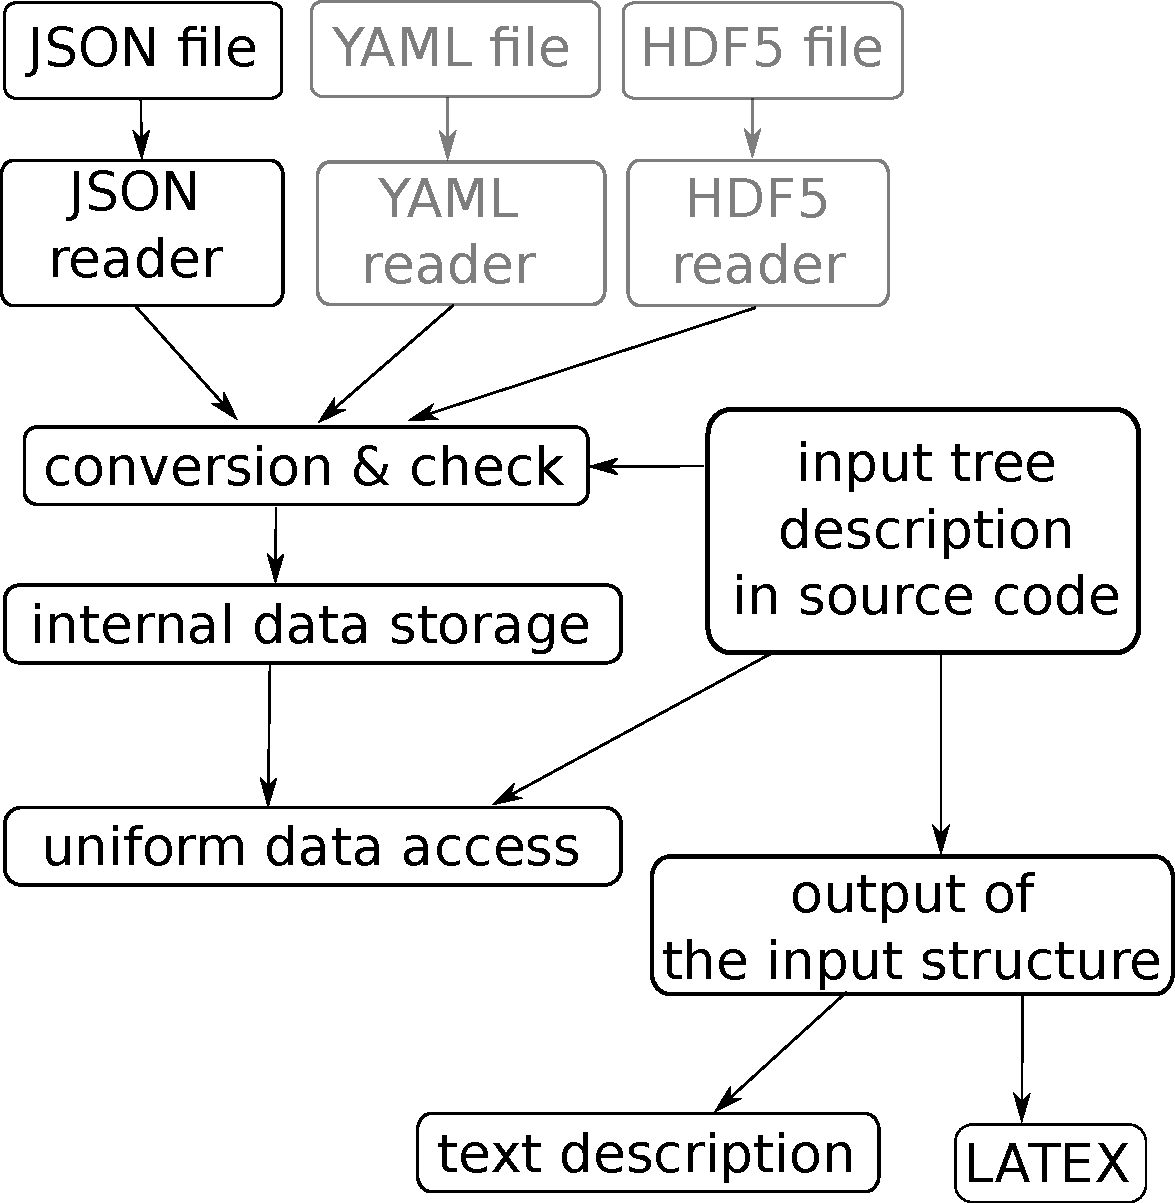
\includegraphics[scale=0.4]{\fig/input_subsystem.pdf}
 % input_subsystem.pdf: 0x0 pixel, -2147483648dpi, 0.00x0.00 cm, bb=
 \caption{Structure of the input subsystem. HDF5 format not yet supported.}
 \label{fig:input_subsystem}
 \end{center}
\end{figure}

The input subsystem of Flow123d is designed with the aim to provide uniform initialization of 
C++ classes and data structures. The scheme of the input is depicted on Figure \ref{fig:input_subsystem}.
The structure of the input file is described by the Input Structure Tree (IST) consisting of the input objects describing 
the types discussed in the previous Section \ref{sec:input_types}. The structure of the tree mostly follows follows the structure of the computational classes.

When reading the input file, the file is first parsed by the specific format parser. Using a~common interface to the parsed data, the 
structure of the data is checked against the IST and the data are pushed into the storage tree. If the input data and IST do not match
the automatic conversions described above are applied, where appropriate.
An accessor object to the root data record is the result of the file reading. The data can be retrieved through the 
accessors which combine raw data of the storage with their meaning described in IST. The IST can be written out in the JSON format
providing the description of the input file structure. This IST file is used both for generation of the input reference in HTML and \LaTeX
formats and for the Model editor --- specialized editor for the input file that is part of the GeoMop tools currently in development.

While the recommended format of the input file is YAML the JSON format can be used as well. This may be useful in particular if the input file
should be machine generated. Although the JSON format is technically subset of the YAML format. We use separate parser and use special keys in order to
mimic tags and references supported by the YAML. The type of an abstract is specified by the key \verb'TYPE'. A reference is given by a~record with the only key 
\verb'REF' which contains a~string specifying the address of the value that should be substituted.



\section{Important Record Types of Flow123d Input}
Complete description of the input structure tree can be generated into HTML or LaTeX format. While the former one provides better interactivity 
through the hyperlinks the later one is part of this user manual. The generated documentation provides whole details for all keys, but 
it may be difficult to understand the concept of the input structures. This section is aimed to provide this higher level picture.

\subsection{Mesh Record}
\label{sec:Mesh}
The \hyperA{IT::Mesh}{mesh record} provides initialization of the computational mesh consisting of points, lines, triangles and tetrahedrons in the 3D ambient space.
Currently, we support only GMSH mesh file format \href{http://geuz.org/gmsh/doc/texinfo/gmsh.html#MSH-ASCII-file-format}{MSH ASCII}. 
The input file is provided by the key \hyperA{Mesh::mesh-file}{{\tt mesh\_file}}. The file format allows to group elements into {\it regions} 
identified by a~unique label (or by ID number). The regions with labels starting with the dot character are treated as {\it boundary regions}. 
Their elements are removed from the computational domain, however they can be used to specify boundary
conditions. Other regions are called {\it bulk regions}. Every element lies directly in just one {\it simple region} while the simple regions may be 
grouped into composed regions called also region sets. A simple region may be part of any number of composed regions.
Initial assignment of the simple regions to the elements is given by the physical groups of the input GMSH file. Further
modification of this assignment as well as creation of new simple or composed regions can be done 
through the list of operations under the key \hyperA{Mesh::regions}{{\tt regions}}. The operations are performed in the order given by the input.
Operation \hyperA{IT::From-Id}{{\tt From\_Id}} sets the name of a~simple region having only ID in the input GMSH file. Operation 
\hyperA{IT::From-Label}{{\tt From\_Label}} can rename a~simple region. Operation \hyperA{IT::From-Elements}{{\tt From\_Elements}}
assign new simple region to the given list of elements overwriting their region given by the input mesh file. Finally operations 
\hyperA{IT::Union}{{\tt Union}}, \hyperA{IT::Difference}{{\tt Difference}} and \hyperA{IT::Intersection}{{\tt Intersection}}
implements standard set operations with both simple and complex regions resulting in new composed regions.




\subsection{Input Fields}
Input of every equation contains the key \verb'input_fields' used consistently for the input of the equation parameters 
in form of general time--space dependent fields.  The input fields are organized into a~list of {\it field descriptors}, see 
e.g. \hyperA{IT::Flow-Darcy-MH-Data}{\tt Data} record, the field descriptor of the Darcy flow equation.
The field descriptor is a~Record with keys 
\hyperA{Flow-Darcy-MH-Data::time}{{\tt time}}, 
\hyperA{Flow-Darcy-MH-Data::region}{{\tt region}}, 
\hyperA{Flow-Darcy-MH-Data::rid}{{\tt rid}}
and further keys corresponding to the 
names of input fields supported by the equation. The field descriptor is used to prescribe
a change of one or more fields in particular time (key \verb'time') and on particular region given  by the name (key \verb'region', preferred way) 
or by the region id (key \verb'rid'). 
The array is processed sequentially and latter values overwrite the previous ones. Change times of a~single field must form a~non-decreasing sequence.
Changes in fields given by the fields descriptor are interpreted as discontinuous changes of the changed fields
and equations try to adopt its time stepping to match these time points. This is in contrast with changes of the field values given by
the evaluation algorithms, these are always assumed to be continuous and the time steps are not adapted. 



Example:
\begin{verbatim}
input_fields:
  - # time=0.0  - default value
    region: BULK
    conductivity: 1   # setting the conductivity field on all regions
  - region: 2d_part
    conductivity: 2  # overwriting the previous value
  - time: 1.0
    region: 2d_part
    conductivity: !FieldFormula
      # from time=1.0 we switch to the linear function in time
      value: 2+t
  - time: 2.0
    region: 2d_part
    conductivity: !FieldElementwise
      # from time=2.0 we switch to elementwise field, but only
      # on the region "2d_part"
      gmsh_file: ./input/data.msh
      field_name: conductivity
\end{verbatim}



\subsubsection{Field Algorithms}
\label{sec:Fields}\hypertarget{sec:Fields}{}

A general time and space dependent, scalar, vector, or  tensor valued function can be specified through the family of abstract records 
\verb'Field:R3 -> X', where $X$ is a~type of value returned by the field, which can be:
\begin{itemize}
 \item $T$ --- scalar valued field, with scalars of type $T$
 \item $T[d]$ --- vector valued field, with vector of fixed size $d$ and elements of type $T$
 \item $T[d, d]$ --- tensor valued field, with square tensor of fixed size and elements of type $T$
\end{itemize}
the scalar type $T$ can be one of
\begin{itemize}
 \item {\bf Real} --- scalar real valued field
 \item {\bf Int}  --- scalar integer valued field
 \item {\bf Enum} --- scalar non negative integer valued field. Values on the input are of the type Selection.
\end{itemize}

Each of these abstract records have the same set of descendants which implement various evaluation algorithms of the fields. These are
\begin{description}
 \item[FieldConstant] --- field that is constant both in space and time
 \item[TimeFunction] --- field that is constant in space and continuous in time. Values are interpolated (currently only linear interpolation) from 
 the sequence of time-value pairs provided on input.
 %
 \item[FieldFormula] --- field that is given by a runtime parsed formula. % with a simplified Python and Numpy syntax. 
Since version 3.1.0 we use our own library \href{https://github.com/flow123d/bparser}{BParser} in the equations SoluteAdvectionDiffusionDG
 and Elasticity. while the SoluteConvectionFV and DarcyFlowMH still use \href{http://warp.povusers.org/FunctionParser/fparser.html}{FParser}.
 Formulas are converted from the FParser syntax to that of BParser for the sake of backward compatibility,
 however, we can not rule out minor incompatibilities. The BParser will be used exclusively from version
 4.0.0 with its Python and Numpy syntax, support for vector and tensor valued expressions and use SIMD
 operations to achieve nearly peak CPU performance. 
 
 The formula can contain following literals: constants {\tt E} and {\tt Pi}, names of other fields of the same equation, and coordinates: {\tt t}, {\tt x}, {\tt y}, {\tt z}, {\tt d}. First is the 
 simulation time, the coordinate $d$ is a spefial field that evaluates to the depth from the surface. This is defined as a distance to the intersection of the vertical (Z axis) line with the outer boundary that has smallest Z coordinate greater then the evaluation point.

 \item[FieldPython] --- field can be implemented by Python script either specified by string (key \hyperA{FieldPython::script-string}{{\tt script\_string}}) 
 or in external file (key \hyperA{FieldPython::script-file}{{\tt script\_file}}. 
 \item[FieldElementwise] --- discrete field, currently only piecewise constant field on elements is supported, the field can given by 
 the \href{http://geuz.org/gmsh/doc/texinfo/gmsh.html#MSH-ASCII-file-format}{MSH ASCII} file specified in key \hyperA{FieldElementwise::gmsh-file}{{\tt gmsh\_file}} and field name in the file given 
 by key \hyperA{FieldElementwise::field-name}{{\tt field\_name}}. The file must contain same mesh as is used for computation.
 \item[FieldInterpolated] --- allows interpolation between different meshes. Not yet fully supported.
\end{description}

Several automatic conversions are implemented. Scalar values can be used to set constant vectors or tensors. Vector value of size $d$ can be used to set diagonal tensor $d\times d$.
Vector value of size $d(d-1)/2$, e.g. $6$ for $d=3$, can be used to set symmetric tensor. These rules apply only for FieldConstant and FieldFormula.
Moreover, all Field abstract types have default value \verb'TYPE=FieldConstant'. Thus you can just use the constant value instead of the whole record.

Examples:
\begin{verbatim}
input fields:
   - conductivity: 1.0
     # is equivalent to
   - conductivity: !FieldConstant
        value=1.0
   
   - anisotropy: [1 ,2, 3] # diagonal tensor
     # is equivalent to
   - anisotropy: !FieldConstant
        value=[[1,0,0],[0,2,0],[0,0,3]]

     # concentration for 2 components   
   - conc: !FieldFormula  ["x+y", "x+z"]
     # is equivalent to
   - conc: 
       - !FieldFormula
         value: "x+y"
       - !FieldFormula
         value: "x+z"
\end{verbatim}

\subsubsection{Field Units}
Every field (e.g. conductivity or storativity) have specified unit in terms of powers of the base SI units. 
The user, however, may set input in different units specified by the key \verb'unit' 
supported by every field algorithm. The key have type \hyperA{IT::Unit}{\tt Unit} record, auto convertible from its only key 
\verb'unit_formula' of the string type. Effectively the \hyperA{IT::Unit}{\tt Unit} is a string with particular syntax. 
The unit formula is evaluated  into a~coefficient and an SI unit. The resulting SI unit 
must match expected SI unit of the field, while the input value 
of the field (including values from external files or returned by Python functions)  
is multiplied by the coefficient before further processing.

The syntax of unit formula is: {\tt <UnitExpr>;<Variable>=<Number>*<UnitExpr>;...,}
where {\tt <Variable>} is a~variable name and {\tt <UnitExpr>} is a~units expression
which consists of products and divisions of terms, where a~term has form \verb'<Base>^<N>', 
where {\tt <N>} is an integer exponent and {\tt <Base>} is either a~base SI unit, 
a derived unit, or a~variable defined in the same unit formula.
Example, unit for the pressure head: 
\begin{verbatim}
   pressure_head: !FieldConstant      # [m] expected
     value: 100                       # [MPa] 
     unit:  MPa/rho/g_; rho = 990*kg*m^-3; g_ = 9.8*m*s^-2     
\end{verbatim}

Standard single letter prefixes: a,f,p,n,u,m,d,c,h,k,M,G,T,P,E\\
are supported for the basic SI units: m,g,s,A,K,cd,mol\\
and for the derived SI units: N, J, W, Pa, C, D, l.

Moreover several specific units are supported: 
t = 1000 kg
min = 60 s 
h = 60 min
d = 24 h
y = 365.2425 d




\subsection{Output Records}
Output from the models is controlled by an interplay of following records: \hyperA{IT::OutputStream}{{\tt OutputStream}},
\hyperA{IT::Balance}{{\tt Balance}}, and \hyperA{IT::EquationOutput}{{\tt EquationOutput}}. The first two are part of the 
records of so called {\it balance equations} which provides complete description of some balanced quantity. 
Every such equation have its own balance output controlled by the \verb'Balance' record and its own output stream for the 
spatial data controlled by the \verb'OutputStream' record. Further every equation with its own output fields 
(every input field is also output field) have the \verb'EquationOutput' record to setup output of its fields.

\subsubsection{Balance}
The balance output is performed in times given by the key \hyperA{Balance::times}{{\tt times}}
with type \verb'TimeGrid' described \hyperlink{sec:TimeGrid}{below}. Setting the key \hyperA{Balance::add-output-times}{{\tt add\_output\_times}} 
to \verb'true' the set of balance output times is enriched by the output times of the output stream of the same equation.

\subsubsection{OutputStream}
Set the file format of the output stream, possibly setting the output name, however the default value for the file name is preferred and the corresponding key 
\hyperA{OutputStream::file}{{\tt file}} is obsolete.
The time set provided by the optional key \hyperA{OutputStream::times}{{\tt times}} is used as a~default time set for a~similar key in associated 
\verb'EquationOutput' records. Finally, the key \hyperA{OutputStream::observe-points}{{\tt observe\_points}} is used to specify observation points
in which the associated equation output evaluates the observed fields.

\subsubsection{EquationOuput}
The output of the fields can be done in two ways: full spatial information saved only at selected time points in form of 
VTU or GMSH file, or full temporal information saved for every computational time, but only in selected output points.
The list of fields for spatial output is given by key \hyperA{EquationOutput::fields}{{\tt fields}} while the fields 
evaluated in the observation points are selected by the key \hyperA{EquationOutput::observe-fields}{{\tt observe\_fields}}.
The outputs times for the spatial output can be selected individually for every field in the 
\hyperA{EquationOutput::fields}{{\tt fields}} however the default list of output times is given by the key
\hyperA{EquationOutput::times}{{\tt times}} which can by optionally extended by the list of input times
using the key \hyperA{EquationOutput::add-input-times}{{\tt add\_input\_times}}.

\subsubsection{TimeGrid Array}
\hypertarget{sec:TimeGrid}{}

An array of the \hyperA{IT::TimeGrid}{{\tt TimeGrid}} records may be used to setup a~sequence of times. Such sequence is used in particular 
to trigger various types of output. A single TimeGrid represents a~regular grid of times with given start time, end time and step.


% Copyright (C) 2007 Technical University of Liberec.  All rights reserved.
%
% Please make a following refer to Flow123d on your project site if you use the program for any purpose,
% especially for academic research:
% Flow123d, Research Centre: Advanced Remedial Technologies, Technical University of Liberec, Czech Republic
%
% This program is free software; you can redistribute it and/or modify it under the terms
% of the GNU General Public License version 3 as published by the Free Software Foundation.
%
% This program is distributed in the hope that it will be useful, but WITHOUT ANY WARRANTY;
% without even the implied warranty of MERCHANTABILITY or FITNESS FOR A PARTICULAR PURPOSE.
% See the GNU General Public License for more details.
%
% You should have received a copy of the GNU General Public License along with this program; if not,
% write to the Free Software Foundation, Inc., 59 Temple Place - Suite 330, Boston, MA 021110-1307, USA.


\section{Mesh and Data File Format MSH ASCII}
\label{mesh_file}

Currently, the only supported format for the computational mesh is MSH ASCII format used
by the GMSH software. You can find its documentation on:

\url{http://gmsh.info//doc/texinfo/gmsh.html#MSH-file-format-version-2-_0028Legacy_0029}

The scheme of the file is as follows:
\begin{verbatim}
$MeshFormat
<format version>
$EndMeshFormat

$PhysicalNames
<number of items>
<dimension>     <region ID>     <region label>
...
$EndPhysicalNames

$Nodes
<number of nodes>
<node ID> <X coord> <Y coord> <Z coord>
...
$EndNodes

$Elements
<number of elements>
<element ID> <element shape> <n of tags> <tags> <nodes>
...
$EndElements

$ElementData
<n of string tags>
    <field name>
    <interpolation scheme>
<n of double tags>
    <time>
<n of integer tags>
    <time step index>
    <n of components>
    <n of items>
    <partition index>
<element ID> <component 1> <component 2> ...
...
$EndElementData
\end{verbatim}
Detailed description of individual sections:
\begin{description}
 \item[{\tt PhysicalNames}] : Assign labels to region IDs. Elements of one region should have common dimension. 
    Flow123d interprets regions with labels starting with period as the boundary elements that are not used for calculations.
 \item[{\tt Nodes}] : {\tt <number of nodes>} is also number of data lines that follows. 
    Node IDs are unique but need not to form an arithmetic sequence. Coordinates are float numbers.
 \item[{\tt Elements}] : Element IDs are unique but need not to form an arithmetic sequence. 
    Integer code {\tt <element shape>} represents the shape of element, we support only points (15), lines (1), triangles (2), and tetrahedrons (4).
    Default number of tags is 3. The first is the region ID, the second is ID of the geometrical entity (that was used in original geometry file from which the mesh was generated),
    and the third tag is the partition number. {\tt nodes} is list of node IDs with size according to the element shape.
 \item[{\tt ElementData}] : The header has 2 string tags, 1 double tag, and 4 integer tags with default meaning. For the purpose of the \verb'FieldElementwise' the tags
    \verb'<field name>', \verb'<n of components>', and \verb'<n of items>' are obligatory. This header is followed by field data on individual elements. 
    Flow123d assumes that elements are sorted by {\tt element ID}, but doesn't need to form a~continuous sequence.
\end{description}


%%%%%%%%%%%%%%%%%%%%%%%%%%%%%%%%%%%%%%%%%%%%%%%%%%%%%%%%%%%%%%%%%%%%%%%%%%%%%%%%%%%%%%%%%%%%%


% Copyright (C) 2007 Technical University of Liberec.  All rights reserved.
%
% Please make a following refer to Flow123d on your project site if you use the program for any purpose,
% especially for academic research:
% Flow123d, Research Centre: Advanced Remedial Technologies, Technical University of Liberec, Czech Republic
%
% This program is free software; you can redistribute it and/or modify it under the terms
% of the GNU General Public License version 3 as published by the Free Software Foundation.
%
% This program is distributed in the hope that it will be useful, but WITHOUT ANY WARRANTY;
% without even the implied warranty of MERCHANTABILITY or FITNESS FOR A PARTICULAR PURPOSE.
% See the GNU General Public License for more details.
%
% You should have received a copy of the GNU General Public License along with this program; if not,
% write to the Free Software Foundation, Inc., 59 Temple Place - Suite 330, Boston, MA 021110-1307, USA.

\section{Output files}
\label{section_output}

Flow123d supports output of scalar, vector and tensor data fields into two formats. The first is the native format of the GMSH software (usually with extension \verb'msh')
which contains computational mesh followed by data fields for sequence of time levels. The second is the XML version of VTK files. These files can be 
viewed and post-processed by several visualization software packages. However, our primal goal is to support data transfer into the Paraview visualization software.
See key \hyperA{OutputStream::format}{{\tt format}}.

Input record of every equation (flow, transport, reactions, heat) contains the keys {\tt output\_stream} and {\tt output\_fields}.
In {\tt output\_stream}, the name and type of the output file is specified.
Further, in {\tt output\_fields}, one determines the list of fields intended for output.
The available output fields include input data as well as the simulation results.

Below we mention the most important output fields of all equations and link to the complete lists.

\begin{tabular}{|l|p{10cm}|}
\hline
\multicolumn{2}{|l|}{\bf Darcy flow}\\
\hline
\tt pressure\_p0 & Pressure head \units{}{1}{}, piecewise constant on every element. This field is directly produced by the MH method and thus contains no postprocessing error. \\
\hline
\tt pressure\_p1 & Same pressure head field, but interpolated into $P1$ continuous scalar field. Namely you lost dicontinuities on fractures.\\
\hline
\tt velocity\_p0 & Vector field of water flux \units{}{3}{-1}. For every element we evaluate discrete flux field in barycenter.\\
\hline
\tt piezo\_head\_p0 & Piezometric head \units{}{1}{}, piecewise constant on every element. This is just pressure on element  plus z-coordinate of the barycenter. This field is produced only on demand
 (see key \hyperlink{IT::DarcyMHOutput-Selection}{\tt piezo\_head\_p0}).\\
 \hline
complete list & See \hyperlink{IT::DarcyMHOutput-Selection}{Darcy flow output fields}.\\
\hline
% \end{tabular}
% 
% \begin{tabular}{|l|p{10cm}|}
% \hline
\multicolumn{2}{|l|}{\bf Convection transport}\\
\hline
\tt conc & Concentration \units{1}{-3}{}, piecewise constant on every element.\\
 \hline
complete list & See \hyperlink{IT::ConvectionTransport-Output}{Convection transport output fields}.\\
\hline
% \end{tabular}
% 
% \begin{tabular}{|l|p{10cm}|}
% \hline
\multicolumn{2}{|l|}{\bf Transport with dispersion}\\
\hline
\tt conc & Concentration \units{1}{-3}{}, piecewise linear on every element. Even if higher order polynomial approximation is used in simulation, the results are saved only in element corners.\\
 \hline
complete list & See \hyperlink{IT::SoluteTransport-DG-Output}{Transport with dispersion output fields}.\\
\hline
% \end{tabular}
% 
% \begin{tabular}{|l|p{10cm}|}
% \hline
\multicolumn{2}{|l|}{\bf Dual porosity}\\
\hline
\tt conc\_immobile & Concentration \units{1}{-3}{} in immobile zone, piecewise linear on every element.\\
 \hline
complete list & See \hyperlink{IT::DualPorosity-Output}{Dual porosity output fields}.\\
\hline
% 
\multicolumn{2}{|l|}{\bf Sorption, Mobile sorption, Immobile sorption}\\
\hline
\tt conc\_solid & Concentration [mol\,$\mathrm{kg}^{-1}$] of sorbed substance, piecewise linear on every element.\\
 \hline
complete list & See \hyperlink{IT::Sorption-Output}{Sorption output fields}, \hyperlink{IT::SorptionMobile-Output}{Mobile sorption output fields}, \hyperlink{IT::SorptionImmobile-Output}{Immobile sorption output fields}.\\
\hline
% 
\multicolumn{2}{|l|}{\bf Heat transfer}\\
\hline
\tt temperature & Temperature [K], piecewise linear on every element. Even if higher order polynomial approximation is used in simulation, the results are saved only in element corners.\\
 \hline
complete list & See \hyperlink{IT::HeatTransfer-DG-Output}{Heat transfer output fields}.\\
\hline
\end{tabular}




% \subsection{Output data fields of water flow module}
% Water flow module provides output of four data fields. 
% \begin{description}
%  \item[pressure on elements] Pressure head in length units $[L]$ piecewise constant on every element. This field is directly produced by the MH method and thus contains no postprocessing error.
%  \item[pressure in nodes] Same pressure head field, but interpolated into $P1$ continuous scalar field. Namely you lost dicontinuities on fractures.
%  \item[velocity on elements] Vector field of water flux volume unit per time unit $[L^3 / T]$. For every element we evaluate discrete flux field in barycenter.
%  \item[piezometric head on elements] Piezometric head in length units $[L]$ piecewise constant on every element. This is just pressure on element  plus z-coordinate of the barycenter. This field is produced only on demand
%  (see key \hyperA{DarcyMHOutput::piezo-head-p0}{\tt piezo\_head\_p0}).
% \end{description}
% 
% \subsection{Output data fields of transport}
% Transport module provides output only for concentrations (in mobile phase) as a field piecewise constant over elements. There is one field for every substance and names of those fields contain 
% names of substances given by key \hyperA{TransportOperatorSplitting::substances}{{\tt substances}}. The physical unit is mass unit over volume unit $[M / L^3]$.



%\subsection{GMSH viewer remarks}

%\subsection{Paraview viewer remarks}

\subsection{Auxiliary output files}

\subsubsection{Profiling information}
On every run we collect some basic profiling informations. After all computations these data are written into the file
\verb'profiler%y%m%d_%H.%M.%S.out' where \verb'%y', \verb'%m', \verb'%d', \verb'%H', \verb'%M', \verb'%S' are 
two digit numbers representing year, month, day, hour, minute, and second of the program start time.

\subsubsection{Water flux information}
File contains water flow balance, total inflow and outflow over boundary segments. 
Further there is total water income due to sources (if they are present).


\subsubsection{Raw water flow data file}
You can force Flow123d to write raw data about results of MH method. The file format is:
\begin{verbatim}
$FlowField
T=<time>
<number fo elements>
<eid> <pressure> <flux x> <flux y> <flux z> <number of sides> <pressures on sides> <fluxes on sides> 
...
$EndFlowField
\end{verbatim}

where 
\begin{description}
 \item \verb'<time>' --- is simulation time of the raw output.
 \item \verb'<number of elements>' --- is number of elements in mesh, which is same as number of subsequent lines.
 \item \verb'<eid>' --- element id same as in the input mesh.
 \item \verb'<flux x,y,z>' --- components of water flux interpolated to barycenter of the element
 \item \verb'<number of sides>' --- number of sides of the element, infulence number of remaining values
 \item \verb'<pressures on sides>' --- for every side average of the pressure over the side
 \item \verb'<fluxes on sides>' --- for ever side total flux through the side 
\end{description}


%\input{tso_10} 
%\input{pos_12}   

% TODO: Update description of tests
% \chapter{Test and tutorial problems (WORK IN PROGRESS)}
%  \label{chapter:tests}
%  % Copyright (C) 2007 Technical University of Liberec.  All rights reserved.
%
% Please make a following refer to Flow123d on your project site if you use the program for any purpose,
% especially for academic research:
% Flow123d, Research Centre: Advanced Remedial Technologies, Technical University of Liberec, Czech Republic
%
% This program is free software; you can redistribute it and/or modify it under the terms
% of the GNU General Public License version 3 as published by the Free Software Foundation.
%
% This program is distributed in the hope that it will be useful, but WITHOUT ANY WARRANTY;
% without even the implied warranty of MERCHANTABILITY or FITNESS FOR A PARTICULAR PURPOSE.
% See the GNU General Public License for more details.
%
% You should have received a copy of the GNU General Public License along with this program; if not,
% write to the Free Software Foundation, Inc., 59 Temple Place - Suite 330, Boston, MA 021110-1307, USA.

% \chapter{Units}
% \begin{table}
%   \label{tab:units}
%   \begin{center}
%     \begin{tabular}{|l|c|}
%       \hline
%       \textbf{Quantity} & \textbf{Unit} \\
%       \hline 
%       lenght & $L$ \\
%       time & $T$ \\
%       conductivity & $ $ \\
%       concentration & $ $ \\
%       diffusivity & $ $ \\
%       \hline
%     \end{tabular}
%   \caption{The table of units used in the document.}
%   \end{center}
% \end{table}


%=====================================================
%                   TEST  1
%=====================================================

\section{Test 01 -- Steady flow}
\label{sec:test01}
This test considers steady Darcy flow in a cube domain which is cutted by 2D fractures which are further 
separated by a~1D channel in their cross section. The multidimensional connections between 1D, 2D and 3D 
elements are involved in the computation. A~Dirichlet boundary condition is prescribed for flow.
  \begin{itemize} 
    \item \emph{problem type} -- sequential coupling
    \item \emph{primary equation} -- steady mixed hybrid
  \end{itemize}

\subsection*{Geometry and boundary conditions}
A~cube with its side 1.0~\unitss{}{1}{} is cutted by two diagonal 2D fractures which are further separated 
by a~1D channel in their cross section.

Geometry parameters are defined for different physical domains. Thickness of the 2D fractures is set to 
1.0~\unitss{}{1}{} and the area of the cross section is set to 1.0~\unitss{}{2}{}. These parameters are 
unrealistic (the side of the cube is 1.0~\unitss{}{1}{} long) but it is compensated in the equation in 
the fraction with conductivity.

There are only simple Dirichlet boundary conditions. Pressure gradient in direction from one corner of the 
cube to the opposite corner is applied on all boundary faces of all dimensions.
%
\begin{figure}[htb!]
\centering
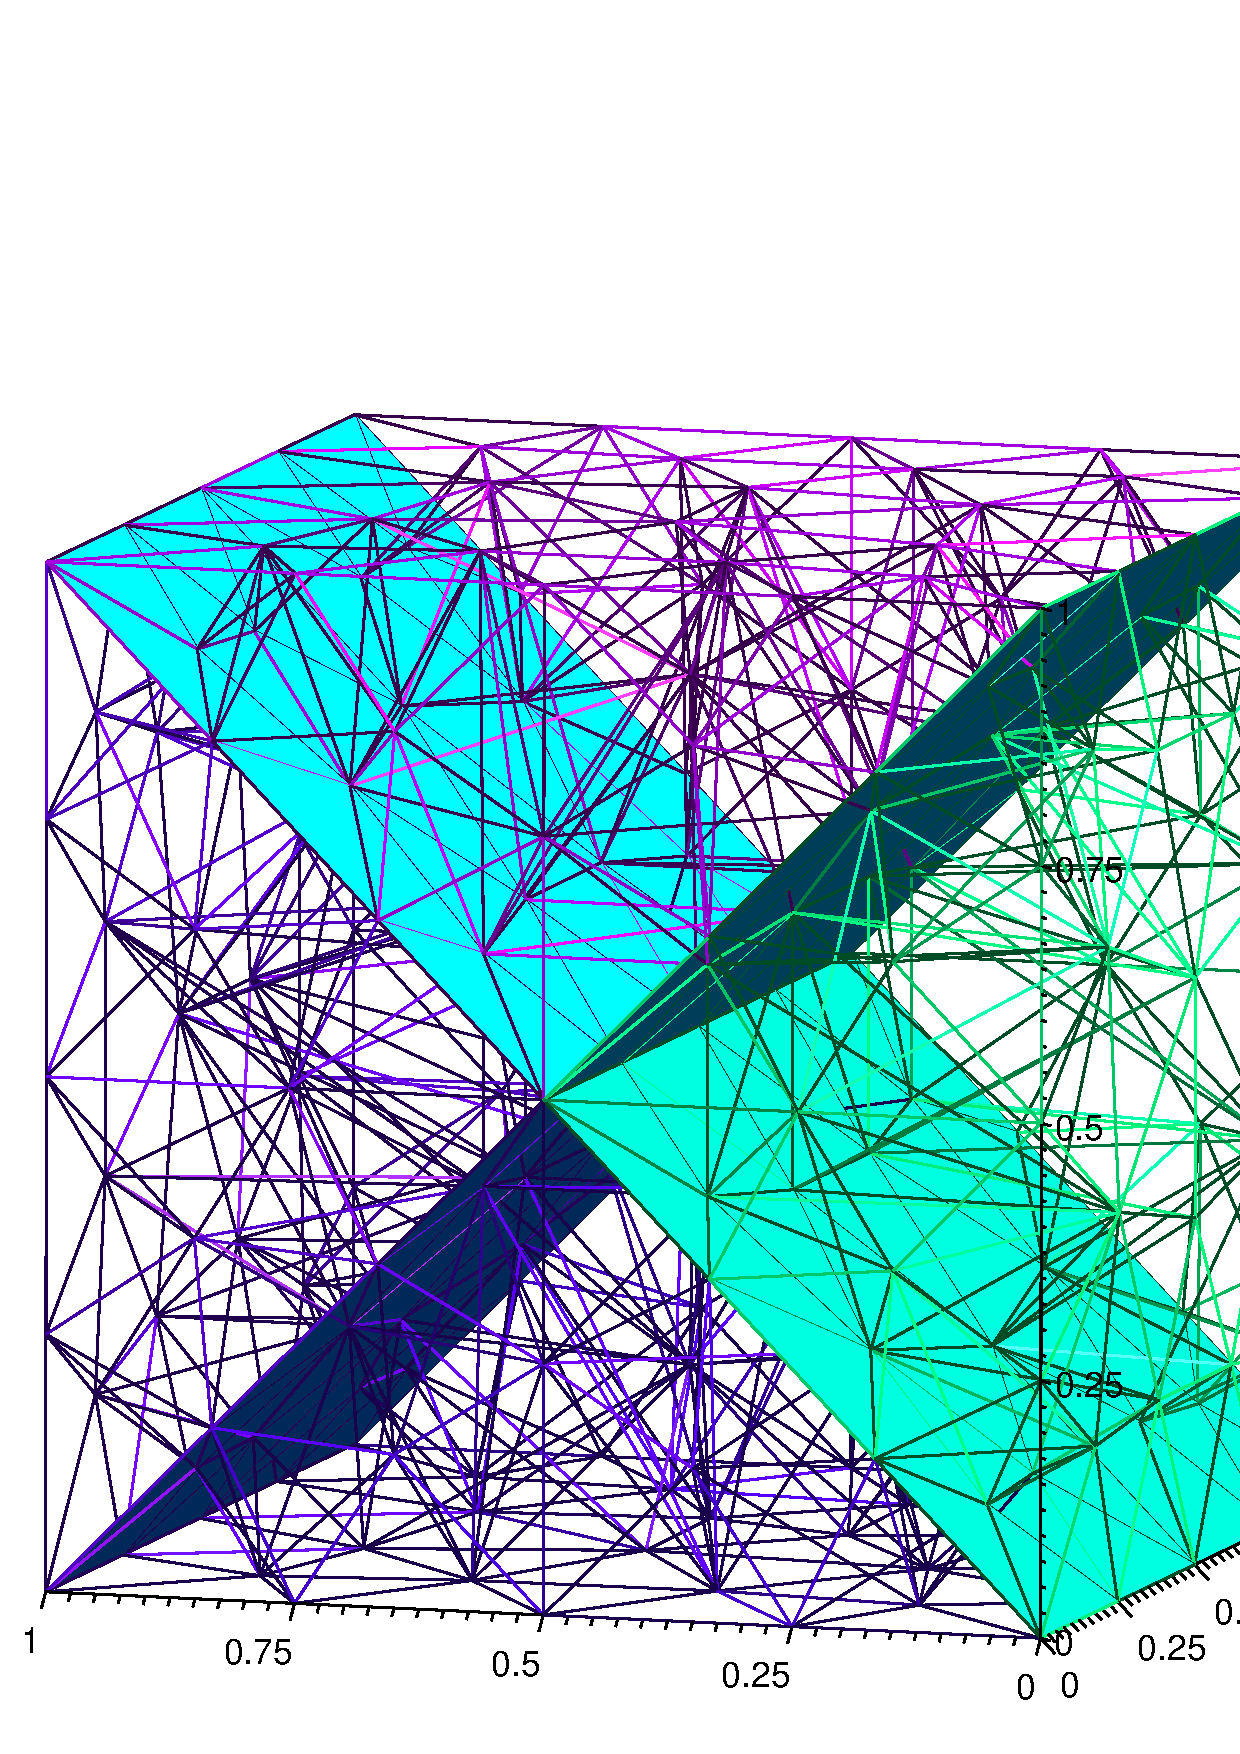
\includegraphics[width=13cm]{tests_graphics/01_mesh.pdf}
\caption{Test 01 -- mesh}
\label{fig:test1_mesh}
\end{figure}
%
%
\subsection*{Parameters}
\begin{itemize}
  \item \textbf{Cross section area:} 1D channel is set to 1.0~\unitss{}{2}{}.
  \item \textbf{Thickness:} 2D fractures are set to 1.0~\unitss{}{1}{}.
  \item \textbf{Conductivity:} The conductivity of materials:
    \begin{itemize}
      \item 1D channel is set to $K=10$~\unitss{}{1}{-1}.
      \item 2D fractures are set to $\mathbf{K}=\left(\begin{array}{cc} 1 & 0 \\ 0 & 1\end{array} \right)$~\unitss{}{1}{-1}.
      \item cube material is set to $\mathbf{K}=\left(\begin{array}{ccc} 0.1 & 0 & 0 \\ 0 & 0.1 & 0 \\ 0 & 0 & 0.1\end{array} \right)$~\unitss{}{1}{-1}.
    \end{itemize}
  \item There is no transport so there are not any other parameters.
\end{itemize}

\subsection*{Verification}
This test verifies solving steady Darcy flow by the mixed hybrid method. There are different dimensional connections 
which are 2D-3D connection between the cube and the flat fractures and 1D-2D connection between the 1D channel 
and the two flat fractures in their crossection. 

Following will not be commented in other examples and use of the functionalities will be considered apparent. No special test
programs are needed to test these as these are partially checked in the unit tests.

The input files \verb'flow_gmsh.con' and \verb'flow_vtk.con' give the same result, however the output is written in different 
formats. Also one can find an example of region set in \verb'flow_gmsh.con'.

Setting a Dirichlet boundary condition using piezometric head values is used in the input file \verb'flow_vtk_piezo.con'.
One can also notice using of the boundary set \verb'BOUNDARY' in this file. We use \emph{FieldFormula} to prescribe boundary
condition so this type of field and the function parser are also verified.

The remaining two files \verb'flow_old_vtk.con' and \verb'flow_vtk_fbc.con' use the obsolete way of defining boundary conditions.
The first one uses the old mesh without any named regions and the boundary condition file \verb'.fbc'. The second one combines
new mesh with named regions and the boudanry condition file created the old way. These tests ensure partially the backward 
compatibility of Flow123d with older input files.

%=====================================================
%                   TEST  2
%=====================================================

\section{Test 02 -- Steady flow in 2D and transport}
\label{sec:test02}
This test involves steady Darcy flow in 2D, connections of 1D-2D elements, Dirichlet boundary condition for flow and transport, 
transport of two substances with zero initial condition for concentration. There are actually two different cases computed in this test. 
Dual porosity and sorption features are present in the explicit transport. Dispersion is defined in the implicit transport.

The coefficient of diffusive transfer through a fracture (means between the fracture and the surrounding material) is set to 
zero so the substance cannot be diffused through the fracture's boundary.

  \begin{itemize} 
    \item \emph{problem type} -- sequential coupling 
    \item \emph{primary equation} -- steady mixed hybrid
    \item \emph{secondary equation} -- transport operator splitting (explicit), discontinuous Galerkin method (implicit)
  \end{itemize}

\subsection*{Geometry and boundary conditions}
The domain is two-dimensional slice through a part of a relief which involves several one-dimensional fractures.

Simple Dirichlet flow boundary condition is defined on left and right side where pressure heads are prescribed. 
There is no flow through the upper and lower boundary of the model. This all causes a flow along the x axis.

Dirichlet boundary condition for transport is prescribed on both sides as it is for flow boundary condition and 
the value of concentration is 1.0~\unitss{1}{-3}{} for both substances. Initial concentration of the substances 
is zero in the whole area. 
%
\begin{figure}[htb!]
\centering
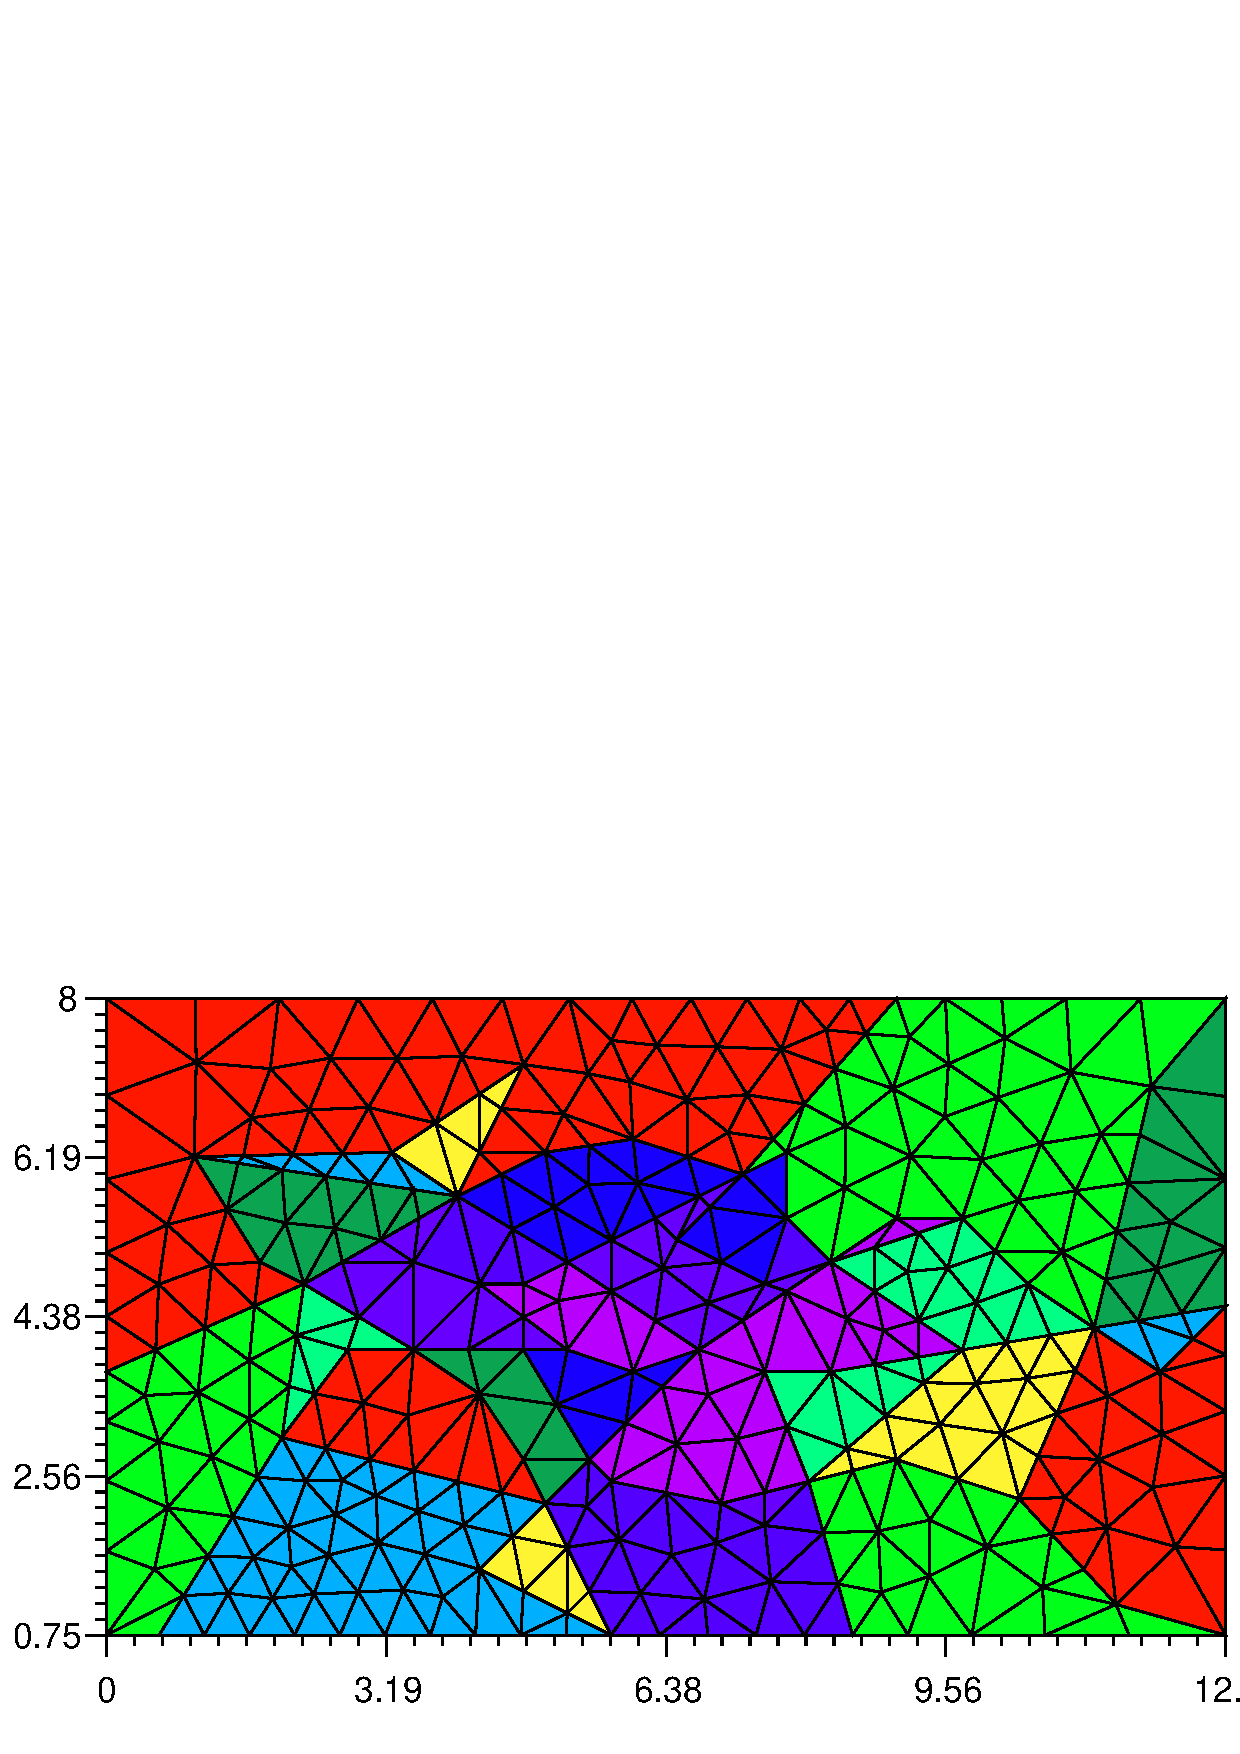
\includegraphics[width=15cm]{tests_graphics/02_mesh.pdf}
\caption{Test 02 -- mesh}
\label{fig:test2_mesh}
\end{figure}
%
%
\subsection*{Parameters}
The flow is steady and the transport is solved in time interval $(0,5.0)$~\unitss{}{}{1}. The output is written every 0.5~\unitss{}{}{1}. 
Time parameters for implicitly computed transport are the same only initial time step is set to 0.5~\unitss{}{}{1}.
\begin{itemize}
  \item \textbf{Cross section area:} 1D fractures are set to 1.0~\unitss{}{2}{}.
  \item \textbf{Thickness:} domain is set to 1.0~\unitss{}{1}{}.
  \item \textbf{Conductivity:} The conductivity of materials:
    \begin{itemize}
      \item fracture material is set to $K=10$~\unitss{}{1}{-1}.
      \item plane material is set to $\mathbf{K}=\left(\begin{array}{cc} 1 & 0 \\ 0 & 1\end{array} \right)$~\unitss{}{1}{-1}.
    \end{itemize}
  \item \textbf{Sorption:} The sorption parameters are for both materials equal:
    \begin{itemize}
      \item linear sorption isotherm parameter of the first substance is set to $k_l=0.02$.
      \item Freundlich sorption isotherm parameters of the second substance are set to $k_F=0.02$, $\alpha=0.5$  
    \end{itemize}
  \item \textbf{Dual porosity:} The dual porosity parameters are for both materials equal:
    \begin{itemize}
      \item mobile porosity coefficient is set to $0.25$
      \item immobile porosity coefficient is set to $0.25$
      \item nonequilibrium coefficient of both substances $0.01$
    \end{itemize}
  \item \textbf{Dispersion coefficients:} No dispersion is involved.
\end{itemize}

\subsection*{Verification}
This test verifies explicitly computed transport considering only convection with dual porosity and sorption and implicitly 
computed transport considering both convection and dispersion. Transport through 1D-2D element connections is computed in addition to the first test.



%=====================================================
%                   TEST  03
%=====================================================

\section{Test 03 -- Steady flow in 2D and transport}
\label{sec:test03}
This test differs from the previous one only by simpler structure of its geometry. It shows how the substace flows in the main fracture and divides in two other fractures. The substance spreads in the fractures much faster in comparision to transport in the plane.
\subsection*{Geometry and boundary conditions}
There is a plane with side 1.0 which is cutted by fractures. The main fracture divides in two other fractures.
\subsection*{Parameters}
The flow is steady and the transport is solved in time interval $(0,1.0)$. The output is written every 0.01. Initial time step for transport computed implicitly is set to 0.1 and the output is written every 0.1.

Other parameters are the same as in test 02.
\subsection*{Verification}
This test verifies the same features as the test 02 does but on a simpler geometry.



%=====================================================
%                   TEST  05
%=====================================================

\section{Test 05 -- Darcy flow boundary conditions}
\label{sec:test05}
There are three types of boundary conditions -- Dirichlet, Neumann and Robin that are tested. All three test have the same geometry and boundary conditions are derived from the same analytical solution.

We will prescribe analytical solution $u=xy$ of Laplace equation $-\Lapl{}u = 0$.
\begin{itemize} 
    \item \emph{problem type} -- sequential coupling 
    \item \emph{primary equation} -- steady mixed hybrid
  \end{itemize}

\subsection*{Geometry and boundary conditions}
The geometry is simple -- square plane in xy coordinates with corner points [0,0] and [1,1]. Each side has its own boundary regions called \verb0.bc_south0, \verb0.bc_east0, \verb0.bc_north0, \verb0.bc_west0.

\textbf{Dirichlet test.} All sides have pressure prescribed. These are south: $u_D=0$; east: $u_D=y$; north: $u_D=x$; west: $u_D=0$.

\textbf{Neumann test.} Two sides have pressure prescribed for the Dirichlet boundary condition: east: $u_D=y$; west: $u_D=0$. Two other sides have flux prescribed: south: $q_N=x$; north $q_N=-x$.

\textbf{Robin test.} Two sides have pressure prescribed  for the Dirichlet boundary condition: east: $u_D=y$; west: $u_D=0$.
For Robin boundary condition we get from the equation boundary pressure
\begin{equation} 
u_R=\frac{1+\sigma_R}{\sigma_R}x. 
\end{equation}
We choose $\sigma_R=0.5$ and then we get $u_R=-2x$ on the south side and $u_R=3x$ on the north side. 

\subsection*{Parameters}
\begin{itemize}
  \item \textbf{Conductivity:} on region \verb0plane0 is $1.0$~\unitss{}{1}{-1}.
  \item \textbf{Thickness:} on region \verb0plane0 is by default 1.0~\unitss{}{1}{}.
  \item There are no other regions, no transport so there are not any other parameters.
\end{itemize}

\subsection*{Verification}
This test verifies prescribing different types of boundary conditions.


%=====================================================
%                   TEST  06
%=====================================================

\section{Test 06 -- Coupling between dimensions in Darcy flow}
\label{sec:test06}
There are two tests -- \verb'flow_32d.con' for compatible coupling between 3D-2D and \verb'flow_21d.con' for compatible coupling between 2D-1D.

\begin{itemize} 
    \item \emph{problem type} -- sequential coupling 
    \item \emph{primary equation} -- steady mixed hybrid
  \end{itemize}

We will discuss both the geometry and parameters at once.

%
\begin{figure}[h!]
\centering
\includegraphics[width=0.6\textwidth]{tests_graphics/06_result_32d.pdf}
\caption{Test 06 -- solution. For verification see the blue plate where the constant 
         piezometric head -3~\unitss{}{1}{} is.}
\label{fig:test6_solution_32d}
\end{figure}
%
\textbf{3D-2D.}
There is a cube with vertices [0,0,0] [-1,-1,-1] which couples with a 2D crack in the bottom (i.e. $z=-1$~\unitss{}{1}{}).
We consider solution of the piezometric head in the cube $p_3(x,y,z) = z$. We will use it to 
prescribe Dirichlet boundary condition on the non-coupling parts of the cube.
There are no sources of a flow in the cube. 
We can write the outflow through the bottom of the cube in following term 
$q_{32} = \mathbf{q_3} \cdot \mathbf{n} = (- K_3 \nabla p_3(x,y,-1))\cdot \mathbf{n}$,
where $\mathbf{n}=(0,0,-1)$.
To obtain Laplace equation with zero right hand side on the 2D crack, we prescribe a new source 
term (\ref{eqn:test06_f2}) that eliminates the inflow coming from the cube.         
\begin{eqnarray}
    F_2 &=& \delta_2  f_2 + q_{32} = 0   \nonumber\\
    f_2(x,y) &=& -\frac{q_{32}}{\delta_2}   \label{eqn:test06_f2}.
\end{eqnarray}
When $\delta_2 = 10$~\unitss{}{1}{}, $K_3 = 2$~\unitss{}{1}{-1} are choosed then the source term is equal $f_2 = -0.2$~\unitss{}{}{-1}.
Homogenous Neumann condition is prescribed on the boundary of the fraction (zero outflow and inflow).

From the flow coupling equation we can get the piezometric head (\ref{eqn:test06_p2}) on the crack which we can verify.
\begin{eqnarray} 
     \sigma_{32}  ( p_3(x,y,-1) - p_2(x,y) ) &=& q_{32} \nonumber\\
     p_2(x,y) &=& -\frac{q_{32}}{\sigma_{32}} + p_3(x,y,-1) \label{eqn:test06_p2}.
\end{eqnarray}   
When $\sigma_{32} = 1$~\unitss{}{}{-1} is set then the piezometric head in the crack is constant and equal $p_2(x,y) = -3$~\unitss{}{1}{}
as we can see in figure \ref{fig:test6_solution_32d}.

%
\begin{figure}[h!]
\centering
\includegraphics[width=0.6\textwidth]{tests_graphics/06_result_21d.pdf}
\caption{Test 06 -- solution. For verification see the blue channel on the left side of the plane 
         where the constant piezometric head -2.5~\unitss{}{1}{} is.}
\label{fig:test6_solution_21d}
\end{figure}
%
\textbf{2D-1D.}
The other tests geometry consists of a 2D crack in $xy$ plane with vertices [0,0] [1,1] and a 1D channel coupling with the crack on the left side ($x=0$). 
Everything is then analogical to the first test.
We consider solution of the pressure in the crack $p_2(x,y) = x$. We will use it to prescribe Dirichlet boundary condition on the non-coupling parts of the crack.
There are no sources of a flow in the crack. 
We can write the outflow through the left side of the crack in the following term $q_{21} = \mathbf{q_2} \cdot \mathbf{n} = (- \delta_2 K_2 \nabla p_2(0,y))\cdot \mathbf{n}$,
where $\mathbf{n}=(-1,0)$.
To obtain Laplace equation with zero right hand side on the channel, we prescribe a new source term (\ref{eqn:test06_f1}) that eliminates the inflow coming from the crack.         
\begin{eqnarray}
    F_1 &=& \delta_1  f_1 + q_{21} = 0   \nonumber\\
    f_1(x,y) &=& -\frac{q_{21}}{\delta_1}   \label{eqn:test06_f1}.
\end{eqnarray}
When $\delta_1 = 20$~\unitss{}{2}{}, $\delta_2 = 10$~\unitss{}{1}{} and $K_2 = 5$~\unitss{}{1}{-1} are choosed then the source term is equal $f_2 = -2.5$~\unitss{}{}{-1}.
Homogenous Neumann condition is prescribed on the boundary of the fraction (zero outflow and inflow).

From the flow coupling equation we can get the pressure (\ref{eqn:test06_p1}) on the plane which we can verify.
\begin{eqnarray} 
     \delta_2 \sigma_{21} ( p_2(0,y) - p_2(y) ) &=& q_{21} \nonumber\\
     p_1(y) &=& -\frac{q_{21}}{\delta_2 \sigma_{21}} + p_2(0,y) \label{eqn:test06_p1}.
\end{eqnarray}   
When $\sigma_{21} = 1$~\unitss{}{}{-1} is set then the pressure in the crack is constant and equal $p_1(y) = -2.5$~\unitss{}{1}{}
as we can see in the figure \ref{fig:test6_solution_21d}.

% \subsection*{Parameters}
% Parameters where discussed above.

\subsection*{Verification}
This test verifies correct communication between dimensions 3D-2D and 2D-1D in compatible coupling.
We can also observe the results in the \verb'water_balance' file. We should see that all the inflow 
to the cube should be fully compensated by the negative source. Homogenous Neumann boundary condition 
is prescribed on the crack so there should be no outflow or inflow through the boundary of the crack.
The situation in the second test is similar. The inflow to the crack should be fully compensated by 
the negative source in the channel which should have no other inflow or outflow.


%=====================================================
%                   TEST  8
%=====================================================

\section{Test 08 -- Steady Darcy flow with source}
\label{sec:test08}
This test is aimed at verifying steady Darcy flow with source which is prescribed by function formula. 
We will solve Laplace equation $-\Lapl{}u = f$ where source $f$ is prescribed by function $f = 2(1-y^2) + 2(1-x^2)$.
We can easily prove that (\ref{eqn:test8}) is the analytic solution by replacing it in the Laplace equation.
\begin{equation}
u = (1-x^2)(1-y^2) \label{eqn:test8}
\end{equation}

  \begin{itemize} 
    \item \emph{problem type} -- sequential coupling 
    \item \emph{primary equation} -- steady mixed hybrid
  \end{itemize}

\subsection*{Geometry and boundary conditions}
The domain is a square with opposite vertices $[-1,-1]$ and $[1,1]$. Zero dirichlet boundary condition is prescribed 
on all boundaries -- along the circumference of the square.
 
\subsection*{Parameters}
\begin{itemize}
  \item \textbf{Conductivity:} The conductivity of plane material is $1.0$~\unitss{}{1}{-1}.
  \item There are no other materials, no transport so there are not any other parameters.
\end{itemize}
%
\begin{figure}[h!]
\centering
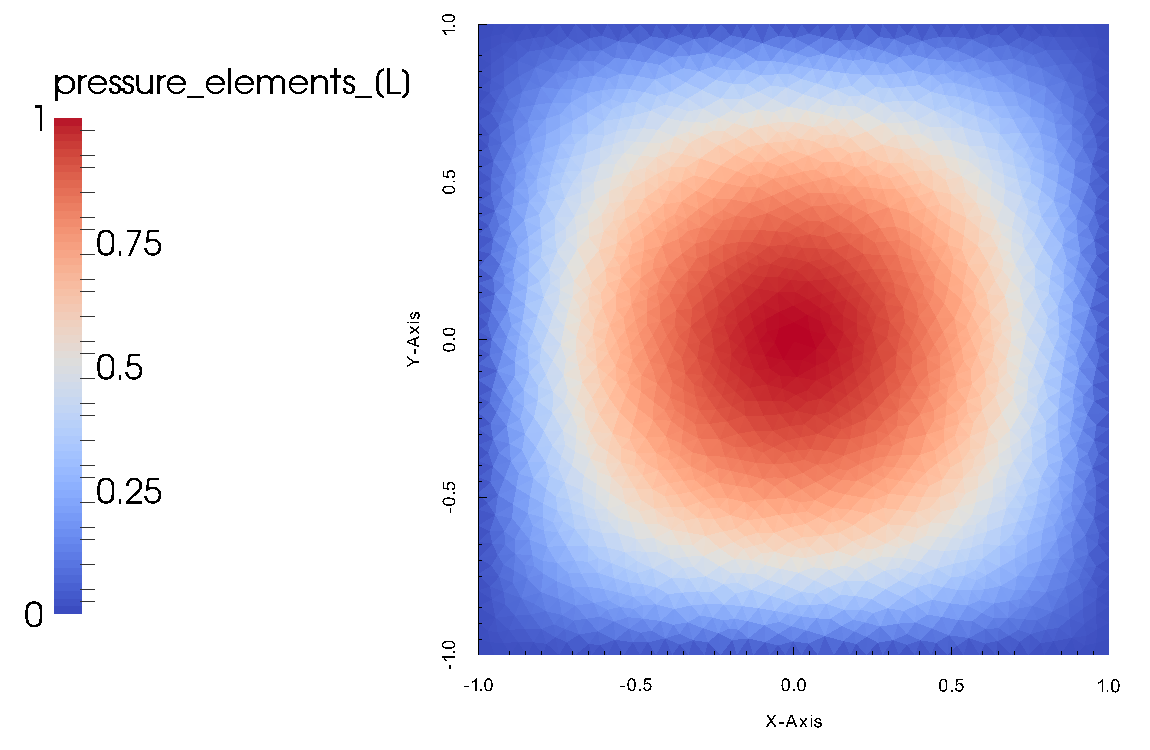
\includegraphics[width=0.8\textwidth]{tests_graphics/08_solution.pdf}
\caption{Test 08 -- solution. Distribution of the pressure matches the analytical solution (\ref{eqn:test8}).}
\label{fig:test8_solution}
\end{figure}
%
\subsection*{Verification}
The solution (pressure) is a paraboloid with a top in $[0,0,1]$ as we can see in the figure \ref{fig:test8_solution}. 
One can verify the equality in Paraview using the prepared state file.


%=====================================================
%                   TEST  10
%=====================================================

\section{Test 10 -- Unsteady flow in 2D}
\label{sec:test10}
Unsteady flow in 2D domain is simulated in this test and is computed by both mixed hybrid and 
lumped mixed hybrid method. No transport is involved. 

\begin{itemize} 
    \item \emph{problem type} -- sequential coupling
    \item \emph{primary equation} -- unsteady mixed hybrid, unsteady lumped mixed hybrid
  \end{itemize}

\subsection*{Geometry and boundary conditions}
The domain is a square with oposite vertices $[0,0]$ and $[1,1]$. Different Dirichlet boundary condition for 
pressure is prescribed on two opposite sides -- 0.0~\unitss{}{1}{} on the left and 100.0~\unitss{}{1}{} on the right.

\subsection*{Parameters}
The flow is solved in time interval $(0,0.5)$ with step 0.01~\unitss{}{}{1}. The output is written every 0.1~\unitss{}{}{1}.
\begin{itemize}
  \item \textbf{Conductivity:} The conductivity of plane material is $0.02$~\unitss{}{1}{-1}.
  \item Initial pressure is set to zero everywhere.
  \item There are no other materials, no transport so there are not any other parameters.
\end{itemize}

\subsection*{Verification}
This test verifies two different numerical methods -- the problem is computed by both mixed hybrid and lumped mixed hybrid method.

%=====================================================
%                   TEST  11
%=====================================================

\section{Test 11 -- Radioactive decay chain with more branches}
8 isotopes are members of considered decay chain with three branches. Transport boundary conditions does not matter 
because zero presure gradient is considered. Final concentrations of all isotopes except C decrease to zero after 20 
time steps, whereas C concentration grows to 0.36.
\[
 E\xrightarrow{}D\xrightarrow{}F\xrightarrow{}B
 \quad
 \begin{matrix}
    0.2B\xrightarrow{}A & A\xrightarrow{}G \\
    0.6B\xrightarrow{}H & H\xrightarrow{}G \\
    0.2B\xrightarrow{}G &\\
 \end{matrix}
 \quad
 G\xrightarrow{}C 
\]

\begin{itemize} 
    \item \emph{problem type} -- sequential coupling
    \item \emph{primary equation} -- steady mixed hybrid
    \item \emph{secondary equation} -- transport operator splitting
    \item \emph{reactions} -- linear reactions
  \end{itemize}

\subsection*{Geometry}
The domain is a prism which base is a right-angled triangle with its ordinates 3.0~\unitss{}{1}{}. 
There are only three tetrahedron elements in the mesh.

\subsection*{Parameters}
The flow is steady and the transport is solved in time interval $(0,10.0)$~\unitss{}{}{1}. The output is written every 0.5~\unitss{}{}{1}.

Half-lives are equal to 0.5 for all isotopes. Initial concentrations are summarized in the table below:
  \begin{center}
    \begin{tabular}[c]{|l|c|c|c|c|c|c|c|c|}
      \hline
      isotop & A & B  & C & D & E & F & G & H \\[4pt]
      initial concentration & 0.01 & 0.02 & 0.03 & 0.04 & 0.05 & 0.06 & 0.07 & 0.08 \\[4pt]
      \hline
    \end{tabular}
  \end{center}


\subsection*{Verification}


%=====================================================
%                   TEST  12
%=====================================================

\section{Test 12 -- Radioactive decay}
There are actually two tests of the radioactive decay. The first one considers first order reaction of two isotopes 
determined by kinetic constant and the other one describes radioactive decay chain of three isotopes.

\begin{itemize} 
    \item \emph{problem type} -- sequential coupling
    \item \emph{primary equation} -- steady mixed hybrid
    \item \emph{secondary equation} -- transport operator splitting
    \item \emph{reactions} -- linear reactions
  \end{itemize}

\subsection*{Geometry and boundary conditions}
The domain is a prism which base is a right-angled triangle with its ordinates 3.0 units long. There are then only three tetrahedron elements in the mesh.

There are two Dirichlet boundary conditions for flow prescribed.

\begin{itemize}
  \item \textbf{Conductivity:} The conductivity of the prism material is $0.01$~\unitss{}{1}{-1}. 
  \item There is no other parameter for flow or transport.
\end{itemize}



\subsection{First order reaction determined by kinetic constant}
The only linear reaction between D and F substances.
\[
D\xrightarrow{k}F
\]

\subsection*{Parameters}
The flow is steady and the transport is solved in time interval $(0,10.0)$. The output is written every 0.5~\unitss{}{}{1}.  
\begin{itemize}
  \item \textbf{Substances:} 6 substances to be transported -- A, B, C, D, E, F
  \item \textbf{Kinetic constant:} $k = 0.277258872$
\end{itemize}

\subsection*{Verification}

\subsection{Radioactive decay chain}
The considered radioctive decay chain is:
\[
 D\xrightarrow{t_{1/2,D}}F\xrightarrow{t_{1/2,F}}B
\]
\subsection*{Parameters}
Time parameters are the same as they are above.
\begin{itemize}
  \item \textbf{Substances:} 6 substances to be transported -- A, B, C, D, E, F
  \item \textbf{Decay half-lives:} $t_{1/2,D} = t_{1/2,F} = 2.5$
\end{itemize}

\subsection*{Verification}

% Both following tests are realized without combination with transport (zero pressure gradient).
% verification of:
% - first order reaction A->B determined by kinetic constant,
% -- 6 chemical species (A, B, .., F) are transported but just 2 of them take a part in considered first order kinetic reaction wich looks as follows
% --- D->F, appropriate kinetic constant is k = 0.277258872.
% --- Initail conditions look as follows, A(0) = 0.01, B(0) = 0.02, C(0) = 0.03, D(0) = 0.04, E(0) = 0.05, F(0) = 0.06.
% --- Transport boundary conditions does not matter because zero presure gradient is considered.
% --- Final concentrations of all isotopes except A, B, C, E do not change. Concentrations of D decreases to 0.003. Concentration of F increase to 0.85 in 20 time steps.

% - narrow radioctive decay chain without branches, A -> B -> C,
% -- 6 isotopes (A, B, .., F) are transported but just 3 of them are members of considered decay chain which looks as folows
% --- D->F->B
% --- Initail conditions look as follows, A(0) = 0.01, B(0) = 0.02, C(0) = 0.03, D(0) = 0.04, E(0) = 0.05, F(0) = 0.06.
% --- Transport boundary conditions does not matter because zero presure gradient is considered.
% --- Final concentrations of all isotopes except A, C, E do not change. Concentrations of D and B decrease to 0.004 and 0.012 respectively. Concentration of B increase to 0.1 in 20 time steps.

%=====================================================
%                   TEST  13
%=====================================================

\section{Test 13 -- Solute mixing on the edge}
This test realizes mixing of substances on the edges of planes and also does quantitative test on a trivial 
transport problem. The problem is computed with both explicit and implicit transport.

\begin{itemize} 
    \item \emph{problem type} -- sequential coupling 
    \item \emph{primary equation} -- steady mixed hybrid
    \item \emph{secondary equation} -- transport operator splitting (explicit), discontinuous Galerkin method (implicit)
  \end{itemize}

\subsection*{Geometry and boundary conditions}
The domain is a fork where the main branch with the incoming solute is 5~\unitss{}{1}{} long and lies in 
the $xy$ plane. Then it is divided into two other branches $5\sqrt{2}$~\unitss{}{1}{} long, one with 
positive and the another with negative $z$ coordinate. There are different conductivities in each branch.

Dirichlet boundary conditions for flow and transport are prescribed at the beginning of the main 
plane ($x=0$~\unitss{}{1}{}) and at the ends of the secondary branches ($x=10$~\unitss{}{1}{}).

flow: $h_D=-x-z+10.0$ which gives 10.0~\unitss{}{1}{} at point [0,0,0] and $\pm5$~\unitss{}{1}{} at points [10,0,$\mp5$]\\
transport: concentration is 1.0 at point [0,0,0] and 0.0 at points [10,0,$\mp5$]

Initial concentration of the substances is zero in the whole area. 
%
\subsection*{Parameters}
The flow is steady and the transport is solved in time interval $(0,100.0)$~\unitss{}{}{1}. 
The output is written every 5~\unitss{}{}{1}. 
Time parameters for implicitly computed transport are the same only initial time step and output time is set to 5.0~\unitss{}{}{1}.
\begin{itemize}
  \item \textbf{Thickness:} all planes are set to 1.0~\unitss{}{1}{}.
  \item \textbf{Conductivity:} The conductivity of materials (isotropic planes):
    \begin{itemize}
      \item main branch (material num. 17): $K=1$~\unitss{}{1}{-1}.
      \item branch (positive $z$, material num. 18): $K=0.1$~\unitss{}{1}{-1}.
      \item branch (negative $z$, material num. 19): $K=0.1$~\unitss{}{1}{-1}.
    \end{itemize}
  \item \textbf{Dispersion coefficients:} Default parameters are set in implicit transport, so no dispersion is present. 
        For more details see \hyperlink{IT::TransportDG-BulkData}{TransportDG\_BulkData} in the input reference.
\end{itemize}
%
\begin{figure}[!h]
    \centering
    \begin{subfigure}[b]{0.45\textwidth}
        \centering
        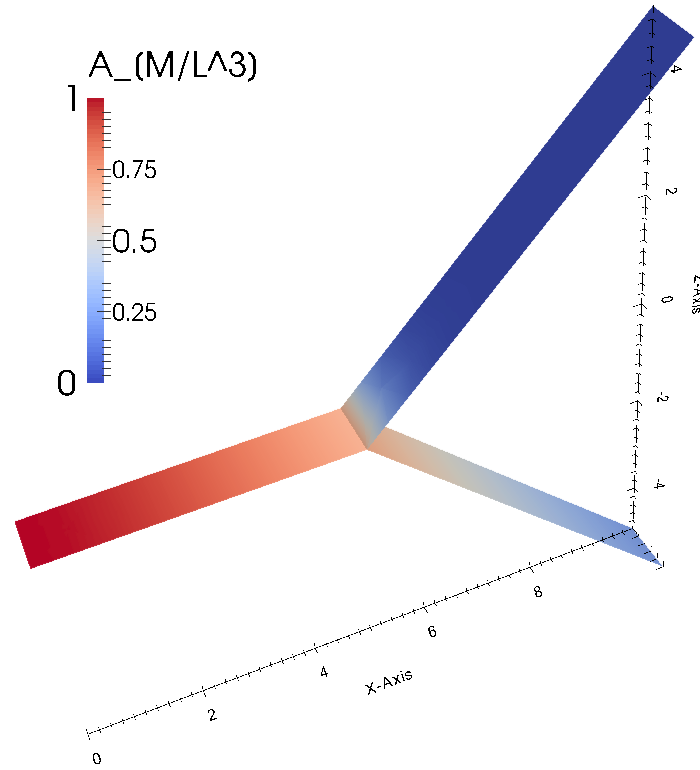
\includegraphics[width=\textwidth]{tests_graphics/13_solution_t2.pdf}
        \caption{Solution at time 10~\unitss{}{}{1}.}
        \label{fig:test13_a}
    \end{subfigure}
    ~
    \begin{subfigure}[b]{0.45\textwidth}
        \centering
        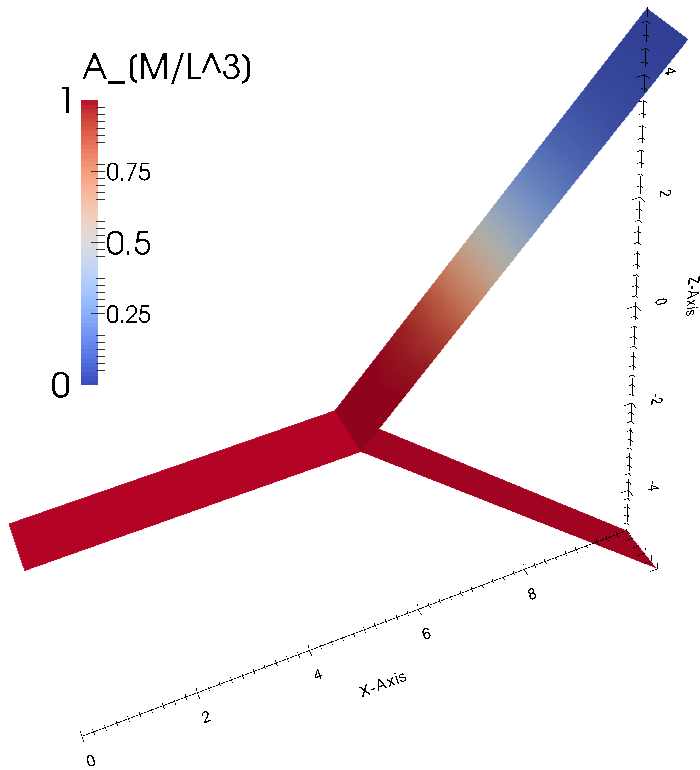
\includegraphics[width=\textwidth]{tests_graphics/13_solution_t10.pdf}
        \caption{Solution at time 10~\unitss{}{}{1}.}
        \label{fig:test13_b}
    \end{subfigure}
    \caption{Test 13 -- mesh}
  \label{fig:test13}
\end{figure}
%
\subsection*{Verification}
This test verifies qualitatively both the problem of flow and transport. We can see the influence of smaller conductivity 
in upper branch in the figure \ref{fig:test13}. The concentration of the substance spreads slower in the upper branch than 
in the lower one.

%=====================================================
%                   TEST  14
%=====================================================

\section{Test 14 -- Variable transport boundary condition}
We consider a time variable boundary condition for transport in this test. Steady flow with constant velocity is caused by a pressure 
gradient from one side of a 2D strip to the another. Dirichlet boundary condition for transport evolving in time is prescribed on the 
right side using set of older \verb'.tbc' files. 

\begin{itemize} 
    \item \emph{problem type} -- sequential coupling, 
    \item \emph{primary equation} -- steady mixed hybrid
    \item \emph{secondary equation} -- transport operator splitting (explicit), discontinuous Galerkin method (implicit)
  \end{itemize}

\subsection*{Geometry and boundary conditions}

Dirichlet boundary condition for pressure is prescribed $h_D = x$ all around the plane and causes constant flow from right to left 
(pressure prescribed on the upper and lower sides are equal along x axis so causes no flow). Transport boundary condition has 
the same prescribtion as for the pressure, only the values evolves in time.

Initial concentration is zero on the whole plane. Two pulses of nonzero concentration are applied on the boundary. The changes 
of the boundary condition at specified times are shown in the following table:
%
\begin{center}
  \begin{tabular}{|l|c|c|c|c|c|}
    \hline
    time \units{}{}{1} & $0$ & $1$ & $3$ & $6$ & $7$\\
    concentration & $0$ & $20$ & $0$ & $40$ & $0$\\
    \hline
  \end{tabular}
\end{center}

\begin{figure}[htb!]
\centering
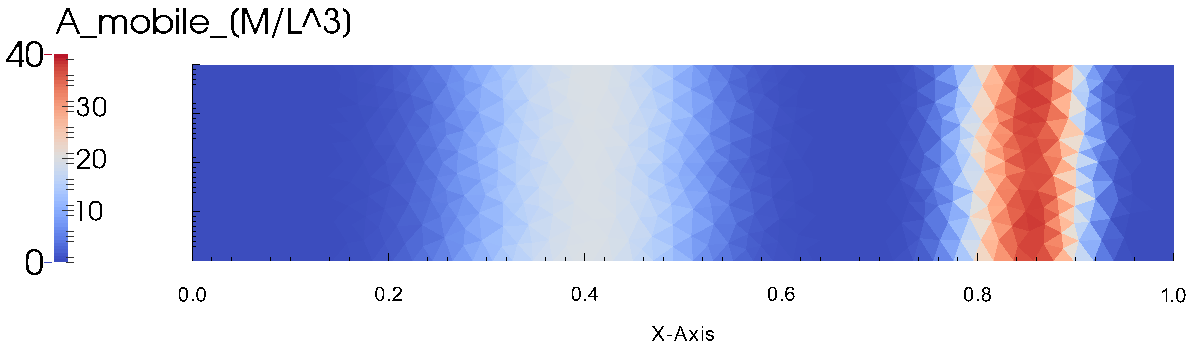
\includegraphics[width=15cm]{tests_graphics/14_solution.pdf}
\caption{Test 14 -- solution at time 8.0~\unitss{}{}{1}.}
\label{fig:test14_mesh}
\end{figure}
%
%
\subsection*{Parameters}
The flow is steady and the transport is solved in time interval $(0,10.0)$~\unitss{}{}{1}. The output is written every 
1.0~\unitss{}{}{1}. Time parameters for implicitly computed transport are the same only initial time step is set to 1.0~\unitss{}{}{1}.
%
\begin{itemize}
  \item \textbf{Thickness:} all planes are set to 1.0~\unitss{}{1}{}.
  \item \textbf{Conductivity:} The conductivity of material (isotropic plane): $K=0.1$~\unitss{}{1}{-1}.
  \item \textbf{Dispersion coefficients:} Default parameters are set in implicit transport, so no dispersion is present. 
        For more details see \hyperlink{IT::TransportDG-BulkData}{TransportDG\_BulkData} in the input reference.
\end{itemize}
%

\subsection*{Verification}
This test verifies that the transport boundary condition can evolve in time. We use old \verb'.tbc' for description 
of the transport boundary condition but all other possibilities work also.


%=====================================================
%                   TEST  15
%=====================================================

\section{Test 15 -- Unsteady flow with transport}
Transport of a single pulse of concentration moving along a 2D strip is solved. This test involves unsteady flow computed by lumped hybrid method, transport is solved both with explicit and implicit (involves dispersion) scheme.
 
\begin{itemize} 
    \item \emph{problem type} -- sequential coupling, 
    \item \emph{primary equation} -- unsteady lumped mixed hybrid
    \item \emph{secondary equation} -- transport operator splitting (explicit), discontinuous Galerkin method (implicit)
  \end{itemize}

\subsection*{Geometry and boundary conditions}
The domain is a 2D strip with dimensions $1.0$x$16.0$. Zero Dirichlet boundary for flow is prescribed at $x=0$, zero Neumann boundary is elsewhere. 

Dirichlet transport boundary condition is set on the left side to 10.0 only at the beginning. Then is this boundary condition zero.

\subsection*{Parameters}
Initial pressure is zero everywhere. 
The source is prescribed with function $f=-x$ along the strip.
%
\begin{itemize}
  \item \textbf{Thickness:} all planes are set to 1.0~$L$.
  \item \textbf{Conductivity:} The conductivity of material (isotropic plane): $K=1.0$.
  \item \textbf{Source formula:} $f = -x$
  \item \textbf{Diffusivity coefficients:} are used in implicit transport wth dispersion. 
	Default parameters are set ($d_m=1e-6$, others are zero, see manual or parameters in test02 in ~\ref{sec:test02}).
\end{itemize}
%
\begin{figure}[htb!]
\centering
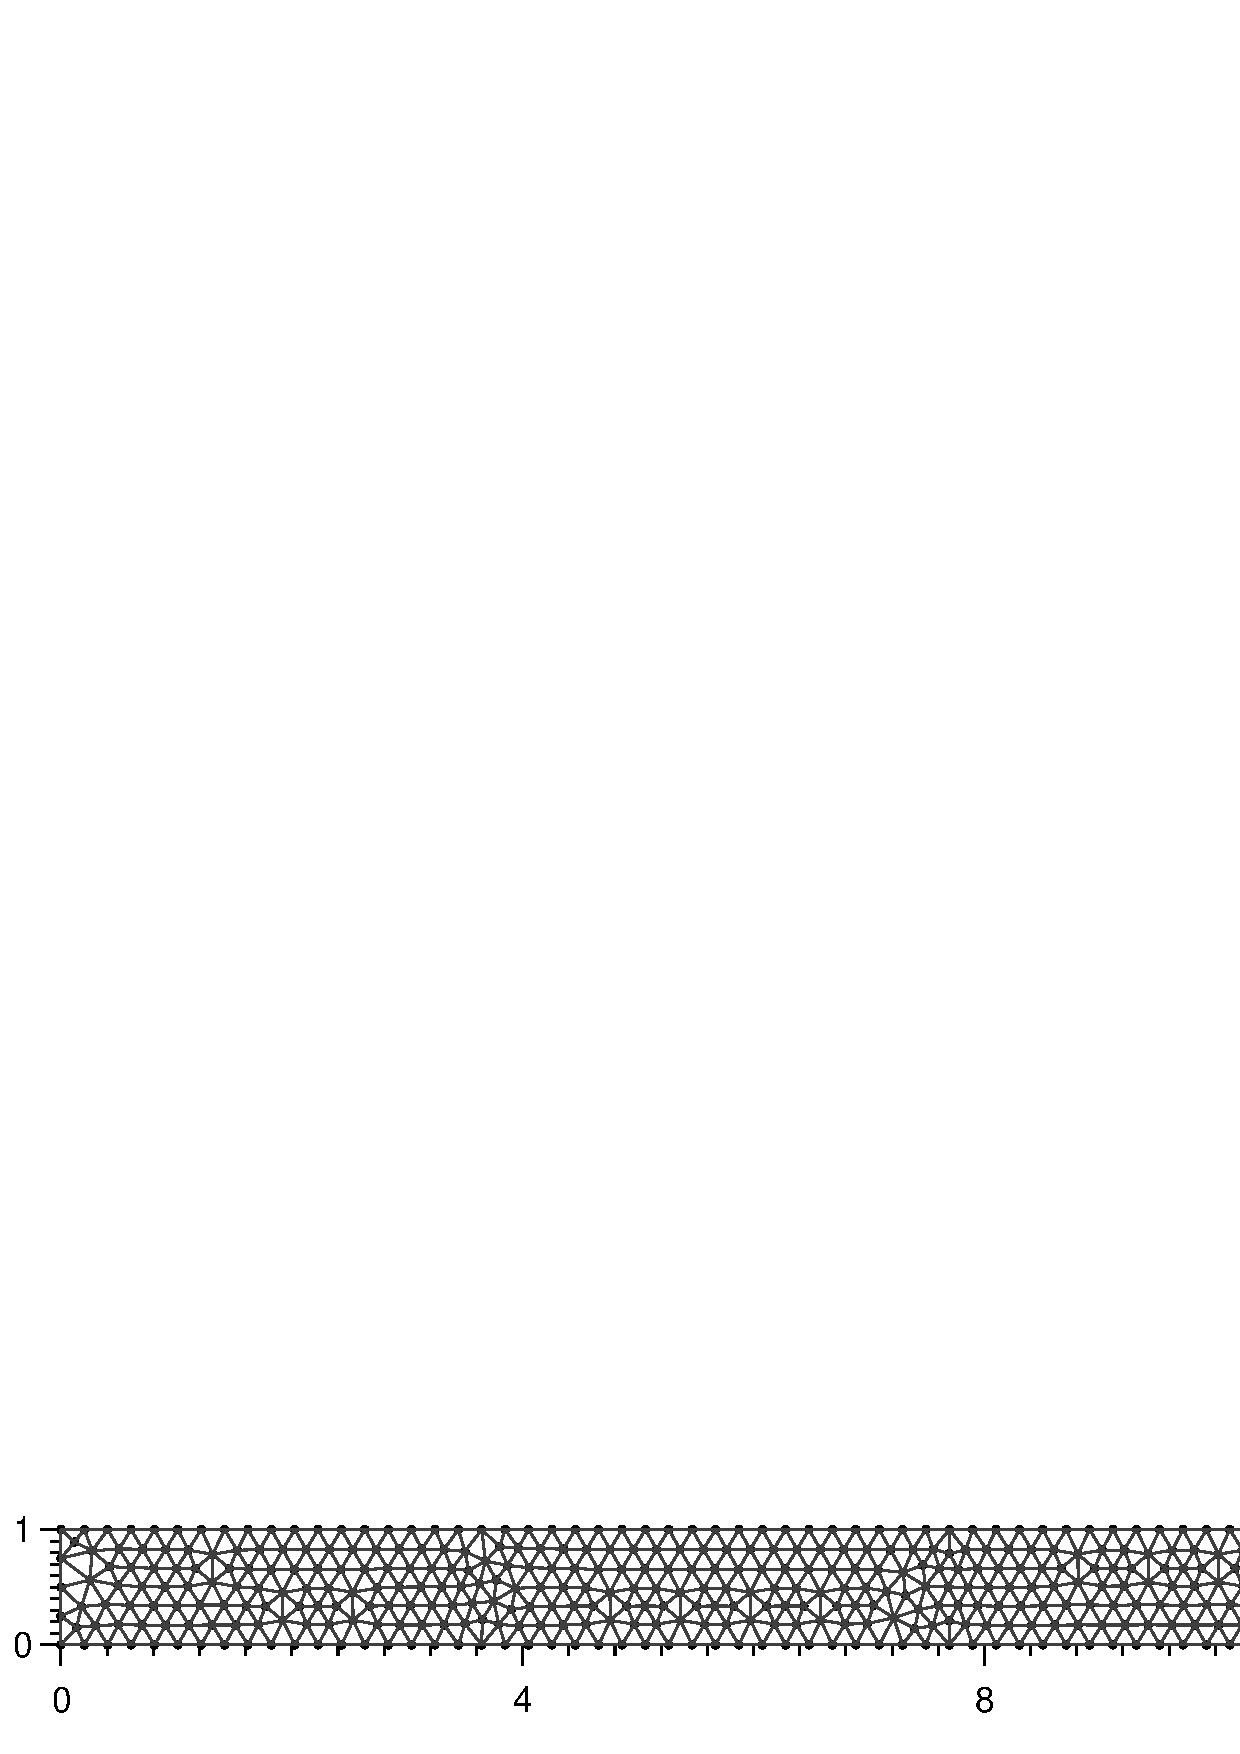
\includegraphics[width=15cm]{tests_graphics/15_mesh.pdf}
\caption{Test 15 -- mesh}
\label{fig:test15_mesh}
\end{figure}
%
%
\subsection*{Verification}
The test is similar to the test 10 but here in addition the computation of a transport in an unsteady flow field is verified.


%=====================================================
%                   TEST  16
%=====================================================

\section{Test 16 -- Substance concentration source in transport}
This test include a source of concentration of a substance. The domain is a 2D strip in vertical direction. There is a steady flow with constant velocity in the vertical direction. Two sources are situated on two elements at the top of the strip and the substance is transported down along the strip. The concentration values of the sources are defined in the \verb0tso0 input file.

\begin{itemize} 
    \item \emph{problem type} -- sequential coupling, 
    \item \emph{primary equation} -- steady mixed hybrid
    \item \emph{secondary equation} -- transport operator splitting
  \end{itemize}

\subsection*{Geometry}


\subsection*{Parameters}

\subsection*{Verification}



%=====================================================
%                   TEST  17
%=====================================================

\section{Test 17 -- Radioactive decay -- Pade approximation}
This test solves radioactive decay chain of five isotopes using Pade approximation.
The considered radioctive decay chain is:
\[
 A\xrightarrow{t_{1/2,A}}B\xrightarrow{t_{1/2,B}}C\xrightarrow{t_{1/2,C}}D\xrightarrow{t_{1/2,D}}E
\]

\begin{itemize} 
    \item \emph{problem type} -- sequential coupling, 
    \item \emph{primary equation} -- steady mixed hybrid
    \item \emph{secondary equation} -- transport operator splitting
    \item \emph{reactions} -- Pade approximation
  \end{itemize}

\subsection*{Geometry}
The geometry and material and transport parameters are the same as in test 12.


\subsection*{Parameters}
\begin{itemize}
  \item \textbf{Substances:} 5 substances to be transported -- A, B, C, D, E
  \item Polynomial degree of the nominator and the denominator of Pade approximation is~3.
  \item \textbf{Decay half-lives:} 
    \begin{tabular}[c]{|c|c|c|c|}
      \hline
      $t_{1/2,A}$ & $t_{1/2,B}$  & $t_{1/2,C}$ & $t_{1/2,D}$\\[4pt]
      $1.3863$ & $2.3105$ & $1.5403$ & $1.1552$\\[4pt]
      \hline
    \end{tabular}
\end{itemize}

\subsection*{Verification}


%=====================================================
%                   TEST  18
%=====================================================

\section{Test 18 -- Diffusion through fractures}
This test is aimed at transport caused just by diffusion. 

There is a triangular domain with zero pressure everywhere so no flow is present. Triangular element 
with high concentration of a substance lies in the middle of the domain and its sides neighbour with fractures.
The coeffients of molecular diffusion and diffusive transfer through fractures are the parameters of 
the implicit transport and are set in the configuration file.

\subsection*{Geometry}

\subsection*{Parameters}

\subsection*{Verification}


%=====================================================
%                   TEST  18
%=====================================================

\section{Test 19 -- Boundary condition interpolation}

The input file \verb'large_cube_solution.msh' for interpolation was computed from \verb'flow_large_gmsh.con'.

To view comparision of the large mesh and small mesh with interpolated bc
compute \verb'flow_large_vtk.con' and then add results when opening Paraview with state file.

\begin{itemize} 
    \item \emph{problem type} -- sequential coupling, 
    \item \emph{primary equation} -- steady mixed hybrid
    \item \emph{secondary equation} -- transport operator splitting
  \end{itemize}

\subsection*{Geometry}


\subsection*{Parameters}

\subsection*{Verification}
verification of interpolation of boundary condition for piezohead


\section{Analytical solution for transport equation}
Lokking for $u(t,x)$ satisfying
\[
   \prtl_t u - d \prtl^2_x u + b \prtl_x u =0
\]
on domain $[0,\infty)\times [0,L]$. Using separation of variables $u(t,x) = T(t)X(x)$, have equations
\[
    T' - kd T =0,\qquad X''-\alpha X' - k X=0
\]
with $\alpha=\frac{b}{d}$ The first equation has solution
\[
   T(t) = c e^{kt}.
\]
Since, we are looking only for stable solutions, we assume $k\ge0$. The second equation, has solution
\[
   X(x)=c_1e^{\lambda_1 x}+c_2e^{\lambda_2 x},\quad \lambda_{1,2} = \frac{\alpha \pm \sqrt{\alpha^2 + 4k}}{2}.
\]

We consider Dirichlet boundary conditions $u(t,0)=1$ and $u(t,L)=0$. For these, we get particular steady solution
\[
  u_p(x) = \frac{e^{\alpha x} - e^{\alpha L}}{1-e^{\alpha L}}.
\]

Next, we shall solve problem with homogeneous boundary conditions. We consider only discrete part of the spectrum, that is 
$\alpha^2 +4k = -\alpha^2\omega^2$. From homogeneous boundary conditions, we obtain solutions

\[
   u_n(t,x) = e^{k_n t} e^{\frac{\alpha}{2} x} \sin\big( \frac{\pi n}{L} x \big),\quad k_n = -\frac{\alpha^2}{4}\big(\frac{4\pi^2n^2}{L^2\alpha^2} +1 \big)
\]

Then the whole solution is
\[
  u(t,x) = u_p(t,x) + \sum_{n=1}^{\infty} a_n u_n(t,x)
\]
where $a_n$ are Fourier coefficients (just sinus part) of the function $u_0(x) - u_p(x)$.














% ===================  PREPARING  ==================
% \section{Test 20 -- Dirichlet boundary condition}
% \label{sec:test20}
% This test involves steady Darcy flow in 3D determined by Dirichlet boundary condition. The analytic solution is prescribed $u = xyz$. We can see from the formula that there are no sources $-\Lapl{}u = 0$ (zero right hand side) and we can easily define Dirichlet boundary conditions on the sides of the cube just by evaluating the solution there.
% 
% \subsection*{Geometry}
% The domain is a cube with its side 1.0~$L$ long.
% Dirichlet boundary conditions are summarized in the following table. Physical domains corresponds with the numbers in \verb0geo0 file, the row \emph{plane} contains equations of the planes (sides of the cube). The row \emph{Dirichlet} contains solution on the planes. The row \emph{boundary} segment contains numbers of segments defined in \verb0con0 file.
% 
% \begin{center}
%   \begin{tabular}{|l|c|c|c|c|c|c|}
%       \hline
%       boundary segment & 1 & 2 & 3 & 4 & 5 & 6 \\ 
%       physical domain & 27 & 28 & 29 & 30 & 31 & 32 \\ 
%       plane & $z-1=0$  & $x-1=0$ & $z=0$ & $x=0$ & $y-1=0$& $y=0$\\
%       Dirichlet [$u_D$] & $xy$ & $yz$ & $0$ & $0$ & $xz$ & $0$\\
%       \hline
%   \end{tabular}
% \end{center}
% 
% \subsection*{Parameters}
% \begin{itemize}
%   \item \textbf{Conductivity:} cube material is set to $\mathbf{K}=\left(\begin{array}{ccc} 1.0 & 0 & 0 \\ 0 & 1.0 & 0 \\ 0 & 0 & 1.0\end{array} \right)$.
%   \item There is no transport so there are not any other parameters.
% \end{itemize}
% 
% \subsection*{Verification}
% This test verifies prescribing Dirichlet boundary condition.
% 
% 
% \section{Test 21 -- Neumann boundary condition}
% \label{sec:test21}
% This test uses the same geometry and parameters as in the test 20 (viz~\ref{sec:test20}) but there are prescribed both Dirichlet and Neumann boundary conditions. 
% 
% The table of the boundary conditions is below. The row \emph{Dirichlet} contains contains solution on the planes and the row \emph{Neumann} contains flow through the planes.
% 
% \begin{center}
%   \begin{tabular}{|l|c|c|c|c|c|c|}
%       \hline
%       boundary segment & 1 & 2 & 3 & 4 & 5 & 6 \\ 
%       physical domain & 27 & 28 & 29 & 30 & 31 & 32 \\ 
%       plane & $z-1=0$  & $x-1=0$ & $z=0$ & $x=0$ & $y-1=0$& $y=0$\\
%       Dirichlet [$u_D$] 
% 	  &   -   & $yz$ & $0$ & $0$ &   -   & $0$\\
%       Neumann [$-\nabla{}u\cdot{}\mathbf{n}$] 
% 	  & $-xy$ &   -  &  -  &  -  & $-xz$ & - \\
%       \hline
%   \end{tabular}
% \end{center}
% 
% \subsection*{Verification}
% This test verifies prescribing Neumann boundary condition.
% 
% \section{Test 22 -- Newton boundary condition}
% \label{sec:test21}
% This test uses the same geometry and parameters as in the test 20 (viz~\ref{sec:test20}) but there is prescribed Newton boundary condition $-\nabla{}u\cdot{}\mathbf{n} = \sigma(u-u_T)$.
% 
% The table of the boundary conditions where parameters $\sigma$ and $u_T$ are written is below. The values of parameters were chosen to satisfy condition $-\nabla{}u\cdot{}\mathbf{n} = -(yz,xz,xy)\cdot\mathbf{n} = \sigma(u-u_T)$
% 
% \begin{center}
%   \begin{tabular}{|l|c|c|c|c|c|c|}
%       \hline
%       boundary segment & 1 & 2 & 3 & 4 & 5 & 6 \\ 
%       physical domain & 27 & 28 & 29 & 30 & 31 & 32 \\ 
%       plane & $z-1=0$  & $x-1=0$ & $z=0$ & $x=0$ & $y-1=0$& $y=0$\\
%       $-\nabla{}u\cdot{}\mathbf{n}$ & $-xy$ & $-yz$ & $xy$ & $yz$ & $-xz$ &\\
%       $\sigma$ & $xy$ & $yz$ & $0$ & $0$ & $xz$ & $0$\\
%       $u_T$ & $u_T=xy$ & $u=yz$ & $u=0$ & $u=0$ & $u=xz$ & $u=0$\\
%       \hline
%   \end{tabular}
% \end{center}
% 
% \subsection*{Verification}
% This test verifies prescribing Newton boundary condition.

% 
%  \chapter{Comparision of versions (WORK IN PROGRESS)}
%  \label{chapter:version_comparision}
%  \input{version_comparision}

\chapter{Main Input File Reference}
\label{chapter:input-tree-reference}
% support macros

% generated file
\begin{RecordType}
	{IT::Root}
	{Root}
	{}% implements
	{}% reducible to key
	{{{Root record of JSON input for Flow123d.}% 
}}
		\RecKey
			{Root::flow123d-version}
			{flow123d{\_}version}
			{{String}}{}
			{ \it{Obligatory}}
			{{{Version of Flow123d for which the input file was created.
Flow123d only warn about version incompatibility.
However, external tools may use this information to provide conversion of the input file to the structure required by another version of Flow123d.}% 
}}
		\RecKey
			{Root::problem}
			{problem}
			{{abstract: }\TypeLink{IT::Coupling-Base}{Coupling{\_}Base}}{}
			{ \it{Obligatory}}
			{{{Simulation problem to be solved.}% 
}}
		\RecKey
			{Root::pause-after-run}
			{pause{\_}after{\_}run}
			{{Bool}}{}
			{ \ValueDefault{false}}
			{{{If true, the program will wait for key press before it terminates.}% 
}}
\end{RecordType}
\begin{AbstractType}
	{IT::Coupling-Base}
	{Coupling{\_}Base}
	{}
	{{{The root record of description of particular the problem to solve.}% 
}}
		\Descendant{\TypeLink{IT::Coupling-Sequential}{Coupling{\_}Sequential}}% 
\end{AbstractType}
\begin{RecordType}
	{IT::Coupling-Sequential}
	{Coupling{\_}Sequential}
	{\TypeLink{IT::Coupling-Base}{Coupling{\_}Base}}% implements
	{}% reducible to key
	{{{Record with data for a general sequential coupling.}% 
}}
		\RecKey
			{Coupling-Sequential::time}
			{time}
			{{record: }\TypeLink{IT::TimeGovernor}{TimeGovernor}}{}
			{ \ValueDefault{{\{}{\}}}}
			{{{Time governor setting.}% 
}}
		\RecKey
			{Coupling-Sequential::description}
			{description}
			{{String}}{}
			{ \it{Optional}}
			{{{Short description of the solved problem.}\\{
Is displayed in the main log, and possibly in other text output files.}% 
}}
		\RecKey
			{Coupling-Sequential::mesh}
			{mesh}
			{{record: }\TypeLink{IT::Mesh}{Mesh}}{}
			{ \it{Obligatory}}
			{{{Computational mesh common to all equations.}% 
}}
		\RecKey
			{Coupling-Sequential::flow-equation}
			{flow{\_}equation}
			{{abstract: }\TypeLink{IT::DarcyFlow}{DarcyFlow}}{}
			{ \it{Obligatory}}
			{{{Flow equation, provides the velocity field as a result.}% 
}}
		\RecKey
			{Coupling-Sequential::solute-equation}
			{solute{\_}equation}
			{{abstract: }\TypeLink{IT::AdvectionProcess}{AdvectionProcess}}{}
			{ \it{Optional}}
			{{{Transport of soluted substances, depends on the velocity field from a Flow equation.}% 
}}
		\RecKey
			{Coupling-Sequential::heat-equation}
			{heat{\_}equation}
			{{abstract: }\TypeLink{IT::AdvectionProcess}{AdvectionProcess}}{}
			{ \it{Optional}}
			{{{Heat transfer, depends on the velocity field from a Flow equation.}% 
}}
\end{RecordType}
\begin{RecordType}
	{IT::TimeGovernor}
	{TimeGovernor}
	{}% implements
	{\TypeLink{TimeGovernor::max-dt}{max{\_}dt}}% reducible to key
	{{{Time axis settings of the simulation.}\\{
The settings is specific to a particular equation.}\\{
TimeGovernor allows to:}\\{
 - define start time and end time of simulation}\\{
 - define lower and upper limits of time steps}\\{
 - direct fixed time marks of whole simulation}\\{
 - set global time unit of equation (see 'common{\_}time{\_}unit' key)}\\{
Limits of time steps are defined by keys 'min{\_}dt', 'max{\_}dt', 'init{\_}dt' and 'dt{\_}limits'. Key 'init{\_}dt' has the highest priority and allows set fix size of time steps.
Pair of keys 'min{\_}dt' and 'max{\_}dt' define interval of time steps.
Both previous cases ('init{\_}dt' or pair 'min{\_}dt' and 'max{\_}dt') set global limits of whole simulation.
In contrasts, 'dt{\_}limits' allow set time-dependent function of min{\_}dt/max{\_}dt.
Used time steps of simulation can be printed to YAML output file (see 'write{\_}used{\_}timesteps'.}\\{
Fixed time marks define exact values of time steps.
They are defined in:}\\{
 - start time and end time of simulation}\\{
 - output times printed to output mesh file}\\{
 - times defined in 'dt{\_}limits' table (optional, see 'add{\_}dt{\_}limits{\_}time{\_}marks' key)}% 
}}
		\RecKey
			{TimeGovernor::start-time}
			{start{\_}time}
			{{tuple: }\TypeLink{IT::TimeValue}{TimeValue}}{}
			{ \ValueDefault{0.0}}
			{{{Start time of the simulation.}% 
}}
		\RecKey
			{TimeGovernor::end-time}
			{end{\_}time}
			{{tuple: }\TypeLink{IT::TimeValue}{TimeValue}}{}
			{ \ValueDefault{5e+17}}
			{{{End time of the simulation.}\\{
The default value is higher than the age of the Universe (given in seconds).}% 
}}
		\RecKey
			{TimeGovernor::init-dt}
			{init{\_}dt}
			{{tuple: }\TypeLink{IT::TimeValue-2}{TimeValue}}{}
			{ \ValueDefault{0.0}}
			{{{Initial guess for the time step.}\\{
It applies to equations that use an adaptive time stepping.
If set to 0.0, the time step is determined in fully autonomous way, assuming the equation supports it.}% 
}}
		\RecKey
			{TimeGovernor::min-dt}
			{min{\_}dt}
			{{tuple: }\TypeLink{IT::TimeValue-2}{TimeValue}}{}
			{implicit value: "{Machine precision.}"}
			{{{Soft lower limit for the time step.}\\{
Equation using an adaptive time stepping cannot suggest smaller time step.
The actual time step can only decrease below the limit in order to match the prescribed input or output times.}% 
}}
		\RecKey
			{TimeGovernor::max-dt}
			{max{\_}dt}
			{{tuple: }\TypeLink{IT::TimeValue-2}{TimeValue}}{}
			{implicit value: "{Whole time of the simulation if specified, infinity else.}"}
			{{{Hard upper limit for the time step.}\\{
The actual time step can only increase above the limit in order to match the prescribed input or output times.}% 
}}
		\RecKey
			{TimeGovernor::dt-limits}
			{dt{\_}limits}
			{{array [0, UINT] of }{tuple: }\TypeLink{IT::DtLimits}{DtLimits}}{}
			{ \it{Optional}}
			{{{Allow to set a time dependent changes in }\begin{ttfamily}min{\_}dt\end{ttfamily}{ and }\begin{ttfamily}max{\_}dt\end{ttfamily}{ limits.
This list is processed at individual times overwriting previous values of }\begin{ttfamily}min{\_}dt\end{ttfamily}{/}\begin{ttfamily}max{\_}dt\end{ttfamily}{. Limits equal to 0 are ignored and replaced with }\begin{ttfamily}min{\_}dt\end{ttfamily}{/}\begin{ttfamily}max{\_}dt\end{ttfamily}{ values.}% 
}}
		\RecKey
			{TimeGovernor::add-dt-limits-time-marks}
			{add{\_}dt{\_}limits{\_}time{\_}marks}
			{{Bool}}{}
			{ \ValueDefault{false}}
			{{{Add all times defined in }\begin{ttfamily}dt{\_}limits\end{ttfamily}{ table to the list of fixed TimeMarks.}% 
}}
		\RecKey
			{TimeGovernor::write-used-timesteps}
			{write{\_}used{\_}timesteps}
			{{Filename}}{}
			{ \it{Optional}}
			{{{Write used time steps to the given file in YAML format corresponding with the format of }\begin{ttfamily}dt{\_}limits\end{ttfamily}{.}% 
}}
		\RecKey
			{TimeGovernor::common-time-unit}
			{common{\_}time{\_}unit}
			{{record: }\TypeLink{IT::Unit}{Unit}}{}
			{ \ValueDefault{"s"}}
			{{{Common time unit of the equation.}\\{
This unit will be used for all time inputs and outputs within the equation.
Individually, the common time unit can be overwritten for every declared time.}\\{
Time units are used in the following cases:}\\{
1) Time units of time value keys in: TimeGovernor, FieldDescriptors.}\\{
   The common time unit can be overwritten for every declared time.}\\{
2) Time units in: }\\{
   a) input fields: FieldFE and FieldTimeFunction}\\{
   b) time steps definition of OutputTimeSet}\\{
   Common time unit can be overwritten by one unit value for every whole mesh data file or time function.}\\{
3) Time units in output files: observation times, balance times, frame times of VTK and GMSH}\\{
   Common time unit cannot be overwritten in these cases.}% 
}}
\end{RecordType}
\begin{TupleType}
	{IT::TimeValue}
	{TimeValue}
	{}% implements
	{\TypeLink{TimeValue::time}{time}}% reducible to key
	{{{A time with optional unit specification.}% 
}}
		\RecKey
			{TimeValue::time}
			{time}
			{{Double (-inf, +inf)}}{}
			{ \it{Obligatory}}
			{{{The time value.}% 
}}
		\RecKey
			{TimeValue::unit}
			{unit}
			{{record: }\TypeLink{IT::Unit}{Unit}}{}
			{implicit value: "{Common time unit of the equation's Time Governor.
See the key 'common{\_}time{\_}unit'.}"}
			{{{{Predefined units include: }\begin{ttfamily}s\end{ttfamily}{ seconds, }\begin{ttfamily}min\end{ttfamily}{ minutes, }\begin{ttfamily}h\end{ttfamily}{ hours, }\begin{ttfamily}d\end{ttfamily}{ days, }\begin{ttfamily}y\end{ttfamily}{ years.}\\{
The default time unit is set from the equation's time governor, see the key }\begin{ttfamily}common{\_}time{\_}unit\end{ttfamily}{in the equation's time record.}
% 
}{{User can benefit from the Unit Convertor funcionality and create different time units.}\\{
Year length example considering leap years (Gregorian calendar): }\begin{ttfamily}year; year = 365.2425*d\end{ttfamily}{.}\\{
Miliseconds example : }\begin{ttfamily}milisec; milisec = 0.001*s\end{ttfamily}{.}% 
}}}
\end{TupleType}
\begin{RecordType}
	{IT::Unit}
	{Unit}
	{}% implements
	{\TypeLink{Unit::unit-formula}{unit{\_}formula}}% reducible to key
	{{{{Specify the unit of an input value.
Evaluation of the unit formula results into a coeficient and a unit in terms of powers of base SI units.
The unit must match theexpected SI unit of the value, while the value provided on the input is multiplied by the coefficient before further processing.
The unit formula have a form:}\\
\begin{ttfamily}{\textless}UnitExpr{\textgreater};{\textless}Variable{\textgreater}={\textless}Number{\textgreater}*{\textless}UnitExpr{\textgreater};...,\end{ttfamily}\\{
where }\begin{ttfamily}{\textless}Variable{\textgreater}\end{ttfamily}{ is a variable name and }\begin{ttfamily}{\textless}UnitExpr{\textgreater}\end{ttfamily}{ is a units expression which consists of products and divisions of terms.}
% 
}{{A term has a form: }\begin{ttfamily}{\textless}Base{\textgreater}{\^{}}{\textless}N{\textgreater}\end{ttfamily}{, where }\begin{ttfamily}{\textless}N{\textgreater}\end{ttfamily}{ is an integer exponent and }\begin{ttfamily}{\textless}Base{\textgreater}\end{ttfamily}{ is either a base SI unit, a derived unit, or a variable defined in the same unit formula.
Example, unit for the pressure head:}
% 
}{{}\begin{ttfamily}MPa/rho/g{\_}; rho = 990*kg*m{\^{}}-3; g{\_} = 9.8*m*s{\^{}}-2\end{ttfamily}% 
}}}
		\RecKey
			{Unit::unit-formula}
			{unit{\_}formula}
			{{String}}{}
			{ \it{Obligatory}}
			{{{Definition of unit.}% 
}}
\end{RecordType}
\begin{TupleType}
	{IT::TimeValue-2}
	{TimeValue}
	{}% implements
	{\TypeLink{TimeValue-2::time}{time}}% reducible to key
	{{{A time with optional unit specification.}% 
}}
		\RecKey
			{TimeValue-2::time}
			{time}
			{{Double [0, +inf)}}{}
			{ \it{Obligatory}}
			{{{The time value.}% 
}}
		\RecKey
			{TimeValue-2::unit}
			{unit}
			{{record: }\TypeLink{IT::Unit}{Unit}}{}
			{implicit value: "{Common time unit of the equation's Time Governor.
See the key 'common{\_}time{\_}unit'.}"}
			{{{{Predefined units include: }\begin{ttfamily}s\end{ttfamily}{ seconds, }\begin{ttfamily}min\end{ttfamily}{ minutes, }\begin{ttfamily}h\end{ttfamily}{ hours, }\begin{ttfamily}d\end{ttfamily}{ days, }\begin{ttfamily}y\end{ttfamily}{ years.}\\{
The default time unit is set from the equation's time governor, see the key }\begin{ttfamily}common{\_}time{\_}unit\end{ttfamily}{in the equation's time record.}
% 
}{{User can benefit from the Unit Convertor funcionality and create different time units.}\\{
Year length example considering leap years (Gregorian calendar): }\begin{ttfamily}year; year = 365.2425*d\end{ttfamily}{.}\\{
Miliseconds example : }\begin{ttfamily}milisec; milisec = 0.001*s\end{ttfamily}{.}% 
}}}
\end{TupleType}
\begin{TupleType}
	{IT::DtLimits}
	{DtLimits}
	{}% implements
	{\TypeLink{DtLimits::time}{time}}% reducible to key
	{{{Time dependent changes in min{\_}dt and max{\_}dt limits.}% 
}}
		\RecKey
			{DtLimits::time}
			{time}
			{{tuple: }\TypeLink{IT::TimeValue}{TimeValue}}{}
			{ \it{Obligatory}}
			{{{The start time of dt step set.}% 
}}
		\RecKey
			{DtLimits::min-dt}
			{min{\_}dt}
			{{tuple: }\TypeLink{IT::TimeValue}{TimeValue}}{}
			{implicit value: "{'min{\_}dt' value of TimeGovernor.}"}
			{{{Soft lower limit for the time step.}% 
}}
		\RecKey
			{DtLimits::max-dt}
			{max{\_}dt}
			{{tuple: }\TypeLink{IT::TimeValue}{TimeValue}}{}
			{implicit value: "{'max{\_}dt' value of TimeGovernor.}"}
			{{{Whole time of the simulation if specified, infinity else.}% 
}}
\end{TupleType}
\begin{RecordType}
	{IT::Mesh}
	{Mesh}
	{}% implements
	{\TypeLink{Mesh::mesh-file}{mesh{\_}file}}% reducible to key
	{{{Record with mesh related data.}% 
}}
		\RecKey
			{Mesh::mesh-file}
			{mesh{\_}file}
			{{Filename}}{}
			{ \it{Obligatory}}
			{{{Input file with mesh description.}% 
}}
		\RecKey
			{Mesh::regions}
			{regions}
			{{array [0, UINT] of }{abstract: }\TypeLink{IT::Region}{Region}}{}
			{ \it{Optional}}
			{{{{List of additional region and region set definitions not contained in the mesh.
There are three region sets implicitly defined:}
% 
}
\begin{itemize}
\item {ALL (all regions of the mesh)}
\item {.BOUNDARY (all boundary regions)}
\item {BULK (all bulk regions)}
\end{itemize}
}}
		\RecKey
			{Mesh::partitioning}
			{partitioning}
			{{record: }\TypeLink{IT::Partition}{Partition}}{}
			{ \ValueDefault{"any{\_}neighboring"}}
			{{{Parameters of mesh partitioning algorithms.}% 
}}
		\RecKey
			{Mesh::print-regions}
			{print{\_}regions}
			{{Bool}}{}
			{ \ValueDefault{true}}
			{{{If true, print table of all used regions.}% 
}}
		\RecKey
			{Mesh::intersection-search}
			{intersection{\_}search}
			{{selection: }\TypeLink{IT::Types-of-search-algorithm-for-finding-intersection-candidates-}{Types of search algorithm for finding intersection candidates.}}{}
			{ \ValueDefault{"BIHsearch"}}
			{{{Search algorithm for element intersections.}% 
}}
		\RecKey
			{Mesh::global-snap-radius}
			{global{\_}snap{\_}radius}
			{{Double [0, +inf)}}{}
			{ \ValueDefault{0.001}}
			{{{Maximal snapping distance from the mesh in various search operations.
In particular, it is used to find the closest mesh element of an observe point; and in FieldFormula to find closest surface element in plan view (Z projection).}% 
}}
		\RecKey
			{Mesh::raw-ngh-output}
			{raw{\_}ngh{\_}output}
			{{Filename}}{}
			{ \it{Optional}}
			{{{Output file with neighboring data from mesh.}% 
}}
		\RecKey
			{Mesh::optimize-mesh}
			{optimize{\_}mesh}
			{{Bool}}{}
			{ \ValueDefault{true}}
			{{{If true, permute nodes and elements in order to increase cache locality.
This will speed up the calculations.
GMSH output preserves original ordering but is slower.
All variants of VTK output use the permuted.}% 
}}
\end{RecordType}
\begin{AbstractType}
	{IT::Region}
	{Region}
	{}
	{{{Abstract record for Region.}% 
}}
		\Descendant{\TypeLink{IT::From-Id}{From{\_}Id}}% 
		\Descendant{\TypeLink{IT::From-Label}{From{\_}Label}}% 
		\Descendant{\TypeLink{IT::From-Elements}{From{\_}Elements}}% 
		\Descendant{\TypeLink{IT::Union}{Union}}% 
		\Descendant{\TypeLink{IT::Difference}{Difference}}% 
		\Descendant{\TypeLink{IT::Intersection}{Intersection}}% 
\end{AbstractType}
\begin{RecordType}
	{IT::From-Id}
	{From{\_}Id}
	{\TypeLink{IT::Region}{Region}}% implements
	{}% reducible to key
	{{{Elementary region declared by its id.}\\{
It allows to create a new region with given id and name, or to rename an existing region of given id.}% 
}}
		\RecKey
			{From-Id::name}
			{name}
			{{String}}{}
			{ \it{Obligatory}}
			{{{Name (label) of the region.
It has to be unique per single mesh.}% 
}}
		\RecKey
			{From-Id::id}
			{id}
			{{Integer [0, INT]}}{}
			{ \it{Obligatory}}
			{{{Id of the region to which you assign the name.}% 
}}
		\RecKey
			{From-Id::dim}
			{dim}
			{{Integer [0, INT]}}{}
			{ \it{Optional}}
			{{{Dimension of the region to which you assign the name.}\\{
The value is taken into account only if a new region is created.}% 
}}
\end{RecordType}
\begin{RecordType}
	{IT::From-Label}
	{From{\_}Label}
	{\TypeLink{IT::Region}{Region}}% implements
	{}% reducible to key
	{{{Elementary region declared by its name (label).}\\{
It gives a new name to an elementary region with the original name (in the mesh file) given by the }\begin{ttfamily}mesh{\_}label.\end{ttfamily}% 
}}
		\RecKey
			{From-Label::name}
			{name}
			{{String}}{}
			{ \it{Obligatory}}
			{{{New name (label) of the region.
It has to be unique per single mesh.}% 
}}
		\RecKey
			{From-Label::mesh-label}
			{mesh{\_}label}
			{{String}}{}
			{ \it{Obligatory}}
			{{{The original region name in the input file, e.g. a physical volume name in the GMSH format.}% 
}}
		\RecKey
			{From-Label::allow-empty}
			{allow{\_}empty}
			{{Bool}}{}
			{ \ValueDefault{false}}
			{{{If true it allows to the region set to be empty (no elements).}% 
}}
\end{RecordType}
\begin{RecordType}
	{IT::From-Elements}
	{From{\_}Elements}
	{\TypeLink{IT::Region}{Region}}% implements
	{}% reducible to key
	{{{Elementary region declared by a list of elements.}\\{
The new region is assigned to the list of elements specified by the key }\begin{ttfamily}element{\_}list\end{ttfamily}{.}% 
}}
		\RecKey
			{From-Elements::name}
			{name}
			{{String}}{}
			{ \it{Obligatory}}
			{{{Name (label) of the region.
It has to be unique per single mesh.}% 
}}
		\RecKey
			{From-Elements::id}
			{id}
			{{Integer [0, INT]}}{}
			{ \it{Optional}}
			{{{Id of the region.
If unset, a unique id will be generated automatically.}% 
}}
		\RecKey
			{From-Elements::element-list}
			{element{\_}list}
			{{array [1, UINT] of }{Integer [0, INT]}}{}
			{ \it{Obligatory}}
			{{{List of ids of elements.}% 
}}
\end{RecordType}
\begin{RecordType}
	{IT::Union}
	{Union}
	{\TypeLink{IT::Region}{Region}}% implements
	{}% reducible to key
	{{{Defines a new region (set) as a union of two or more regions.
The regions can be given by their names or ids or both.}% 
}}
		\RecKey
			{Union::name}
			{name}
			{{String}}{}
			{ \it{Obligatory}}
			{{{Name (label) of the new region.
It has to be unique per single mesh.}% 
}}
		\RecKey
			{Union::region-ids}
			{region{\_}ids}
			{{array [0, UINT] of }{Integer [0, INT]}}{}
			{ \it{Optional}}
			{{{List of region ids to be added to the new region set.}% 
}}
		\RecKey
			{Union::regions}
			{regions}
			{{array [0, UINT] of }{String}}{}
			{ \it{Optional}}
			{{{List of region names (labels) to be added to the new region set.}% 
}}
\end{RecordType}
\begin{RecordType}
	{IT::Difference}
	{Difference}
	{\TypeLink{IT::Region}{Region}}% implements
	{}% reducible to key
	{{{Defines a new region (set) as a difference of two regions (sets), given by their names.}% 
}}
		\RecKey
			{Difference::name}
			{name}
			{{String}}{}
			{ \it{Obligatory}}
			{{{Name (label) of the new region.
It has to be unique per single mesh.}% 
}}
		\RecKey
			{Difference::regions}
			{regions}
			{{array [2, 2] of }{String}}{}
			{ \it{Obligatory}}
			{{{List of exactly two region (set) names.}\\{
Supposing region sets r1, r2, the result includes all regions of r1 that are not in r2.}% 
}}
\end{RecordType}
\begin{RecordType}
	{IT::Intersection}
	{Intersection}
	{\TypeLink{IT::Region}{Region}}% implements
	{}% reducible to key
	{{{Defines a new region (set) as an intersection of two or more regions (sets), given by their names.}% 
}}
		\RecKey
			{Intersection::name}
			{name}
			{{String}}{}
			{ \it{Obligatory}}
			{{{Name (label) of the new region.
It has to be unique per single mesh.}% 
}}
		\RecKey
			{Intersection::regions}
			{regions}
			{{array [2, UINT] of }{String}}{}
			{ \it{Obligatory}}
			{{{List of two or more region (set) names.}% 
}}
\end{RecordType}
\begin{RecordType}
	{IT::Partition}
	{Partition}
	{}% implements
	{\TypeLink{Partition::graph-type}{graph{\_}type}}% reducible to key
	{{{Setting for various types of mesh partitioning.}% 
}}
		\RecKey
			{Partition::tool}
			{tool}
			{{selection: }\TypeLink{IT::PartTool}{PartTool}}{}
			{ \ValueDefault{"METIS"}}
			{{{Software package used for partitioning.
See corresponding selection.}% 
}}
		\RecKey
			{Partition::graph-type}
			{graph{\_}type}
			{{selection: }\TypeLink{IT::GraphType}{GraphType}}{}
			{ \ValueDefault{"any{\_}neighboring"}}
			{{{Algorithm for generating graph and its weights from a multidimensional mesh.}% 
}}
\end{RecordType}
\begin{SelectionType}
	{IT::PartTool}
	{PartTool}
	{{{Select the partitioning tool to use.}% 
}}
		\SelectionItem
			{PartTool::PETSc}
			{PETSc}
			{{{Use PETSc interface to various partitioning tools.}% 
}}
		\SelectionItem
			{PartTool::METIS}
			{METIS}
			{{{Use direct interface to Metis.}% 
}}
\end{SelectionType}
\begin{SelectionType}
	{IT::GraphType}
	{GraphType}
	{{{Different algorithms to make the sparse graph with weighted edges}\\{
from the multidimensional mesh.
Main difference is dealing with }\\{
neighboring of elements of different dimension.}% 
}}
		\SelectionItem
			{GraphType::any-neighboring}
			{any{\_}neighboring}
			{{{Add an edge for any pair of neighboring elements.}% 
}}
		\SelectionItem
			{GraphType::any-weight-lower-dim-cuts}
			{any{\_}weight{\_}lower{\_}dim{\_}cuts}
			{{{Same as before and assign higher weight to cuts of lower dimension in order to make them stick to one face.}% 
}}
		\SelectionItem
			{GraphType::same-dimension-neighboring}
			{same{\_}dimension{\_}neighboring}
			{{{Add an edge for any pair of neighboring elements of the same dimension (bad for matrix multiply).}% 
}}
\end{SelectionType}
\begin{SelectionType}
	{IT::Types-of-search-algorithm-for-finding-intersection-candidates-}
	{Types of search algorithm for finding intersection candidates.}
	{}
		\SelectionItem
			{Types-of-search-algorithm-for-finding-intersection-candidates-::BIHsearch}
			{BIHsearch}
			{{{Use BIH for finding initial candidates, then continue by prolongation.}% 
}}
		\SelectionItem
			{Types-of-search-algorithm-for-finding-intersection-candidates-::BIHonly}
			{BIHonly}
			{{{Use BIH for finding all candidates.}% 
}}
		\SelectionItem
			{Types-of-search-algorithm-for-finding-intersection-candidates-::BBsearch}
			{BBsearch}
			{{{Use bounding boxes for finding initial candidates, then continue by prolongation.}% 
}}
\end{SelectionType}
\begin{AbstractType}
	{IT::DarcyFlow}
	{DarcyFlow}
	{}
	{{{Darcy flow model.
Abstraction of various porous media flow models.}% 
}}
		\Descendant{\TypeLink{IT::Flow-Darcy-LMH}{Flow{\_}Darcy{\_}LMH}}% 
		\Descendant{\TypeLink{IT::Flow-Richards-LMH}{Flow{\_}Richards{\_}LMH}}% 
		\Descendant{\TypeLink{IT::Coupling-Iterative}{Coupling{\_}Iterative}}% 
\end{AbstractType}
\begin{RecordType}
	{IT::Flow-Darcy-LMH}
	{Flow{\_}Darcy{\_}LMH}
	{\TypeLink{IT::DarcyFlow}{DarcyFlow}}% implements
	{}% reducible to key
	{{{Lumped Mixed-Hybrid solver for saturated Darcy flow.}% 
}}
		\RecKey
			{Flow-Darcy-LMH::user-fields}
			{user{\_}fields}
			{{array [0, UINT] of }{record: }\TypeLink{IT::Flow-Darcy-LMH-UserData}{Flow{\_}Darcy{\_}LMH:UserData}}{}
			{ \it{Optional}}
			{{{Input fields of the equation defined by user.}% 
}}
		\RecKey
			{Flow-Darcy-LMH::time}
			{time}
			{{record: }\TypeLink{IT::TimeGovernor}{TimeGovernor}}{}
			{ \ValueDefault{{\{}{\}}}}
			{{{Time governor setting.}% 
}}
		\RecKey
			{Flow-Darcy-LMH::gravity}
			{gravity}
			{{array [3, 3] of }{Double (-inf, +inf)}}{}
			{ \ValueDefault{[0, 0, -1]}}
			{{{Vector of the gravity force.
Dimensionless.}% 
}}
		\RecKey
			{Flow-Darcy-LMH::input-fields}
			{input{\_}fields}
			{{array [0, UINT] of }{record: }\TypeLink{IT::Flow-Darcy-LMH-Data}{Flow{\_}Darcy{\_}LMH{\_}Data}}{}
			{ \it{Obligatory}}
			{{{Input data for Darcy flow model.}% 
}}
		\RecKey
			{Flow-Darcy-LMH::nonlinear-solver}
			{nonlinear{\_}solver}
			{{record: }\TypeLink{IT::NonlinearSolver}{NonlinearSolver}}{}
			{ \ValueDefault{{\{}{\}}}}
			{{{Non-linear solver for MH problem.}% 
}}
		\RecKey
			{Flow-Darcy-LMH::output-stream}
			{output{\_}stream}
			{{record: }\TypeLink{IT::OutputStream}{OutputStream}}{}
			{ \ValueDefault{{\{}{\}}}}
			{{{Output stream settings.}\\{
 Specify file format, precision etc.}% 
}}
		\RecKey
			{Flow-Darcy-LMH::output}
			{output}
			{{gen. record: }\TypeLink{IT::EquationOutput}{EquationOutput}}{{output{\_}field{\_}selection}{ = }\TypeLink{IT::Flow-Darcy-LMH-OutputFields}{Flow{\_}Darcy{\_}LMH:OutputFields}}
			{ \ValueDefault{{\{}"fields": ["pressure{\_}p0", "velocity{\_}p0"]{\}}}}
			{{{Specification of output fields and output times.}% 
}}
		\RecKey
			{Flow-Darcy-LMH::output-specific}
			{output{\_}specific}
			{{gen. record: }\TypeLink{IT::Output-DarcyMHSpecific}{Output{\_}DarcyMHSpecific}}{{output{\_}field{\_}selection}{ = }\TypeLink{IT::Flow-Darcy-MH-specific-OutputFields}{Flow{\_}Darcy{\_}MH{\_}specific:OutputFields}}
			{ \it{Optional}}
			{{{Output settings specific to Darcy flow model.}\\{
Includes raw output and some experimental functionality.}% 
}}
		\RecKey
			{Flow-Darcy-LMH::balance}
			{balance}
			{{record: }\TypeLink{IT::Balance}{Balance}}{}
			{ \ValueDefault{{\{}{\}}}}
			{{{Settings for computing mass balance.}% 
}}
		\RecKey
			{Flow-Darcy-LMH::mortar-method}
			{mortar{\_}method}
			{{selection: }\TypeLink{IT::MH-MortarMethod}{MH{\_}MortarMethod}}{}
			{ \ValueDefault{"None"}}
			{{{Method for coupling Darcy flow between dimensions on incompatible meshes. [Experimental]}% 
}}
\end{RecordType}
\begin{RecordType}
	{IT::Flow-Darcy-LMH-UserData}
	{Flow{\_}Darcy{\_}LMH:UserData}
	{}% implements
	{}% reducible to key
	{{{Record to set fields of the equation: Flow{\_}Darcy{\_}LMH.}% 
}}
		\RecKey
			{Flow-Darcy-LMH-UserData::name}
			{name}
			{{String}}{}
			{ \it{Obligatory}}
			{{{Name of user defined field.}% 
}}
		\RecKey
			{Flow-Darcy-LMH-UserData::shape-type}
			{shape{\_}type}
			{{selection: }\TypeLink{IT::User-fields-shape}{User{\_}fields{\_}shape}}{}
			{ \ValueDefault{"scalar"}}
			{{{Shape of user field.}% 
}}
		\RecKey
			{Flow-Darcy-LMH-UserData::field}
			{field}
			{{gen. abstract: }\TypeLink{IT::Field-}{Field{\_}}}{{element{\_}input{\_}type}{ = }\TypeLink{IT::Double}{Double}}
			{ \it{Obligatory}}
			{{{Instance of FieldAlgoBase descendant.}\\{
Please specify shape of field in 'shape{\_}type' key.}% 
}}
		\RecKey
			{Flow-Darcy-LMH-UserData::unit}
			{unit}
			{{record: }\TypeLink{IT::Unit}{Unit}}{}
			{ \it{Optional}}
			{{{Unit of the field values provided in the main input file, in the external file, or by a function (FieldPython).}% 
}}
\end{RecordType}
\begin{SelectionType}
	{IT::User-fields-shape}
	{User{\_}fields{\_}shape}
	{{{Allowed shapes of user fields.}% 
}}
		\SelectionItem
			{User-fields-shape::scalar}
			{scalar}
			{{{Scalar user field.}% 
}}
		\SelectionItem
			{User-fields-shape::vector}
			{vector}
			{{{Vector user field.}% 
}}
		\SelectionItem
			{User-fields-shape::tensor}
			{tensor}
			{{{Tensor user field.}% 
}}
\end{SelectionType}
\begin{AbstractType}
	{IT::Field-}
	{Field{\_}}
	{\TypeLink{IT::FieldConstant}{FieldConstant}}
	{{{Abstract for all time-space functions.}% 
}}
		\Descendant{\TypeLink{IT::FieldPython}{FieldPython}}% 
		\Descendant{\TypeLink{IT::FieldConstant}{FieldConstant}}% 
		\Descendant{\TypeLink{IT::FieldFormula}{FieldFormula}}% 
		\Descendant{\TypeLink{IT::FieldTimeFunction}{FieldTimeFunction}}% 
		\Descendant{\TypeLink{IT::FieldFE}{FieldFE}}% 
\end{AbstractType}
\begin{RecordType}
	{IT::FieldPython}
	{FieldPython}
	{\TypeLink{IT::Field-}{Field{\_}}}% implements
	{}% reducible to key
	{{{Field given by a Python script.}% 
}}
		\RecKey
			{FieldPython::unit}
			{unit}
			{{record: }\TypeLink{IT::Unit}{Unit}}{}
			{ \it{Optional}}
			{{{Unit of the field values provided in the main input file, in the external file, or by a function (FieldPython).}% 
}}
		\RecKey
			{FieldPython::source-file}
			{source{\_}file}
			{{String}}{}
			{ \it{Obligatory}}
			{{{Python script given as external file in format 'dir'.'file{\_}name' without .py extension}% 
}}
		\RecKey
			{FieldPython::class}
			{class}
			{{String}}{}
			{ \it{Obligatory}}
			{{{Function in the given script that returns tuple containing components of the return type.}\\{
For NxM tensor values: tensor(row,col) = tuple( M*row + col ).}% 
}}
		\RecKey
			{FieldPython::used-fields}
			{used{\_}fields}
			{{array [0, UINT] of }{String}}{}
			{ \ValueDefault{[]}}
			{{{Defines list of fields necessary in evaluation of actual field.}% 
}}
\end{RecordType}
\begin{RecordType}
	{IT::FieldConstant}
	{FieldConstant}
	{\TypeLink{IT::Field-}{Field{\_}}}% implements
	{\TypeLink{FieldConstant::value}{value}}% reducible to key
	{{{Field constant in space.}% 
}}
		\RecKey
			{FieldConstant::unit}
			{unit}
			{{record: }\TypeLink{IT::Unit}{Unit}}{}
			{ \it{Optional}}
			{{{Unit of the field values provided in the main input file, in the external file, or by a function (FieldPython).}% 
}}
		\RecKey
			{FieldConstant::value}
			{value}
			{{array [1, UINT] of }{array [1, UINT] of }{parameter: element{\_}input{\_}type}}{}
			{ \it{Obligatory}}
			{{{{Value of the constant field.
For vector values, you can use scalar value to enter constant vector.
For square }{$N\times N$}{-matrix values, you can use:  - vector of size }{$N$}{ to enter diagonal matrix}
% 
}
\begin{itemize}
\item {vector of size }{$\frac12N(N+1)$}{ to enter symmetric matrix (upper triangle, row by row)}
\item {scalar to enter multiple of the unit matrix.}
\end{itemize}
}}
\end{RecordType}
\begin{RecordType}
	{IT::FieldFormula}
	{FieldFormula}
	{\TypeLink{IT::Field-}{Field{\_}}}% implements
	{\TypeLink{FieldFormula::value}{value}}% reducible to key
	{{{Field given by runtime interpreted formula.}% 
}}
		\RecKey
			{FieldFormula::unit}
			{unit}
			{{record: }\TypeLink{IT::Unit}{Unit}}{}
			{ \it{Optional}}
			{{{Unit of the field values provided in the main input file, in the external file, or by a function (FieldPython).}% 
}}
		\RecKey
			{FieldFormula::value}
			{value}
			{{String}}{}
			{ \it{Obligatory}}
			{{{{String, array of strings, or matrix of strings with formulas for individual entries of scalar, vector, or tensor value respectively.}\\{
For vector values, you can use just one string to enter homogeneous vector.}\\{
For square }{$N\times N$}{-matrix values, you can use:}
% 
}
\begin{itemize}
\item {array of strings of size }{$N$}{ to enter diagonal matrix}
\item {array of strings of size }{$\frac12N(N+1)$}{ to enter symmetric matrix (upper triangle, row by row)}
\item {just one string to enter (spatially variable) multiple of the unit matrix.}\\{
Formula can contain variables }\begin{ttfamily}x,y,z,t,d\end{ttfamily}{ and usual operators and functions.}
\end{itemize}
}}
		\RecKey
			{FieldFormula::surface-direction}
			{surface{\_}direction}
			{{String}}{}
			{ \ValueDefault{"0 0 1"}}
			{{{The vector used to project evaluation point onto the surface.}% 
}}
		\RecKey
			{FieldFormula::surface-region}
			{surface{\_}region}
			{{String}}{}
			{ \it{Optional}}
			{{{The name of region set considered as the surface.
You have to set surface region if you want to use formula variable }\begin{ttfamily}d\end{ttfamily}{.}% 
}}
\end{RecordType}
\begin{RecordType}
	{IT::FieldTimeFunction}
	{FieldTimeFunction}
	{\TypeLink{IT::Field-}{Field{\_}}}% implements
	{\TypeLink{FieldTimeFunction::time-function}{time{\_}function}}% reducible to key
	{{{Field time-dependent function in space.}% 
}}
		\RecKey
			{FieldTimeFunction::unit}
			{unit}
			{{record: }\TypeLink{IT::Unit}{Unit}}{}
			{ \it{Optional}}
			{{{Unit of the field values provided in the main input file, in the external file, or by a function (FieldPython).}% 
}}
		\RecKey
			{FieldTimeFunction::time-function}
			{time{\_}function}
			{{record: }\TypeLink{IT::TableFunction}{TableFunction}}{}
			{ \it{Obligatory}}
			{{{Values of time series initialization of Field.}% 
}}
\end{RecordType}
\begin{RecordType}
	{IT::TableFunction}
	{TableFunction}
	{}% implements
	{\TypeLink{TableFunction::values}{values}}% reducible to key
	{{{Allow set variable series initialization of Fields.}% 
}}
		\RecKey
			{TableFunction::values}
			{values}
			{{array [2, UINT] of }{tuple: }\TypeLink{IT::IndependentValue}{IndependentValue}}{}
			{ \it{Obligatory}}
			{{{Initizaliation values of Field.}% 
}}
\end{RecordType}
\begin{TupleType}
	{IT::IndependentValue}
	{IndependentValue}
	{}% implements
	{}% reducible to key
	{{{Value of Field for time variable.}% 
}}
		\RecKey
			{IndependentValue::t}
			{t}
			{{tuple: }\TypeLink{IT::TimeValue-2}{TimeValue}}{}
			{ \it{Obligatory}}
			{{{Time stamp.}% 
}}
		\RecKey
			{IndependentValue::value}
			{value}
			{{array [1, UINT] of }{array [1, UINT] of }{parameter: element{\_}input{\_}type}}{}
			{ \it{Obligatory}}
			{{{Value of the field in given stamp.}% 
}}
\end{TupleType}
\begin{RecordType}
	{IT::FieldFE}
	{FieldFE}
	{\TypeLink{IT::Field-}{Field{\_}}}% implements
	{}% reducible to key
	{{{Field given by finite element approximation.}% 
}}
		\RecKey
			{FieldFE::unit}
			{unit}
			{{record: }\TypeLink{IT::Unit}{Unit}}{}
			{ \it{Optional}}
			{{{Unit of the field values provided in the main input file, in the external file, or by a function (FieldPython).}% 
}}
		\RecKey
			{FieldFE::mesh-data-file}
			{mesh{\_}data{\_}file}
			{{Filename}}{}
			{ \it{Obligatory}}
			{{{GMSH mesh with data.
Can be different from actual computational mesh.}% 
}}
		\RecKey
			{FieldFE::input-discretization}
			{input{\_}discretization}
			{{selection: }\TypeLink{IT::FE-discretization}{FE{\_}discretization}}{}
			{ \it{Optional}}
			{{{Section where to find the field.}\\{
 Some sections are specific to file format: point{\_}data/node{\_}data, cell{\_}data/element{\_}data, -/element{\_}node{\_}data, native/-.}\\{
If not given by a user, we try to find the field in all sections, but we report an error if it is found in more than one section.}% 
}}
		\RecKey
			{FieldFE::field-name}
			{field{\_}name}
			{{String}}{}
			{ \it{Obligatory}}
			{{{The values of the Field are read from the }\begin{ttfamily}{\$}ElementData\end{ttfamily}{ section with field name given by this key.}% 
}}
		\RecKey
			{FieldFE::default-value}
			{default{\_}value}
			{{Double (-inf, +inf)}}{}
			{ \it{Optional}}
			{{{Default value is set on elements which values have not been listed in the mesh data file.}% 
}}
		\RecKey
			{FieldFE::time-unit}
			{time{\_}unit}
			{{record: }\TypeLink{IT::Unit}{Unit}}{}
			{implicit value: "{Common time unit of the equation's Time Governor.
See the key 'common{\_}time{\_}unit'.}"}
			{{{Definition of the unit of all times defined in the mesh data file.}% 
}}
		\RecKey
			{FieldFE::read-time-shift}
			{read{\_}time{\_}shift}
			{{tuple: }\TypeLink{IT::TimeValue}{TimeValue}}{}
			{ \ValueDefault{0.0}}
			{{{This key allows reading field data from the mesh data file shifted in time.
Considering the time 't', field descriptor with time 'T', time shift 'S', then if 't {\textgreater} T', we read the time frame 't + S'.}% 
}}
		\RecKey
			{FieldFE::interpolation}
			{interpolation}
			{{selection: }\TypeLink{IT::interpolation}{interpolation}}{}
			{ \ValueDefault{"equivalent{\_}mesh"}}
			{{{Type of interpolation applied to the input spatial data.}\\{
The default value 'equivalent{\_}mesh' assumes the data being constant on elements living on the same mesh as the computational mesh, but possibly with different numbering.
In the case of the same numbering, the user can set 'identical{\_}mesh' to omit algorithm for guessing node and element renumbering.
Alternatively, in case of different input mesh, several interpolation algorithms are available.}% 
}}
		\RecKey
			{FieldFE::is-boundary}
			{is{\_}boundary}
			{{Bool}}{}
			{ \ValueDefault{false}}
			{{{Distinguishes bulk / boundary FieldFE.}% 
}}
\end{RecordType}
\begin{SelectionType}
	{IT::FE-discretization}
	{FE{\_}discretization}
	{{{Specify the section in mesh input file where field data is listed.}\\{
Some sections are specific to file format.}% 
}}
		\SelectionItem
			{FE-discretization::element-data}
			{element{\_}data}
			{{{cell{\_}data (VTK) / element{\_}data (GMSH)}% 
}}
		\SelectionItem
			{FE-discretization::native-data}
			{native{\_}data}
			{{{native{\_}data (only for VTK)}% 
}}
\end{SelectionType}
\begin{SelectionType}
	{IT::interpolation}
	{interpolation}
	{{{Specify interpolation of the input data from its input mesh to the computational mesh.}% 
}}
		\SelectionItem
			{interpolation::identic-mesh}
			{identic{\_}mesh}
			{{{Topology and indices of nodes and elements ofthe input mesh and the computational mesh are identical.
This interpolation is typically used for GMSH input files containing only the field values without explicit mesh specification.}% 
}}
		\SelectionItem
			{interpolation::equivalent-mesh}
			{equivalent{\_}mesh}
			{{{Topologies of the input mesh and the computational mesh are the same, the node and element numbering may differ.
This interpolation can be used also for VTK input data.}% 
}}
		\SelectionItem
			{interpolation::P0-gauss}
			{P0{\_}gauss}
			{{{Topologies of the input mesh and the computational mesh may differ.
Constant values on the elements of the computational mesh are evaluated using the Gaussian quadrature of the fixed order 4, where the quadrature points and their values are found in the input mesh and input data using the BIH tree search.}% 
}}
		\SelectionItem
			{interpolation::P0-intersection}
			{P0{\_}intersection}
			{{{Topologies of the input mesh and the computational mesh may differ.
Can be applied only for boundary fields.
For every (boundary) element of the computational mesh the intersection with the input mesh is computed.
Constant values on the elements of the computational mesh are evaluated as the weighted average of the (constant) values on the intersecting elements of the input mesh.}% 
}}
\end{SelectionType}
\begin{RecordType}
	{IT::Flow-Darcy-LMH-Data}
	{Flow{\_}Darcy{\_}LMH{\_}Data}
	{}% implements
	{}% reducible to key
	{{{Record to set fields of the equation.}\\{
The fields are set only on the domain specified by one of the keys: 'region', 'rid'}\\{
and after the time given by the key 'time'. The field setting can be overridden by}\\{
 any Flow{\_}Darcy{\_}LMH{\_}Data record that comes later in the boundary data array.}% 
}}
		\RecKey
			{Flow-Darcy-LMH-Data::region}
			{region}
			{{array [1, UINT] of }{String}}{}
			{ \it{Optional}}
			{{{Labels of the regions where to set fields. }% 
}}
		\RecKey
			{Flow-Darcy-LMH-Data::rid}
			{rid}
			{{Integer [0, INT]}}{}
			{ \it{Optional}}
			{{{ID of the region where to set fields.}% 
}}
		\RecKey
			{Flow-Darcy-LMH-Data::time}
			{time}
			{{tuple: }\TypeLink{IT::TimeValue}{TimeValue}}{}
			{ \ValueDefault{0.0}}
			{{{Apply field setting in this record after this time.}\\{
These times have to form an increasing sequence.}% 
}}
		\RecKey
			{Flow-Darcy-LMH-Data::anisotropy}
			{anisotropy}
			{{gen. abstract: }\TypeLink{IT::Field-}{Field{\_}}}{{element{\_}input{\_}type}{ = }\TypeLink{IT::Double}{Double}}
			{ \it{Optional}}
			{{{Anisotropy of the conductivity tensor. }{$[-]$}% 
}}
		\RecKey
			{Flow-Darcy-LMH-Data::cross-section}
			{cross{\_}section}
			{{gen. abstract: }\TypeLink{IT::Field-}{Field{\_}}}{{element{\_}input{\_}type}{ = }\TypeLink{IT::Double}{Double}}
			{ \it{Optional}}
			{{{Complement dimension parameter (cross section for 1D, thickness for 2D). }{$[m^{3-d}]$}% 
}}
		\RecKey
			{Flow-Darcy-LMH-Data::conductivity}
			{conductivity}
			{{gen. abstract: }\TypeLink{IT::Field-}{Field{\_}}}{{element{\_}input{\_}type}{ = }\TypeLink{IT::Double}{Double}}
			{ \it{Optional}}
			{{{Isotropic conductivity scalar. }{$[ms^{-1}]$}% 
}}
		\RecKey
			{Flow-Darcy-LMH-Data::sigma}
			{sigma}
			{{gen. abstract: }\TypeLink{IT::Field-}{Field{\_}}}{{element{\_}input{\_}type}{ = }\TypeLink{IT::Double}{Double}}
			{ \it{Optional}}
			{{{Transition coefficient between dimensions. }{$[-]$}% 
}}
		\RecKey
			{Flow-Darcy-LMH-Data::water-source-density}
			{water{\_}source{\_}density}
			{{gen. abstract: }\TypeLink{IT::Field-}{Field{\_}}}{{element{\_}input{\_}type}{ = }\TypeLink{IT::Double}{Double}}
			{ \it{Optional}}
			{{{Water source density. }{$[s^{-1}]$}% 
}}
		\RecKey
			{Flow-Darcy-LMH-Data::bc-type}
			{bc{\_}type}
			{{gen. abstract: }\TypeLink{IT::Field-}{Field{\_}}}{{element{\_}input{\_}type}{ = }\TypeLink{IT::Flow-Darcy-BC-Type}{Flow{\_}Darcy{\_}BC{\_}Type}}
			{ \it{Optional}}
			{{{Boundary condition type. }{$[-]$}% 
}}
		\RecKey
			{Flow-Darcy-LMH-Data::bc-pressure}
			{bc{\_}pressure}
			{{gen. abstract: }\TypeLink{IT::Field-}{Field{\_}}}{{element{\_}input{\_}type}{ = }\TypeLink{IT::Double}{Double}}
			{ \it{Optional}}
			{{{Prescribed pressure value on the boundary.
Used for all values of }\begin{ttfamily}bc{\_}type\end{ttfamily}{ except }\begin{ttfamily}none\end{ttfamily}{ and }\begin{ttfamily}seepage\end{ttfamily}{. See documentation of }\begin{ttfamily}bc{\_}type\end{ttfamily}{ for exact meaning of }\begin{ttfamily}bc{\_}pressure\end{ttfamily}{ in individual boundary condition types. }{$[m]$}% 
}}
		\RecKey
			{Flow-Darcy-LMH-Data::bc-flux}
			{bc{\_}flux}
			{{gen. abstract: }\TypeLink{IT::Field-}{Field{\_}}}{{element{\_}input{\_}type}{ = }\TypeLink{IT::Double}{Double}}
			{ \it{Optional}}
			{{{Incoming water boundary flux.
Used for bc{\_}types : }\begin{ttfamily}total{\_}flux\end{ttfamily}{, }\begin{ttfamily}seepage\end{ttfamily}{, }\begin{ttfamily}river\end{ttfamily}{. }{$[ms^{-1}]$}% 
}}
		\RecKey
			{Flow-Darcy-LMH-Data::bc-robin-sigma}
			{bc{\_}robin{\_}sigma}
			{{gen. abstract: }\TypeLink{IT::Field-}{Field{\_}}}{{element{\_}input{\_}type}{ = }\TypeLink{IT::Double}{Double}}
			{ \it{Optional}}
			{{{Conductivity coefficient in the }\begin{ttfamily}total{\_}flux\end{ttfamily}{ or the }\begin{ttfamily}river\end{ttfamily}{ boundary condition type. }{$[s^{-1}]$}% 
}}
		\RecKey
			{Flow-Darcy-LMH-Data::bc-switch-pressure}
			{bc{\_}switch{\_}pressure}
			{{gen. abstract: }\TypeLink{IT::Field-}{Field{\_}}}{{element{\_}input{\_}type}{ = }\TypeLink{IT::Double}{Double}}
			{ \it{Optional}}
			{{{Critical switch pressure for }\begin{ttfamily}seepage\end{ttfamily}{ and }\begin{ttfamily}river\end{ttfamily}{ boundary conditions. }{$[m]$}% 
}}
		\RecKey
			{Flow-Darcy-LMH-Data::init-pressure}
			{init{\_}pressure}
			{{gen. abstract: }\TypeLink{IT::Field-}{Field{\_}}}{{element{\_}input{\_}type}{ = }\TypeLink{IT::Double}{Double}}
			{ \it{Optional}}
			{{{Initial condition for pressure in time dependent problems. }{$[m]$}% 
}}
		\RecKey
			{Flow-Darcy-LMH-Data::storativity}
			{storativity}
			{{gen. abstract: }\TypeLink{IT::Field-}{Field{\_}}}{{element{\_}input{\_}type}{ = }\TypeLink{IT::Double}{Double}}
			{ \it{Optional}}
			{{{Storativity (in time dependent problems). }{$[m^{-1}]$}% 
}}
		\RecKey
			{Flow-Darcy-LMH-Data::gravity}
			{gravity}
			{{gen. abstract: }\TypeLink{IT::Field-}{Field{\_}}}{{element{\_}input{\_}type}{ = }\TypeLink{IT::Double}{Double}}
			{ \it{Optional}}
			{{{Gravity vector. }{$[-]$}% 
}}
		\RecKey
			{Flow-Darcy-LMH-Data::bc-gravity}
			{bc{\_}gravity}
			{{gen. abstract: }\TypeLink{IT::Field-}{Field{\_}}}{{element{\_}input{\_}type}{ = }\TypeLink{IT::Double}{Double}}
			{ \it{Optional}}
			{{{Boundary gravity vector. }{$[-]$}% 
}}
		\RecKey
			{Flow-Darcy-LMH-Data::init-piezo-head}
			{init{\_}piezo{\_}head}
			{{gen. abstract: }\TypeLink{IT::Field-}{Field{\_}}}{{element{\_}input{\_}type}{ = }\TypeLink{IT::Double}{Double}}
			{ \it{Optional}}
			{{{Initial condition for the pressure given as the piezometric head.}% 
}}
		\RecKey
			{Flow-Darcy-LMH-Data::bc-piezo-head}
			{bc{\_}piezo{\_}head}
			{{gen. abstract: }\TypeLink{IT::Field-}{Field{\_}}}{{element{\_}input{\_}type}{ = }\TypeLink{IT::Double}{Double}}
			{ \it{Optional}}
			{{{Boundary piezometric head for BC types: dirichlet, robin, and river.}% 
}}
		\RecKey
			{Flow-Darcy-LMH-Data::bc-switch-piezo-head}
			{bc{\_}switch{\_}piezo{\_}head}
			{{gen. abstract: }\TypeLink{IT::Field-}{Field{\_}}}{{element{\_}input{\_}type}{ = }\TypeLink{IT::Double}{Double}}
			{ \it{Optional}}
			{{{Boundary switch piezometric head for BC types: seepage, river.}% 
}}
\end{RecordType}
\begin{SelectionType}
	{IT::Flow-Darcy-BC-Type}
	{Flow{\_}Darcy{\_}BC{\_}Type}
	{}
		\SelectionItem
			{Flow-Darcy-BC-Type::none}
			{none}
			{{{Homogeneous Neumann boundary condition}\\{
(zero normal flux over the boundary).}% 
}}
		\SelectionItem
			{Flow-Darcy-BC-Type::dirichlet}
			{dirichlet}
			{{{Dirichlet boundary condition.
Specify the pressure head through the }\begin{ttfamily}bc{\_}pressure\end{ttfamily}{ field or the piezometric head through the }\begin{ttfamily}bc{\_}piezo{\_}head\end{ttfamily}{ field.}% 
}}
		\SelectionItem
			{Flow-Darcy-BC-Type::total-flux}
			{total{\_}flux}
			{{{Flux boundary condition (combines Neumann and Robin type). Water inflow equal to }{$ \delta_d(q_d^N + \sigma_d (h_d^R - h_d) )$}{. Specify the water inflow by the }\begin{ttfamily}bc{\_}flux\end{ttfamily}{ field, the transition coefficient by }\begin{ttfamily}bc{\_}robin{\_}sigma\end{ttfamily}{ and the reference pressure head or piezometric head through }\begin{ttfamily}bc{\_}pressure\end{ttfamily}{ or }\begin{ttfamily}bc{\_}piezo{\_}head\end{ttfamily}{ respectively.}% 
}}
		\SelectionItem
			{Flow-Darcy-BC-Type::seepage}
			{seepage}
			{{{Seepage face boundary condition.
Pressure and inflow bounded from above.
Boundary with potential seepage flow is described by the pair of inequalities: }{$h_d \le h_d^D$}{ and }{$ -\boldsymbol q_d\cdot\boldsymbol n \le \delta q_d^N$}{, where the equality holds in at least one of them.
Caution: setting }{$q_d^N$}{ strictly negative may lead to an ill posed problem since a positive outflow is enforced.
Parameters }{$h_d^D$}{ and }{$q_d^N$}{ are given by the fields }\begin{ttfamily}bc{\_}switch{\_}pressure\end{ttfamily}{ (or }\begin{ttfamily}bc{\_}switch{\_}piezo{\_}head\end{ttfamily}{) and }\begin{ttfamily}bc{\_}flux\end{ttfamily}{ respectively.}% 
}}
		\SelectionItem
			{Flow-Darcy-BC-Type::river}
			{river}
			{{{River boundary condition.
For the water level above the bedrock, }{$H_d > H_d^S$}{, the Robin boundary condition is used with the inflow given by: }{ $ \delta_d(q_d^N + \sigma_d(H_d^D - H_d) )$}{. For the water level under the bedrock, constant infiltration is used: }{ $ \delta_d(q_d^N + \sigma_d(H_d^D - H_d^S) )$}{. Parameters: }\begin{ttfamily}bc{\_}pressure\end{ttfamily}{, }\begin{ttfamily}bc{\_}switch{\_}pressure\end{ttfamily}{,  }\begin{ttfamily}bc{\_}sigma\end{ttfamily}{, }\begin{ttfamily}bc{\_}flux\end{ttfamily}{.}% 
}}
\end{SelectionType}
\begin{RecordType}
	{IT::NonlinearSolver}
	{NonlinearSolver}
	{}% implements
	{}% reducible to key
	{{{Non-linear solver settings.}% 
}}
		\RecKey
			{NonlinearSolver::linear-solver}
			{linear{\_}solver}
			{{abstract: }\TypeLink{IT::LinSys}{LinSys}}{}
			{ \ValueDefault{{\{}{\}}}}
			{{{Linear solver for MH problem.}% 
}}
		\RecKey
			{NonlinearSolver::tolerance}
			{tolerance}
			{{Double [0, +inf)}}{}
			{ \ValueDefault{1e-06}}
			{{{Residual tolerance.}% 
}}
		\RecKey
			{NonlinearSolver::min-it}
			{min{\_}it}
			{{Integer [0, INT]}}{}
			{ \ValueDefault{1}}
			{{{Minimum number of iterations (linear solutions) to use.}\\{
This is usefull if the convergence criteria does not characterize your goal well enough so it converges prematurely, possibly even without a single linear solution.
If greater then 'max{\_}it' the value is set to 'max{\_}it'.}% 
}}
		\RecKey
			{NonlinearSolver::max-it}
			{max{\_}it}
			{{Integer [0, INT]}}{}
			{ \ValueDefault{100}}
			{{{Maximum number of iterations (linear solutions) of the non-linear solver.}% 
}}
		\RecKey
			{NonlinearSolver::converge-on-stagnation}
			{converge{\_}on{\_}stagnation}
			{{Bool}}{}
			{ \ValueDefault{false}}
			{{{If a stagnation of the nonlinear solver is detected the solver stops.
A divergence is reported by default, forcing the end of the simulation.
By setting this flag to 'true', the solver ends with convergence success on stagnation, but it reports warning about it.}% 
}}
\end{RecordType}
\begin{AbstractType}
	{IT::LinSys}
	{LinSys}
	{\TypeLink{IT::Petsc}{Petsc}}
	{{{Linear solver settings.}% 
}}
		\Descendant{\TypeLink{IT::Petsc}{Petsc}}% 
\end{AbstractType}
\begin{RecordType}
	{IT::Petsc}
	{Petsc}
	{\TypeLink{IT::LinSys}{LinSys}}% implements
	{}% reducible to key
	{{{PETSc solver settings.}\\{
 It provides interface to various PETSc solvers.
The convergence criteria is:}\\
\begin{ttfamily}norm( res{\_}i )  {\textless} max( norm( res{\_}0 ) * r{\_}tol, a{\_}tol )\end{ttfamily}\\{
where }\begin{ttfamily}res{\_}i\end{ttfamily}{ is the residuum vector after i-th iteration of the solver and }\begin{ttfamily}res{\_}0\end{ttfamily}{ is the estimate of the norm of the initial residual.
If the initial guess of the solution is provided (usually only for transient equations) the residual of this estimate is used, otherwise the norm of preconditioned RHS is used.
The default norm is }{$L_2$}{ norm of preconditioned residual: }{$ P^{-1}(Ax-b)$}{, usage of other norm may be prescribed using the 'option' key.
See also PETSc documentation for KSPSetNormType.}% 
}}
		\RecKey
			{Petsc::r-tol}
			{r{\_}tol}
			{{Double [0, 1]}}{}
			{implicit value: "{Default value is set by the nonlinear solver or the equation. If not, we use the value 1.0e-7.}"}
			{{{Residual tolerance relative to the initial error.}% 
}}
		\RecKey
			{Petsc::a-tol}
			{a{\_}tol}
			{{Double [0, +inf)}}{}
			{implicit value: "{Default value is set by the nonlinear solver or the equation. If not, we use the value 1.0e-11.}"}
			{{{Absolute residual tolerance.}% 
}}
		\RecKey
			{Petsc::d-tol}
			{d{\_}tol}
			{{Double [0, +inf)}}{}
			{implicit value: "{Default value is set by the nonlinear solver or the equation. If not, we use the value 10000.}"}
			{{{Tolerance for divergence.}% 
}}
		\RecKey
			{Petsc::max-it}
			{max{\_}it}
			{{Integer [0, INT]}}{}
			{implicit value: "{Default value is set by the nonlinear solver or the equation. If not, we use the value 1000.}"}
			{{{Maximum number of outer iterations of the linear solver.}% 
}}
		\RecKey
			{Petsc::options}
			{options}
			{{String}}{}
			{ \ValueDefault{""}}
			{{{This options is passed to PETSC to create a particular KSP (Krylov space method).}\\{
If the string is left empty (by default), the internal default options is used.}% 
}}
\end{RecordType}
\begin{RecordType}
	{IT::OutputStream}
	{OutputStream}
	{}% implements
	{}% reducible to key
	{{{Configuration of the spatial output of a single balance equation.}% 
}}
		\RecKey
			{OutputStream::file}
			{file}
			{{Filename}}{}
			{implicit value: "{Name of the equation associated with the output stream.}"}
			{{{File path to the connected output file.}% 
}}
		\RecKey
			{OutputStream::format}
			{format}
			{{abstract: }\TypeLink{IT::OutputTime}{OutputTime}}{}
			{ \ValueDefault{{\{}{\}}}}
			{{{File format of the output stream and possible parameters.}% 
}}
		\RecKey
			{OutputStream::times}
			{times}
			{{array [0, UINT] of }{record: }\TypeLink{IT::TimeGrid}{TimeGrid}}{}
			{ \it{Optional}}
			{{{Output times used for fields that do not have their own output times defined.}% 
}}
		\RecKey
			{OutputStream::output-mesh}
			{output{\_}mesh}
			{{record: }\TypeLink{IT::OutputMesh}{OutputMesh}}{}
			{ \it{Optional}}
			{{{Output mesh record enables output on a refined mesh [EXPERIMENTAL, VTK only].Sofar refinement is performed only in discontinous sense.
Therefore only corner and element data can be written on refined output mesh.
Node data are to be transformed to corner data, native data cannot be written.
Do not include any node or native data in output fields.}% 
}}
		\RecKey
			{OutputStream::precision}
			{precision}
			{{Integer [0, INT]}}{}
			{ \ValueDefault{17}}
			{{{The number of decimal digits used in output of floating point values.}\\{
Default is 17 decimal digits which are necessary to reproduce double values exactly after write-read cycle.}% 
}}
		\RecKey
			{OutputStream::observe-points}
			{observe{\_}points}
			{{array [0, UINT] of }{record: }\TypeLink{IT::ObservePoint}{ObservePoint}}{}
			{ \ValueDefault{[]}}
			{{{Array of observe points.}% 
}}
\end{RecordType}
\begin{AbstractType}
	{IT::OutputTime}
	{OutputTime}
	{\TypeLink{IT::vtk}{vtk}}
	{{{Format of output stream and possible parameters.}% 
}}
		\Descendant{\TypeLink{IT::vtk}{vtk}}% 
		\Descendant{\TypeLink{IT::gmsh}{gmsh}}% 
\end{AbstractType}
\begin{RecordType}
	{IT::vtk}
	{vtk}
	{\TypeLink{IT::OutputTime}{OutputTime}}% implements
	{}% reducible to key
	{{{Parameters of vtk output format.}% 
}}
		\RecKey
			{vtk::variant}
			{variant}
			{{selection: }\TypeLink{IT::VTK-variant-ascii-or-binary-}{VTK variant (ascii or binary)}}{}
			{ \ValueDefault{"ascii"}}
			{{{Variant of output stream file format.}% 
}}
		\RecKey
			{vtk::parallel}
			{parallel}
			{{Bool}}{}
			{ \ValueDefault{false}}
			{{{Parallel or serial version of file format.}% 
}}
\end{RecordType}
\begin{SelectionType}
	{IT::VTK-variant-ascii-or-binary-}
	{VTK variant (ascii or binary)}
	{}
		\SelectionItem
			{VTK-variant-ascii-or-binary-::ascii}
			{ascii}
			{{{ASCII variant of VTK file format}% 
}}
		\SelectionItem
			{VTK-variant-ascii-or-binary-::binary}
			{binary}
			{{{Uncompressed appended binary XML VTK format without usage of base64 encoding of appended data.}% 
}}
		\SelectionItem
			{VTK-variant-ascii-or-binary-::binary-zlib}
			{binary{\_}zlib}
			{{{Appended binary XML VTK format without usage of base64 encoding of appended data.
Compressed with ZLib.}% 
}}
\end{SelectionType}
\begin{RecordType}
	{IT::gmsh}
	{gmsh}
	{\TypeLink{IT::OutputTime}{OutputTime}}% implements
	{}% reducible to key
	{{{Parameters of gmsh output format.}% 
}}
\end{RecordType}
\begin{RecordType}
	{IT::TimeGrid}
	{TimeGrid}
	{}% implements
	{\TypeLink{TimeGrid::begin}{begin}}% reducible to key
	{{{Equally spaced grid of time points.}% 
}}
		\RecKey
			{TimeGrid::begin}
			{begin}
			{{tuple: }\TypeLink{IT::TimeValue}{TimeValue}}{}
			{implicit value: "{The initial time of the associated equation.}"}
			{{{The start time of the grid.}% 
}}
		\RecKey
			{TimeGrid::step}
			{step}
			{{tuple: }\TypeLink{IT::TimeValue-2}{TimeValue}}{}
			{ \it{Optional}}
			{{{The step of the grid.
If not specified, the grid consists of the single time given by the }\begin{ttfamily}begin\end{ttfamily}{ key.}% 
}}
		\RecKey
			{TimeGrid::end}
			{end}
			{{tuple: }\TypeLink{IT::TimeValue}{TimeValue}}{}
			{implicit value: "{The end time of the simulation.}"}
			{{{The time greater or equal to the last time in the grid.}% 
}}
\end{RecordType}
\begin{RecordType}
	{IT::OutputMesh}
	{OutputMesh}
	{}% implements
	{}% reducible to key
	{{{Parameters of the refined output mesh. [Not impemented]}% 
}}
		\RecKey
			{OutputMesh::max-level}
			{max{\_}level}
			{{Integer [1, 20]}}{}
			{ \ValueDefault{3}}
			{{{Maximal level of refinement of the output mesh.}% 
}}
		\RecKey
			{OutputMesh::refine-by-error}
			{refine{\_}by{\_}error}
			{{Bool}}{}
			{ \ValueDefault{false}}
			{{{Set true for using }\begin{ttfamily}error{\_}control{\_}field\end{ttfamily}{. Set false for global uniform refinement to max{\_}level.}% 
}}
		\RecKey
			{OutputMesh::error-control-field}
			{error{\_}control{\_}field}
			{{String}}{}
			{ \it{Optional}}
			{{{Name of an output field, according to which the output mesh will be refined.
The field must be a SCALAR one.}% 
}}
		\RecKey
			{OutputMesh::refinement-error-tolerance}
			{refinement{\_}error{\_}tolerance}
			{{Double [0, +inf)}}{}
			{ \ValueDefault{0.01}}
			{{{Tolerance for element refinement by error.
If tolerance is reached, refinement is stopped.
Relative difference between error control field and its linear approximation on element is computedand compared with tolerance.}% 
}}
\end{RecordType}
\begin{RecordType}
	{IT::ObservePoint}
	{ObservePoint}
	{}% implements
	{\TypeLink{ObservePoint::point}{point}}% reducible to key
	{{{{Specification of the observation point.}\\{
The actual observation element and the observation point on it is determined as follows:}
% 
}
\begin{enumerate}
\item {Find an initial element containing the initial point.
If no such element exists, we report an error.}
\item {Use BFS (Breadth-first search) starting from the inital element to find the 'observe element'. The observe element is the closest element.}
\item {Find the closest projection of the inital point on the observe element and snap this projection according to the }\begin{ttfamily}snap{\_}dim\end{ttfamily}{.}
\end{enumerate}
}}
		\RecKey
			{ObservePoint::name}
			{name}
			{{String}}{}
			{implicit value: "{Default name have the form 'obs{\_}{\textless}id{\textgreater}', where 'id' is the rank of the point on the input.}"}
			{{{Optional point name, which has to be unique.}\\{
Any string that is a valid YAML key in record without any quoting can be used, however, using just alpha-numerical characters, and underscore instead of the space, is recommended.}% 
}}
		\RecKey
			{ObservePoint::point}
			{point}
			{{array [3, 3] of }{Double (-inf, +inf)}}{}
			{ \it{Obligatory}}
			{{{Initial point for the observe point search.}% 
}}
		\RecKey
			{ObservePoint::snap-dim}
			{snap{\_}dim}
			{{Integer [0, 4]}}{}
			{ \ValueDefault{4}}
			{{{The dimension of the sub-element to which center we snap.
For value 4 no snapping is done.
For values 0 up to 3 the element containing the initial point is found and then the observepoint is snapped to the nearest center of the sub-element of the given dimension.
E.g. for dimension 2 we snap to the nearest center of the face of the initial element.}% 
}}
		\RecKey
			{ObservePoint::snap-region}
			{snap{\_}region}
			{{String}}{}
			{ \ValueDefault{"ALL"}}
			{{{The region of the initial element for snapping.
Without snapping we make a projection to the initial element.}% 
}}
		\RecKey
			{ObservePoint::search-radius}
			{search{\_}radius}
			{{Double [0, +inf)}}{}
			{implicit value: "{Maximal distance of the observe point from the mesh relative to the mesh diameter. }"}
			{{{Global value is defined in mesh record by the key global{\_}snap{\_}radius.}% 
}}
\end{RecordType}
\begin{RecordType}
	{IT::EquationOutput}
	{EquationOutput}
	{}% implements
	{}% reducible to key
	{{{Output of the equation's fields.
The output is done through the output stream of the associated balance law equation.
The stream defines output format for the full space information in selected times and observe points for the full time information.
The key 'fields' select the fields for the full spatial output.
The set of output times may be specified  per field otherwise common time set 'times' is used.
If even this is not providedthe time set of the output{\_}stream is used.
The initial time of the equation is automatically added to the time set of every selected field.
The end time of the equation is automatically added to the common output time set.}% 
}}
		\RecKey
			{EquationOutput::times}
			{times}
			{{array [0, UINT] of }{record: }\TypeLink{IT::TimeGrid}{TimeGrid}}{}
			{ \it{Optional}}
			{{{Output times used for the output fields without is own time series specification.}% 
}}
		\RecKey
			{EquationOutput::add-input-times}
			{add{\_}input{\_}times}
			{{Bool}}{}
			{ \ValueDefault{false}}
			{{{Add all input time points of the equation, mentioned in the 'input{\_}fields' list, also as the output points.}% 
}}
		\RecKey
			{EquationOutput::fields}
			{fields}
			{{array [0, UINT] of }{record: }\TypeLink{IT::FieldOutputSetting}{FieldOutputSetting}}{}
			{ \ValueDefault{[]}}
			{{{Array of output fields and their individual output settings.}% 
}}
		\RecKey
			{EquationOutput::observe-fields}
			{observe{\_}fields}
			{{array [0, UINT] of }{parameter: output{\_}field{\_}selection}}{}
			{ \ValueDefault{[]}}
			{{{Array of the fields evaluated in the observe points of the associated output stream.}% 
}}
\end{RecordType}
\begin{RecordType}
	{IT::FieldOutputSetting}
	{FieldOutputSetting}
	{}% implements
	{\TypeLink{FieldOutputSetting::field}{field}}% reducible to key
	{{{Setting of the field output.
The field name, output times, output interpolation (future).}% 
}}
		\RecKey
			{FieldOutputSetting::field}
			{field}
			{{String}}{}
			{ \it{Obligatory}}
			{{{The field name (of equation field or user field).}% 
}}
		\RecKey
			{FieldOutputSetting::times}
			{times}
			{{array [0, UINT] of }{record: }\TypeLink{IT::TimeGrid}{TimeGrid}}{}
			{ \it{Optional}}
			{{{Output times specific to particular field.}% 
}}
		\RecKey
			{FieldOutputSetting::interpolation}
			{interpolation}
			{{array [0, UINT] of }{selection: }\TypeLink{IT::Discrete-output}{Discrete{\_}output}}{}
			{implicit value: "{Interpolation type of output data.}"}
			{{{Optional value.
Implicit value is given by field and can be changed.}% 
}}
\end{RecordType}
\begin{SelectionType}
	{IT::Discrete-output}
	{Discrete{\_}output}
	{{{Discrete type of output.
Determines type of output data (element, node, native etc).}% 
}}
		\SelectionItem
			{Discrete-output::P1-average}
			{P1{\_}average}
			{{{Continuous linear interpolation.
Evaluates average of FE basis functions at nodes.
Continuous mesh: NodeData (GMSH) / PointData(VTK).Discontinuous mesh: ElementNodeData (GMSH) / PointData(VTK)}% 
}}
		\SelectionItem
			{Discrete-output::D1-value}
			{D1{\_}value}
			{{{Piecewise linear interpolation (discontinuous between elements).Continuous mesh: NodeData (GMSH) / PointData(VTK).Discontinuous mesh: ElementNodeData (GMSH) / PointData(VTK)}% 
}}
		\SelectionItem
			{Discrete-output::P0-value}
			{P0{\_}value}
			{{{Piecewise constant interpolation.
Continuous mesh: ElementData (GMSH) / CellData(VTK).Discontinuous mesh: ElementData (GMSH) / CellData(VTK)}% 
}}
		\SelectionItem
			{Discrete-output::Native}
			{Native}
			{{{Native data (Flow123d data). Corresponds to degrees of freedom of the internal FE approximation.
Its main purpose is to read/write results repeatedly with minimal loss of accuracy.}% 
}}
\end{SelectionType}
\begin{SelectionType}
	{IT::Flow-Darcy-LMH-OutputFields}
	{Flow{\_}Darcy{\_}LMH:OutputFields}
	{{{Selection of output fields for the Flow{\_}Darcy{\_}LMH model.}% 
}}
		\SelectionItem
			{Flow-Darcy-LMH-OutputFields::subdomain}
			{subdomain}
			{{{}{$[-]$}{ Input field: Subdomain ids of the domain decomposition.}% 
}}
		\SelectionItem
			{Flow-Darcy-LMH-OutputFields::region-id}
			{region{\_}id}
			{{{}{$[-]$}{ Input field: Region ids.}% 
}}
		\SelectionItem
			{Flow-Darcy-LMH-OutputFields::pressure-p0}
			{pressure{\_}p0}
			{{{}{$[m]$}{ Pressure solution - P0 interpolation.}% 
}}
		\SelectionItem
			{Flow-Darcy-LMH-OutputFields::piezo-head-p0}
			{piezo{\_}head{\_}p0}
			{{{}{$[m]$}{ Piezo head solution - P0 interpolation.}% 
}}
		\SelectionItem
			{Flow-Darcy-LMH-OutputFields::velocity-p0}
			{velocity{\_}p0}
			{{{}{$[ms^{-1}]$}{ Velocity solution - P0 interpolation.}% 
}}
		\SelectionItem
			{Flow-Darcy-LMH-OutputFields::flux}
			{flux}
			{{{}{$[ms^{-1}]$}{ Darcy flow flux.}% 
}}
		\SelectionItem
			{Flow-Darcy-LMH-OutputFields::anisotropy}
			{anisotropy}
			{{{}{$[-]$}{ Input field: Anisotropy of the conductivity tensor.}% 
}}
		\SelectionItem
			{Flow-Darcy-LMH-OutputFields::cross-section}
			{cross{\_}section}
			{{{}{$[m^{3-d}]$}{ Input field: Complement dimension parameter (cross section for 1D, thickness for 2D).}% 
}}
		\SelectionItem
			{Flow-Darcy-LMH-OutputFields::conductivity}
			{conductivity}
			{{{}{$[ms^{-1}]$}{ Input field: Isotropic conductivity scalar.}% 
}}
		\SelectionItem
			{Flow-Darcy-LMH-OutputFields::sigma}
			{sigma}
			{{{}{$[-]$}{ Input field: Transition coefficient between dimensions.}% 
}}
		\SelectionItem
			{Flow-Darcy-LMH-OutputFields::water-source-density}
			{water{\_}source{\_}density}
			{{{}{$[s^{-1}]$}{ Input field: Water source density.}% 
}}
		\SelectionItem
			{Flow-Darcy-LMH-OutputFields::bc-type}
			{bc{\_}type}
			{{{}{$[-]$}{ Input field: Boundary condition type.}% 
}}
		\SelectionItem
			{Flow-Darcy-LMH-OutputFields::bc-pressure}
			{bc{\_}pressure}
			{{{}{$[m]$}{ Input field: Prescribed pressure value on the boundary.
Used for all values of }\begin{ttfamily}bc{\_}type\end{ttfamily}{ except }\begin{ttfamily}none\end{ttfamily}{ and }\begin{ttfamily}seepage\end{ttfamily}{. See documentation of }\begin{ttfamily}bc{\_}type\end{ttfamily}{ for exact meaning of }\begin{ttfamily}bc{\_}pressure\end{ttfamily}{ in individual boundary condition types.}% 
}}
		\SelectionItem
			{Flow-Darcy-LMH-OutputFields::bc-flux}
			{bc{\_}flux}
			{{{}{$[ms^{-1}]$}{ Input field: Incoming water boundary flux.
Used for bc{\_}types : }\begin{ttfamily}total{\_}flux\end{ttfamily}{, }\begin{ttfamily}seepage\end{ttfamily}{, }\begin{ttfamily}river\end{ttfamily}{.}% 
}}
		\SelectionItem
			{Flow-Darcy-LMH-OutputFields::bc-robin-sigma}
			{bc{\_}robin{\_}sigma}
			{{{}{$[s^{-1}]$}{ Input field: Conductivity coefficient in the }\begin{ttfamily}total{\_}flux\end{ttfamily}{ or the }\begin{ttfamily}river\end{ttfamily}{ boundary condition type.}% 
}}
		\SelectionItem
			{Flow-Darcy-LMH-OutputFields::bc-switch-pressure}
			{bc{\_}switch{\_}pressure}
			{{{}{$[m]$}{ Input field: Critical switch pressure for }\begin{ttfamily}seepage\end{ttfamily}{ and }\begin{ttfamily}river\end{ttfamily}{ boundary conditions.}% 
}}
		\SelectionItem
			{Flow-Darcy-LMH-OutputFields::init-pressure}
			{init{\_}pressure}
			{{{}{$[m]$}{ Input field: Initial condition for pressure in time dependent problems.}% 
}}
		\SelectionItem
			{Flow-Darcy-LMH-OutputFields::storativity}
			{storativity}
			{{{}{$[m^{-1}]$}{ Input field: Storativity (in time dependent problems).}% 
}}
		\SelectionItem
			{Flow-Darcy-LMH-OutputFields::gravity}
			{gravity}
			{{{}{$[-]$}{ Input field: Gravity vector.}% 
}}
		\SelectionItem
			{Flow-Darcy-LMH-OutputFields::bc-gravity}
			{bc{\_}gravity}
			{{{}{$[-]$}{ Input field: Boundary gravity vector.}% 
}}
		\SelectionItem
			{Flow-Darcy-LMH-OutputFields::init-piezo-head}
			{init{\_}piezo{\_}head}
			{{{}{$[m]$}{ Input field: Init piezo head.}% 
}}
		\SelectionItem
			{Flow-Darcy-LMH-OutputFields::bc-piezo-head}
			{bc{\_}piezo{\_}head}
			{{{}{$[m]$}{ Input field: Boundary piezo head.}% 
}}
		\SelectionItem
			{Flow-Darcy-LMH-OutputFields::bc-switch-piezo-head}
			{bc{\_}switch{\_}piezo{\_}head}
			{{{}{$[m]$}{ Input field: Boundary switch piezo head.}% 
}}
		\SelectionItem
			{Flow-Darcy-LMH-OutputFields::ref-pressure}
			{ref{\_}pressure}
			{{{}{$[m]$}{ Precomputed pressure of l2 difference output.}% 
}}
		\SelectionItem
			{Flow-Darcy-LMH-OutputFields::ref-velocity}
			{ref{\_}velocity}
			{{{}{$[ms^{-1}]$}{ Precomputed velocity of l2 difference output.}% 
}}
		\SelectionItem
			{Flow-Darcy-LMH-OutputFields::ref-divergence}
			{ref{\_}divergence}
			{{{}{$[m]$}{ Precomputed divergence of l2 difference output.}% 
}}
\end{SelectionType}
\begin{RecordType}
	{IT::Output-DarcyMHSpecific}
	{Output{\_}DarcyMHSpecific}
	{}% implements
	{}% reducible to key
	{{{Specific Darcy flow MH output.}% 
}}
		\RecKey
			{Output-DarcyMHSpecific::times}
			{times}
			{{array [0, UINT] of }{record: }\TypeLink{IT::TimeGrid}{TimeGrid}}{}
			{ \it{Optional}}
			{{{Output times used for the output fields without is own time series specification.}% 
}}
		\RecKey
			{Output-DarcyMHSpecific::add-input-times}
			{add{\_}input{\_}times}
			{{Bool}}{}
			{ \ValueDefault{false}}
			{{{Add all input time points of the equation, mentioned in the 'input{\_}fields' list, also as the output points.}% 
}}
		\RecKey
			{Output-DarcyMHSpecific::fields}
			{fields}
			{{array [0, UINT] of }{record: }\TypeLink{IT::FieldOutputSetting}{FieldOutputSetting}}{}
			{ \ValueDefault{[]}}
			{{{Array of output fields and their individual output settings.}% 
}}
		\RecKey
			{Output-DarcyMHSpecific::observe-fields}
			{observe{\_}fields}
			{{array [0, UINT] of }{parameter: output{\_}field{\_}selection}}{}
			{ \ValueDefault{[]}}
			{{{Array of the fields evaluated in the observe points of the associated output stream.}% 
}}
		\RecKey
			{Output-DarcyMHSpecific::compute-errors}
			{compute{\_}errors}
			{{Bool}}{}
			{ \ValueDefault{false}}
			{{{SPECIAL PURPOSE. Computes error norms of the solution, particulary suited for non-compatible coupling models.}% 
}}
		\RecKey
			{Output-DarcyMHSpecific::raw-flow-output}
			{raw{\_}flow{\_}output}
			{{Filename}}{}
			{ \it{Optional}}
			{{{Output file with raw data from MH module.}% 
}}
\end{RecordType}
\begin{SelectionType}
	{IT::Flow-Darcy-MH-specific-OutputFields}
	{Flow{\_}Darcy{\_}MH{\_}specific:OutputFields}
	{{{Selection of output fields for the Flow{\_}Darcy{\_}MH{\_}specific model.}% 
}}
		\SelectionItem
			{Flow-Darcy-MH-specific-OutputFields::pressure-diff}
			{pressure{\_}diff}
			{{{}{$[m]$}{ Error norm of the pressure solution. [Experimental]}% 
}}
		\SelectionItem
			{Flow-Darcy-MH-specific-OutputFields::velocity-diff}
			{velocity{\_}diff}
			{{{}{$[ms^{-1}]$}{ Error norm of the velocity solution. [Experimental]}% 
}}
		\SelectionItem
			{Flow-Darcy-MH-specific-OutputFields::div-diff}
			{div{\_}diff}
			{{{}{$[s^{-1}]$}{ Error norm of the divergence of the velocity solution. [Experimental]}% 
}}
\end{SelectionType}
\begin{RecordType}
	{IT::Balance}
	{Balance}
	{}% implements
	{}% reducible to key
	{{{Balance of a conservative quantity, boundary fluxes and sources.}% 
}}
		\RecKey
			{Balance::times}
			{times}
			{{array [0, UINT] of }{record: }\TypeLink{IT::TimeGrid}{TimeGrid}}{}
			{ \ValueDefault{[]}}
			{}
		\RecKey
			{Balance::add-output-times}
			{add{\_}output{\_}times}
			{{Bool}}{}
			{ \ValueDefault{true}}
			{{{Add all output times of the balanced equation to the balance output times set.
Note that this is not the time set of the output stream.}% 
}}
		\RecKey
			{Balance::format}
			{format}
			{{selection: }\TypeLink{IT::Balance-output-format}{Balance{\_}output{\_}format}}{}
			{ \ValueDefault{"txt"}}
			{{{Format of output file.}% 
}}
		\RecKey
			{Balance::cumulative}
			{cumulative}
			{{Bool}}{}
			{ \ValueDefault{false}}
			{{{Compute cumulative balance over time.
If true, then balance is calculated at each computational time step, which can slow down the program.}% 
}}
		\RecKey
			{Balance::file}
			{file}
			{{Filename}}{}
			{implicit value: "{File name generated from the balanced quantity: {\textless}quantity{\_}name{\textgreater}{\_}balance.*}"}
			{{{File name for output of balance.}% 
}}
\end{RecordType}
\begin{SelectionType}
	{IT::Balance-output-format}
	{Balance{\_}output{\_}format}
	{{{Format of output file for balance.}% 
}}
		\SelectionItem
			{Balance-output-format::legacy}
			{legacy}
			{{{Legacy format used by previous program versions.}% 
}}
		\SelectionItem
			{Balance-output-format::txt}
			{txt}
			{{{Excel format with tab delimiter.}% 
}}
		\SelectionItem
			{Balance-output-format::gnuplot}
			{gnuplot}
			{{{Format compatible with GnuPlot datafile with fixed column width.}% 
}}
\end{SelectionType}
\begin{SelectionType}
	{IT::MH-MortarMethod}
	{MH{\_}MortarMethod}
	{}
		\SelectionItem
			{MH-MortarMethod::None}
			{None}
			{{{No Mortar method is applied.}% 
}}
		\SelectionItem
			{MH-MortarMethod::P0}
			{P0}
			{{{Mortar space: P0 on elements of lower dimension.}% 
}}
		\SelectionItem
			{MH-MortarMethod::P1}
			{P1}
			{{{Mortar space: P1 on intersections, using non-conforming pressures.}% 
}}
\end{SelectionType}
\begin{RecordType}
	{IT::Flow-Richards-LMH}
	{Flow{\_}Richards{\_}LMH}
	{\TypeLink{IT::DarcyFlow}{DarcyFlow}}% implements
	{}% reducible to key
	{{{Lumped Mixed-Hybrid solver for unsteady unsaturated Darcy flow.}% 
}}
		\RecKey
			{Flow-Richards-LMH::user-fields}
			{user{\_}fields}
			{{array [0, UINT] of }{record: }\TypeLink{IT::Flow-Darcy-LMH-UserData}{Flow{\_}Darcy{\_}LMH:UserData}}{}
			{ \it{Optional}}
			{{{Input fields of the equation defined by user.}% 
}}
		\RecKey
			{Flow-Richards-LMH::time}
			{time}
			{{record: }\TypeLink{IT::TimeGovernor}{TimeGovernor}}{}
			{ \ValueDefault{{\{}{\}}}}
			{{{Time governor setting.}% 
}}
		\RecKey
			{Flow-Richards-LMH::gravity}
			{gravity}
			{{array [3, 3] of }{Double (-inf, +inf)}}{}
			{ \ValueDefault{[0, 0, -1]}}
			{{{Vector of the gravity force.
Dimensionless.}% 
}}
		\RecKey
			{Flow-Richards-LMH::input-fields}
			{input{\_}fields}
			{{array [0, UINT] of }{record: }\TypeLink{IT::Flow-Richards-LMH-Data}{Flow{\_}Richards{\_}LMH{\_}Data}}{}
			{ \it{Obligatory}}
			{{{Input data for Darcy flow model.}% 
}}
		\RecKey
			{Flow-Richards-LMH::nonlinear-solver}
			{nonlinear{\_}solver}
			{{record: }\TypeLink{IT::NonlinearSolver}{NonlinearSolver}}{}
			{ \ValueDefault{{\{}{\}}}}
			{{{Non-linear solver for MH problem.}% 
}}
		\RecKey
			{Flow-Richards-LMH::output-stream}
			{output{\_}stream}
			{{record: }\TypeLink{IT::OutputStream}{OutputStream}}{}
			{ \ValueDefault{{\{}{\}}}}
			{{{Output stream settings.}\\{
 Specify file format, precision etc.}% 
}}
		\RecKey
			{Flow-Richards-LMH::output}
			{output}
			{{gen. record: }\TypeLink{IT::EquationOutput}{EquationOutput}}{{output{\_}field{\_}selection}{ = }\TypeLink{IT::Flow-Richards-LMH-OutputFields}{Flow{\_}Richards{\_}LMH:OutputFields}}
			{ \ValueDefault{{\{}"fields": ["pressure{\_}p0", "velocity{\_}p0"]{\}}}}
			{{{Specification of output fields and output times.}% 
}}
		\RecKey
			{Flow-Richards-LMH::output-specific}
			{output{\_}specific}
			{{gen. record: }\TypeLink{IT::Output-DarcyMHSpecific}{Output{\_}DarcyMHSpecific}}{{output{\_}field{\_}selection}{ = }\TypeLink{IT::Flow-Darcy-MH-specific-OutputFields}{Flow{\_}Darcy{\_}MH{\_}specific:OutputFields}}
			{ \it{Optional}}
			{{{Output settings specific to Darcy flow model.}\\{
Includes raw output and some experimental functionality.}% 
}}
		\RecKey
			{Flow-Richards-LMH::balance}
			{balance}
			{{record: }\TypeLink{IT::Balance}{Balance}}{}
			{ \ValueDefault{{\{}{\}}}}
			{{{Settings for computing mass balance.}% 
}}
		\RecKey
			{Flow-Richards-LMH::mortar-method}
			{mortar{\_}method}
			{{selection: }\TypeLink{IT::MH-MortarMethod}{MH{\_}MortarMethod}}{}
			{ \ValueDefault{"None"}}
			{{{Method for coupling Darcy flow between dimensions on incompatible meshes. [Experimental]}% 
}}
		\RecKey
			{Flow-Richards-LMH::soil-model}
			{soil{\_}model}
			{{record: }\TypeLink{IT::SoilModel}{SoilModel}}{}
			{ \ValueDefault{"van{\_}genuchten"}}
			{{{Soil model settings.}% 
}}
\end{RecordType}
\begin{RecordType}
	{IT::Flow-Richards-LMH-Data}
	{Flow{\_}Richards{\_}LMH{\_}Data}
	{}% implements
	{}% reducible to key
	{{{Record to set fields of the equation.}\\{
The fields are set only on the domain specified by one of the keys: 'region', 'rid'}\\{
and after the time given by the key 'time'. The field setting can be overridden by}\\{
 any Flow{\_}Richards{\_}LMH{\_}Data record that comes later in the boundary data array.}% 
}}
		\RecKey
			{Flow-Richards-LMH-Data::region}
			{region}
			{{array [1, UINT] of }{String}}{}
			{ \it{Optional}}
			{{{Labels of the regions where to set fields. }% 
}}
		\RecKey
			{Flow-Richards-LMH-Data::rid}
			{rid}
			{{Integer [0, INT]}}{}
			{ \it{Optional}}
			{{{ID of the region where to set fields.}% 
}}
		\RecKey
			{Flow-Richards-LMH-Data::time}
			{time}
			{{tuple: }\TypeLink{IT::TimeValue}{TimeValue}}{}
			{ \ValueDefault{0.0}}
			{{{Apply field setting in this record after this time.}\\{
These times have to form an increasing sequence.}% 
}}
		\RecKey
			{Flow-Richards-LMH-Data::anisotropy}
			{anisotropy}
			{{gen. abstract: }\TypeLink{IT::Field-}{Field{\_}}}{{element{\_}input{\_}type}{ = }\TypeLink{IT::Double}{Double}}
			{ \it{Optional}}
			{{{Anisotropy of the conductivity tensor. }{$[-]$}% 
}}
		\RecKey
			{Flow-Richards-LMH-Data::cross-section}
			{cross{\_}section}
			{{gen. abstract: }\TypeLink{IT::Field-}{Field{\_}}}{{element{\_}input{\_}type}{ = }\TypeLink{IT::Double}{Double}}
			{ \it{Optional}}
			{{{Complement dimension parameter (cross section for 1D, thickness for 2D). }{$[m^{3-d}]$}% 
}}
		\RecKey
			{Flow-Richards-LMH-Data::conductivity}
			{conductivity}
			{{gen. abstract: }\TypeLink{IT::Field-}{Field{\_}}}{{element{\_}input{\_}type}{ = }\TypeLink{IT::Double}{Double}}
			{ \it{Optional}}
			{{{Isotropic conductivity scalar. }{$[ms^{-1}]$}% 
}}
		\RecKey
			{Flow-Richards-LMH-Data::sigma}
			{sigma}
			{{gen. abstract: }\TypeLink{IT::Field-}{Field{\_}}}{{element{\_}input{\_}type}{ = }\TypeLink{IT::Double}{Double}}
			{ \it{Optional}}
			{{{Transition coefficient between dimensions. }{$[-]$}% 
}}
		\RecKey
			{Flow-Richards-LMH-Data::water-source-density}
			{water{\_}source{\_}density}
			{{gen. abstract: }\TypeLink{IT::Field-}{Field{\_}}}{{element{\_}input{\_}type}{ = }\TypeLink{IT::Double}{Double}}
			{ \it{Optional}}
			{{{Water source density. }{$[s^{-1}]$}% 
}}
		\RecKey
			{Flow-Richards-LMH-Data::bc-type}
			{bc{\_}type}
			{{gen. abstract: }\TypeLink{IT::Field-}{Field{\_}}}{{element{\_}input{\_}type}{ = }\TypeLink{IT::Flow-Darcy-BC-Type}{Flow{\_}Darcy{\_}BC{\_}Type}}
			{ \it{Optional}}
			{{{Boundary condition type. }{$[-]$}% 
}}
		\RecKey
			{Flow-Richards-LMH-Data::bc-pressure}
			{bc{\_}pressure}
			{{gen. abstract: }\TypeLink{IT::Field-}{Field{\_}}}{{element{\_}input{\_}type}{ = }\TypeLink{IT::Double}{Double}}
			{ \it{Optional}}
			{{{Prescribed pressure value on the boundary.
Used for all values of }\begin{ttfamily}bc{\_}type\end{ttfamily}{ except }\begin{ttfamily}none\end{ttfamily}{ and }\begin{ttfamily}seepage\end{ttfamily}{. See documentation of }\begin{ttfamily}bc{\_}type\end{ttfamily}{ for exact meaning of }\begin{ttfamily}bc{\_}pressure\end{ttfamily}{ in individual boundary condition types. }{$[m]$}% 
}}
		\RecKey
			{Flow-Richards-LMH-Data::bc-flux}
			{bc{\_}flux}
			{{gen. abstract: }\TypeLink{IT::Field-}{Field{\_}}}{{element{\_}input{\_}type}{ = }\TypeLink{IT::Double}{Double}}
			{ \it{Optional}}
			{{{Incoming water boundary flux.
Used for bc{\_}types : }\begin{ttfamily}total{\_}flux\end{ttfamily}{, }\begin{ttfamily}seepage\end{ttfamily}{, }\begin{ttfamily}river\end{ttfamily}{. }{$[ms^{-1}]$}% 
}}
		\RecKey
			{Flow-Richards-LMH-Data::bc-robin-sigma}
			{bc{\_}robin{\_}sigma}
			{{gen. abstract: }\TypeLink{IT::Field-}{Field{\_}}}{{element{\_}input{\_}type}{ = }\TypeLink{IT::Double}{Double}}
			{ \it{Optional}}
			{{{Conductivity coefficient in the }\begin{ttfamily}total{\_}flux\end{ttfamily}{ or the }\begin{ttfamily}river\end{ttfamily}{ boundary condition type. }{$[s^{-1}]$}% 
}}
		\RecKey
			{Flow-Richards-LMH-Data::bc-switch-pressure}
			{bc{\_}switch{\_}pressure}
			{{gen. abstract: }\TypeLink{IT::Field-}{Field{\_}}}{{element{\_}input{\_}type}{ = }\TypeLink{IT::Double}{Double}}
			{ \it{Optional}}
			{{{Critical switch pressure for }\begin{ttfamily}seepage\end{ttfamily}{ and }\begin{ttfamily}river\end{ttfamily}{ boundary conditions. }{$[m]$}% 
}}
		\RecKey
			{Flow-Richards-LMH-Data::init-pressure}
			{init{\_}pressure}
			{{gen. abstract: }\TypeLink{IT::Field-}{Field{\_}}}{{element{\_}input{\_}type}{ = }\TypeLink{IT::Double}{Double}}
			{ \it{Optional}}
			{{{Initial condition for pressure in time dependent problems. }{$[m]$}% 
}}
		\RecKey
			{Flow-Richards-LMH-Data::storativity}
			{storativity}
			{{gen. abstract: }\TypeLink{IT::Field-}{Field{\_}}}{{element{\_}input{\_}type}{ = }\TypeLink{IT::Double}{Double}}
			{ \it{Optional}}
			{{{Storativity (in time dependent problems). }{$[m^{-1}]$}% 
}}
		\RecKey
			{Flow-Richards-LMH-Data::gravity}
			{gravity}
			{{gen. abstract: }\TypeLink{IT::Field-}{Field{\_}}}{{element{\_}input{\_}type}{ = }\TypeLink{IT::Double}{Double}}
			{ \it{Optional}}
			{{{Gravity vector. }{$[-]$}% 
}}
		\RecKey
			{Flow-Richards-LMH-Data::bc-gravity}
			{bc{\_}gravity}
			{{gen. abstract: }\TypeLink{IT::Field-}{Field{\_}}}{{element{\_}input{\_}type}{ = }\TypeLink{IT::Double}{Double}}
			{ \it{Optional}}
			{{{Boundary gravity vector. }{$[-]$}% 
}}
		\RecKey
			{Flow-Richards-LMH-Data::init-piezo-head}
			{init{\_}piezo{\_}head}
			{{gen. abstract: }\TypeLink{IT::Field-}{Field{\_}}}{{element{\_}input{\_}type}{ = }\TypeLink{IT::Double}{Double}}
			{ \it{Optional}}
			{{{Initial condition for the pressure given as the piezometric head.}% 
}}
		\RecKey
			{Flow-Richards-LMH-Data::bc-piezo-head}
			{bc{\_}piezo{\_}head}
			{{gen. abstract: }\TypeLink{IT::Field-}{Field{\_}}}{{element{\_}input{\_}type}{ = }\TypeLink{IT::Double}{Double}}
			{ \it{Optional}}
			{{{Boundary piezometric head for BC types: dirichlet, robin, and river.}% 
}}
		\RecKey
			{Flow-Richards-LMH-Data::bc-switch-piezo-head}
			{bc{\_}switch{\_}piezo{\_}head}
			{{gen. abstract: }\TypeLink{IT::Field-}{Field{\_}}}{{element{\_}input{\_}type}{ = }\TypeLink{IT::Double}{Double}}
			{ \it{Optional}}
			{{{Boundary switch piezometric head for BC types: seepage, river.}% 
}}
		\RecKey
			{Flow-Richards-LMH-Data::water-content-saturated}
			{water{\_}content{\_}saturated}
			{{gen. abstract: }\TypeLink{IT::Field-}{Field{\_}}}{{element{\_}input{\_}type}{ = }\TypeLink{IT::Double}{Double}}
			{ \it{Optional}}
			{{{Saturated water content }{$ \theta_s $}{.}\\{
                Relative volume of water in a reference volume of a saturated porous media. }{$[-]$}% 
}}
		\RecKey
			{Flow-Richards-LMH-Data::water-content-residual}
			{water{\_}content{\_}residual}
			{{gen. abstract: }\TypeLink{IT::Field-}{Field{\_}}}{{element{\_}input{\_}type}{ = }\TypeLink{IT::Double}{Double}}
			{ \it{Optional}}
			{{{Residual water content }{$ \theta_r $}{.}\\{
                Relative volume of water in a reference volume of an ideally dry porous media. }{$[-]$}% 
}}
		\RecKey
			{Flow-Richards-LMH-Data::genuchten-p-head-scale}
			{genuchten{\_}p{\_}head{\_}scale}
			{{gen. abstract: }\TypeLink{IT::Field-}{Field{\_}}}{{element{\_}input{\_}type}{ = }\TypeLink{IT::Double}{Double}}
			{ \it{Optional}}
			{{{The van Genuchten pressure head scaling parameter }{$ \alpha $}{.}\\{
                It is related to the inverse of the air entry pressure, i.e. the pressure}\\{
                where the relative water content starts to decrease below 1. }{$[m^{-1}]$}% 
}}
		\RecKey
			{Flow-Richards-LMH-Data::genuchten-n-exponent}
			{genuchten{\_}n{\_}exponent}
			{{gen. abstract: }\TypeLink{IT::Field-}{Field{\_}}}{{element{\_}input{\_}type}{ = }\TypeLink{IT::Double}{Double}}
			{ \it{Optional}}
			{{{The van Genuchten exponent parameter }{$ n $}{. }{$[-]$}% 
}}
\end{RecordType}
\begin{SelectionType}
	{IT::Flow-Richards-LMH-OutputFields}
	{Flow{\_}Richards{\_}LMH:OutputFields}
	{{{Selection of output fields for the Flow{\_}Richards{\_}LMH model.}% 
}}
		\SelectionItem
			{Flow-Richards-LMH-OutputFields::subdomain}
			{subdomain}
			{{{}{$[-]$}{ Input field: Subdomain ids of the domain decomposition.}% 
}}
		\SelectionItem
			{Flow-Richards-LMH-OutputFields::region-id}
			{region{\_}id}
			{{{}{$[-]$}{ Input field: Region ids.}% 
}}
		\SelectionItem
			{Flow-Richards-LMH-OutputFields::pressure-p0}
			{pressure{\_}p0}
			{{{}{$[m]$}{ Pressure solution - P0 interpolation.}% 
}}
		\SelectionItem
			{Flow-Richards-LMH-OutputFields::piezo-head-p0}
			{piezo{\_}head{\_}p0}
			{{{}{$[m]$}{ Piezo head solution - P0 interpolation.}% 
}}
		\SelectionItem
			{Flow-Richards-LMH-OutputFields::velocity-p0}
			{velocity{\_}p0}
			{{{}{$[ms^{-1}]$}{ Velocity solution - P0 interpolation.}% 
}}
		\SelectionItem
			{Flow-Richards-LMH-OutputFields::flux}
			{flux}
			{{{}{$[ms^{-1}]$}{ Darcy flow flux.}% 
}}
		\SelectionItem
			{Flow-Richards-LMH-OutputFields::anisotropy}
			{anisotropy}
			{{{}{$[-]$}{ Input field: Anisotropy of the conductivity tensor.}% 
}}
		\SelectionItem
			{Flow-Richards-LMH-OutputFields::cross-section}
			{cross{\_}section}
			{{{}{$[m^{3-d}]$}{ Input field: Complement dimension parameter (cross section for 1D, thickness for 2D).}% 
}}
		\SelectionItem
			{Flow-Richards-LMH-OutputFields::conductivity}
			{conductivity}
			{{{}{$[ms^{-1}]$}{ Input field: Isotropic conductivity scalar.}% 
}}
		\SelectionItem
			{Flow-Richards-LMH-OutputFields::sigma}
			{sigma}
			{{{}{$[-]$}{ Input field: Transition coefficient between dimensions.}% 
}}
		\SelectionItem
			{Flow-Richards-LMH-OutputFields::water-source-density}
			{water{\_}source{\_}density}
			{{{}{$[s^{-1}]$}{ Input field: Water source density.}% 
}}
		\SelectionItem
			{Flow-Richards-LMH-OutputFields::bc-type}
			{bc{\_}type}
			{{{}{$[-]$}{ Input field: Boundary condition type.}% 
}}
		\SelectionItem
			{Flow-Richards-LMH-OutputFields::bc-pressure}
			{bc{\_}pressure}
			{{{}{$[m]$}{ Input field: Prescribed pressure value on the boundary.
Used for all values of }\begin{ttfamily}bc{\_}type\end{ttfamily}{ except }\begin{ttfamily}none\end{ttfamily}{ and }\begin{ttfamily}seepage\end{ttfamily}{. See documentation of }\begin{ttfamily}bc{\_}type\end{ttfamily}{ for exact meaning of }\begin{ttfamily}bc{\_}pressure\end{ttfamily}{ in individual boundary condition types.}% 
}}
		\SelectionItem
			{Flow-Richards-LMH-OutputFields::bc-flux}
			{bc{\_}flux}
			{{{}{$[ms^{-1}]$}{ Input field: Incoming water boundary flux.
Used for bc{\_}types : }\begin{ttfamily}total{\_}flux\end{ttfamily}{, }\begin{ttfamily}seepage\end{ttfamily}{, }\begin{ttfamily}river\end{ttfamily}{.}% 
}}
		\SelectionItem
			{Flow-Richards-LMH-OutputFields::bc-robin-sigma}
			{bc{\_}robin{\_}sigma}
			{{{}{$[s^{-1}]$}{ Input field: Conductivity coefficient in the }\begin{ttfamily}total{\_}flux\end{ttfamily}{ or the }\begin{ttfamily}river\end{ttfamily}{ boundary condition type.}% 
}}
		\SelectionItem
			{Flow-Richards-LMH-OutputFields::bc-switch-pressure}
			{bc{\_}switch{\_}pressure}
			{{{}{$[m]$}{ Input field: Critical switch pressure for }\begin{ttfamily}seepage\end{ttfamily}{ and }\begin{ttfamily}river\end{ttfamily}{ boundary conditions.}% 
}}
		\SelectionItem
			{Flow-Richards-LMH-OutputFields::init-pressure}
			{init{\_}pressure}
			{{{}{$[m]$}{ Input field: Initial condition for pressure in time dependent problems.}% 
}}
		\SelectionItem
			{Flow-Richards-LMH-OutputFields::storativity}
			{storativity}
			{{{}{$[m^{-1}]$}{ Input field: Storativity (in time dependent problems).}% 
}}
		\SelectionItem
			{Flow-Richards-LMH-OutputFields::gravity}
			{gravity}
			{{{}{$[-]$}{ Input field: Gravity vector.}% 
}}
		\SelectionItem
			{Flow-Richards-LMH-OutputFields::bc-gravity}
			{bc{\_}gravity}
			{{{}{$[-]$}{ Input field: Boundary gravity vector.}% 
}}
		\SelectionItem
			{Flow-Richards-LMH-OutputFields::init-piezo-head}
			{init{\_}piezo{\_}head}
			{{{}{$[m]$}{ Input field: Init piezo head.}% 
}}
		\SelectionItem
			{Flow-Richards-LMH-OutputFields::bc-piezo-head}
			{bc{\_}piezo{\_}head}
			{{{}{$[m]$}{ Input field: Boundary piezo head.}% 
}}
		\SelectionItem
			{Flow-Richards-LMH-OutputFields::bc-switch-piezo-head}
			{bc{\_}switch{\_}piezo{\_}head}
			{{{}{$[m]$}{ Input field: Boundary switch piezo head.}% 
}}
		\SelectionItem
			{Flow-Richards-LMH-OutputFields::ref-pressure}
			{ref{\_}pressure}
			{{{}{$[m]$}{ Precomputed pressure of l2 difference output.}% 
}}
		\SelectionItem
			{Flow-Richards-LMH-OutputFields::ref-velocity}
			{ref{\_}velocity}
			{{{}{$[ms^{-1}]$}{ Precomputed velocity of l2 difference output.}% 
}}
		\SelectionItem
			{Flow-Richards-LMH-OutputFields::ref-divergence}
			{ref{\_}divergence}
			{{{}{$[m]$}{ Precomputed divergence of l2 difference output.}% 
}}
		\SelectionItem
			{Flow-Richards-LMH-OutputFields::water-content}
			{water{\_}content}
			{{{}{$[-]$}{ Water content.}\\{
                It is a fraction of water volume to the whole volume.}% 
}}
		\SelectionItem
			{Flow-Richards-LMH-OutputFields::conductivity-richards}
			{conductivity{\_}richards}
			{{{}{$[ms^{-1}]$}{ Computed isotropic scalar conductivity by the soil model.}% 
}}
		\SelectionItem
			{Flow-Richards-LMH-OutputFields::water-content-saturated}
			{water{\_}content{\_}saturated}
			{{{}{$[-]$}{ Input field: Saturated water content }{$ \theta_s $}{.}\\{
                Relative volume of water in a reference volume of a saturated porous media.}% 
}}
		\SelectionItem
			{Flow-Richards-LMH-OutputFields::water-content-residual}
			{water{\_}content{\_}residual}
			{{{}{$[-]$}{ Input field: Residual water content }{$ \theta_r $}{.}\\{
                Relative volume of water in a reference volume of an ideally dry porous media.}% 
}}
		\SelectionItem
			{Flow-Richards-LMH-OutputFields::genuchten-p-head-scale}
			{genuchten{\_}p{\_}head{\_}scale}
			{{{}{$[m^{-1}]$}{ Input field: The van Genuchten pressure head scaling parameter }{$ \alpha $}{.}\\{
                It is related to the inverse of the air entry pressure, i.e. the pressure}\\{
                where the relative water content starts to decrease below 1.}% 
}}
		\SelectionItem
			{Flow-Richards-LMH-OutputFields::genuchten-n-exponent}
			{genuchten{\_}n{\_}exponent}
			{{{}{$[-]$}{ Input field: The van Genuchten exponent parameter }{$ n $}{.}% 
}}
\end{SelectionType}
\begin{RecordType}
	{IT::SoilModel}
	{SoilModel}
	{}% implements
	{\TypeLink{SoilModel::model-type}{model{\_}type}}% reducible to key
	{{{Soil model settings.}% 
}}
		\RecKey
			{SoilModel::model-type}
			{model{\_}type}
			{{selection: }\TypeLink{IT::Soil-Model-Type}{Soil{\_}Model{\_}Type}}{}
			{ \ValueDefault{"van{\_}genuchten"}}
			{{{Selection of the globally applied soil model.
In future we replace this key by a field for selection of the model.
That will allow usage of different soil model in a single simulation.}% 
}}
		\RecKey
			{SoilModel::cut-fraction}
			{cut{\_}fraction}
			{{Double [0, 1]}}{}
			{ \ValueDefault{0.999}}
			{{{Fraction of the water content where we cut  and rescale the curve.}% 
}}
\end{RecordType}
\begin{SelectionType}
	{IT::Soil-Model-Type}
	{Soil{\_}Model{\_}Type}
	{}
		\SelectionItem
			{Soil-Model-Type::van-genuchten}
			{van{\_}genuchten}
			{{{Van Genuchten soil model with cutting near zero.}% 
}}
		\SelectionItem
			{Soil-Model-Type::irmay}
			{irmay}
			{{{Irmay model for conductivity, Van Genuchten model for the water content.
Suitable for bentonite.}% 
}}
\end{SelectionType}
\begin{RecordType}
	{IT::Coupling-Iterative}
	{Coupling{\_}Iterative}
	{\TypeLink{IT::DarcyFlow}{DarcyFlow}}% implements
	{}% reducible to key
	{{{Record with data for iterative coupling of flow and mechanics.}% 
}}
		\RecKey
			{Coupling-Iterative::max-it}
			{max{\_}it}
			{{Integer [0, INT]}}{}
			{ \ValueDefault{100}}
			{{{Maximal count of HM iterations.}% 
}}
		\RecKey
			{Coupling-Iterative::min-it}
			{min{\_}it}
			{{Integer [0, INT]}}{}
			{ \ValueDefault{1}}
			{{{Minimal count of HM iterations.}% 
}}
		\RecKey
			{Coupling-Iterative::a-tol}
			{a{\_}tol}
			{{Double [0, +inf)}}{}
			{ \ValueDefault{0}}
			{{{Absolute tolerance for difference in HM iteration.}% 
}}
		\RecKey
			{Coupling-Iterative::r-tol}
			{r{\_}tol}
			{{Double [0, +inf)}}{}
			{ \ValueDefault{1e-07}}
			{{{Relative tolerance for difference in HM iteration.}% 
}}
		\RecKey
			{Coupling-Iterative::user-fields}
			{user{\_}fields}
			{{array [0, UINT] of }{record: }\TypeLink{IT::Coupling-Iterative-UserData}{Coupling{\_}Iterative:UserData}}{}
			{ \it{Optional}}
			{{{Input fields of the equation defined by user.}% 
}}
		\RecKey
			{Coupling-Iterative::time}
			{time}
			{{record: }\TypeLink{IT::TimeGovernor}{TimeGovernor}}{}
			{ \ValueDefault{{\{}{\}}}}
			{{{Time governor setting.}% 
}}
		\RecKey
			{Coupling-Iterative::flow-equation}
			{flow{\_}equation}
			{{record: }\TypeLink{IT::Flow-Darcy-LMH}{Flow{\_}Darcy{\_}LMH}}{}
			{ \it{Obligatory}}
			{{{Flow equation, provides the velocity field as a result.}% 
}}
		\RecKey
			{Coupling-Iterative::mechanics-equation}
			{mechanics{\_}equation}
			{{record: }\TypeLink{IT::Mechanics-LinearElasticity-FE}{Mechanics{\_}LinearElasticity{\_}FE}}{}
			{ \it{Obligatory}}
			{{{Mechanics, provides the displacement field.}% 
}}
		\RecKey
			{Coupling-Iterative::input-fields}
			{input{\_}fields}
			{{array [0, UINT] of }{record: }\TypeLink{IT::Coupling-Iterative-Data}{Coupling{\_}Iterative:Data}}{}
			{ \it{Obligatory}}
			{{{Input fields of the HM coupling.}% 
}}
		\RecKey
			{Coupling-Iterative::iteration-parameter}
			{iteration{\_}parameter}
			{{Double (-inf, +inf)}}{}
			{ \ValueDefault{1}}
			{{{Tuning parameter for iterative splitting.
Its default value corresponds to a theoretically optimal value with fastest convergence.}% 
}}
\end{RecordType}
\begin{RecordType}
	{IT::Coupling-Iterative-UserData}
	{Coupling{\_}Iterative:UserData}
	{}% implements
	{}% reducible to key
	{{{Record to set fields of the equation: Coupling{\_}Iterative.}% 
}}
		\RecKey
			{Coupling-Iterative-UserData::name}
			{name}
			{{String}}{}
			{ \it{Obligatory}}
			{{{Name of user defined field.}% 
}}
		\RecKey
			{Coupling-Iterative-UserData::shape-type}
			{shape{\_}type}
			{{selection: }\TypeLink{IT::User-fields-shape}{User{\_}fields{\_}shape}}{}
			{ \ValueDefault{"scalar"}}
			{{{Shape of user field.}% 
}}
		\RecKey
			{Coupling-Iterative-UserData::field}
			{field}
			{{gen. abstract: }\TypeLink{IT::Field-}{Field{\_}}}{{element{\_}input{\_}type}{ = }\TypeLink{IT::Double}{Double}}
			{ \it{Obligatory}}
			{{{Instance of FieldAlgoBase descendant.}\\{
Please specify shape of field in 'shape{\_}type' key.}% 
}}
		\RecKey
			{Coupling-Iterative-UserData::unit}
			{unit}
			{{record: }\TypeLink{IT::Unit}{Unit}}{}
			{ \it{Optional}}
			{{{Unit of the field values provided in the main input file, in the external file, or by a function (FieldPython).}% 
}}
\end{RecordType}
\begin{RecordType}
	{IT::Mechanics-LinearElasticity-FE}
	{Mechanics{\_}LinearElasticity{\_}FE}
	{}% implements
	{}% reducible to key
	{{{FEM for linear elasticity.}% 
}}
		\RecKey
			{Mechanics-LinearElasticity-FE::user-fields}
			{user{\_}fields}
			{{array [0, UINT] of }{record: }\TypeLink{IT::Mechanics-LinearElasticity-FE-UserData}{Mechanics{\_}LinearElasticity{\_}FE:UserData}}{}
			{ \it{Optional}}
			{{{Input fields of the equation defined by user.}% 
}}
		\RecKey
			{Mechanics-LinearElasticity-FE::time}
			{time}
			{{record: }\TypeLink{IT::TimeGovernor}{TimeGovernor}}{}
			{ \ValueDefault{{\{}{\}}}}
			{{{Time governor setting.}% 
}}
		\RecKey
			{Mechanics-LinearElasticity-FE::balance}
			{balance}
			{{record: }\TypeLink{IT::Balance}{Balance}}{}
			{ \ValueDefault{{\{}{\}}}}
			{{{Settings for computing balance.}% 
}}
		\RecKey
			{Mechanics-LinearElasticity-FE::output-stream}
			{output{\_}stream}
			{{record: }\TypeLink{IT::OutputStream}{OutputStream}}{}
			{ \it{Obligatory}}
			{{{Parameters of output stream.}% 
}}
		\RecKey
			{Mechanics-LinearElasticity-FE::solver}
			{solver}
			{{record: }\TypeLink{IT::Petsc}{Petsc}}{}
			{ \it{Obligatory}}
			{{{Linear solver for elasticity.}% 
}}
		\RecKey
			{Mechanics-LinearElasticity-FE::input-fields}
			{input{\_}fields}
			{{array [0, UINT] of }{record: }\TypeLink{IT::Mechanics-LinearElasticity-FE-Data}{Mechanics{\_}LinearElasticity{\_}FE:Data}}{}
			{ \it{Obligatory}}
			{{{Input fields of the equation.}% 
}}
		\RecKey
			{Mechanics-LinearElasticity-FE::output}
			{output}
			{{gen. record: }\TypeLink{IT::EquationOutput}{EquationOutput}}{{output{\_}field{\_}selection}{ = }\TypeLink{IT::Mechanics-LinearElasticity-FE-OutputFields}{Mechanics{\_}LinearElasticity{\_}FE:OutputFields}}
			{ \ValueDefault{{\{}"fields": ["displacement"]{\}}}}
			{{{Setting of the field output.}% 
}}
		\RecKey
			{Mechanics-LinearElasticity-FE::contact}
			{contact}
			{{Bool}}{}
			{ \ValueDefault{false}}
			{{{Indicates the use of contact conditions on fractures.}% 
}}
\end{RecordType}
\begin{RecordType}
	{IT::Mechanics-LinearElasticity-FE-UserData}
	{Mechanics{\_}LinearElasticity{\_}FE:UserData}
	{}% implements
	{}% reducible to key
	{{{Record to set fields of the equation: Mechanics{\_}LinearElasticity{\_}FE.}% 
}}
		\RecKey
			{Mechanics-LinearElasticity-FE-UserData::name}
			{name}
			{{String}}{}
			{ \it{Obligatory}}
			{{{Name of user defined field.}% 
}}
		\RecKey
			{Mechanics-LinearElasticity-FE-UserData::shape-type}
			{shape{\_}type}
			{{selection: }\TypeLink{IT::User-fields-shape}{User{\_}fields{\_}shape}}{}
			{ \ValueDefault{"scalar"}}
			{{{Shape of user field.}% 
}}
		\RecKey
			{Mechanics-LinearElasticity-FE-UserData::field}
			{field}
			{{gen. abstract: }\TypeLink{IT::Field-}{Field{\_}}}{{element{\_}input{\_}type}{ = }\TypeLink{IT::Double}{Double}}
			{ \it{Obligatory}}
			{{{Instance of FieldAlgoBase descendant.}\\{
Please specify shape of field in 'shape{\_}type' key.}% 
}}
		\RecKey
			{Mechanics-LinearElasticity-FE-UserData::unit}
			{unit}
			{{record: }\TypeLink{IT::Unit}{Unit}}{}
			{ \it{Optional}}
			{{{Unit of the field values provided in the main input file, in the external file, or by a function (FieldPython).}% 
}}
\end{RecordType}
\begin{RecordType}
	{IT::Mechanics-LinearElasticity-FE-Data}
	{Mechanics{\_}LinearElasticity{\_}FE:Data}
	{}% implements
	{}% reducible to key
	{{{Record to set fields of the equation.}\\{
The fields are set only on the domain specified by one of the keys: 'region', 'rid'}\\{
and after the time given by the key 'time'. The field setting can be overridden by}\\{
 any Mechanics{\_}LinearElasticity{\_}FE:Data record that comes later in the boundary data array.}% 
}}
		\RecKey
			{Mechanics-LinearElasticity-FE-Data::region}
			{region}
			{{array [1, UINT] of }{String}}{}
			{ \it{Optional}}
			{{{Labels of the regions where to set fields. }% 
}}
		\RecKey
			{Mechanics-LinearElasticity-FE-Data::rid}
			{rid}
			{{Integer [0, INT]}}{}
			{ \it{Optional}}
			{{{ID of the region where to set fields.}% 
}}
		\RecKey
			{Mechanics-LinearElasticity-FE-Data::time}
			{time}
			{{tuple: }\TypeLink{IT::TimeValue}{TimeValue}}{}
			{ \ValueDefault{0.0}}
			{{{Apply field setting in this record after this time.}\\{
These times have to form an increasing sequence.}% 
}}
		\RecKey
			{Mechanics-LinearElasticity-FE-Data::bc-type}
			{bc{\_}type}
			{{gen. abstract: }\TypeLink{IT::Field-}{Field{\_}}}{{element{\_}input{\_}type}{ = }\TypeLink{IT::Elasticity-BC-Type}{Elasticity{\_}BC{\_}Type}}
			{ \it{Optional}}
			{{{Type of boundary condition. }{$[-]$}% 
}}
		\RecKey
			{Mechanics-LinearElasticity-FE-Data::bc-displacement}
			{bc{\_}displacement}
			{{gen. abstract: }\TypeLink{IT::Field-}{Field{\_}}}{{element{\_}input{\_}type}{ = }\TypeLink{IT::Double}{Double}}
			{ \it{Optional}}
			{{{Prescribed displacement on boundary. }{$[m]$}% 
}}
		\RecKey
			{Mechanics-LinearElasticity-FE-Data::bc-traction}
			{bc{\_}traction}
			{{gen. abstract: }\TypeLink{IT::Field-}{Field{\_}}}{{element{\_}input{\_}type}{ = }\TypeLink{IT::Double}{Double}}
			{ \it{Optional}}
			{{{Prescribed traction on boundary. }{$[m^{-1}kgs^{-2}]$}% 
}}
		\RecKey
			{Mechanics-LinearElasticity-FE-Data::bc-stress}
			{bc{\_}stress}
			{{gen. abstract: }\TypeLink{IT::Field-}{Field{\_}}}{{element{\_}input{\_}type}{ = }\TypeLink{IT::Double}{Double}}
			{ \it{Optional}}
			{{{Prescribed stress on boundary. }{$[m^{-1}kgs^{-2}]$}% 
}}
		\RecKey
			{Mechanics-LinearElasticity-FE-Data::load}
			{load}
			{{gen. abstract: }\TypeLink{IT::Field-}{Field{\_}}}{{element{\_}input{\_}type}{ = }\TypeLink{IT::Double}{Double}}
			{ \it{Optional}}
			{{{Prescribed bulk load. }{$[m^{-3}kgs^{-2}]$}% 
}}
		\RecKey
			{Mechanics-LinearElasticity-FE-Data::young-modulus}
			{young{\_}modulus}
			{{gen. abstract: }\TypeLink{IT::Field-}{Field{\_}}}{{element{\_}input{\_}type}{ = }\TypeLink{IT::Double}{Double}}
			{ \it{Optional}}
			{{{Young's modulus. }{$[m^{-1}kgs^{-2}]$}% 
}}
		\RecKey
			{Mechanics-LinearElasticity-FE-Data::poisson-ratio}
			{poisson{\_}ratio}
			{{gen. abstract: }\TypeLink{IT::Field-}{Field{\_}}}{{element{\_}input{\_}type}{ = }\TypeLink{IT::Double}{Double}}
			{ \it{Optional}}
			{{{Poisson's ratio. }{$[-]$}% 
}}
		\RecKey
			{Mechanics-LinearElasticity-FE-Data::fracture-sigma}
			{fracture{\_}sigma}
			{{gen. abstract: }\TypeLink{IT::Field-}{Field{\_}}}{{element{\_}input{\_}type}{ = }\TypeLink{IT::Double}{Double}}
			{ \it{Optional}}
			{{{Coefficient of transfer of forces through fractures. }{$[-]$}% 
}}
		\RecKey
			{Mechanics-LinearElasticity-FE-Data::initial-stress}
			{initial{\_}stress}
			{{gen. abstract: }\TypeLink{IT::Field-}{Field{\_}}}{{element{\_}input{\_}type}{ = }\TypeLink{IT::Double}{Double}}
			{ \it{Optional}}
			{{{Initial stress tensor. }{$[m^{-1}kgs^{-2}]$}% 
}}
		\RecKey
			{Mechanics-LinearElasticity-FE-Data::cross-section-min}
			{cross{\_}section{\_}min}
			{{gen. abstract: }\TypeLink{IT::Field-}{Field{\_}}}{{element{\_}input{\_}type}{ = }\TypeLink{IT::Double}{Double}}
			{ \it{Optional}}
			{{{Minimal cross-section of fractures. }{$[m^{3-d}]$}% 
}}
		\RecKey
			{Mechanics-LinearElasticity-FE-Data::lame-mu}
			{lame{\_}mu}
			{{gen. abstract: }\TypeLink{IT::Field-}{Field{\_}}}{{element{\_}input{\_}type}{ = }\TypeLink{IT::Double}{Double}}
			{ \it{Optional}}
			{{{Field lame{\_}mu. }{$[m^{-1}kgs^{-2}]$}% 
}}
		\RecKey
			{Mechanics-LinearElasticity-FE-Data::lame-lambda}
			{lame{\_}lambda}
			{{gen. abstract: }\TypeLink{IT::Field-}{Field{\_}}}{{element{\_}input{\_}type}{ = }\TypeLink{IT::Double}{Double}}
			{ \it{Optional}}
			{{{Field lame{\_}lambda. }{$[m^{-1}kgs^{-2}]$}% 
}}
		\RecKey
			{Mechanics-LinearElasticity-FE-Data::dirichlet-penalty}
			{dirichlet{\_}penalty}
			{{gen. abstract: }\TypeLink{IT::Field-}{Field{\_}}}{{element{\_}input{\_}type}{ = }\TypeLink{IT::Double}{Double}}
			{ \it{Optional}}
			{{{Field dirichlet{\_}penalty. }{$[m^{-1}kgs^{-2}]$}% 
}}
\end{RecordType}
\begin{SelectionType}
	{IT::Elasticity-BC-Type}
	{Elasticity{\_}BC{\_}Type}
	{{{Types of boundary conditions for mechanics.}% 
}}
		\SelectionItem
			{Elasticity-BC-Type::displacement}
			{displacement}
			{{{Prescribed displacement.}% 
}}
		\SelectionItem
			{Elasticity-BC-Type::displacement-n}
			{displacement{\_}n}
			{{{Prescribed displacement in the normal direction to the boundary.}% 
}}
		\SelectionItem
			{Elasticity-BC-Type::traction}
			{traction}
			{{{Prescribed traction.}% 
}}
		\SelectionItem
			{Elasticity-BC-Type::stress}
			{stress}
			{{{Prescribed stress tensor.}% 
}}
\end{SelectionType}
\begin{SelectionType}
	{IT::Mechanics-LinearElasticity-FE-OutputFields}
	{Mechanics{\_}LinearElasticity{\_}FE:OutputFields}
	{{{Selection of output fields for the Mechanics{\_}LinearElasticity{\_}FE model.}% 
}}
		\SelectionItem
			{Mechanics-LinearElasticity-FE-OutputFields::bc-type}
			{bc{\_}type}
			{{{}{$[-]$}{ Input field: Type of boundary condition.}% 
}}
		\SelectionItem
			{Mechanics-LinearElasticity-FE-OutputFields::bc-displacement}
			{bc{\_}displacement}
			{{{}{$[m]$}{ Input field: Prescribed displacement on boundary.}% 
}}
		\SelectionItem
			{Mechanics-LinearElasticity-FE-OutputFields::bc-traction}
			{bc{\_}traction}
			{{{}{$[m^{-1}kgs^{-2}]$}{ Input field: Prescribed traction on boundary.}% 
}}
		\SelectionItem
			{Mechanics-LinearElasticity-FE-OutputFields::bc-stress}
			{bc{\_}stress}
			{{{}{$[m^{-1}kgs^{-2}]$}{ Input field: Prescribed stress on boundary.}% 
}}
		\SelectionItem
			{Mechanics-LinearElasticity-FE-OutputFields::load}
			{load}
			{{{}{$[m^{-3}kgs^{-2}]$}{ Input field: Prescribed bulk load.}% 
}}
		\SelectionItem
			{Mechanics-LinearElasticity-FE-OutputFields::young-modulus}
			{young{\_}modulus}
			{{{}{$[m^{-1}kgs^{-2}]$}{ Input field: Young's modulus.}% 
}}
		\SelectionItem
			{Mechanics-LinearElasticity-FE-OutputFields::poisson-ratio}
			{poisson{\_}ratio}
			{{{}{$[-]$}{ Input field: Poisson's ratio.}% 
}}
		\SelectionItem
			{Mechanics-LinearElasticity-FE-OutputFields::fracture-sigma}
			{fracture{\_}sigma}
			{{{}{$[-]$}{ Input field: Coefficient of transfer of forces through fractures.}% 
}}
		\SelectionItem
			{Mechanics-LinearElasticity-FE-OutputFields::initial-stress}
			{initial{\_}stress}
			{{{}{$[m^{-1}kgs^{-2}]$}{ Input field: Initial stress tensor.}% 
}}
		\SelectionItem
			{Mechanics-LinearElasticity-FE-OutputFields::region-id}
			{region{\_}id}
			{{{}{$[-]$}{ Input field: }% 
}}
		\SelectionItem
			{Mechanics-LinearElasticity-FE-OutputFields::subdomain}
			{subdomain}
			{{{}{$[-]$}{ Input field: }% 
}}
		\SelectionItem
			{Mechanics-LinearElasticity-FE-OutputFields::cross-section-min}
			{cross{\_}section{\_}min}
			{{{}{$[m^{3-d}]$}{ Input field: Minimal cross-section of fractures.}% 
}}
		\SelectionItem
			{Mechanics-LinearElasticity-FE-OutputFields::displacement}
			{displacement}
			{{{}{$[m]$}{ Displacement vector field output.}% 
}}
		\SelectionItem
			{Mechanics-LinearElasticity-FE-OutputFields::stress}
			{stress}
			{{{}{$[m^{-1}kgs^{-2}]$}{ Stress tensor output.}% 
}}
		\SelectionItem
			{Mechanics-LinearElasticity-FE-OutputFields::von-mises-stress}
			{von{\_}mises{\_}stress}
			{{{}{$[m^{-1}kgs^{-2}]$}{ von Mises stress output.}% 
}}
		\SelectionItem
			{Mechanics-LinearElasticity-FE-OutputFields::mean-stress}
			{mean{\_}stress}
			{{{}{$[m^{-1}kgs^{-2}]$}{ mean stress output.}% 
}}
		\SelectionItem
			{Mechanics-LinearElasticity-FE-OutputFields::cross-section-updated}
			{cross{\_}section{\_}updated}
			{{{}{$[m]$}{ Cross-section after deformation - output.}% 
}}
		\SelectionItem
			{Mechanics-LinearElasticity-FE-OutputFields::displacement-divergence}
			{displacement{\_}divergence}
			{{{}{$[-]$}{ Displacement divergence output.}% 
}}
		\SelectionItem
			{Mechanics-LinearElasticity-FE-OutputFields::lame-mu}
			{lame{\_}mu}
			{{{}{$[m^{-1}kgs^{-2}]$}{ Input field: Field lame{\_}mu.}% 
}}
		\SelectionItem
			{Mechanics-LinearElasticity-FE-OutputFields::lame-lambda}
			{lame{\_}lambda}
			{{{}{$[m^{-1}kgs^{-2}]$}{ Input field: Field lame{\_}lambda.}% 
}}
		\SelectionItem
			{Mechanics-LinearElasticity-FE-OutputFields::dirichlet-penalty}
			{dirichlet{\_}penalty}
			{{{}{$[m^{-1}kgs^{-2}]$}{ Input field: Field dirichlet{\_}penalty.}% 
}}
\end{SelectionType}
\begin{RecordType}
	{IT::Coupling-Iterative-Data}
	{Coupling{\_}Iterative:Data}
	{}% implements
	{}% reducible to key
	{{{Record to set fields of the equation.}\\{
The fields are set only on the domain specified by one of the keys: 'region', 'rid'}\\{
and after the time given by the key 'time'. The field setting can be overridden by}\\{
 any Coupling{\_}Iterative:Data record that comes later in the boundary data array.}% 
}}
		\RecKey
			{Coupling-Iterative-Data::region}
			{region}
			{{array [1, UINT] of }{String}}{}
			{ \it{Optional}}
			{{{Labels of the regions where to set fields. }% 
}}
		\RecKey
			{Coupling-Iterative-Data::rid}
			{rid}
			{{Integer [0, INT]}}{}
			{ \it{Optional}}
			{{{ID of the region where to set fields.}% 
}}
		\RecKey
			{Coupling-Iterative-Data::time}
			{time}
			{{tuple: }\TypeLink{IT::TimeValue}{TimeValue}}{}
			{ \ValueDefault{0.0}}
			{{{Apply field setting in this record after this time.}\\{
These times have to form an increasing sequence.}% 
}}
		\RecKey
			{Coupling-Iterative-Data::biot-alpha}
			{biot{\_}alpha}
			{{gen. abstract: }\TypeLink{IT::Field-}{Field{\_}}}{{element{\_}input{\_}type}{ = }\TypeLink{IT::Double}{Double}}
			{ \it{Optional}}
			{{{Biot poroelastic coefficient. }{$[-]$}% 
}}
		\RecKey
			{Coupling-Iterative-Data::fluid-density}
			{fluid{\_}density}
			{{gen. abstract: }\TypeLink{IT::Field-}{Field{\_}}}{{element{\_}input{\_}type}{ = }\TypeLink{IT::Double}{Double}}
			{ \it{Optional}}
			{{{Volumetric mass density of the fluid. }{$[m^{-3}kg]$}% 
}}
		\RecKey
			{Coupling-Iterative-Data::gravity}
			{gravity}
			{{gen. abstract: }\TypeLink{IT::Field-}{Field{\_}}}{{element{\_}input{\_}type}{ = }\TypeLink{IT::Double}{Double}}
			{ \it{Optional}}
			{{{Gravitational acceleration constant. }{$[ms^{-2}]$}% 
}}
\end{RecordType}
\begin{AbstractType}
	{IT::AdvectionProcess}
	{AdvectionProcess}
	{}
	{{{Abstract advection process.
In particular: transport of substances or heat transfer.}% 
}}
		\Descendant{\TypeLink{IT::Coupling-OperatorSplitting}{Coupling{\_}OperatorSplitting}}% 
		\Descendant{\TypeLink{IT::Heat-AdvectionDiffusion-DG}{Heat{\_}AdvectionDiffusion{\_}DG}}% 
\end{AbstractType}
\begin{RecordType}
	{IT::Coupling-OperatorSplitting}
	{Coupling{\_}OperatorSplitting}
	{\TypeLink{IT::AdvectionProcess}{AdvectionProcess}}% implements
	{}% reducible to key
	{{{Transport by convection and/or diffusion}\\{
coupled with reaction and adsorption model (ODE per element)}\\{
 via operator splitting.}% 
}}
		\RecKey
			{Coupling-OperatorSplitting::time}
			{time}
			{{record: }\TypeLink{IT::TimeGovernor}{TimeGovernor}}{}
			{ \ValueDefault{{\{}{\}}}}
			{{{Time governor setting.}% 
}}
		\RecKey
			{Coupling-OperatorSplitting::balance}
			{balance}
			{{record: }\TypeLink{IT::Balance}{Balance}}{}
			{ \ValueDefault{{\{}{\}}}}
			{{{Settings for computing mass balance.}% 
}}
		\RecKey
			{Coupling-OperatorSplitting::output-stream}
			{output{\_}stream}
			{{record: }\TypeLink{IT::OutputStream}{OutputStream}}{}
			{ \ValueDefault{{\{}{\}}}}
			{{{Output stream settings.}\\{
 Specify file format, precision etc.}% 
}}
		\RecKey
			{Coupling-OperatorSplitting::substances}
			{substances}
			{{array [1, UINT] of }{record: }\TypeLink{IT::Substance}{Substance}}{}
			{ \it{Obligatory}}
			{{{Specification of transported substances.}% 
}}
		\RecKey
			{Coupling-OperatorSplitting::transport}
			{transport}
			{{abstract: }\TypeLink{IT::Solute}{Solute}}{}
			{ \it{Obligatory}}
			{{{Type of the numerical method for the transport equation.}% 
}}
		\RecKey
			{Coupling-OperatorSplitting::reaction-term}
			{reaction{\_}term}
			{{abstract: }\TypeLink{IT::ReactionTerm}{ReactionTerm}}{}
			{ \it{Optional}}
			{{{Reaction model involved in transport.}% 
}}
\end{RecordType}
\begin{RecordType}
	{IT::Substance}
	{Substance}
	{}% implements
	{\TypeLink{Substance::name}{name}}% reducible to key
	{{{Chemical substance.}% 
}}
		\RecKey
			{Substance::name}
			{name}
			{{String}}{}
			{ \it{Obligatory}}
			{{{Name of the substance.}% 
}}
		\RecKey
			{Substance::molar-mass}
			{molar{\_}mass}
			{{Double [0, +inf)}}{}
			{ \ValueDefault{1}}
			{{{Molar mass of the substance [kg/mol].}% 
}}
\end{RecordType}
\begin{AbstractType}
	{IT::Solute}
	{Solute}
	{}
	{{{Transport of soluted  substances.}% 
}}
		\Descendant{\TypeLink{IT::Solute-Advection-FV}{Solute{\_}Advection{\_}FV}}% 
		\Descendant{\TypeLink{IT::Solute-AdvectionDiffusion-DG}{Solute{\_}AdvectionDiffusion{\_}DG}}% 
\end{AbstractType}
\begin{RecordType}
	{IT::Solute-Advection-FV}
	{Solute{\_}Advection{\_}FV}
	{\TypeLink{IT::Solute}{Solute}}% implements
	{}% reducible to key
	{{{Finite volume method, explicit in time, for advection only solute transport.}% 
}}
		\RecKey
			{Solute-Advection-FV::user-fields}
			{user{\_}fields}
			{{array [0, UINT] of }{record: }\TypeLink{IT::Solute-Advection-FV-UserData}{Solute{\_}Advection{\_}FV:UserData}}{}
			{ \it{Optional}}
			{{{Input fields of the equation defined by user.}% 
}}
		\RecKey
			{Solute-Advection-FV::input-fields}
			{input{\_}fields}
			{{array [0, UINT] of }{record: }\TypeLink{IT::Solute-Advection-FV-Data}{Solute{\_}Advection{\_}FV:Data}}{}
			{ \it{Obligatory}}
			{}
		\RecKey
			{Solute-Advection-FV::output}
			{output}
			{{gen. record: }\TypeLink{IT::EquationOutput}{EquationOutput}}{{output{\_}field{\_}selection}{ = }\TypeLink{IT::Solute-Advection-FV-OutputFields}{Solute{\_}Advection{\_}FV:OutputFields}}
			{ \ValueDefault{{\{}"fields": ["conc"]{\}}}}
			{{{Specification of output fields and output times.}% 
}}
\end{RecordType}
\begin{RecordType}
	{IT::Solute-Advection-FV-UserData}
	{Solute{\_}Advection{\_}FV:UserData}
	{}% implements
	{}% reducible to key
	{{{Record to set fields of the equation: Solute{\_}Advection{\_}FV.}% 
}}
		\RecKey
			{Solute-Advection-FV-UserData::name}
			{name}
			{{String}}{}
			{ \it{Obligatory}}
			{{{Name of user defined field.}% 
}}
		\RecKey
			{Solute-Advection-FV-UserData::shape-type}
			{shape{\_}type}
			{{selection: }\TypeLink{IT::User-fields-shape}{User{\_}fields{\_}shape}}{}
			{ \ValueDefault{"scalar"}}
			{{{Shape of user field.}% 
}}
		\RecKey
			{Solute-Advection-FV-UserData::field}
			{field}
			{{gen. abstract: }\TypeLink{IT::Field-}{Field{\_}}}{{element{\_}input{\_}type}{ = }\TypeLink{IT::Double}{Double}}
			{ \it{Obligatory}}
			{{{Instance of FieldAlgoBase descendant.}\\{
Please specify shape of field in 'shape{\_}type' key.}% 
}}
		\RecKey
			{Solute-Advection-FV-UserData::unit}
			{unit}
			{{record: }\TypeLink{IT::Unit}{Unit}}{}
			{ \it{Optional}}
			{{{Unit of the field values provided in the main input file, in the external file, or by a function (FieldPython).}% 
}}
\end{RecordType}
\begin{RecordType}
	{IT::Solute-Advection-FV-Data}
	{Solute{\_}Advection{\_}FV:Data}
	{}% implements
	{}% reducible to key
	{{{Record to set fields of the equation.}\\{
The fields are set only on the domain specified by one of the keys: 'region', 'rid'}\\{
and after the time given by the key 'time'. The field setting can be overridden by}\\{
 any Solute{\_}Advection{\_}FV:Data record that comes later in the boundary data array.}% 
}}
		\RecKey
			{Solute-Advection-FV-Data::region}
			{region}
			{{array [1, UINT] of }{String}}{}
			{ \it{Optional}}
			{{{Labels of the regions where to set fields. }% 
}}
		\RecKey
			{Solute-Advection-FV-Data::rid}
			{rid}
			{{Integer [0, INT]}}{}
			{ \it{Optional}}
			{{{ID of the region where to set fields.}% 
}}
		\RecKey
			{Solute-Advection-FV-Data::time}
			{time}
			{{tuple: }\TypeLink{IT::TimeValue}{TimeValue}}{}
			{ \ValueDefault{0.0}}
			{{{Apply field setting in this record after this time.}\\{
These times have to form an increasing sequence.}% 
}}
		\RecKey
			{Solute-Advection-FV-Data::porosity}
			{porosity}
			{{gen. abstract: }\TypeLink{IT::Field-}{Field{\_}}}{{element{\_}input{\_}type}{ = }\TypeLink{IT::Double}{Double}}
			{ \it{Optional}}
			{{{Porosity of the mobile phase. }{$[-]$}% 
}}
		\RecKey
			{Solute-Advection-FV-Data::sources-density}
			{sources{\_}density}
			{{array [1, UINT] of }{gen. abstract: }\TypeLink{IT::Field-}{Field{\_}}}{{element{\_}input{\_}type}{ = }\TypeLink{IT::Double}{Double}}
			{ \it{Optional}}
			{{{Density of concentration sources. }{$[m^{-3}kgs^{-1}]$}% 
}}
		\RecKey
			{Solute-Advection-FV-Data::sources-sigma}
			{sources{\_}sigma}
			{{array [1, UINT] of }{gen. abstract: }\TypeLink{IT::Field-}{Field{\_}}}{{element{\_}input{\_}type}{ = }\TypeLink{IT::Double}{Double}}
			{ \it{Optional}}
			{{{Concentration flux. }{$[s^{-1}]$}% 
}}
		\RecKey
			{Solute-Advection-FV-Data::sources-conc}
			{sources{\_}conc}
			{{array [1, UINT] of }{gen. abstract: }\TypeLink{IT::Field-}{Field{\_}}}{{element{\_}input{\_}type}{ = }\TypeLink{IT::Double}{Double}}
			{ \it{Optional}}
			{{{Concentration sources threshold. }{$[m^{-3}kg]$}% 
}}
		\RecKey
			{Solute-Advection-FV-Data::bc-conc}
			{bc{\_}conc}
			{{array [1, UINT] of }{gen. abstract: }\TypeLink{IT::Field-}{Field{\_}}}{{element{\_}input{\_}type}{ = }\TypeLink{IT::Double}{Double}}
			{ \it{Optional}}
			{{{Boundary condition for concentration of substances. }{$[m^{-3}kg]$}% 
}}
		\RecKey
			{Solute-Advection-FV-Data::init-conc}
			{init{\_}conc}
			{{array [1, UINT] of }{gen. abstract: }\TypeLink{IT::Field-}{Field{\_}}}{{element{\_}input{\_}type}{ = }\TypeLink{IT::Double}{Double}}
			{ \it{Optional}}
			{{{Initial values for concentration of substances. }{$[m^{-3}kg]$}% 
}}
\end{RecordType}
\begin{SelectionType}
	{IT::Solute-Advection-FV-OutputFields}
	{Solute{\_}Advection{\_}FV:OutputFields}
	{{{Selection of output fields for the Solute{\_}Advection{\_}FV model.}% 
}}
		\SelectionItem
			{Solute-Advection-FV-OutputFields::porosity}
			{porosity}
			{{{}{$[-]$}{ Input field: Porosity of the mobile phase.}% 
}}
		\SelectionItem
			{Solute-Advection-FV-OutputFields::water-content}
			{water{\_}content}
			{{{}{$[-]$}{ Input field: INTERNAL. Water content passed from unsaturated Darcy flow model.}% 
}}
		\SelectionItem
			{Solute-Advection-FV-OutputFields::sources-density}
			{sources{\_}density}
			{{{}{$[m^{-3}kgs^{-1}]$}{ Input field: Density of concentration sources.}% 
}}
		\SelectionItem
			{Solute-Advection-FV-OutputFields::sources-sigma}
			{sources{\_}sigma}
			{{{}{$[s^{-1}]$}{ Input field: Concentration flux.}% 
}}
		\SelectionItem
			{Solute-Advection-FV-OutputFields::sources-conc}
			{sources{\_}conc}
			{{{}{$[m^{-3}kg]$}{ Input field: Concentration sources threshold.}% 
}}
		\SelectionItem
			{Solute-Advection-FV-OutputFields::bc-conc}
			{bc{\_}conc}
			{{{}{$[m^{-3}kg]$}{ Input field: Boundary condition for concentration of substances.}% 
}}
		\SelectionItem
			{Solute-Advection-FV-OutputFields::init-conc}
			{init{\_}conc}
			{{{}{$[m^{-3}kg]$}{ Input field: Initial values for concentration of substances.}% 
}}
		\SelectionItem
			{Solute-Advection-FV-OutputFields::conc}
			{conc}
			{{{}{$[m^{-3}kg]$}{ Concentration solution.}% 
}}
		\SelectionItem
			{Solute-Advection-FV-OutputFields::region-id}
			{region{\_}id}
			{{{}{$[-]$}{ Input field: Region ids.}% 
}}
		\SelectionItem
			{Solute-Advection-FV-OutputFields::subdomain}
			{subdomain}
			{{{}{$[-]$}{ Input field: Subdomain ids of the domain decomposition.}% 
}}
\end{SelectionType}
\begin{RecordType}
	{IT::Solute-AdvectionDiffusion-DG}
	{Solute{\_}AdvectionDiffusion{\_}DG}
	{\TypeLink{IT::Solute}{Solute}}% implements
	{}% reducible to key
	{{{Discontinuous Galerkin (DG) solver for solute transport.}% 
}}
		\RecKey
			{Solute-AdvectionDiffusion-DG::user-fields}
			{user{\_}fields}
			{{array [0, UINT] of }{record: }\TypeLink{IT::Solute-AdvectionDiffusion-DG-UserData}{Solute{\_}AdvectionDiffusion{\_}DG:UserData}}{}
			{ \it{Optional}}
			{{{Input fields of the equation defined by user.}% 
}}
		\RecKey
			{Solute-AdvectionDiffusion-DG::solvent-density}
			{solvent{\_}density}
			{{Double [0, +inf)}}{}
			{ \ValueDefault{1.0}}
			{{{Density of the solvent [ }{$kg.m^{-3}$}{ ].}% 
}}
		\RecKey
			{Solute-AdvectionDiffusion-DG::solver}
			{solver}
			{{record: }\TypeLink{IT::Petsc}{Petsc}}{}
			{ \ValueDefault{{\{}{\}}}}
			{{{Solver for the linear system.}% 
}}
		\RecKey
			{Solute-AdvectionDiffusion-DG::input-fields}
			{input{\_}fields}
			{{array [0, UINT] of }{record: }\TypeLink{IT::Solute-AdvectionDiffusion-DG-Data}{Solute{\_}AdvectionDiffusion{\_}DG:Data}}{}
			{ \it{Obligatory}}
			{{{Input fields of the equation.}% 
}}
		\RecKey
			{Solute-AdvectionDiffusion-DG::dg-variant}
			{dg{\_}variant}
			{{selection: }\TypeLink{IT::DG-variant}{DG{\_}variant}}{}
			{ \ValueDefault{"non-symmetric"}}
			{{{Variant of the interior penalty discontinuous Galerkin method.}% 
}}
		\RecKey
			{Solute-AdvectionDiffusion-DG::dg-order}
			{dg{\_}order}
			{{Integer [0, 3]}}{}
			{ \ValueDefault{1}}
			{{{Polynomial order for the finite element in DG method (order 0 is suitable if there is no diffusion/dispersion).}% 
}}
		\RecKey
			{Solute-AdvectionDiffusion-DG::init-projection}
			{init{\_}projection}
			{{Bool}}{}
			{ \ValueDefault{true}}
			{{{If true, use DG projection of the initial condition field.
Otherwise, evaluate initial condition field directly (well suited for reading native data).}% 
}}
		\RecKey
			{Solute-AdvectionDiffusion-DG::output}
			{output}
			{{gen. record: }\TypeLink{IT::EquationOutput}{EquationOutput}}{{output{\_}field{\_}selection}{ = }\TypeLink{IT::Solute-AdvectionDiffusion-DG-OutputFields}{Solute{\_}AdvectionDiffusion{\_}DG:OutputFields}}
			{ \ValueDefault{{\{}"fields": ["conc"]{\}}}}
			{{{Specification of output fields and output times.}% 
}}
\end{RecordType}
\begin{RecordType}
	{IT::Solute-AdvectionDiffusion-DG-UserData}
	{Solute{\_}AdvectionDiffusion{\_}DG:UserData}
	{}% implements
	{}% reducible to key
	{{{Record to set fields of the equation: Solute{\_}AdvectionDiffusion{\_}DG.}% 
}}
		\RecKey
			{Solute-AdvectionDiffusion-DG-UserData::name}
			{name}
			{{String}}{}
			{ \it{Obligatory}}
			{{{Name of user defined field.}% 
}}
		\RecKey
			{Solute-AdvectionDiffusion-DG-UserData::shape-type}
			{shape{\_}type}
			{{selection: }\TypeLink{IT::User-fields-shape}{User{\_}fields{\_}shape}}{}
			{ \ValueDefault{"scalar"}}
			{{{Shape of user field.}% 
}}
		\RecKey
			{Solute-AdvectionDiffusion-DG-UserData::field}
			{field}
			{{gen. abstract: }\TypeLink{IT::Field-}{Field{\_}}}{{element{\_}input{\_}type}{ = }\TypeLink{IT::Double}{Double}}
			{ \it{Obligatory}}
			{{{Instance of FieldAlgoBase descendant.}\\{
Please specify shape of field in 'shape{\_}type' key.}% 
}}
		\RecKey
			{Solute-AdvectionDiffusion-DG-UserData::unit}
			{unit}
			{{record: }\TypeLink{IT::Unit}{Unit}}{}
			{ \it{Optional}}
			{{{Unit of the field values provided in the main input file, in the external file, or by a function (FieldPython).}% 
}}
\end{RecordType}
\begin{RecordType}
	{IT::Solute-AdvectionDiffusion-DG-Data}
	{Solute{\_}AdvectionDiffusion{\_}DG:Data}
	{}% implements
	{}% reducible to key
	{{{Record to set fields of the equation.}\\{
The fields are set only on the domain specified by one of the keys: 'region', 'rid'}\\{
and after the time given by the key 'time'. The field setting can be overridden by}\\{
 any Solute{\_}AdvectionDiffusion{\_}DG:Data record that comes later in the boundary data array.}% 
}}
		\RecKey
			{Solute-AdvectionDiffusion-DG-Data::region}
			{region}
			{{array [1, UINT] of }{String}}{}
			{ \it{Optional}}
			{{{Labels of the regions where to set fields. }% 
}}
		\RecKey
			{Solute-AdvectionDiffusion-DG-Data::rid}
			{rid}
			{{Integer [0, INT]}}{}
			{ \it{Optional}}
			{{{ID of the region where to set fields.}% 
}}
		\RecKey
			{Solute-AdvectionDiffusion-DG-Data::time}
			{time}
			{{tuple: }\TypeLink{IT::TimeValue}{TimeValue}}{}
			{ \ValueDefault{0.0}}
			{{{Apply field setting in this record after this time.}\\{
These times have to form an increasing sequence.}% 
}}
		\RecKey
			{Solute-AdvectionDiffusion-DG-Data::porosity}
			{porosity}
			{{gen. abstract: }\TypeLink{IT::Field-}{Field{\_}}}{{element{\_}input{\_}type}{ = }\TypeLink{IT::Double}{Double}}
			{ \it{Optional}}
			{{{Porosity of the mobile phase. }{$[-]$}% 
}}
		\RecKey
			{Solute-AdvectionDiffusion-DG-Data::sources-density}
			{sources{\_}density}
			{{array [1, UINT] of }{gen. abstract: }\TypeLink{IT::Field-}{Field{\_}}}{{element{\_}input{\_}type}{ = }\TypeLink{IT::Double}{Double}}
			{ \it{Optional}}
			{{{Density of concentration sources. }{$[m^{-3}kgs^{-1}]$}% 
}}
		\RecKey
			{Solute-AdvectionDiffusion-DG-Data::sources-sigma}
			{sources{\_}sigma}
			{{array [1, UINT] of }{gen. abstract: }\TypeLink{IT::Field-}{Field{\_}}}{{element{\_}input{\_}type}{ = }\TypeLink{IT::Double}{Double}}
			{ \it{Optional}}
			{{{Concentration flux. }{$[s^{-1}]$}% 
}}
		\RecKey
			{Solute-AdvectionDiffusion-DG-Data::sources-conc}
			{sources{\_}conc}
			{{array [1, UINT] of }{gen. abstract: }\TypeLink{IT::Field-}{Field{\_}}}{{element{\_}input{\_}type}{ = }\TypeLink{IT::Double}{Double}}
			{ \it{Optional}}
			{{{Concentration sources threshold. }{$[m^{-3}kg]$}% 
}}
		\RecKey
			{Solute-AdvectionDiffusion-DG-Data::bc-type}
			{bc{\_}type}
			{{array [1, UINT] of }{gen. abstract: }\TypeLink{IT::Field-}{Field{\_}}}{{element{\_}input{\_}type}{ = }\TypeLink{IT::Solute-AdvectionDiffusion-BC-Type}{Solute{\_}AdvectionDiffusion{\_}BC{\_}Type}}
			{ \it{Optional}}
			{{{Type of boundary condition. }{$[-]$}% 
}}
		\RecKey
			{Solute-AdvectionDiffusion-DG-Data::bc-conc}
			{bc{\_}conc}
			{{array [1, UINT] of }{gen. abstract: }\TypeLink{IT::Field-}{Field{\_}}}{{element{\_}input{\_}type}{ = }\TypeLink{IT::Double}{Double}}
			{ \it{Optional}}
			{{{Dirichlet boundary condition (for each substance). }{$[m^{-3}kg]$}% 
}}
		\RecKey
			{Solute-AdvectionDiffusion-DG-Data::bc-flux}
			{bc{\_}flux}
			{{array [1, UINT] of }{gen. abstract: }\TypeLink{IT::Field-}{Field{\_}}}{{element{\_}input{\_}type}{ = }\TypeLink{IT::Double}{Double}}
			{ \it{Optional}}
			{{{Flux in Neumann boundary condition. }{$[m^{1-d}kgs^{-1}]$}% 
}}
		\RecKey
			{Solute-AdvectionDiffusion-DG-Data::bc-robin-sigma}
			{bc{\_}robin{\_}sigma}
			{{array [1, UINT] of }{gen. abstract: }\TypeLink{IT::Field-}{Field{\_}}}{{element{\_}input{\_}type}{ = }\TypeLink{IT::Double}{Double}}
			{ \it{Optional}}
			{{{Conductivity coefficient in Robin boundary condition. }{$[m^{4-d}s^{-1}]$}% 
}}
		\RecKey
			{Solute-AdvectionDiffusion-DG-Data::init-conc}
			{init{\_}conc}
			{{array [1, UINT] of }{gen. abstract: }\TypeLink{IT::Field-}{Field{\_}}}{{element{\_}input{\_}type}{ = }\TypeLink{IT::Double}{Double}}
			{ \it{Optional}}
			{{{Initial values for concentration of substances. }{$[m^{-3}kg]$}% 
}}
		\RecKey
			{Solute-AdvectionDiffusion-DG-Data::disp-l}
			{disp{\_}l}
			{{array [1, UINT] of }{gen. abstract: }\TypeLink{IT::Field-}{Field{\_}}}{{element{\_}input{\_}type}{ = }\TypeLink{IT::Double}{Double}}
			{ \it{Optional}}
			{{{Longitudinal dispersivity in the liquid (for each substance). }{$[m]$}% 
}}
		\RecKey
			{Solute-AdvectionDiffusion-DG-Data::disp-t}
			{disp{\_}t}
			{{array [1, UINT] of }{gen. abstract: }\TypeLink{IT::Field-}{Field{\_}}}{{element{\_}input{\_}type}{ = }\TypeLink{IT::Double}{Double}}
			{ \it{Optional}}
			{{{Transverse dispersivity in the liquid (for each substance). }{$[m]$}% 
}}
		\RecKey
			{Solute-AdvectionDiffusion-DG-Data::diff-m}
			{diff{\_}m}
			{{array [1, UINT] of }{gen. abstract: }\TypeLink{IT::Field-}{Field{\_}}}{{element{\_}input{\_}type}{ = }\TypeLink{IT::Double}{Double}}
			{ \it{Optional}}
			{{{Molecular diffusivity in the liquid (for each substance). }{$[m^{2}s^{-1}]$}% 
}}
		\RecKey
			{Solute-AdvectionDiffusion-DG-Data::rock-density}
			{rock{\_}density}
			{{gen. abstract: }\TypeLink{IT::Field-}{Field{\_}}}{{element{\_}input{\_}type}{ = }\TypeLink{IT::Double}{Double}}
			{ \it{Optional}}
			{{{Rock matrix density. }{$[m^{-3}kg]$}% 
}}
		\RecKey
			{Solute-AdvectionDiffusion-DG-Data::sorption-coefficient}
			{sorption{\_}coefficient}
			{{array [1, UINT] of }{gen. abstract: }\TypeLink{IT::Field-}{Field{\_}}}{{element{\_}input{\_}type}{ = }\TypeLink{IT::Double}{Double}}
			{ \it{Optional}}
			{{{Coefficient of linear sorption. }{$[m^{3}kg^{-1}]$}% 
}}
		\RecKey
			{Solute-AdvectionDiffusion-DG-Data::v-norm}
			{v{\_}norm}
			{{gen. abstract: }\TypeLink{IT::Field-}{Field{\_}}}{{element{\_}input{\_}type}{ = }\TypeLink{IT::Double}{Double}}
			{ \it{Optional}}
			{{{Velocity norm field. }{$[ms^{-1}]$}% 
}}
		\RecKey
			{Solute-AdvectionDiffusion-DG-Data::mass-matrix-coef}
			{mass{\_}matrix{\_}coef}
			{{gen. abstract: }\TypeLink{IT::Field-}{Field{\_}}}{{element{\_}input{\_}type}{ = }\TypeLink{IT::Double}{Double}}
			{ \it{Optional}}
			{{{Matrix coefficients computed by model in mass assemblation. }{$[m^{3-d}]$}% 
}}
		\RecKey
			{Solute-AdvectionDiffusion-DG-Data::retardation-coef}
			{retardation{\_}coef}
			{{array [1, UINT] of }{gen. abstract: }\TypeLink{IT::Field-}{Field{\_}}}{{element{\_}input{\_}type}{ = }\TypeLink{IT::Double}{Double}}
			{ \it{Optional}}
			{{{Retardation coefficients computed by model in mass assemblation. }{$[m^{3-d}]$}% 
}}
		\RecKey
			{Solute-AdvectionDiffusion-DG-Data::sources-density-out}
			{sources{\_}density{\_}out}
			{{array [1, UINT] of }{gen. abstract: }\TypeLink{IT::Field-}{Field{\_}}}{{element{\_}input{\_}type}{ = }\TypeLink{IT::Double}{Double}}
			{ \it{Optional}}
			{{{Concentration sources output - density of substance source, only positive part is used.. }{$[m^{-d}kgs^{-1}]$}% 
}}
		\RecKey
			{Solute-AdvectionDiffusion-DG-Data::sources-sigma-out}
			{sources{\_}sigma{\_}out}
			{{array [1, UINT] of }{gen. abstract: }\TypeLink{IT::Field-}{Field{\_}}}{{element{\_}input{\_}type}{ = }\TypeLink{IT::Double}{Double}}
			{ \it{Optional}}
			{{{Concentration sources - Robin type, in{\_}flux = sources{\_}sigma * (sources{\_}conc - mobile{\_}conc). }{$[m^{3-d}s^{-1}]$}% 
}}
		\RecKey
			{Solute-AdvectionDiffusion-DG-Data::sources-conc-out}
			{sources{\_}conc{\_}out}
			{{array [1, UINT] of }{gen. abstract: }\TypeLink{IT::Field-}{Field{\_}}}{{element{\_}input{\_}type}{ = }\TypeLink{IT::Double}{Double}}
			{ \it{Optional}}
			{{{Concentration sources output. }{$[m^{-3}kg]$}% 
}}
		\RecKey
			{Solute-AdvectionDiffusion-DG-Data::advection-coef}
			{advection{\_}coef}
			{{array [1, UINT] of }{gen. abstract: }\TypeLink{IT::Field-}{Field{\_}}}{{element{\_}input{\_}type}{ = }\TypeLink{IT::Double}{Double}}
			{ \it{Optional}}
			{{{Advection coefficients model. }{$[ms^{-1}]$}% 
}}
		\RecKey
			{Solute-AdvectionDiffusion-DG-Data::diffusion-coef}
			{diffusion{\_}coef}
			{{array [1, UINT] of }{gen. abstract: }\TypeLink{IT::Field-}{Field{\_}}}{{element{\_}input{\_}type}{ = }\TypeLink{IT::Double}{Double}}
			{ \it{Optional}}
			{{{Diffusion coefficients model. }{$[m^{2}s^{-1}]$}% 
}}
		\RecKey
			{Solute-AdvectionDiffusion-DG-Data::fracture-sigma}
			{fracture{\_}sigma}
			{{array [1, UINT] of }{gen. abstract: }\TypeLink{IT::Field-}{Field{\_}}}{{element{\_}input{\_}type}{ = }\TypeLink{IT::Double}{Double}}
			{ \it{Optional}}
			{{{Coefficient of diffusive transfer through fractures (for each substance). }{$[-]$}% 
}}
		\RecKey
			{Solute-AdvectionDiffusion-DG-Data::dg-penalty}
			{dg{\_}penalty}
			{{array [1, UINT] of }{gen. abstract: }\TypeLink{IT::Field-}{Field{\_}}}{{element{\_}input{\_}type}{ = }\TypeLink{IT::Double}{Double}}
			{ \it{Optional}}
			{{{Penalty parameter influencing the discontinuity of the solution (for each substance). Its default value 1 is sufficient in most cases.
Higher value diminishes the inter-element jumps. }{$[-]$}% 
}}
\end{RecordType}
\begin{SelectionType}
	{IT::Solute-AdvectionDiffusion-BC-Type}
	{Solute{\_}AdvectionDiffusion{\_}BC{\_}Type}
	{{{Types of boundary conditions for advection-diffusion solute transport model.}% 
}}
		\SelectionItem
			{Solute-AdvectionDiffusion-BC-Type::inflow}
			{inflow}
			{{{Default transport boundary condition.}\\{
On water inflow }{$(q_w \le 0)$}{, total flux is given by the reference concentration 'bc{\_}conc'. On water outflow we prescribe zero diffusive flux, i.e. the mass flows out only due to advection.}% 
}}
		\SelectionItem
			{Solute-AdvectionDiffusion-BC-Type::dirichlet}
			{dirichlet}
			{{{Dirichlet boundary condition }{$ c = c_D $}{.}\\{
The prescribed concentration }{$c_D$}{ is specified by the field 'bc{\_}conc'.}% 
}}
		\SelectionItem
			{Solute-AdvectionDiffusion-BC-Type::total-flux}
			{total{\_}flux}
			{{{Total mass flux boundary condition.}\\{
The prescribed total incoming flux can have the general form }{$\delta(f_N+\sigma_R(c_R-c) )$}{, where the absolute flux }{$f_N$}{ is specified by the field 'bc{\_}flux', the transition parameter }{$\sigma_R$}{ by 'bc{\_}robin{\_}sigma', and the reference concentration }{$c_R$}{ by 'bc{\_}conc'.}% 
}}
		\SelectionItem
			{Solute-AdvectionDiffusion-BC-Type::diffusive-flux}
			{diffusive{\_}flux}
			{{{Diffusive flux boundary condition.}\\{
The prescribed incoming mass flux due to diffusion can have the general form }{$\delta(f_N+\sigma_R(c_R-c) )$}{, where the absolute flux }{$f_N$}{ is specified by the field 'bc{\_}flux', the transition parameter }{$\sigma_R$}{ by 'bc{\_}robin{\_}sigma', and the reference concentration }{$c_R$}{ by 'bc{\_}conc'.}% 
}}
\end{SelectionType}
\begin{SelectionType}
	{IT::DG-variant}
	{DG{\_}variant}
	{{{Type of penalty term.}% 
}}
		\SelectionItem
			{DG-variant::non-symmetric}
			{non-symmetric}
			{{{non-symmetric weighted interior penalty DG method}% 
}}
		\SelectionItem
			{DG-variant::incomplete}
			{incomplete}
			{{{incomplete weighted interior penalty DG method}% 
}}
		\SelectionItem
			{DG-variant::symmetric}
			{symmetric}
			{{{symmetric weighted interior penalty DG method}% 
}}
\end{SelectionType}
\begin{SelectionType}
	{IT::Solute-AdvectionDiffusion-DG-OutputFields}
	{Solute{\_}AdvectionDiffusion{\_}DG:OutputFields}
	{{{Selection of output fields for the Solute{\_}AdvectionDiffusion{\_}DG model.}% 
}}
		\SelectionItem
			{Solute-AdvectionDiffusion-DG-OutputFields::porosity}
			{porosity}
			{{{}{$[-]$}{ Input field: Porosity of the mobile phase.}% 
}}
		\SelectionItem
			{Solute-AdvectionDiffusion-DG-OutputFields::water-content}
			{water{\_}content}
			{{{}{$[-]$}{ Input field: INTERNAL. Water content passed from unsaturated Darcy flow model.}% 
}}
		\SelectionItem
			{Solute-AdvectionDiffusion-DG-OutputFields::sources-density}
			{sources{\_}density}
			{{{}{$[m^{-3}kgs^{-1}]$}{ Input field: Density of concentration sources.}% 
}}
		\SelectionItem
			{Solute-AdvectionDiffusion-DG-OutputFields::sources-sigma}
			{sources{\_}sigma}
			{{{}{$[s^{-1}]$}{ Input field: Concentration flux.}% 
}}
		\SelectionItem
			{Solute-AdvectionDiffusion-DG-OutputFields::sources-conc}
			{sources{\_}conc}
			{{{}{$[m^{-3}kg]$}{ Input field: Concentration sources threshold.}% 
}}
		\SelectionItem
			{Solute-AdvectionDiffusion-DG-OutputFields::bc-type}
			{bc{\_}type}
			{{{}{$[-]$}{ Input field: Type of boundary condition.}% 
}}
		\SelectionItem
			{Solute-AdvectionDiffusion-DG-OutputFields::bc-conc}
			{bc{\_}conc}
			{{{}{$[m^{-3}kg]$}{ Input field: Dirichlet boundary condition (for each substance).}% 
}}
		\SelectionItem
			{Solute-AdvectionDiffusion-DG-OutputFields::bc-flux}
			{bc{\_}flux}
			{{{}{$[m^{1-d}kgs^{-1}]$}{ Input field: Flux in Neumann boundary condition.}% 
}}
		\SelectionItem
			{Solute-AdvectionDiffusion-DG-OutputFields::bc-robin-sigma}
			{bc{\_}robin{\_}sigma}
			{{{}{$[m^{4-d}s^{-1}]$}{ Input field: Conductivity coefficient in Robin boundary condition.}% 
}}
		\SelectionItem
			{Solute-AdvectionDiffusion-DG-OutputFields::init-conc}
			{init{\_}conc}
			{{{}{$[m^{-3}kg]$}{ Input field: Initial values for concentration of substances.}% 
}}
		\SelectionItem
			{Solute-AdvectionDiffusion-DG-OutputFields::disp-l}
			{disp{\_}l}
			{{{}{$[m]$}{ Input field: Longitudinal dispersivity in the liquid (for each substance).}% 
}}
		\SelectionItem
			{Solute-AdvectionDiffusion-DG-OutputFields::disp-t}
			{disp{\_}t}
			{{{}{$[m]$}{ Input field: Transverse dispersivity in the liquid (for each substance).}% 
}}
		\SelectionItem
			{Solute-AdvectionDiffusion-DG-OutputFields::diff-m}
			{diff{\_}m}
			{{{}{$[m^{2}s^{-1}]$}{ Input field: Molecular diffusivity in the liquid (for each substance).}% 
}}
		\SelectionItem
			{Solute-AdvectionDiffusion-DG-OutputFields::rock-density}
			{rock{\_}density}
			{{{}{$[m^{-3}kg]$}{ Input field: Rock matrix density.}% 
}}
		\SelectionItem
			{Solute-AdvectionDiffusion-DG-OutputFields::sorption-coefficient}
			{sorption{\_}coefficient}
			{{{}{$[m^{3}kg^{-1}]$}{ Input field: Coefficient of linear sorption.}% 
}}
		\SelectionItem
			{Solute-AdvectionDiffusion-DG-OutputFields::conc}
			{conc}
			{{{}{$[m^{-3}kg]$}{ Concentration solution.}% 
}}
		\SelectionItem
			{Solute-AdvectionDiffusion-DG-OutputFields::v-norm}
			{v{\_}norm}
			{{{}{$[ms^{-1}]$}{ Input field: Velocity norm field.}% 
}}
		\SelectionItem
			{Solute-AdvectionDiffusion-DG-OutputFields::mass-matrix-coef}
			{mass{\_}matrix{\_}coef}
			{{{}{$[m^{3-d}]$}{ Input field: Matrix coefficients computed by model in mass assemblation.}% 
}}
		\SelectionItem
			{Solute-AdvectionDiffusion-DG-OutputFields::retardation-coef}
			{retardation{\_}coef}
			{{{}{$[m^{3-d}]$}{ Input field: Retardation coefficients computed by model in mass assemblation.}% 
}}
		\SelectionItem
			{Solute-AdvectionDiffusion-DG-OutputFields::sources-density-out}
			{sources{\_}density{\_}out}
			{{{}{$[m^{-d}kgs^{-1}]$}{ Input field: Concentration sources output - density of substance source, only positive part is used..}% 
}}
		\SelectionItem
			{Solute-AdvectionDiffusion-DG-OutputFields::sources-sigma-out}
			{sources{\_}sigma{\_}out}
			{{{}{$[m^{3-d}s^{-1}]$}{ Input field: Concentration sources - Robin type, in{\_}flux = sources{\_}sigma * (sources{\_}conc - mobile{\_}conc).}% 
}}
		\SelectionItem
			{Solute-AdvectionDiffusion-DG-OutputFields::sources-conc-out}
			{sources{\_}conc{\_}out}
			{{{}{$[m^{-3}kg]$}{ Input field: Concentration sources output.}% 
}}
		\SelectionItem
			{Solute-AdvectionDiffusion-DG-OutputFields::advection-coef}
			{advection{\_}coef}
			{{{}{$[ms^{-1}]$}{ Input field: Advection coefficients model.}% 
}}
		\SelectionItem
			{Solute-AdvectionDiffusion-DG-OutputFields::diffusion-coef}
			{diffusion{\_}coef}
			{{{}{$[m^{2}s^{-1}]$}{ Input field: Diffusion coefficients model.}% 
}}
		\SelectionItem
			{Solute-AdvectionDiffusion-DG-OutputFields::fracture-sigma}
			{fracture{\_}sigma}
			{{{}{$[-]$}{ Input field: Coefficient of diffusive transfer through fractures (for each substance).}% 
}}
		\SelectionItem
			{Solute-AdvectionDiffusion-DG-OutputFields::dg-penalty}
			{dg{\_}penalty}
			{{{}{$[-]$}{ Input field: Penalty parameter influencing the discontinuity of the solution (for each substance). Its default value 1 is sufficient in most cases.
Higher value diminishes the inter-element jumps.}% 
}}
		\SelectionItem
			{Solute-AdvectionDiffusion-DG-OutputFields::region-id}
			{region{\_}id}
			{{{}{$[-]$}{ Input field: Region ids.}% 
}}
		\SelectionItem
			{Solute-AdvectionDiffusion-DG-OutputFields::subdomain}
			{subdomain}
			{{{}{$[-]$}{ Input field: Subdomain ids of the domain decomposition.}% 
}}
\end{SelectionType}
\begin{AbstractType}
	{IT::ReactionTerm}
	{ReactionTerm}
	{}
	{{{Abstract equation for a reaction term (dual porosity, sorption, reactions). Can be part of coupling with a transport equation via. operator splitting.}% 
}}
		\Descendant{\TypeLink{IT::FirstOrderReaction}{FirstOrderReaction}}% 
		\Descendant{\TypeLink{IT::RadioactiveDecay}{RadioactiveDecay}}% 
		\Descendant{\TypeLink{IT::Sorption}{Sorption}}% 
		\Descendant{\TypeLink{IT::DualPorosity}{DualPorosity}}% 
\end{AbstractType}
\begin{RecordType}
	{IT::FirstOrderReaction}
	{FirstOrderReaction}
	{\TypeLink{IT::GenericReaction}{GenericReaction}{, }\TypeLink{IT::ReactionTerm}{ReactionTerm}{, }\TypeLink{IT::ReactionTermImmobile}{ReactionTermImmobile}{, }\TypeLink{IT::ReactionTermMobile}{ReactionTermMobile}}% implements
	{}% reducible to key
	{{{A model of first order chemical reactions (decompositions of a reactant into products).}% 
}}
		\RecKey
			{FirstOrderReaction::reactions}
			{reactions}
			{{array [0, UINT] of }{record: }\TypeLink{IT::Reaction}{Reaction}}{}
			{ \it{Obligatory}}
			{{{An array of first order chemical reactions.}% 
}}
\end{RecordType}
\begin{RecordType}
	{IT::Reaction}
	{Reaction}
	{}% implements
	{}% reducible to key
	{{{Describes a single first order chemical reaction.}% 
}}
		\RecKey
			{Reaction::reactants}
			{reactants}
			{{array [1, UINT] of }{record: }\TypeLink{IT::FirstOrderReactionReactant}{FirstOrderReactionReactant}}{}
			{ \it{Obligatory}}
			{{{An array of reactants.
Do not use array, reactions with only one reactant (decays) are implemented at the moment!}% 
}}
		\RecKey
			{Reaction::reaction-rate}
			{reaction{\_}rate}
			{{Double [0, +inf)}}{}
			{ \it{Obligatory}}
			{{{The reaction rate coefficient of the first order reaction.}% 
}}
		\RecKey
			{Reaction::products}
			{products}
			{{array [1, UINT] of }{record: }\TypeLink{IT::FirstOrderReactionProduct}{FirstOrderReactionProduct}}{}
			{ \it{Obligatory}}
			{{{An array of products.}% 
}}
\end{RecordType}
\begin{RecordType}
	{IT::FirstOrderReactionReactant}
	{FirstOrderReactionReactant}
	{}% implements
	{\TypeLink{FirstOrderReactionReactant::name}{name}}% reducible to key
	{{{A record describing a reactant of a reaction.}% 
}}
		\RecKey
			{FirstOrderReactionReactant::name}
			{name}
			{{String}}{}
			{ \it{Obligatory}}
			{{{The name of the reactant.}% 
}}
\end{RecordType}
\begin{RecordType}
	{IT::FirstOrderReactionProduct}
	{FirstOrderReactionProduct}
	{}% implements
	{\TypeLink{FirstOrderReactionProduct::name}{name}}% reducible to key
	{{{A record describing a product of a reaction.}% 
}}
		\RecKey
			{FirstOrderReactionProduct::name}
			{name}
			{{String}}{}
			{ \it{Obligatory}}
			{{{The name of the product.}% 
}}
		\RecKey
			{FirstOrderReactionProduct::branching-ratio}
			{branching{\_}ratio}
			{{Double [0, +inf)}}{}
			{ \ValueDefault{1.0}}
			{{{The branching ratio of the product when there are more products.}\\{
The value must be positive.
Further, the branching ratios of all products are normalized in order to sum to one.}\\{
The default value 1.0, should only be used in the case of single product.}% 
}}
\end{RecordType}
\begin{RecordType}
	{IT::RadioactiveDecay}
	{RadioactiveDecay}
	{\TypeLink{IT::GenericReaction}{GenericReaction}{, }\TypeLink{IT::ReactionTerm}{ReactionTerm}{, }\TypeLink{IT::ReactionTermImmobile}{ReactionTermImmobile}{, }\TypeLink{IT::ReactionTermMobile}{ReactionTermMobile}}% implements
	{}% reducible to key
	{{{A model of a radioactive decay and possibly of a decay chain.}% 
}}
		\RecKey
			{RadioactiveDecay::decays}
			{decays}
			{{array [1, UINT] of }{record: }\TypeLink{IT::Decay}{Decay}}{}
			{ \it{Obligatory}}
			{{{An array of radioactive decays.}% 
}}
\end{RecordType}
\begin{RecordType}
	{IT::Decay}
	{Decay}
	{}% implements
	{}% reducible to key
	{{{A model of a radioactive decay.}% 
}}
		\RecKey
			{Decay::radionuclide}
			{radionuclide}
			{{String}}{}
			{ \it{Obligatory}}
			{{{The name of the parent radionuclide.}% 
}}
		\RecKey
			{Decay::half-life}
			{half{\_}life}
			{{Double [0, +inf)}}{}
			{ \it{Obligatory}}
			{{{The half life of the parent radionuclide in seconds.}% 
}}
		\RecKey
			{Decay::products}
			{products}
			{{array [1, UINT] of }{record: }\TypeLink{IT::RadioactiveDecayProduct}{RadioactiveDecayProduct}}{}
			{ \it{Obligatory}}
			{{{An array of the decay products (daughters).}% 
}}
\end{RecordType}
\begin{RecordType}
	{IT::RadioactiveDecayProduct}
	{RadioactiveDecayProduct}
	{}% implements
	{\TypeLink{RadioactiveDecayProduct::name}{name}}% reducible to key
	{{{A record describing a product of a radioactive decay.}% 
}}
		\RecKey
			{RadioactiveDecayProduct::name}
			{name}
			{{String}}{}
			{ \it{Obligatory}}
			{{{The name of the product.}% 
}}
		\RecKey
			{RadioactiveDecayProduct::energy}
			{energy}
			{{Double [0, +inf)}}{}
			{ \ValueDefault{0.0}}
			{{{Not used at the moment! The released energy in MeV from the decay of the radionuclide into the product.}% 
}}
		\RecKey
			{RadioactiveDecayProduct::branching-ratio}
			{branching{\_}ratio}
			{{Double [0, +inf)}}{}
			{ \ValueDefault{1.0}}
			{{{The branching ratio of the product when there is more than one.
Considering only one product, the default ratio 1.0 is used.
Its value must be positive.
Further, the branching ratios of all products are normalizedby their sum, so the sum then gives 1.0 (this also resolves possible rounding errors).}% 
}}
\end{RecordType}
\begin{RecordType}
	{IT::Sorption}
	{Sorption}
	{\TypeLink{IT::ReactionTerm}{ReactionTerm}}% implements
	{}% reducible to key
	{{{Sorption model in the reaction term of transport.}% 
}}
		\RecKey
			{Sorption::substances}
			{substances}
			{{array [1, UINT] of }{String}}{}
			{ \it{Obligatory}}
			{{{Names of the substances that take part in the sorption model.}% 
}}
		\RecKey
			{Sorption::solvent-density}
			{solvent{\_}density}
			{{Double [0, +inf)}}{}
			{ \ValueDefault{1.0}}
			{{{Density of the solvent.}% 
}}
		\RecKey
			{Sorption::substeps}
			{substeps}
			{{Integer [1, INT]}}{}
			{ \ValueDefault{1000}}
			{{{Number of equidistant substeps, molar mass and isotherm intersections}% 
}}
		\RecKey
			{Sorption::solubility}
			{solubility}
			{{array [0, UINT] of }{Double [0, +inf)}}{}
			{ \it{Optional}}
			{{{Specifies solubility limits of all the sorbing species.}% 
}}
		\RecKey
			{Sorption::table-limits}
			{table{\_}limits}
			{{array [0, UINT] of }{Double [-1, +inf)}}{}
			{ \it{Optional}}
			{{{Specifies the highest aqueous concentration in the isotherm function interpolation table.
Use any negative value for an automatic choice according to current maximal concentration (default and recommended). Use '0' to always evaluate isotherm function directly (can be very slow). Use a positive value to set the interpolation table limit manually (if aqueous concentration is higher, then the isotherm function is evaluated directly).}% 
}}
		\RecKey
			{Sorption::input-fields}
			{input{\_}fields}
			{{array [0, UINT] of }{record: }\TypeLink{IT::Sorption-Data}{Sorption:Data}}{}
			{ \it{Obligatory}}
			{{{Containes region specific data necessary to construct isotherms.}% 
}}
		\RecKey
			{Sorption::reaction-liquid}
			{reaction{\_}liquid}
			{{abstract: }\TypeLink{IT::GenericReaction}{GenericReaction}}{}
			{ \it{Optional}}
			{{{Reaction model following the sorption in the liquid.}% 
}}
		\RecKey
			{Sorption::reaction-solid}
			{reaction{\_}solid}
			{{abstract: }\TypeLink{IT::GenericReaction}{GenericReaction}}{}
			{ \it{Optional}}
			{{{Reaction model following the sorption in the solid.}% 
}}
		\RecKey
			{Sorption::output}
			{output}
			{{gen. record: }\TypeLink{IT::EquationOutput}{EquationOutput}}{{output{\_}field{\_}selection}{ = }\TypeLink{IT::Sorption-OutputFields}{Sorption:OutputFields}}
			{ \ValueDefault{{\{}"fields": ["conc{\_}solid"]{\}}}}
			{{{Setting of the fields output.}% 
}}
\end{RecordType}
\begin{RecordType}
	{IT::Sorption-Data}
	{Sorption:Data}
	{}% implements
	{}% reducible to key
	{{{Record to set fields of the equation.}\\{
The fields are set only on the domain specified by one of the keys: 'region', 'rid'}\\{
and after the time given by the key 'time'. The field setting can be overridden by}\\{
 any Sorption:Data record that comes later in the boundary data array.}% 
}}
		\RecKey
			{Sorption-Data::region}
			{region}
			{{array [1, UINT] of }{String}}{}
			{ \it{Optional}}
			{{{Labels of the regions where to set fields. }% 
}}
		\RecKey
			{Sorption-Data::rid}
			{rid}
			{{Integer [0, INT]}}{}
			{ \it{Optional}}
			{{{ID of the region where to set fields.}% 
}}
		\RecKey
			{Sorption-Data::time}
			{time}
			{{tuple: }\TypeLink{IT::TimeValue}{TimeValue}}{}
			{ \ValueDefault{0.0}}
			{{{Apply field setting in this record after this time.}\\{
These times have to form an increasing sequence.}% 
}}
		\RecKey
			{Sorption-Data::rock-density}
			{rock{\_}density}
			{{gen. abstract: }\TypeLink{IT::Field-}{Field{\_}}}{{element{\_}input{\_}type}{ = }\TypeLink{IT::Double}{Double}}
			{ \it{Optional}}
			{{{Rock matrix density. }{$[m^{-3}kg]$}% 
}}
		\RecKey
			{Sorption-Data::sorption-type}
			{sorption{\_}type}
			{{array [1, UINT] of }{gen. abstract: }\TypeLink{IT::Field-}{Field{\_}}}{{element{\_}input{\_}type}{ = }\TypeLink{IT::SorptionType}{SorptionType}}
			{ \it{Optional}}
			{{{Considered sorption is described by selected isotherm.}\\{
If porosity on an element is equal to 1.0 (or even higher), meaning no sorbing surface, then type 'none' will be selected automatically. }{$[-]$}% 
}}
		\RecKey
			{Sorption-Data::distribution-coefficient}
			{distribution{\_}coefficient}
			{{array [1, UINT] of }{gen. abstract: }\TypeLink{IT::Field-}{Field{\_}}}{{element{\_}input{\_}type}{ = }\TypeLink{IT::Double}{Double}}
			{ \it{Optional}}
			{{{Distribution coefficient }{ $k_l, k_F, k_L $}{ of linear, Freundlich or Langmuir isotherm respectively. }{$[m^{3}kg^{-1}]$}% 
}}
		\RecKey
			{Sorption-Data::isotherm-other}
			{isotherm{\_}other}
			{{array [1, UINT] of }{gen. abstract: }\TypeLink{IT::Field-}{Field{\_}}}{{element{\_}input{\_}type}{ = }\TypeLink{IT::Double}{Double}}
			{ \it{Optional}}
			{{{Additional parameter }{$ \alpha $}{ of nonlinear isotherms. }{$[-]$}% 
}}
		\RecKey
			{Sorption-Data::init-conc-solid}
			{init{\_}conc{\_}solid}
			{{array [1, UINT] of }{gen. abstract: }\TypeLink{IT::Field-}{Field{\_}}}{{element{\_}input{\_}type}{ = }\TypeLink{IT::Double}{Double}}
			{ \it{Optional}}
			{{{Initial solid concentration of substances.
It is a vector: one value for every substance. }{$[-]$}% 
}}
\end{RecordType}
\begin{SelectionType}
	{IT::SorptionType}
	{SorptionType}
	{}
		\SelectionItem
			{SorptionType::none}
			{none}
			{{{No sorption considered.}% 
}}
		\SelectionItem
			{SorptionType::linear}
			{linear}
			{{{Linear isotherm runs the concentration exchange between liquid and solid.}% 
}}
		\SelectionItem
			{SorptionType::langmuir}
			{langmuir}
			{{{Langmuir isotherm runs the concentration exchange between liquid and solid.}% 
}}
		\SelectionItem
			{SorptionType::freundlich}
			{freundlich}
			{{{Freundlich isotherm runs the concentration exchange between liquid and solid.}% 
}}
\end{SelectionType}
\begin{AbstractType}
	{IT::GenericReaction}
	{GenericReaction}
	{}
	{{{Abstract equation for a reaction of species in single compartment (e.g. mobile solid).It can be part of: direct operator splitting coupling, dual porosity model, any sorption.}% 
}}
		\Descendant{\TypeLink{IT::FirstOrderReaction}{FirstOrderReaction}}% 
		\Descendant{\TypeLink{IT::RadioactiveDecay}{RadioactiveDecay}}% 
\end{AbstractType}
\begin{SelectionType}
	{IT::Sorption-OutputFields}
	{Sorption:OutputFields}
	{{{Selection of output fields for the Sorption model.}% 
}}
		\SelectionItem
			{Sorption-OutputFields::rock-density}
			{rock{\_}density}
			{{{}{$[m^{-3}kg]$}{ Input field: Rock matrix density.}% 
}}
		\SelectionItem
			{Sorption-OutputFields::sorption-type}
			{sorption{\_}type}
			{{{}{$[-]$}{ Input field: Considered sorption is described by selected isotherm.}\\{
If porosity on an element is equal to 1.0 (or even higher), meaning no sorbing surface, then type 'none' will be selected automatically.}% 
}}
		\SelectionItem
			{Sorption-OutputFields::distribution-coefficient}
			{distribution{\_}coefficient}
			{{{}{$[m^{3}kg^{-1}]$}{ Input field: Distribution coefficient }{ $k_l, k_F, k_L $}{ of linear, Freundlich or Langmuir isotherm respectively.}% 
}}
		\SelectionItem
			{Sorption-OutputFields::isotherm-other}
			{isotherm{\_}other}
			{{{}{$[-]$}{ Input field: Additional parameter }{$ \alpha $}{ of nonlinear isotherms.}% 
}}
		\SelectionItem
			{Sorption-OutputFields::init-conc-solid}
			{init{\_}conc{\_}solid}
			{{{}{$[-]$}{ Input field: Initial solid concentration of substances.
It is a vector: one value for every substance.}% 
}}
		\SelectionItem
			{Sorption-OutputFields::conc-solid}
			{conc{\_}solid}
			{{{}{$[-]$}{ Concentration solution in the solid phase.}% 
}}
\end{SelectionType}
\begin{RecordType}
	{IT::DualPorosity}
	{DualPorosity}
	{\TypeLink{IT::ReactionTerm}{ReactionTerm}}% implements
	{}% reducible to key
	{{{Dual porosity model in transport problems.}\\{
Provides computing the concentration of substances in mobile and immobile zone.}% 
}}
		\RecKey
			{DualPorosity::input-fields}
			{input{\_}fields}
			{{array [0, UINT] of }{record: }\TypeLink{IT::DualPorosity-Data}{DualPorosity:Data}}{}
			{ \it{Obligatory}}
			{{{Containes region specific data necessary to construct dual porosity model.}% 
}}
		\RecKey
			{DualPorosity::scheme-tolerance}
			{scheme{\_}tolerance}
			{{Double [0, +inf)}}{}
			{ \ValueDefault{0.001}}
			{{{Tolerance according to which the explicit Euler scheme is used or not.
Set 0.0 to use analytic formula only (can be slower).}% 
}}
		\RecKey
			{DualPorosity::reaction-mobile}
			{reaction{\_}mobile}
			{{abstract: }\TypeLink{IT::ReactionTermMobile}{ReactionTermMobile}}{}
			{ \it{Optional}}
			{{{Reaction model in mobile zone.}% 
}}
		\RecKey
			{DualPorosity::reaction-immobile}
			{reaction{\_}immobile}
			{{abstract: }\TypeLink{IT::ReactionTermImmobile}{ReactionTermImmobile}}{}
			{ \it{Optional}}
			{{{Reaction model in immobile zone.}% 
}}
		\RecKey
			{DualPorosity::output}
			{output}
			{{gen. record: }\TypeLink{IT::EquationOutput}{EquationOutput}}{{output{\_}field{\_}selection}{ = }\TypeLink{IT::DualPorosity-OutputFields}{DualPorosity:OutputFields}}
			{ \ValueDefault{{\{}"fields": ["conc{\_}immobile"]{\}}}}
			{{{Setting of the fields output.}% 
}}
\end{RecordType}
\begin{RecordType}
	{IT::DualPorosity-Data}
	{DualPorosity:Data}
	{}% implements
	{}% reducible to key
	{{{Record to set fields of the equation.}\\{
The fields are set only on the domain specified by one of the keys: 'region', 'rid'}\\{
and after the time given by the key 'time'. The field setting can be overridden by}\\{
 any DualPorosity:Data record that comes later in the boundary data array.}% 
}}
		\RecKey
			{DualPorosity-Data::region}
			{region}
			{{array [1, UINT] of }{String}}{}
			{ \it{Optional}}
			{{{Labels of the regions where to set fields. }% 
}}
		\RecKey
			{DualPorosity-Data::rid}
			{rid}
			{{Integer [0, INT]}}{}
			{ \it{Optional}}
			{{{ID of the region where to set fields.}% 
}}
		\RecKey
			{DualPorosity-Data::time}
			{time}
			{{tuple: }\TypeLink{IT::TimeValue}{TimeValue}}{}
			{ \ValueDefault{0.0}}
			{{{Apply field setting in this record after this time.}\\{
These times have to form an increasing sequence.}% 
}}
		\RecKey
			{DualPorosity-Data::diffusion-rate-immobile}
			{diffusion{\_}rate{\_}immobile}
			{{array [1, UINT] of }{gen. abstract: }\TypeLink{IT::Field-}{Field{\_}}}{{element{\_}input{\_}type}{ = }\TypeLink{IT::Double}{Double}}
			{ \it{Optional}}
			{{{Diffusion coefficient of non-equilibrium linear exchange between mobile and immobile zone. }{$[s^{-1}]$}% 
}}
		\RecKey
			{DualPorosity-Data::porosity-immobile}
			{porosity{\_}immobile}
			{{gen. abstract: }\TypeLink{IT::Field-}{Field{\_}}}{{element{\_}input{\_}type}{ = }\TypeLink{IT::Double}{Double}}
			{ \it{Optional}}
			{{{Porosity of the immobile zone. }{$[-]$}% 
}}
		\RecKey
			{DualPorosity-Data::init-conc-immobile}
			{init{\_}conc{\_}immobile}
			{{array [1, UINT] of }{gen. abstract: }\TypeLink{IT::Field-}{Field{\_}}}{{element{\_}input{\_}type}{ = }\TypeLink{IT::Double}{Double}}
			{ \it{Optional}}
			{{{Initial concentration of substances in the immobile zone. }{$[m^{-3}kg]$}% 
}}
\end{RecordType}
\begin{AbstractType}
	{IT::ReactionTermMobile}
	{ReactionTermMobile}
	{}
	{{{Abstract equation for a reaction term of the MOBILE pores (sorption, reactions). Is part of dual porosity model.}% 
}}
		\Descendant{\TypeLink{IT::FirstOrderReaction}{FirstOrderReaction}}% 
		\Descendant{\TypeLink{IT::RadioactiveDecay}{RadioactiveDecay}}% 
		\Descendant{\TypeLink{IT::SorptionMobile}{SorptionMobile}}% 
\end{AbstractType}
\begin{RecordType}
	{IT::SorptionMobile}
	{SorptionMobile}
	{\TypeLink{IT::ReactionTermMobile}{ReactionTermMobile}}% implements
	{}% reducible to key
	{{{Sorption model in the mobile zone, following the dual porosity model.}% 
}}
		\RecKey
			{SorptionMobile::substances}
			{substances}
			{{array [1, UINT] of }{String}}{}
			{ \it{Obligatory}}
			{{{Names of the substances that take part in the sorption model.}% 
}}
		\RecKey
			{SorptionMobile::solvent-density}
			{solvent{\_}density}
			{{Double [0, +inf)}}{}
			{ \ValueDefault{1.0}}
			{{{Density of the solvent.}% 
}}
		\RecKey
			{SorptionMobile::substeps}
			{substeps}
			{{Integer [1, INT]}}{}
			{ \ValueDefault{1000}}
			{{{Number of equidistant substeps, molar mass and isotherm intersections}% 
}}
		\RecKey
			{SorptionMobile::solubility}
			{solubility}
			{{array [0, UINT] of }{Double [0, +inf)}}{}
			{ \it{Optional}}
			{{{Specifies solubility limits of all the sorbing species.}% 
}}
		\RecKey
			{SorptionMobile::table-limits}
			{table{\_}limits}
			{{array [0, UINT] of }{Double [-1, +inf)}}{}
			{ \it{Optional}}
			{{{Specifies the highest aqueous concentration in the isotherm function interpolation table.
Use any negative value for an automatic choice according to current maximal concentration (default and recommended). Use '0' to always evaluate isotherm function directly (can be very slow). Use a positive value to set the interpolation table limit manually (if aqueous concentration is higher, then the isotherm function is evaluated directly).}% 
}}
		\RecKey
			{SorptionMobile::input-fields}
			{input{\_}fields}
			{{array [0, UINT] of }{record: }\TypeLink{IT::Sorption-Data}{Sorption:Data}}{}
			{ \it{Obligatory}}
			{{{Containes region specific data necessary to construct isotherms.}% 
}}
		\RecKey
			{SorptionMobile::reaction-liquid}
			{reaction{\_}liquid}
			{{abstract: }\TypeLink{IT::GenericReaction}{GenericReaction}}{}
			{ \it{Optional}}
			{{{Reaction model following the sorption in the liquid.}% 
}}
		\RecKey
			{SorptionMobile::reaction-solid}
			{reaction{\_}solid}
			{{abstract: }\TypeLink{IT::GenericReaction}{GenericReaction}}{}
			{ \it{Optional}}
			{{{Reaction model following the sorption in the solid.}% 
}}
		\RecKey
			{SorptionMobile::output}
			{output}
			{{gen. record: }\TypeLink{IT::EquationOutput}{EquationOutput}}{{output{\_}field{\_}selection}{ = }\TypeLink{IT::SorptionMobile-OutputFields}{SorptionMobile:OutputFields}}
			{ \ValueDefault{{\{}"fields": ["conc{\_}solid"]{\}}}}
			{{{Setting of the fields output.}% 
}}
\end{RecordType}
\begin{SelectionType}
	{IT::SorptionMobile-OutputFields}
	{SorptionMobile:OutputFields}
	{{{Selection of output fields for the SorptionMobile model.}% 
}}
		\SelectionItem
			{SorptionMobile-OutputFields::rock-density}
			{rock{\_}density}
			{{{}{$[m^{-3}kg]$}{ Input field: Rock matrix density.}% 
}}
		\SelectionItem
			{SorptionMobile-OutputFields::sorption-type}
			{sorption{\_}type}
			{{{}{$[-]$}{ Input field: Considered sorption is described by selected isotherm.}\\{
If porosity on an element is equal to 1.0 (or even higher), meaning no sorbing surface, then type 'none' will be selected automatically.}% 
}}
		\SelectionItem
			{SorptionMobile-OutputFields::distribution-coefficient}
			{distribution{\_}coefficient}
			{{{}{$[m^{3}kg^{-1}]$}{ Input field: Distribution coefficient }{ $k_l, k_F, k_L $}{ of linear, Freundlich or Langmuir isotherm respectively.}% 
}}
		\SelectionItem
			{SorptionMobile-OutputFields::isotherm-other}
			{isotherm{\_}other}
			{{{}{$[-]$}{ Input field: Additional parameter }{$ \alpha $}{ of nonlinear isotherms.}% 
}}
		\SelectionItem
			{SorptionMobile-OutputFields::init-conc-solid}
			{init{\_}conc{\_}solid}
			{{{}{$[-]$}{ Input field: Initial solid concentration of substances.
It is a vector: one value for every substance.}% 
}}
		\SelectionItem
			{SorptionMobile-OutputFields::conc-solid}
			{conc{\_}solid}
			{{{}{$[-]$}{ Concentration solution in the solid mobile phase.}% 
}}
\end{SelectionType}
\begin{AbstractType}
	{IT::ReactionTermImmobile}
	{ReactionTermImmobile}
	{}
	{{{Abstract equation for a reaction term of the IMMOBILE pores (sorption, reactions). Is part of dual porosity model.}% 
}}
		\Descendant{\TypeLink{IT::FirstOrderReaction}{FirstOrderReaction}}% 
		\Descendant{\TypeLink{IT::RadioactiveDecay}{RadioactiveDecay}}% 
		\Descendant{\TypeLink{IT::SorptionImmobile}{SorptionImmobile}}% 
\end{AbstractType}
\begin{RecordType}
	{IT::SorptionImmobile}
	{SorptionImmobile}
	{\TypeLink{IT::ReactionTermImmobile}{ReactionTermImmobile}}% implements
	{}% reducible to key
	{{{Sorption model in the immobile zone, following the dual porosity model.}% 
}}
		\RecKey
			{SorptionImmobile::substances}
			{substances}
			{{array [1, UINT] of }{String}}{}
			{ \it{Obligatory}}
			{{{Names of the substances that take part in the sorption model.}% 
}}
		\RecKey
			{SorptionImmobile::solvent-density}
			{solvent{\_}density}
			{{Double [0, +inf)}}{}
			{ \ValueDefault{1.0}}
			{{{Density of the solvent.}% 
}}
		\RecKey
			{SorptionImmobile::substeps}
			{substeps}
			{{Integer [1, INT]}}{}
			{ \ValueDefault{1000}}
			{{{Number of equidistant substeps, molar mass and isotherm intersections}% 
}}
		\RecKey
			{SorptionImmobile::solubility}
			{solubility}
			{{array [0, UINT] of }{Double [0, +inf)}}{}
			{ \it{Optional}}
			{{{Specifies solubility limits of all the sorbing species.}% 
}}
		\RecKey
			{SorptionImmobile::table-limits}
			{table{\_}limits}
			{{array [0, UINT] of }{Double [-1, +inf)}}{}
			{ \it{Optional}}
			{{{Specifies the highest aqueous concentration in the isotherm function interpolation table.
Use any negative value for an automatic choice according to current maximal concentration (default and recommended). Use '0' to always evaluate isotherm function directly (can be very slow). Use a positive value to set the interpolation table limit manually (if aqueous concentration is higher, then the isotherm function is evaluated directly).}% 
}}
		\RecKey
			{SorptionImmobile::input-fields}
			{input{\_}fields}
			{{array [0, UINT] of }{record: }\TypeLink{IT::Sorption-Data}{Sorption:Data}}{}
			{ \it{Obligatory}}
			{{{Containes region specific data necessary to construct isotherms.}% 
}}
		\RecKey
			{SorptionImmobile::reaction-liquid}
			{reaction{\_}liquid}
			{{abstract: }\TypeLink{IT::GenericReaction}{GenericReaction}}{}
			{ \it{Optional}}
			{{{Reaction model following the sorption in the liquid.}% 
}}
		\RecKey
			{SorptionImmobile::reaction-solid}
			{reaction{\_}solid}
			{{abstract: }\TypeLink{IT::GenericReaction}{GenericReaction}}{}
			{ \it{Optional}}
			{{{Reaction model following the sorption in the solid.}% 
}}
		\RecKey
			{SorptionImmobile::output}
			{output}
			{{gen. record: }\TypeLink{IT::EquationOutput}{EquationOutput}}{{output{\_}field{\_}selection}{ = }\TypeLink{IT::SorptionImmobile-OutputFields}{SorptionImmobile:OutputFields}}
			{ \ValueDefault{{\{}"fields": ["conc{\_}immobile{\_}solid"]{\}}}}
			{{{Setting of the fields output.}% 
}}
\end{RecordType}
\begin{SelectionType}
	{IT::SorptionImmobile-OutputFields}
	{SorptionImmobile:OutputFields}
	{{{Selection of output fields for the SorptionImmobile model.}% 
}}
		\SelectionItem
			{SorptionImmobile-OutputFields::rock-density}
			{rock{\_}density}
			{{{}{$[m^{-3}kg]$}{ Input field: Rock matrix density.}% 
}}
		\SelectionItem
			{SorptionImmobile-OutputFields::sorption-type}
			{sorption{\_}type}
			{{{}{$[-]$}{ Input field: Considered sorption is described by selected isotherm.}\\{
If porosity on an element is equal to 1.0 (or even higher), meaning no sorbing surface, then type 'none' will be selected automatically.}% 
}}
		\SelectionItem
			{SorptionImmobile-OutputFields::distribution-coefficient}
			{distribution{\_}coefficient}
			{{{}{$[m^{3}kg^{-1}]$}{ Input field: Distribution coefficient }{ $k_l, k_F, k_L $}{ of linear, Freundlich or Langmuir isotherm respectively.}% 
}}
		\SelectionItem
			{SorptionImmobile-OutputFields::isotherm-other}
			{isotherm{\_}other}
			{{{}{$[-]$}{ Input field: Additional parameter }{$ \alpha $}{ of nonlinear isotherms.}% 
}}
		\SelectionItem
			{SorptionImmobile-OutputFields::init-conc-solid}
			{init{\_}conc{\_}solid}
			{{{}{$[-]$}{ Input field: Initial solid concentration of substances.
It is a vector: one value for every substance.}% 
}}
		\SelectionItem
			{SorptionImmobile-OutputFields::conc-immobile-solid}
			{conc{\_}immobile{\_}solid}
			{{{}{$[-]$}{ Concentration solution in the solid immobile phase.}% 
}}
\end{SelectionType}
\begin{SelectionType}
	{IT::DualPorosity-OutputFields}
	{DualPorosity:OutputFields}
	{{{Selection of output fields for the DualPorosity model.}% 
}}
		\SelectionItem
			{DualPorosity-OutputFields::diffusion-rate-immobile}
			{diffusion{\_}rate{\_}immobile}
			{{{}{$[s^{-1}]$}{ Input field: Diffusion coefficient of non-equilibrium linear exchange between mobile and immobile zone.}% 
}}
		\SelectionItem
			{DualPorosity-OutputFields::porosity-immobile}
			{porosity{\_}immobile}
			{{{}{$[-]$}{ Input field: Porosity of the immobile zone.}% 
}}
		\SelectionItem
			{DualPorosity-OutputFields::init-conc-immobile}
			{init{\_}conc{\_}immobile}
			{{{}{$[m^{-3}kg]$}{ Input field: Initial concentration of substances in the immobile zone.}% 
}}
		\SelectionItem
			{DualPorosity-OutputFields::conc-immobile}
			{conc{\_}immobile}
			{{{}{$[m^{-3}kg]$}{ }% 
}}
\end{SelectionType}
\begin{RecordType}
	{IT::Heat-AdvectionDiffusion-DG}
	{Heat{\_}AdvectionDiffusion{\_}DG}
	{\TypeLink{IT::AdvectionProcess}{AdvectionProcess}}% implements
	{}% reducible to key
	{{{Discontinuous Galerkin (DG) solver for heat transfer.}% 
}}
		\RecKey
			{Heat-AdvectionDiffusion-DG::user-fields}
			{user{\_}fields}
			{{array [0, UINT] of }{record: }\TypeLink{IT::Heat-AdvectionDiffusion-DG-UserData}{Heat{\_}AdvectionDiffusion{\_}DG:UserData}}{}
			{ \it{Optional}}
			{{{Input fields of the equation defined by user.}% 
}}
		\RecKey
			{Heat-AdvectionDiffusion-DG::time}
			{time}
			{{record: }\TypeLink{IT::TimeGovernor}{TimeGovernor}}{}
			{ \ValueDefault{{\{}{\}}}}
			{{{Time governor setting.}% 
}}
		\RecKey
			{Heat-AdvectionDiffusion-DG::balance}
			{balance}
			{{record: }\TypeLink{IT::Balance}{Balance}}{}
			{ \ValueDefault{{\{}{\}}}}
			{{{Settings for computing balance.}% 
}}
		\RecKey
			{Heat-AdvectionDiffusion-DG::output-stream}
			{output{\_}stream}
			{{record: }\TypeLink{IT::OutputStream}{OutputStream}}{}
			{ \ValueDefault{{\{}{\}}}}
			{{{Parameters of output stream.}% 
}}
		\RecKey
			{Heat-AdvectionDiffusion-DG::solver}
			{solver}
			{{record: }\TypeLink{IT::Petsc}{Petsc}}{}
			{ \ValueDefault{{\{}{\}}}}
			{{{Solver for the linear system.}% 
}}
		\RecKey
			{Heat-AdvectionDiffusion-DG::input-fields}
			{input{\_}fields}
			{{array [0, UINT] of }{record: }\TypeLink{IT::Heat-AdvectionDiffusion-DG-Data}{Heat{\_}AdvectionDiffusion{\_}DG:Data}}{}
			{ \it{Obligatory}}
			{{{Input fields of the equation.}% 
}}
		\RecKey
			{Heat-AdvectionDiffusion-DG::dg-variant}
			{dg{\_}variant}
			{{selection: }\TypeLink{IT::DG-variant}{DG{\_}variant}}{}
			{ \ValueDefault{"non-symmetric"}}
			{{{Variant of the interior penalty discontinuous Galerkin method.}% 
}}
		\RecKey
			{Heat-AdvectionDiffusion-DG::dg-order}
			{dg{\_}order}
			{{Integer [0, 3]}}{}
			{ \ValueDefault{1}}
			{{{Polynomial order for the finite element in DG method (order 0 is suitable if there is no diffusion/dispersion).}% 
}}
		\RecKey
			{Heat-AdvectionDiffusion-DG::init-projection}
			{init{\_}projection}
			{{Bool}}{}
			{ \ValueDefault{true}}
			{{{If true, use DG projection of the initial condition field.
Otherwise, evaluate initial condition field directly (well suited for reading native data).}% 
}}
		\RecKey
			{Heat-AdvectionDiffusion-DG::output}
			{output}
			{{gen. record: }\TypeLink{IT::EquationOutput}{EquationOutput}}{{output{\_}field{\_}selection}{ = }\TypeLink{IT::Heat-AdvectionDiffusion-DG-OutputFields}{Heat{\_}AdvectionDiffusion{\_}DG:OutputFields}}
			{ \ValueDefault{{\{}"fields": ["temperature"]{\}}}}
			{{{Specification of output fields and output times.}% 
}}
\end{RecordType}
\begin{RecordType}
	{IT::Heat-AdvectionDiffusion-DG-UserData}
	{Heat{\_}AdvectionDiffusion{\_}DG:UserData}
	{}% implements
	{}% reducible to key
	{{{Record to set fields of the equation: Heat{\_}AdvectionDiffusion{\_}DG.}% 
}}
		\RecKey
			{Heat-AdvectionDiffusion-DG-UserData::name}
			{name}
			{{String}}{}
			{ \it{Obligatory}}
			{{{Name of user defined field.}% 
}}
		\RecKey
			{Heat-AdvectionDiffusion-DG-UserData::shape-type}
			{shape{\_}type}
			{{selection: }\TypeLink{IT::User-fields-shape}{User{\_}fields{\_}shape}}{}
			{ \ValueDefault{"scalar"}}
			{{{Shape of user field.}% 
}}
		\RecKey
			{Heat-AdvectionDiffusion-DG-UserData::field}
			{field}
			{{gen. abstract: }\TypeLink{IT::Field-}{Field{\_}}}{{element{\_}input{\_}type}{ = }\TypeLink{IT::Double}{Double}}
			{ \it{Obligatory}}
			{{{Instance of FieldAlgoBase descendant.}\\{
Please specify shape of field in 'shape{\_}type' key.}% 
}}
		\RecKey
			{Heat-AdvectionDiffusion-DG-UserData::unit}
			{unit}
			{{record: }\TypeLink{IT::Unit}{Unit}}{}
			{ \it{Optional}}
			{{{Unit of the field values provided in the main input file, in the external file, or by a function (FieldPython).}% 
}}
\end{RecordType}
\begin{RecordType}
	{IT::Heat-AdvectionDiffusion-DG-Data}
	{Heat{\_}AdvectionDiffusion{\_}DG:Data}
	{}% implements
	{}% reducible to key
	{{{Record to set fields of the equation.}\\{
The fields are set only on the domain specified by one of the keys: 'region', 'rid'}\\{
and after the time given by the key 'time'. The field setting can be overridden by}\\{
 any Heat{\_}AdvectionDiffusion{\_}DG:Data record that comes later in the boundary data array.}% 
}}
		\RecKey
			{Heat-AdvectionDiffusion-DG-Data::region}
			{region}
			{{array [1, UINT] of }{String}}{}
			{ \it{Optional}}
			{{{Labels of the regions where to set fields. }% 
}}
		\RecKey
			{Heat-AdvectionDiffusion-DG-Data::rid}
			{rid}
			{{Integer [0, INT]}}{}
			{ \it{Optional}}
			{{{ID of the region where to set fields.}% 
}}
		\RecKey
			{Heat-AdvectionDiffusion-DG-Data::time}
			{time}
			{{tuple: }\TypeLink{IT::TimeValue}{TimeValue}}{}
			{ \ValueDefault{0.0}}
			{{{Apply field setting in this record after this time.}\\{
These times have to form an increasing sequence.}% 
}}
		\RecKey
			{Heat-AdvectionDiffusion-DG-Data::bc-type}
			{bc{\_}type}
			{{array [1, UINT] of }{gen. abstract: }\TypeLink{IT::Field-}{Field{\_}}}{{element{\_}input{\_}type}{ = }\TypeLink{IT::Heat-BC-Type}{Heat{\_}BC{\_}Type}}
			{ \it{Optional}}
			{{{Type of boundary condition. }{$[-]$}% 
}}
		\RecKey
			{Heat-AdvectionDiffusion-DG-Data::bc-temperature}
			{bc{\_}temperature}
			{{array [1, UINT] of }{gen. abstract: }\TypeLink{IT::Field-}{Field{\_}}}{{element{\_}input{\_}type}{ = }\TypeLink{IT::Double}{Double}}
			{ \it{Optional}}
			{{{Boundary value of temperature. }{$[K]$}% 
}}
		\RecKey
			{Heat-AdvectionDiffusion-DG-Data::bc-flux}
			{bc{\_}flux}
			{{array [1, UINT] of }{gen. abstract: }\TypeLink{IT::Field-}{Field{\_}}}{{element{\_}input{\_}type}{ = }\TypeLink{IT::Double}{Double}}
			{ \it{Optional}}
			{{{Flux in Neumann boundary condition. }{$[m^{1-d}kgs^{-1}]$}% 
}}
		\RecKey
			{Heat-AdvectionDiffusion-DG-Data::bc-robin-sigma}
			{bc{\_}robin{\_}sigma}
			{{array [1, UINT] of }{gen. abstract: }\TypeLink{IT::Field-}{Field{\_}}}{{element{\_}input{\_}type}{ = }\TypeLink{IT::Double}{Double}}
			{ \it{Optional}}
			{{{Conductivity coefficient in Robin boundary condition. }{$[m^{4-d}s^{-1}]$}% 
}}
		\RecKey
			{Heat-AdvectionDiffusion-DG-Data::init-temperature}
			{init{\_}temperature}
			{{array [1, UINT] of }{gen. abstract: }\TypeLink{IT::Field-}{Field{\_}}}{{element{\_}input{\_}type}{ = }\TypeLink{IT::Double}{Double}}
			{ \it{Optional}}
			{{{Initial temperature. }{$[K]$}% 
}}
		\RecKey
			{Heat-AdvectionDiffusion-DG-Data::porosity}
			{porosity}
			{{gen. abstract: }\TypeLink{IT::Field-}{Field{\_}}}{{element{\_}input{\_}type}{ = }\TypeLink{IT::Double}{Double}}
			{ \it{Optional}}
			{{{Porosity. }{$[-]$}% 
}}
		\RecKey
			{Heat-AdvectionDiffusion-DG-Data::fluid-density}
			{fluid{\_}density}
			{{gen. abstract: }\TypeLink{IT::Field-}{Field{\_}}}{{element{\_}input{\_}type}{ = }\TypeLink{IT::Double}{Double}}
			{ \it{Optional}}
			{{{Density of fluid. }{$[m^{-3}kg]$}% 
}}
		\RecKey
			{Heat-AdvectionDiffusion-DG-Data::fluid-heat-capacity}
			{fluid{\_}heat{\_}capacity}
			{{gen. abstract: }\TypeLink{IT::Field-}{Field{\_}}}{{element{\_}input{\_}type}{ = }\TypeLink{IT::Double}{Double}}
			{ \it{Optional}}
			{{{Heat capacity of fluid. }{$[m^{2}s^{-2}K^{-1}]$}% 
}}
		\RecKey
			{Heat-AdvectionDiffusion-DG-Data::fluid-heat-conductivity}
			{fluid{\_}heat{\_}conductivity}
			{{gen. abstract: }\TypeLink{IT::Field-}{Field{\_}}}{{element{\_}input{\_}type}{ = }\TypeLink{IT::Double}{Double}}
			{ \it{Optional}}
			{{{Heat conductivity of fluid. }{$[mkgs^{-3}K^{-1}]$}% 
}}
		\RecKey
			{Heat-AdvectionDiffusion-DG-Data::solid-density}
			{solid{\_}density}
			{{gen. abstract: }\TypeLink{IT::Field-}{Field{\_}}}{{element{\_}input{\_}type}{ = }\TypeLink{IT::Double}{Double}}
			{ \it{Optional}}
			{{{Density of solid (rock). }{$[m^{-3}kg]$}% 
}}
		\RecKey
			{Heat-AdvectionDiffusion-DG-Data::solid-heat-capacity}
			{solid{\_}heat{\_}capacity}
			{{gen. abstract: }\TypeLink{IT::Field-}{Field{\_}}}{{element{\_}input{\_}type}{ = }\TypeLink{IT::Double}{Double}}
			{ \it{Optional}}
			{{{Heat capacity of solid (rock). }{$[m^{2}s^{-2}K^{-1}]$}% 
}}
		\RecKey
			{Heat-AdvectionDiffusion-DG-Data::solid-heat-conductivity}
			{solid{\_}heat{\_}conductivity}
			{{gen. abstract: }\TypeLink{IT::Field-}{Field{\_}}}{{element{\_}input{\_}type}{ = }\TypeLink{IT::Double}{Double}}
			{ \it{Optional}}
			{{{Heat conductivity of solid (rock). }{$[mkgs^{-3}K^{-1}]$}% 
}}
		\RecKey
			{Heat-AdvectionDiffusion-DG-Data::disp-l}
			{disp{\_}l}
			{{gen. abstract: }\TypeLink{IT::Field-}{Field{\_}}}{{element{\_}input{\_}type}{ = }\TypeLink{IT::Double}{Double}}
			{ \it{Optional}}
			{{{Longitudinal heat dispersivity in fluid. }{$[m]$}% 
}}
		\RecKey
			{Heat-AdvectionDiffusion-DG-Data::disp-t}
			{disp{\_}t}
			{{gen. abstract: }\TypeLink{IT::Field-}{Field{\_}}}{{element{\_}input{\_}type}{ = }\TypeLink{IT::Double}{Double}}
			{ \it{Optional}}
			{{{Transverse heat dispersivity in fluid. }{$[m]$}% 
}}
		\RecKey
			{Heat-AdvectionDiffusion-DG-Data::fluid-thermal-source}
			{fluid{\_}thermal{\_}source}
			{{gen. abstract: }\TypeLink{IT::Field-}{Field{\_}}}{{element{\_}input{\_}type}{ = }\TypeLink{IT::Double}{Double}}
			{ \it{Optional}}
			{{{Density of thermal source in fluid. }{$[m^{-1}kgs^{-3}]$}% 
}}
		\RecKey
			{Heat-AdvectionDiffusion-DG-Data::solid-thermal-source}
			{solid{\_}thermal{\_}source}
			{{gen. abstract: }\TypeLink{IT::Field-}{Field{\_}}}{{element{\_}input{\_}type}{ = }\TypeLink{IT::Double}{Double}}
			{ \it{Optional}}
			{{{Density of thermal source in solid. }{$[m^{-1}kgs^{-3}]$}% 
}}
		\RecKey
			{Heat-AdvectionDiffusion-DG-Data::fluid-heat-exchange-rate}
			{fluid{\_}heat{\_}exchange{\_}rate}
			{{gen. abstract: }\TypeLink{IT::Field-}{Field{\_}}}{{element{\_}input{\_}type}{ = }\TypeLink{IT::Double}{Double}}
			{ \it{Optional}}
			{{{Heat exchange rate of source in fluid. }{$[s^{-1}]$}% 
}}
		\RecKey
			{Heat-AdvectionDiffusion-DG-Data::solid-heat-exchange-rate}
			{solid{\_}heat{\_}exchange{\_}rate}
			{{gen. abstract: }\TypeLink{IT::Field-}{Field{\_}}}{{element{\_}input{\_}type}{ = }\TypeLink{IT::Double}{Double}}
			{ \it{Optional}}
			{{{Heat exchange rate of source in solid. }{$[s^{-1}]$}% 
}}
		\RecKey
			{Heat-AdvectionDiffusion-DG-Data::fluid-ref-temperature}
			{fluid{\_}ref{\_}temperature}
			{{gen. abstract: }\TypeLink{IT::Field-}{Field{\_}}}{{element{\_}input{\_}type}{ = }\TypeLink{IT::Double}{Double}}
			{ \it{Optional}}
			{{{Reference temperature of source in fluid. }{$[K]$}% 
}}
		\RecKey
			{Heat-AdvectionDiffusion-DG-Data::solid-ref-temperature}
			{solid{\_}ref{\_}temperature}
			{{gen. abstract: }\TypeLink{IT::Field-}{Field{\_}}}{{element{\_}input{\_}type}{ = }\TypeLink{IT::Double}{Double}}
			{ \it{Optional}}
			{{{Reference temperature in solid. }{$[K]$}% 
}}
		\RecKey
			{Heat-AdvectionDiffusion-DG-Data::v-norm}
			{v{\_}norm}
			{{gen. abstract: }\TypeLink{IT::Field-}{Field{\_}}}{{element{\_}input{\_}type}{ = }\TypeLink{IT::Double}{Double}}
			{ \it{Optional}}
			{{{Velocity norm field. }{$[ms^{-1}]$}% 
}}
		\RecKey
			{Heat-AdvectionDiffusion-DG-Data::mass-matrix-coef}
			{mass{\_}matrix{\_}coef}
			{{gen. abstract: }\TypeLink{IT::Field-}{Field{\_}}}{{element{\_}input{\_}type}{ = }\TypeLink{IT::Double}{Double}}
			{ \it{Optional}}
			{{{Matrix coefficients computed by model in mass assemblation. }{$[m^{3-d}]$}% 
}}
		\RecKey
			{Heat-AdvectionDiffusion-DG-Data::retardation-coef}
			{retardation{\_}coef}
			{{array [1, UINT] of }{gen. abstract: }\TypeLink{IT::Field-}{Field{\_}}}{{element{\_}input{\_}type}{ = }\TypeLink{IT::Double}{Double}}
			{ \it{Optional}}
			{{{Retardation coefficients computed by model in mass assemblation. }{$[m^{3-d}]$}% 
}}
		\RecKey
			{Heat-AdvectionDiffusion-DG-Data::sources-conc-out}
			{sources{\_}conc{\_}out}
			{{array [1, UINT] of }{gen. abstract: }\TypeLink{IT::Field-}{Field{\_}}}{{element{\_}input{\_}type}{ = }\TypeLink{IT::Double}{Double}}
			{ \it{Optional}}
			{{{Concentration sources output. }{$[m^{-3}kg]$}% 
}}
		\RecKey
			{Heat-AdvectionDiffusion-DG-Data::sources-density-out}
			{sources{\_}density{\_}out}
			{{array [1, UINT] of }{gen. abstract: }\TypeLink{IT::Field-}{Field{\_}}}{{element{\_}input{\_}type}{ = }\TypeLink{IT::Double}{Double}}
			{ \it{Optional}}
			{{{Concentration sources output - density of substance source, only positive part is used.. }{$[m^{-d}kgs^{-1}]$}% 
}}
		\RecKey
			{Heat-AdvectionDiffusion-DG-Data::sources-sigma-out}
			{sources{\_}sigma{\_}out}
			{{array [1, UINT] of }{gen. abstract: }\TypeLink{IT::Field-}{Field{\_}}}{{element{\_}input{\_}type}{ = }\TypeLink{IT::Double}{Double}}
			{ \it{Optional}}
			{{{Concentration sources - Robin type, in{\_}flux = sources{\_}sigma * (sources{\_}conc - mobile{\_}conc). }{$[m^{3-d}s^{-1}]$}% 
}}
		\RecKey
			{Heat-AdvectionDiffusion-DG-Data::advection-coef}
			{advection{\_}coef}
			{{array [1, UINT] of }{gen. abstract: }\TypeLink{IT::Field-}{Field{\_}}}{{element{\_}input{\_}type}{ = }\TypeLink{IT::Double}{Double}}
			{ \it{Optional}}
			{{{Advection coefficients model. }{$[ms^{-1}]$}% 
}}
		\RecKey
			{Heat-AdvectionDiffusion-DG-Data::diffusion-coef}
			{diffusion{\_}coef}
			{{array [1, UINT] of }{gen. abstract: }\TypeLink{IT::Field-}{Field{\_}}}{{element{\_}input{\_}type}{ = }\TypeLink{IT::Double}{Double}}
			{ \it{Optional}}
			{{{Diffusion coefficients model. }{$[m^{2}s^{-1}]$}% 
}}
		\RecKey
			{Heat-AdvectionDiffusion-DG-Data::fracture-sigma}
			{fracture{\_}sigma}
			{{array [1, UINT] of }{gen. abstract: }\TypeLink{IT::Field-}{Field{\_}}}{{element{\_}input{\_}type}{ = }\TypeLink{IT::Double}{Double}}
			{ \it{Optional}}
			{{{Coefficient of diffusive transfer through fractures (for each substance). }{$[-]$}% 
}}
		\RecKey
			{Heat-AdvectionDiffusion-DG-Data::dg-penalty}
			{dg{\_}penalty}
			{{array [1, UINT] of }{gen. abstract: }\TypeLink{IT::Field-}{Field{\_}}}{{element{\_}input{\_}type}{ = }\TypeLink{IT::Double}{Double}}
			{ \it{Optional}}
			{{{Penalty parameter influencing the discontinuity of the solution (for each substance). Its default value 1 is sufficient in most cases.
Higher value diminishes the inter-element jumps. }{$[-]$}% 
}}
\end{RecordType}
\begin{SelectionType}
	{IT::Heat-BC-Type}
	{Heat{\_}BC{\_}Type}
	{{{Types of boundary conditions for heat transfer model.}% 
}}
		\SelectionItem
			{Heat-BC-Type::inflow}
			{inflow}
			{{{Default heat transfer boundary condition.}\\{
On water inflow }{$(q_w \le 0)$}{, total energy flux is given by the reference temperature 'bc{\_}temperature'. On water outflow we prescribe zero diffusive flux, i.e. the energy flows out only due to advection.}% 
}}
		\SelectionItem
			{Heat-BC-Type::dirichlet}
			{dirichlet}
			{{{Dirichlet boundary condition }{$T = T_D $}{.}\\{
The prescribed temperature }{$T_D$}{ is specified by the field 'bc{\_}temperature'.}% 
}}
		\SelectionItem
			{Heat-BC-Type::total-flux}
			{total{\_}flux}
			{{{Total energy flux boundary condition.}\\{
The prescribed incoming total flux can have the general form }{$\delta(f_N+\sigma_R(T_R-T) )$}{, where the absolute flux }{$f_N$}{ is specified by the field 'bc{\_}flux', the transition parameter }{$\sigma_R$}{ by 'bc{\_}robin{\_}sigma', and the reference temperature }{$T_R$}{ by 'bc{\_}temperature'.}% 
}}
		\SelectionItem
			{Heat-BC-Type::diffusive-flux}
			{diffusive{\_}flux}
			{{{Diffusive flux boundary condition.}\\{
The prescribed incoming energy flux due to diffusion can have the general form }{$\delta(f_N+\sigma_R(T_R-T) )$}{, where the absolute flux }{$f_N$}{ is specified by the field 'bc{\_}flux', the transition parameter }{$\sigma_R$}{ by 'bc{\_}robin{\_}sigma', and the reference temperature }{$T_R$}{ by 'bc{\_}temperature'.}% 
}}
\end{SelectionType}
\begin{SelectionType}
	{IT::Heat-AdvectionDiffusion-DG-OutputFields}
	{Heat{\_}AdvectionDiffusion{\_}DG:OutputFields}
	{{{Selection of output fields for the Heat{\_}AdvectionDiffusion{\_}DG model.}% 
}}
		\SelectionItem
			{Heat-AdvectionDiffusion-DG-OutputFields::bc-type}
			{bc{\_}type}
			{{{}{$[-]$}{ Input field: Type of boundary condition.}% 
}}
		\SelectionItem
			{Heat-AdvectionDiffusion-DG-OutputFields::bc-temperature}
			{bc{\_}temperature}
			{{{}{$[K]$}{ Input field: Boundary value of temperature.}% 
}}
		\SelectionItem
			{Heat-AdvectionDiffusion-DG-OutputFields::bc-flux}
			{bc{\_}flux}
			{{{}{$[m^{1-d}kgs^{-1}]$}{ Input field: Flux in Neumann boundary condition.}% 
}}
		\SelectionItem
			{Heat-AdvectionDiffusion-DG-OutputFields::bc-robin-sigma}
			{bc{\_}robin{\_}sigma}
			{{{}{$[m^{4-d}s^{-1}]$}{ Input field: Conductivity coefficient in Robin boundary condition.}% 
}}
		\SelectionItem
			{Heat-AdvectionDiffusion-DG-OutputFields::init-temperature}
			{init{\_}temperature}
			{{{}{$[K]$}{ Input field: Initial temperature.}% 
}}
		\SelectionItem
			{Heat-AdvectionDiffusion-DG-OutputFields::porosity}
			{porosity}
			{{{}{$[-]$}{ Input field: Porosity.}% 
}}
		\SelectionItem
			{Heat-AdvectionDiffusion-DG-OutputFields::water-content}
			{water{\_}content}
			{{{}{$[-]$}{ Input field: }% 
}}
		\SelectionItem
			{Heat-AdvectionDiffusion-DG-OutputFields::fluid-density}
			{fluid{\_}density}
			{{{}{$[m^{-3}kg]$}{ Input field: Density of fluid.}% 
}}
		\SelectionItem
			{Heat-AdvectionDiffusion-DG-OutputFields::fluid-heat-capacity}
			{fluid{\_}heat{\_}capacity}
			{{{}{$[m^{2}s^{-2}K^{-1}]$}{ Input field: Heat capacity of fluid.}% 
}}
		\SelectionItem
			{Heat-AdvectionDiffusion-DG-OutputFields::fluid-heat-conductivity}
			{fluid{\_}heat{\_}conductivity}
			{{{}{$[mkgs^{-3}K^{-1}]$}{ Input field: Heat conductivity of fluid.}% 
}}
		\SelectionItem
			{Heat-AdvectionDiffusion-DG-OutputFields::solid-density}
			{solid{\_}density}
			{{{}{$[m^{-3}kg]$}{ Input field: Density of solid (rock).}% 
}}
		\SelectionItem
			{Heat-AdvectionDiffusion-DG-OutputFields::solid-heat-capacity}
			{solid{\_}heat{\_}capacity}
			{{{}{$[m^{2}s^{-2}K^{-1}]$}{ Input field: Heat capacity of solid (rock).}% 
}}
		\SelectionItem
			{Heat-AdvectionDiffusion-DG-OutputFields::solid-heat-conductivity}
			{solid{\_}heat{\_}conductivity}
			{{{}{$[mkgs^{-3}K^{-1}]$}{ Input field: Heat conductivity of solid (rock).}% 
}}
		\SelectionItem
			{Heat-AdvectionDiffusion-DG-OutputFields::disp-l}
			{disp{\_}l}
			{{{}{$[m]$}{ Input field: Longitudinal heat dispersivity in fluid.}% 
}}
		\SelectionItem
			{Heat-AdvectionDiffusion-DG-OutputFields::disp-t}
			{disp{\_}t}
			{{{}{$[m]$}{ Input field: Transverse heat dispersivity in fluid.}% 
}}
		\SelectionItem
			{Heat-AdvectionDiffusion-DG-OutputFields::fluid-thermal-source}
			{fluid{\_}thermal{\_}source}
			{{{}{$[m^{-1}kgs^{-3}]$}{ Input field: Density of thermal source in fluid.}% 
}}
		\SelectionItem
			{Heat-AdvectionDiffusion-DG-OutputFields::solid-thermal-source}
			{solid{\_}thermal{\_}source}
			{{{}{$[m^{-1}kgs^{-3}]$}{ Input field: Density of thermal source in solid.}% 
}}
		\SelectionItem
			{Heat-AdvectionDiffusion-DG-OutputFields::fluid-heat-exchange-rate}
			{fluid{\_}heat{\_}exchange{\_}rate}
			{{{}{$[s^{-1}]$}{ Input field: Heat exchange rate of source in fluid.}% 
}}
		\SelectionItem
			{Heat-AdvectionDiffusion-DG-OutputFields::solid-heat-exchange-rate}
			{solid{\_}heat{\_}exchange{\_}rate}
			{{{}{$[s^{-1}]$}{ Input field: Heat exchange rate of source in solid.}% 
}}
		\SelectionItem
			{Heat-AdvectionDiffusion-DG-OutputFields::fluid-ref-temperature}
			{fluid{\_}ref{\_}temperature}
			{{{}{$[K]$}{ Input field: Reference temperature of source in fluid.}% 
}}
		\SelectionItem
			{Heat-AdvectionDiffusion-DG-OutputFields::solid-ref-temperature}
			{solid{\_}ref{\_}temperature}
			{{{}{$[K]$}{ Input field: Reference temperature in solid.}% 
}}
		\SelectionItem
			{Heat-AdvectionDiffusion-DG-OutputFields::temperature}
			{temperature}
			{{{}{$[K]$}{ Temperature solution.}% 
}}
		\SelectionItem
			{Heat-AdvectionDiffusion-DG-OutputFields::v-norm}
			{v{\_}norm}
			{{{}{$[ms^{-1}]$}{ Input field: Velocity norm field.}% 
}}
		\SelectionItem
			{Heat-AdvectionDiffusion-DG-OutputFields::mass-matrix-coef}
			{mass{\_}matrix{\_}coef}
			{{{}{$[m^{3-d}]$}{ Input field: Matrix coefficients computed by model in mass assemblation.}% 
}}
		\SelectionItem
			{Heat-AdvectionDiffusion-DG-OutputFields::retardation-coef}
			{retardation{\_}coef}
			{{{}{$[m^{3-d}]$}{ Input field: Retardation coefficients computed by model in mass assemblation.}% 
}}
		\SelectionItem
			{Heat-AdvectionDiffusion-DG-OutputFields::sources-conc-out}
			{sources{\_}conc{\_}out}
			{{{}{$[m^{-3}kg]$}{ Input field: Concentration sources output.}% 
}}
		\SelectionItem
			{Heat-AdvectionDiffusion-DG-OutputFields::sources-density-out}
			{sources{\_}density{\_}out}
			{{{}{$[m^{-d}kgs^{-1}]$}{ Input field: Concentration sources output - density of substance source, only positive part is used..}% 
}}
		\SelectionItem
			{Heat-AdvectionDiffusion-DG-OutputFields::sources-sigma-out}
			{sources{\_}sigma{\_}out}
			{{{}{$[m^{3-d}s^{-1}]$}{ Input field: Concentration sources - Robin type, in{\_}flux = sources{\_}sigma * (sources{\_}conc - mobile{\_}conc).}% 
}}
		\SelectionItem
			{Heat-AdvectionDiffusion-DG-OutputFields::advection-coef}
			{advection{\_}coef}
			{{{}{$[ms^{-1}]$}{ Input field: Advection coefficients model.}% 
}}
		\SelectionItem
			{Heat-AdvectionDiffusion-DG-OutputFields::diffusion-coef}
			{diffusion{\_}coef}
			{{{}{$[m^{2}s^{-1}]$}{ Input field: Diffusion coefficients model.}% 
}}
		\SelectionItem
			{Heat-AdvectionDiffusion-DG-OutputFields::fracture-sigma}
			{fracture{\_}sigma}
			{{{}{$[-]$}{ Input field: Coefficient of diffusive transfer through fractures (for each substance).}% 
}}
		\SelectionItem
			{Heat-AdvectionDiffusion-DG-OutputFields::dg-penalty}
			{dg{\_}penalty}
			{{{}{$[-]$}{ Input field: Penalty parameter influencing the discontinuity of the solution (for each substance). Its default value 1 is sufficient in most cases.
Higher value diminishes the inter-element jumps.}% 
}}
		\SelectionItem
			{Heat-AdvectionDiffusion-DG-OutputFields::region-id}
			{region{\_}id}
			{{{}{$[-]$}{ Input field: Region ids.}% 
}}
		\SelectionItem
			{Heat-AdvectionDiffusion-DG-OutputFields::subdomain}
			{subdomain}
			{{{}{$[-]$}{ Input field: Subdomain ids of the domain decomposition.}% 
}}
\end{SelectionType}



\bibliographystyle{abbrvnat}
\bibliography{flow123d_doc.bib}
%%%%%%%%%%%%%%%%%%%%%%%%%%%%%%%%%%%%%%%%%%%%%%%%%%%%%%%%%%%%%%%%%%%%%%%%%%%%%%%%%%%%%%%%%%%%%%%%%%%%%%%%%%%%%%%%%


\end{document}


